

%%%%%%%%%%%%%%%%%%%%%%%%%%%%%%%%%%%%%%%%%
% The Legrand Orange Book
% LaTeX Template
% Version 2.4 (26/09/2018)
%
% This template was downloaded from:
% http://www.LaTeXTemplates.com
%
% Original author:
% Mathias Legrand (legrand.mathias@gmail.com) with modifications by:
% Vel (vel@latextemplates.com)
%
% License:
% CC BY-NC-SA 3.0 (http://creativecommons.org/licenses/by-nc-sa/3.0/)
%
% Compiling this template:
% This template uses biber for its bibliography and makeindex for its index.
% When you first open the template, compile it from the command line with the 
% commands below to make sure your LaTeX distribution is configured correctly:
%
% 1) pdflatex main
% 2) makeindex main.idx -s StyleInd.ist
% 3) biber main
% 4) pdflatex main x 2
%
% After this, when you wish to update the bibliography/index use the appropriate
% command above and make sure to compile with pdflatex several times 
% afterwards to propagate your changes to the document.
%
% This template also uses a number of packages which may need to be
% updated to the newest versions for the template to compile. It is strongly
% recommended you update your LaTeX distribution if you have any
% compilation errors.
%
% Important note:
% Chapter heading images should have a 2:1 width:height ratio,
% e.g. 920px width and 460px height.
%
%%%%%%%%%%%%%%%%%%%%%%%%%%%%%%%%%%%%%%%%%

%----------------------------------------------------------------------------------------
%	PACKAGES AND OTHER DOCUMENT CONFIGURATIONS
%----------------------------------------------------------------------------------------

\documentclass[11pt,fleqn]{book} % Default font size and left-justified equations





\usepackage[dvipsnames]{xcolor}






%%%%%%%%%%%%%%%%%%%%%%%%%%%%%%%%%%%%%%%%%
% The Legrand Orange Book
% Structural Definitions File
% Version 2.1 (26/09/2018)
%
% Original author:
% Mathias Legrand (legrand.mathias@gmail.com) with modifications by:
% Vel (vel@latextemplates.com)
% 
% This file was downloaded from:
% http://www.LaTeXTemplates.com
%
% License:
% CC BY-NC-SA 3.0 (http://creativecommons.org/licenses/by-nc-sa/3.0/)
%
%%%%%%%%%%%%%%%%%%%%%%%%%%%%%%%%%%%%%%%%%

%----------------------------------------------------------------------------------------
%	VARIOUS REQUIRED PACKAGES AND CONFIGURATIONS
%----------------------------------------------------------------------------------------

\usepackage{graphicx} % Required for including pictures
\graphicspath{{Pictures/}} % Specifies the directory where pictures are stored

\usepackage{lipsum} % Inserts dummy text

\usepackage{tikz} % Required for drawing custom shapes

\usepackage[english]{babel} % English language/hyphenation

\usepackage[shortlabels]{enumitem}


% \usepackage{enumitem} % Customize lists
\setlist{nolistsep} % Reduce spacing between bullet points and numbered lists

\usepackage{booktabs} % Required for nicer horizontal rules in tables

\usepackage{xcolor} % Required for specifying colors by name
\definecolor{ocre}{RGB}{243,102,25} % Define the orange color used for highlighting throughout the book

%----------------------------------------------------------------------------------------
%	MARGINS
%----------------------------------------------------------------------------------------

\usepackage{geometry} % Required for adjusting page dimensions and margins

\geometry{
	paper=a4paper, % Paper size, change to letterpaper for US letter size
	top=2.5cm, % Top margin
	bottom=3cm, % Bottom margin
	left=3cm, % Left margin
	right=3cm, % Right margin
	headheight=14pt, % Header height
	footskip=1.4cm, % Space from the bottom margin to the baseline of the footer
	headsep=10pt, % Space from the top margin to the baseline of the header
	%showframe, % Uncomment to show how the type block is set on the page
}




\usepackage[normalem]{ulem}
\usepackage{amsmath}
\usepackage[english]{babel}
\usepackage{graphicx}
\usepackage{tabulary}
\usepackage{tabularx}
\usepackage{cancel}
\usepackage{pagecolor}
\usepackage{afterpage}
\usepackage{soul}
\usepackage{fixltx2e}
\usepackage[utf8]{inputenc}
\usepackage{siunitx} %degrees for Laboratory
\usepackage{pdflscape} %sidescape figure in Laboratory
\usepackage{float}
\usepackage{xcolor}
\usepackage{framed}
\usepackage{soul}
%\textsubscript{this}
\usepackage{lastpage}
\usepackage[utf8]{inputenc}
\usepackage{ifthen}
\usepackage{amsmath}
\usepackage{fancyhdr}
\usepackage[document]{ragged2e}
% \usepackage[margin=1in,top=1.2in,headheight=57pt,headsep=0.1in]{geometry}
\usepackage{fancyhdr}
\usepackage{caption}
\usepackage{subcaption}
\usepackage[dvipsnames]{xcolor}
%Chapter 2
\usetikzlibrary{calc}
\usetikzlibrary{arrows}
\usepackage{rotating}%for sidewaysfigure
\usepackage[final]{pdfpages}
\usepackage{gensymb}


\definecolor{mypink1}{rgb}{0.858, 0.188, 0.478}
\definecolor{mypink2}{RGB}{219, 48, 122}
\definecolor{mypink3}{cmyk}{0, 0.7808, 0.4429, 0.1412}
\definecolor{mygray}{gray}{0.6}
\colorlet{LightRubineRed}{RubineRed!70!}
\colorlet{Mycolor1}{green!10!orange!90!}
\definecolor{Mycolor2}{HTML}{00F9DE}

%New command used in the table with all available colour names
\newcommand{\thiscolor}[1]{\texttt{#1} \hfill \fcolorbox{black}{#1}{\hspace{2mm}}}
%----------------------------------------------------------------------------------------
%	FONTS
%----------------------------------------------------------------------------------------

\usepackage{avant} % Use the Avantgarde font for headings
%\usepackage{times} % Use the Times font for headings
\usepackage{mathptmx} % Use the Adobe Times Roman as the default text font together with math symbols from the Sym­bol, Chancery and Com­puter Modern fonts

\usepackage{microtype} % Slightly tweak font spacing for aesthetics
\usepackage[utf8]{inputenc} % Required for including letters with accents
\usepackage[T1]{fontenc} % Use 8-bit encoding that has 256 glyphs

%----------------------------------------------------------------------------------------
%	BIBLIOGRAPHY AND INDEX
%----------------------------------------------------------------------------------------

\usepackage[style=numeric,citestyle=numeric,sorting=nyt,sortcites=true,autopunct=true,babel=hyphen,hyperref=true,abbreviate=false,backref=true,backend=biber]{biblatex}
\addbibresource{bibliography.bib} % BibTeX bibliography file
\defbibheading{bibempty}{}

\usepackage{calc} % For simpler calculation - used for spacing the index letter headings correctly
\usepackage{makeidx} % Required to make an index
\makeindex % Tells LaTeX to create the files required for indexing

%----------------------------------------------------------------------------------------
%	MAIN TABLE OF CONTENTS
%----------------------------------------------------------------------------------------

\usepackage{titletoc} % Required for manipulating the table of contents

\contentsmargin{0cm} % Removes the default margin

% Part text styling (this is mostly taken care of in the PART HEADINGS section of this file)
\titlecontents{part}
	[0cm] % Left indentation
	{\addvspace{5pt}\bfseries} % Spacing and font options for parts
	{}
	{}
	{}

% Chapter text styling
\titlecontents{chapter}
	[1.25cm] % Left indentation
	{\addvspace{12pt}\large\sffamily\bfseries} % Spacing and font options for chapters
	{\color{ocre!60}\contentslabel[\Large\thecontentslabel]{1.25cm}\color{ocre}} % Formatting of numbered sections of this type
	{\color{ocre}} % Formatting of numberless sections of this type
	{\color{ocre!60}\normalsize\;\titlerule*[.5pc]{.}\;\thecontentspage} % Formatting of the filler to the right of the heading and the page number

% Section text styling
\titlecontents{section}
	[1.25cm] % Left indentation
	{\addvspace{3pt}\sffamily\bfseries} % Spacing and font options for sections
	{\contentslabel[\thecontentslabel]{1.25cm}} % Formatting of numbered sections of this type
	{} % Formatting of numberless sections of this type
	{\hfill\color{black}\thecontentspage} % Formatting of the filler to the right of the heading and the page number

% Subsection text styling
\titlecontents{subsection}
	[1.25cm] % Left indentation
	{\addvspace{1pt}\sffamily\small} % Spacing and font options for subsections
	{\contentslabel[\thecontentslabel]{1.25cm}} % Formatting of numbered sections of this type
	{} % Formatting of numberless sections of this type
	{\ \titlerule*[.5pc]{.}\;\thecontentspage} % Formatting of the filler to the right of the heading and the page number


\titlecontents{subsubsection}
	[1.25cm] % Left indentation
	{\addvspace{1pt}\sffamily\small} % Spacing and font options for subsections
	{\contentslabel[\thecontentslabel]{1.25cm}} % Formatting of numbered sections of this type
	{} % Formatting of numberless sections of this type
	{\ \titlerule*[.5pc]{.}\;\thecontentspage} % Formatting of the filler to the right of the heading and the page number

% Figure text styling
\titlecontents{figure}
	[1.25cm] % Left indentation
	{\addvspace{1pt}\sffamily\small} % Spacing and font options for figures
	{\thecontentslabel\hspace*{1em}} % Formatting of numbered sections of this type
	{} % Formatting of numberless sections of this type
	{\ \titlerule*[.5pc]{.}\;\thecontentspage} % Formatting of the filler to the right of the heading and the page number

% Table text styling
\titlecontents{table}
	[1.25cm] % Left indentation
	{\addvspace{1pt}\sffamily\small} % Spacing and font options for tables
	{\thecontentslabel\hspace*{1em}} % Formatting of numbered sections of this type
	{} % Formatting of numberless sections of this type
	{\ \titlerule*[.5pc]{.}\;\thecontentspage} % Formatting of the filler to the right of the heading and the page number

%----------------------------------------------------------------------------------------
%	MINI TABLE OF CONTENTS IN PART HEADS
%----------------------------------------------------------------------------------------

% Chapter text styling
\titlecontents{lchapter}
	[0em] % Left indentation
	{\addvspace{15pt}\large\sffamily\bfseries} % Spacing and font options for chapters
	{\color{ocre}\contentslabel[\Large\thecontentslabel]{1.25cm}\color{ocre}} % Chapter number
	{}  
	{\color{ocre}\normalsize\sffamily\bfseries\;\titlerule*[.5pc]{.}\;\thecontentspage} % Page number

% Section text styling
\titlecontents{lsection}
	[0em] % Left indentation
	{\sffamily\small} % Spacing and font options for sections
	{\contentslabel[\thecontentslabel]{1.5cm}} % Section number
	{}
	{}

% Subsection text styling (note these aren't shown by default, display them by searchings this file for tocdepth and reading the commented text)
\titlecontents{lsubsection}
	[.5em] % Left indentation
	{\sffamily\footnotesize} % Spacing and font options for subsections
	{\contentslabel[\thecontentslabel]{2cm}}
	{}
	{}
\titlecontents{lsubsubsection}
	[.5em] % Left indentation
	{\sffamily\footnotesize} % Spacing and font options for subsections
	{\contentslabel[\thecontentslabel]{2cm}}
	{}
	{}
%----------------------------------------------------------------------------------------
%	HEADERS AND FOOTERS
%----------------------------------------------------------------------------------------

\usepackage{fancyhdr} % Required for header and footer configuration

\pagestyle{fancy} % Enable the custom headers and footers

\renewcommand{\chaptermark}[1]{\markboth{\sffamily\normalsize\bfseries\chaptername\ \thechapter.\ #1}{}} % Styling for the current chapter in the header
\renewcommand{\sectionmark}[1]{\markright{\sffamily\normalsize\thesection\hspace{5pt}#1}{}} % Styling for the current section in the header

\fancyhf{} % Clear default headers and footers
\fancyhead[LE,RO]{\sffamily\normalsize\thepage} % Styling for the page number in the header
\fancyhead[LO]{\rightmark} % Print the nearest section name on the left side of odd pages
\fancyhead[RE]{\leftmark} % Print the current chapter name on the right side of even pages
%\fancyfoot[C]{\thepage} % Uncomment to include a footer

\renewcommand{\headrulewidth}{0.5pt} % Thickness of the rule under the header

\fancypagestyle{plain}{% Style for when a plain pagestyle is specified
	\fancyhead{}\renewcommand{\headrulewidth}{0pt}%
}

% Removes the header from odd empty pages at the end of chapters
\makeatletter
\renewcommand{\cleardoublepage}{
\clearpage\ifodd\c@page\else
\hbox{}
\vspace*{\fill}
\thispagestyle{empty}
\newpage
\fi}

%----------------------------------------------------------------------------------------
%	THEOREM STYLES
%----------------------------------------------------------------------------------------

\usepackage{amsmath,amsfonts,amssymb,amsthm} % For math equations, theorems, symbols, etc

\newcommand{\intoo}[2]{\mathopen{]}#1\,;#2\mathclose{[}}
\newcommand{\ud}{\mathop{\mathrm{{}d}}\mathopen{}}
\newcommand{\intff}[2]{\mathopen{[}#1\,;#2\mathclose{]}}
\renewcommand{\qedsymbol}{$\blacksquare$}
\newtheorem{notation}{Notation}[chapter]

% Boxed/framed environments
\newtheoremstyle{ocrenumbox}% Theorem style name
{0pt}% Space above
{0pt}% Space below
{\normalfont}% Body font
{}% Indent amount
{\small\bf\sffamily\color{ocre}}% Theorem head font
{\;}% Punctuation after theorem head
{0.25em}% Space after theorem head
{\small\sffamily\color{ocre}\thmname{#1}\nobreakspace\thmnumber{\@ifnotempty{#1}{}\@upn{#2}}% Theorem text (e.g. Theorem 2.1)
\thmnote{\nobreakspace\the\thm@notefont\sffamily\bfseries\color{black}---\nobreakspace#3.}} % Optional theorem note

\newtheoremstyle{blacknumex}% Theorem style name
{5pt}% Space above
{5pt}% Space below
{\normalfont}% Body font
{} % Indent amount
{\small\bf\sffamily}% Theorem head font
{\;}% Punctuation after theorem head
{0.25em}% Space after theorem head
{\small\sffamily{\tiny\ensuremath{\blacksquare}}\nobreakspace\thmname{#1}\nobreakspace\thmnumber{\@ifnotempty{#1}{}\@upn{#2}}% Theorem text (e.g. Theorem 2.1)
\thmnote{\nobreakspace\the\thm@notefont\sffamily\bfseries---\nobreakspace#3.}}% Optional theorem note

\newtheoremstyle{blacknumbox} % Theorem style name
{0pt}% Space above
{0pt}% Space below
{\normalfont}% Body font
{}% Indent amount
{\small\bf\sffamily}% Theorem head font
{\;}% Punctuation after theorem head
{0.25em}% Space after theorem head
{\small\sffamily\thmname{#1}\nobreakspace\thmnumber{\@ifnotempty{#1}{}\@upn{#2}}% Theorem text (e.g. Theorem 2.1)
\thmnote{\nobreakspace\the\thm@notefont\sffamily\bfseries---\nobreakspace#3.}}% Optional theorem note

% Non-boxed/non-framed environments
\newtheoremstyle{ocrenum}% Theorem style name
{5pt}% Space above
{5pt}% Space below
{\normalfont}% Body font
{}% Indent amount
{\small\bf\sffamily\color{ocre}}% Theorem head font
{\;}% Punctuation after theorem head
{0.25em}% Space after theorem head
{\small\sffamily\color{ocre}\thmname{#1}\nobreakspace\thmnumber{\@ifnotempty{#1}{}\@upn{#2}}% Theorem text (e.g. Theorem 2.1)
\thmnote{\nobreakspace\the\thm@notefont\sffamily\bfseries\color{black}---\nobreakspace#3.}} % Optional theorem note
\makeatother

% Defines the theorem text style for each type of theorem to one of the three styles above
\newcounter{dummy} 
\numberwithin{dummy}{section}
\theoremstyle{ocrenumbox}
\newtheorem{theoremeT}[dummy]{Theorem}
\newtheorem{problem}{Problem}[chapter]
\newtheorem{exerciseT}{Exercise}[chapter]
\theoremstyle{blacknumex}
\newtheorem{exampleT}{Example}[chapter]
\theoremstyle{blacknumbox}
\newtheorem{vocabulary}{Vocabulary}[chapter]
\newtheorem{definitionT}{Definition}[section]
\newtheorem{corollaryT}[dummy]{Corollary}
\theoremstyle{ocrenum}
\newtheorem{proposition}[dummy]{Proposition}

%----------------------------------------------------------------------------------------
%	DEFINITION OF COLORED BOXES
%----------------------------------------------------------------------------------------

\RequirePackage[framemethod=default]{mdframed} % Required for creating the theorem, definition, exercise and corollary boxes

% Theorem box
\newmdenv[skipabove=7pt,
skipbelow=7pt,
backgroundcolor=black!5,
linecolor=ocre,
innerleftmargin=5pt,
innerrightmargin=5pt,
innertopmargin=5pt,
leftmargin=0cm,
rightmargin=0cm,
innerbottommargin=5pt]{tBox}

% Exercise box	  
\newmdenv[skipabove=7pt,
skipbelow=7pt,
rightline=false,
leftline=true,
topline=false,
bottomline=false,
backgroundcolor=ocre!10,
linecolor=ocre,
innerleftmargin=5pt,
innerrightmargin=5pt,
innertopmargin=5pt,
innerbottommargin=5pt,
leftmargin=0cm,
rightmargin=0cm,
linewidth=4pt]{eBox}	

% Definition box
\newmdenv[skipabove=7pt,
skipbelow=7pt,
rightline=false,
leftline=true,
topline=false,
bottomline=false,
linecolor=ocre,
innerleftmargin=5pt,
innerrightmargin=5pt,
innertopmargin=0pt,
leftmargin=0cm,
rightmargin=0cm,
linewidth=4pt,
innerbottommargin=0pt]{dBox}	

% Corollary box
\newmdenv[skipabove=7pt,
skipbelow=7pt,
rightline=false,
leftline=true,
topline=false,
bottomline=false,
linecolor=gray,
backgroundcolor=black!5,
innerleftmargin=5pt,
innerrightmargin=5pt,
innertopmargin=5pt,
leftmargin=0cm,
rightmargin=0cm,
linewidth=4pt,
innerbottommargin=5pt]{cBox}

% Creates an environment for each type of theorem and assigns it a theorem text style from the "Theorem Styles" section above and a colored box from above
\newenvironment{theorem}{\begin{tBox}\begin{theoremeT}}{\end{theoremeT}\end{tBox}}
\newenvironment{exercise}{\begin{eBox}\begin{exerciseT}}{\hfill{\color{ocre}\tiny\ensuremath{\blacksquare}}\end{exerciseT}\end{eBox}}				  
\newenvironment{definition}{\begin{dBox}\begin{definitionT}}{\end{definitionT}\end{dBox}}	
\newenvironment{example}{\begin{exampleT}}{\hfill{\tiny\ensuremath{\blacksquare}}\end{exampleT}}		
\newenvironment{corollary}{\begin{cBox}\begin{corollaryT}}{\end{corollaryT}\end{cBox}}	

%----------------------------------------------------------------------------------------
%	REMARK ENVIRONMENT
%----------------------------------------------------------------------------------------

\newenvironment{remark}{\par\vspace{10pt}\small % Vertical white space above the remark and smaller font size
\begin{list}{}{
\leftmargin=35pt % Indentation on the left
\rightmargin=25pt}\item\ignorespaces % Indentation on the right
\makebox[-2.5pt]{\begin{tikzpicture}[overlay]
\node[draw=ocre!60,line width=1pt,circle,fill=ocre!25,font=\sffamily\bfseries,inner sep=2pt,outer sep=0pt] at (-15pt,0pt){\textcolor{ocre}{R}};\end{tikzpicture}} % Orange R in a circle
\advance\baselineskip -1pt}{\end{list}\vskip5pt} % Tighter line spacing and white space after remark

%----------------------------------------------------------------------------------------
%	SECTION NUMBERING IN THE MARGIN
%----------------------------------------------------------------------------------------

\makeatletter
\renewcommand{\@seccntformat}[1]{\llap{\textcolor{ocre}{\csname the#1\endcsname}\hspace{1em}}}                    
\renewcommand{\section}{\@startsection{section}{1}{\z@}
{-4ex \@plus -1ex \@minus -.4ex}
{1ex \@plus.2ex }
{\normalfont\large\sffamily\bfseries}}
\renewcommand{\subsection}{\@startsection {subsection}{2}{\z@}
{-3ex \@plus -0.1ex \@minus -.4ex}
{0.5ex \@plus.2ex }
{\normalfont\sffamily\bfseries}}
\renewcommand{\subsubsection}{\@startsection {subsubsection}{3}{\z@}
{-2ex \@plus -0.1ex \@minus -.2ex}
{.2ex \@plus.2ex }
{\normalfont\small\sffamily\bfseries}}                        
\renewcommand\paragraph{\@startsection{paragraph}{4}{\z@}
{-2ex \@plus-.2ex \@minus .2ex}
{.1ex}
{\normalfont\small\sffamily\bfseries}}

%----------------------------------------------------------------------------------------
%	PART HEADINGS
%----------------------------------------------------------------------------------------

% Numbered part in the table of contents
\newcommand{\@mypartnumtocformat}[2]{%
	\setlength\fboxsep{0pt}%
	\noindent\colorbox{ocre!20}{\strut\parbox[c][.7cm]{\ecart}{\color{ocre!70}\Large\sffamily\bfseries\centering#1}}\hskip\esp\colorbox{ocre!40}{\strut\parbox[c][.7cm]{\linewidth-\ecart-\esp}{\Large\sffamily\centering#2}}%
}

% Unnumbered part in the table of contents
\newcommand{\@myparttocformat}[1]{%
	\setlength\fboxsep{0pt}%
	\noindent\colorbox{ocre!40}{\strut\parbox[c][.7cm]{\linewidth}{\Large\sffamily\centering#1}}%
}

\newlength\esp
\setlength\esp{4pt}
\newlength\ecart
\setlength\ecart{1.2cm-\esp}
\newcommand{\thepartimage}{}%
\newcommand{\partimage}[1]{\renewcommand{\thepartimage}{#1}}%
\def\@part[#1]#2{%
\ifnum \c@secnumdepth >-2\relax%
\refstepcounter{part}%
\addcontentsline{toc}{part}{\texorpdfstring{\protect\@mypartnumtocformat{\thepart}{#1}}{\partname~\thepart\ ---\ #1}}
\else%
\addcontentsline{toc}{part}{\texorpdfstring{\protect\@myparttocformat{#1}}{#1}}%
\fi%
\startcontents%
\markboth{}{}%
{\thispagestyle{empty}%
\begin{tikzpicture}[remember picture,overlay]%
\node at (current page.north west){\begin{tikzpicture}[remember picture,overlay]%	
\fill[ocre!20](0cm,0cm) rectangle (\paperwidth,-\paperheight);
\node[anchor=north] at (4cm,-3.25cm){\color{ocre!40}\fontsize{220}{100}\sffamily\bfseries\thepart}; 
\node[anchor=south east] at (\paperwidth-1cm,-\paperheight+1cm){\parbox[t][][t]{8.5cm}{
\printcontents{l}{0}{\setcounter{tocdepth}{1}}% The depth to which the Part mini table of contents displays headings; 0 for chapters only, 1 for chapters and sections and 2 for chapters, sections and subsections
}};
\node[anchor=north east] at (\paperwidth-1.5cm,-3.25cm){\parbox[t][][t]{15cm}{\strut\raggedleft\color{white}\fontsize{30}{30}\sffamily\bfseries#2}};
\end{tikzpicture}};
\end{tikzpicture}}%
\@endpart}
\def\@spart#1{%
\startcontents%
\phantomsection
{\thispagestyle{empty}%
\begin{tikzpicture}[remember picture,overlay]%
\node at (current page.north west){\begin{tikzpicture}[remember picture,overlay]%	
\fill[ocre!20](0cm,0cm) rectangle (\paperwidth,-\paperheight);
\node[anchor=north east] at (\paperwidth-1.5cm,-3.25cm){\parbox[t][][t]{15cm}{\strut\raggedleft\color{white}\fontsize{30}{30}\sffamily\bfseries#1}};
\end{tikzpicture}};
\end{tikzpicture}}
\addcontentsline{toc}{part}{\texorpdfstring{%
\setlength\fboxsep{0pt}%
\noindent\protect\colorbox{ocre!40}{\strut\protect\parbox[c][.7cm]{\linewidth}{\Large\sffamily\protect\centering #1\quad\mbox{}}}}{#1}}%
\@endpart}
\def\@endpart{\vfil\newpage
\if@twoside
\if@openright
\null
\thispagestyle{empty}%
\newpage
\fi
\fi
\if@tempswa
\twocolumn
\fi}

%----------------------------------------------------------------------------------------
%	CHAPTER HEADINGS
%----------------------------------------------------------------------------------------

% A switch to conditionally include a picture, implemented by Christian Hupfer
\newif\ifusechapterimage
\usechapterimagetrue
\newcommand{\thechapterimage}{}%
\newcommand{\chapterimage}[1]{\ifusechapterimage\renewcommand{\thechapterimage}{#1}\fi}%
\newcommand{\autodot}{.}
\def\@makechapterhead#1{%
{\parindent \z@ \raggedright \normalfont
\ifnum \c@secnumdepth >\m@ne
\if@mainmatter
\begin{tikzpicture}[remember picture,overlay]
\node at (current page.north west)
{\begin{tikzpicture}[remember picture,overlay]
\node[anchor=north west,inner sep=0pt] at (0,0) {\ifusechapterimage\includegraphics[width=\paperwidth]{\thechapterimage}\fi};
\draw[anchor=west] (\Gm@lmargin,-9cm) node [line width=2pt,rounded corners=15pt,draw=ocre,fill=white,fill opacity=0.5,inner sep=15pt]{\strut\makebox[22cm]{}};
\draw[anchor=west] (\Gm@lmargin+.3cm,-9cm) node {\huge\sffamily\bfseries\color{black}\thechapter\autodot~#1\strut};
\end{tikzpicture}};
\end{tikzpicture}
\else
\begin{tikzpicture}[remember picture,overlay]
\node at (current page.north west)
{\begin{tikzpicture}[remember picture,overlay]
\node[anchor=north west,inner sep=0pt] at (0,0) {\ifusechapterimage\includegraphics[width=\paperwidth]{\thechapterimage}\fi};
\draw[anchor=west] (\Gm@lmargin,-9cm) node [line width=2pt,rounded corners=15pt,draw=ocre,fill=white,fill opacity=0.5,inner sep=15pt]{\strut\makebox[22cm]{}};
\draw[anchor=west] (\Gm@lmargin+.3cm,-9cm) node {\huge\sffamily\bfseries\color{black}#1\strut};
\end{tikzpicture}};
\end{tikzpicture}
\fi\fi\par\vspace*{270\p@}}}

%-------------------------------------------

\def\@makeschapterhead#1{%
\begin{tikzpicture}[remember picture,overlay]
\node at (current page.north west)
{\begin{tikzpicture}[remember picture,overlay]
\node[anchor=north west,inner sep=0pt] at (0,0) {\ifusechapterimage\includegraphics[width=\paperwidth]{\thechapterimage}\fi};
\draw[anchor=west] (\Gm@lmargin,-9cm) node [line width=2pt,rounded corners=15pt,draw=ocre,fill=white,fill opacity=0.5,inner sep=15pt]{\strut\makebox[22cm]{}};
\draw[anchor=west] (\Gm@lmargin+.3cm,-9cm) node {\huge\sffamily\bfseries\color{black}#1\strut};
\end{tikzpicture}};
\end{tikzpicture}
\par\vspace*{270\p@}}
\makeatother

%----------------------------------------------------------------------------------------
%	LINKS
%----------------------------------------------------------------------------------------

\usepackage{hyperref}
\hypersetup{hidelinks,backref=true,pagebackref=true,hyperindex=true,colorlinks=false,breaklinks=true,urlcolor=ocre,bookmarks=true,bookmarksopen=false}

\usepackage{bookmark}
\bookmarksetup{
open,
numbered,
addtohook={%
\ifnum\bookmarkget{level}=0 % chapter
\bookmarksetup{bold}%
\fi
\ifnum\bookmarkget{level}=-1 % part
\bookmarksetup{color=ocre,bold}%
\fi
}
}
 % Insert the commands.tex file which contains the majority of the structure behind the template

%\hypersetup{pdftitle={Title},pdfauthor={Author}} % Uncomment and fill out to include PDF metadata for the author and title of the book

%----------------------------------------------------------------------------------------

\begin{document}

%----------------------------------------------------------------------------------------
%	TITLE PAGE
%----------------------------------------------------------------------------------------

\begingroup
\thispagestyle{empty} % Suppress headers and footers on the title page
%\begin{center}
%
\includegraphics[scale=0.6]{Blank.png}\\
%
\includegraphics[scale=0.6]{SCC_Logo_Primary.png}
%\end{center}
\newpagecolor{BurntOrange}\afterpage{\restorepagecolor}
\begin{tikzpicture}[remember picture,overlay]
%\node[inner sep=0pt] (background) at (current page.center) {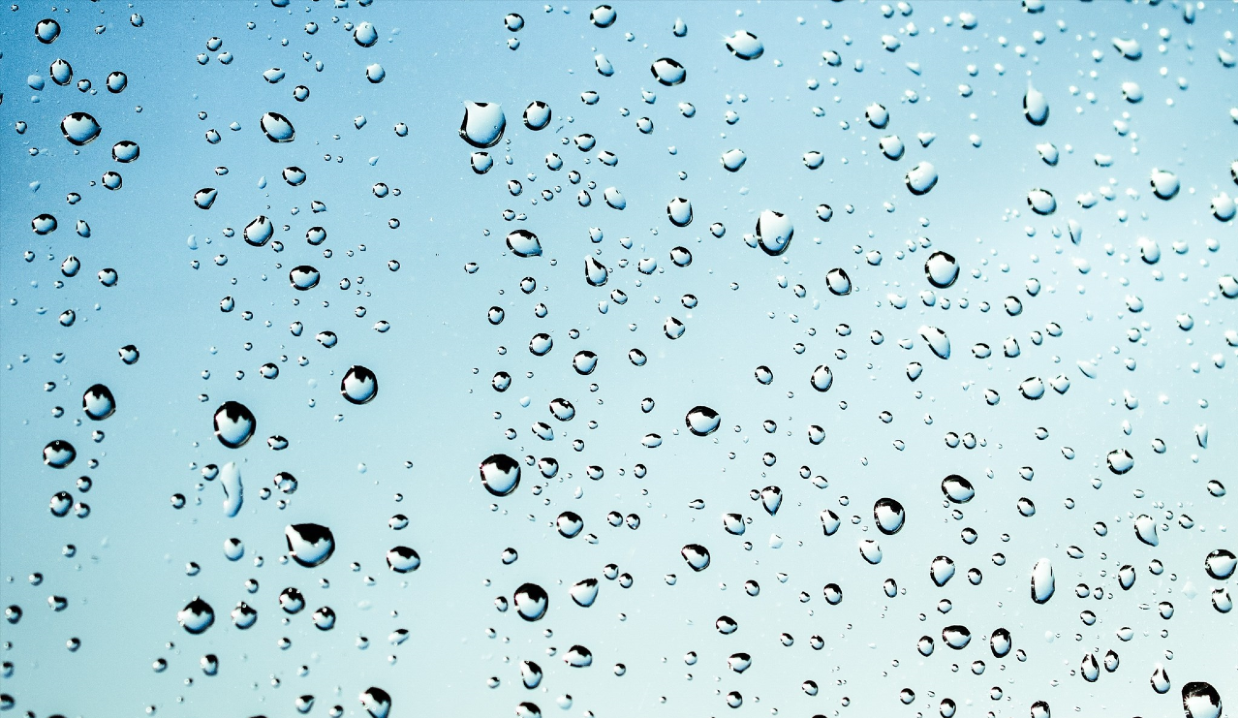
\includegraphics[width=\paperwidth]{Water3.png}};

\node[inner sep=0pt] (background) at (current page.center) {\includegraphics[width=\paperwidth]{WaterBackground1.png}};


\draw (current page.center)node [fill=blue!1!white!10,fill opacity=.3,text opacity=1,inner sep=2cm] { \Huge\centering\bfseries\sffamily\parbox[c][][t]{\paperwidth}{\centering \textcolor{Bittersweet}{WATR 048 - Spring 2022} \\\textcolor{BurntOrange}{Wastewater Treatment}\\[15pt] % Book title
% {\Large A Profound Subtitle}\\[20pt] % Subtitle
{\large Shabbir Basrai}}}; % Author name
\end{tikzpicture}
\begin{center}

\includegraphics[scale=0.5]{SCC_Logo_Primary.png}
\end{center}
\vfill
\endgroup

%----------------------------------------------------------------------------------------
%	COPYRIGHT PAGE
%----------------------------------------------------------------------------------------

\newpage
~\vfill
\thispagestyle{empty}

\noindent Copyright \copyright\ 2022 Shabbir Basrai\\ % Copyright notice
%
%\noindent \textsc{Published by Publisher}\\ % Publisher
%
%\noindent \textsc{book-website.com}\\ % URL
%
%\noindent Licensed under the Creative Commons Attribution-NonCommercial 3.0 Unported License (the ``License''). You may not use this file except in compliance with the License. You may obtain a copy of the License at \url{http://creativecommons.org/licenses/by-nc/3.0}. Unless required by applicable law or agreed to in writing, software distributed under the License is distributed on an \textsc{``as is'' basis, without warranties or conditions of any kind}, either express or implied. See the License for the specific language governing permissions and limitations under the License.\\ % License information, replace this with your own license (if any)

\noindent \textit{Revision Date: April, 2022} % Printing/edition date

%----------------------------------------------------------------------------------------
%	TABLE OF CONTENTS
%----------------------------------------------------------------------------------------

%\usechapterimagefalse % If you don't want to include a chapter image, use this to toggle images off - it can be enabled later with \usechapterimagetrue

\chapterimage{WastewaterTreatmentPlantAerialBandW.jpg} % Table of contents heading image

\pagestyle{empty} % Disable headers and footers for the following pages

\tableofcontents % Print the table of contents itself

\cleardoublepage % Forces the first chapter to start on an odd page so it's on the right side of the book

\pagestyle{fancy} % Enable headers and footers again

%----------------------------------------------------------------------------------------
%	PART
%----------------------------------------------------------------------------------------

\part{Part I}

%----------------------------------------------------------------------------------------
%	CHAPTER 1
%----------------------------------------------------------------------------------------

% \chapterimage{chapter_head_2.pdf} % Chapter heading image

% \chapter{Text Chapter}

% \section{Paragraphs of Text}\index{Paragraphs of Text}

\chapterimage{Dewatering.jpg} % Chapter heading image

\chapter{Theory - Part I}

\section{Background}
\subsection{Definition of Wastewater}

Wastewater is human polluted water from home and industries. This includes water from:
\begin{itemize}
\item Flushing toilets and urinals  - blackwater.
\item Bathing, showering, and washing clothes and dishes  - greywater.
\item Commercial and industrial activities.
\item ...and often included as wastewater is the storm water which contain pollutants washed off inhabited areas - roads, parking lots, and rooftops.
\end{itemize}

\subsection{Why Treat Wastewater}\index{Why Treat Wastewater}
Although nature has an inherent capability to degrade pollutants, given the quantity of wastewater generated from human activities, centralized wastewater treatment plants are required to treat the wastewater and safely return the treated wastewater back to the environment.  Sewers collect the wastewater from homes, businesses, and industries and deliver it to wastewater treatment facilities before it is released back to the environment through its discharge to a water body like a lake, river or ocean, or land, or reused. 

Wastewater treatment is designed to remove:
\begin{itemize}
\item organic matter
\item inorganic  pollutants including plant nutrients - nitrogen and phosphorous\\
\item pathogenic (disease causing) organisms\\
\end{itemize}

\subsection{Benefits of Treating Wastewater}\index{Benefits of Treating Wastewater}
Wastewater treatment protects:
\begin{itemize}
\item The environment
\item Human health
\end{itemize}

Specifically wastewater treatment allows for the following:

\begin{enumerate}
\item \textbf{Mitigates deterioration of the receiving waters' ecosystem }\\
In the receiving waters, inadequately treated wastewater discharge depletes dissolved oxygen levels due to:

\begin{itemize}

\item Nitrogen and phosphorus are essential for plant growth and are common ingredients in fertilizers. However, nutrient-rich wastewater entering a water body such as a lake or river will promote plant and algae growth which will seriously impact its normal aquatic life including fish through a process similar to the following:

\begin{itemize}
\item Nutrient promote algae bloom
\item Algae bloom prevent sunlight to the native plant spieces below the water's surface causing native plants to die
\item The organic material from the dead plants and algae promote growth of aerobic bacteria which will consume the dissolved oxygen in the water resulting in oxygen depletion.
\item The natural aquatic life including fish, frogs, and turtles will not be able to survive under oxygen depleted conditions and will die or leave that zone.
\end{itemize}
\item Other organic material in present in wastewater, will similarly promote growth of aerobic bacteria intensifying the eutrophication of the receiving waters.
\end{itemize}
\item \textbf{Removal of other harmful pollutants}\\
Organic and inorganic pollutants including metals, such as mercury, lead, cadmium, chromium and arsenic can have acute and chronic toxic effects on aquatic species and wildlife including migratory birds, are removed during the wastewater treatment process.
\item \textbf{Removal of pathogens}\\
Wastewater treatment removes parasites and disease-causing pathogens including bacteria and viruses which allow for:
\begin{itemize}
\item People to continue enjoying recreational activities in the receiving bodies of waters such as lakes and rivers
\item Preventing the contamination of fish and other consumable products obtained from the waters
\item Allow the water body to remain as the source of potable water
\end{itemize}
Thus, treating wastewater prevents \hl{eutrophication} which is the process by which a body of water becomes enriched in dissolved nutrients (such as phosphates) that stimulate the growth of aquatic plant life usually resulting in the depletion of dissolved oxygen resulting in a progressive destruction of its normal aquatic lifeforms.
\item \textbf{Reclaim water for recycle or reuse}\\
Besides protecting human health and the environment, wastewater treatment paves way for establishing the reuse or recycle of treated wastewater.  This benefit is particularly important for densely populated areas with limited access to fresh water supplies.  
\end{enumerate}

\newpage
\section{Wastewater Constituents}
	\subsection{Organics}
		\begin{itemize}
			\item The main reason for treating domestic wastewater is to remove the organic matter.  
			\item Organics are substances containing carbon, hydrogen and oxygen, and some of which may be combined with nitrogen, sulfur or phosphorous.
			\item About 50 percent of the solids present in wastewater are organic.  This fraction is generally of animal or vegetable life, dead animal matter, plant tissue or organisms, and also include synthetic organic compounds.
			\item The principal organic compounds present in domestic wastewater are proteins, carbohydrates and fats together with the products of their decomposition.
			\item Organics are subject to decay or decomposition through the activity of bacteria and other living organisms.  \hl{Since the organic fraction can be driven off at high temperatures, they are also called \textbf{volatile solids}}.\
			\item \emph{Organics in wastewater is typically quantified in terms of oxygen required to oxidize the carbon based material present} in wastewater using the following methods:\\
		\end{itemize}
\subsubsection{Biochemical Oxygen Demand (BOD)}\index{Biochemical Oxygen Demand (BOD)}

			  %     \begin{enumerate}[i.]
			  %     	\definecolor{shadecolor}{RGB}{220,220,220}
					% %%%%%%%%%%%
					% % LEVEL 4 %
					% %%%%%%%%%%%
			  %     	\begin{snugshade*}
			  %     		\item \noindent\textsc{Biochemical Oxygen Demand (BOD)}%@@@@@@@@@@@@@@@@@@%
			  %     	\end{snugshade*}					
			      	\begin{itemize}
			      		\item Oxygen is required for the consumption of organic matter by aerobic bacteria
			      		\item BOD test measures the depletion of oxygen in a wastewater sample over a five day period
			      		\item BOD measures the organic content in terms of oxygen required for the microorganisms to consume the organic material present

			      		\item BOD is typically measured as BOD$_5$ which is the oxygen demand of the wastewater measured after 5 days of the initiation of the test.
			      		\item The test involves incubating a known dilution of wastewater in a 300 ml bottle for 5 days at 20\si{\degree}C.  The dissolved oxygen (DO) content at the start and end of the incubation period is used for calculating the BOD.
			      		\item For the test to be considered valid, the following criteria need to be met: 1) DO consumption during the test must be at least 2 mg/l, 2) DO remaining at the end of the test must be at least 1 mg/l, and 3) DO consumed in blank should be 0.2 mg/l or less
			      		      			
			      		\item BOD is a parameter to measure the strength of wastewater and the measurement of the wastewater treatment plant or treatment process influent and effluent BOD is standard practice to measure its performance.  Typical domestic wastewater BOD is about 200-250 mg/l.
			      		\item The oxygen consumed by the microorganisms during the BOD test is primarily for: 1) Oxidizing the carbonaceous material (cBOD – carbonaceous BOD), and 2) Oxidizing nitrogenous constituents such as ammonia (nBOD – nitrogenous BOD).
			      		\item Thus, BOD (Total) = cBOD + nBOD.  The cBOD and nBOD is measured by adding certain chemical inhibitors which will inhibit the bacteria responsible for consuming the nitrogenous matter, thus measuring only the cBOD as part of the BOD test.
			      		\item Since not all of the organics is metabolized in the 5 days of the regular BOD test, certain wastewater discharge permits require reporting of the ultimate BOD value (BOD$_U$)\\
			      	\end{itemize}

			    \subsubsection{Chemical Oxygen Demand (COD)}\index{Chemical Oxygen Demand (COD)}
			      	% \begin{snugshade*}
			      	% 	\item \noindent\textsc{Chemical Oxygen Demand (COD)}%@@@@@@@@@@@@@@@@@@%
			      	% \end{snugshade*}		  
			      	\begin{itemize}
			      		\item The COD test involves using chemical oxidizers to measure the oxygen demand of the wastewater.
			      		\item As the chemical oxidizers will oxidize other constituents present, including inorganic matter, the COD value of wastewater will be higher than the BOD.  
			      		\item The COD test can be conducted rather quickly than the 5 day BOD test, it is an effective method to quantify the wastewater strength and process efficiencies and allow operators to make timely process adjustments.
			      	\end{itemize}


		
			\hl{BOD measures the amount of oxygen required by the microorganisms present to consume the organic material while COD measures the chemical oxidation required to oxidize all chemicals including organics present in wastewater.  BOD value of typical domestic sewage is about 200 - 250 mg/l while the COD value ranges from 300 - 450 mg/l.  Typical BOD:COD ratio ranges from 0.5-0.8.}\\


\subsection{Solids}\index{Solids}
% 		\pagebreak
% 				\begin{snugshade*}
% 			\item \noindent\textsc{Solids}
% 		\end{snugshade*}	
		Like BOD, wastewater solids is another critical parameter for establishing the wastewater strength and determining treatment process efficiencies. 
		\begin{itemize}
			\item The \texthl{solids can be classified as suspended or dissolved} based upon its ability to pass through a standardized filter paper.
			\item When the wastewater is filtered:
			      \begin{itemize}
			      	\item the residual solids remaining on the filter paper after drying in an oven at 103\si{\degree}C is the \hl{suspended solids} portion, and 
			      	\item the solids remaining after drying the filtrate are the \hl{dissolved solids}.
			      \end{itemize}
			\item Suspended solids include larger floating particles and consist of sand, grit, clay, fecal matter, paper, pieces of wood, particles of food and garbage, and similar materials.
			\item Suspended solids can be categorized based upon its settling characteristics as:
			      \begin{itemize}
			      	\item \hl{Settleable}
			      	\item \hl{Non-settleable}
			      	      \begin{itemize}
			      	      	\item \hl{Colloidial}-small, charged (typically negative) particles which do not settle easily.  Some of the colloidial particles are small enough to pass through the filter paper used for filtering the suspended solids
			      	      	\item \hl{Floatable}-example oil and grease and small plastics
			      	      \end{itemize}
			      \end{itemize}
			\item Dissolved solids in wastewater include organics.  However, the major elements of dissolved solids are inorganic ions such as Ca$^{+2}$, Mg$^{+2}$, Cl$^-$, SO$_4$ $^{-2}$ , HCO$_3$ $^-$, Fe$^{+2}$, PO$_4$ $^{-3}$, NO$_3$ $^-$.  These ions are part of the dissolved salts such as sodium chloride (NaCl), calcium bicarbonate (Ca(HCO$_3$)$_2$), magnesium phosphate (Mg$_3$PO$_4$) and others which are normally present in water and wastewater. 
			      \begin{itemize}
			      	\item Conductivity or electrical conductance (EC) measurement is typically conducted as the wastewater enters the plant as \hl{conductivity provides an indirect and simple measure of the amount of dissolved solids present.}  
			      	\item Conductivity or electrical conductance (EC) is a measure the amount of electrical current that can be conducted by a solution.  
			      	\item The conductance of electricity in a solution is due to the presence of dissolved inorganic ions 
			      	\item The higher the concentration of these ions, the higher is the conductivity. 
			      	\item \underline{Conductivity is measured in the units of mhos/cm or Siemens/cm.}  (Note:  mhos is the reverse of ohm which is a measure of resistance).
			      	\item Typical wastewater conductivities range from 50 to 1500 S/cm
			      \end{itemize}
			\item Both suspended and dissolved solids can be either \hl{volatile (organic)} or \hl{fixed (inorganic)}.
			\item \hl{Total Solids is thus a sum of TSS and dissolved solids or volatile and fixed solids.}
			      \begin{itemize}
			      	\item The volatile solids are typically of plant or animal origin .
			      	\item The fixed solids include sand, gravel and silt as well as the dissolved salts.
			      \end{itemize}
			      \begin{minipage}{0.5\textwidth}
			      	\item The volatile or fixed fractions are quantified by incinerating the solids in a muffler furnace at 550\si{\degree} which removes only the volatile solids leaving only the fixed solids behind.
			      	\item In terms of the size of the solids, the distribution is approximately thirty percent suspended and about seventy percent dissolved solids - which includes the colloidal particles which have passed through the filter paper.\\ 
			      	\item As primary treatment process involve settling of solids, establishing the settleable portion of the suspended solids is important.\\  
			      	\item \hl{The settleable solids are quantified using an Imhoff cone and are reported in ml/L}.  Imhoff cone is a 1 liter, clear cone shaped container, with volume graduations (ml) at the bottom.
			      						
			      \end{minipage}	
			      \begin{minipage}{0.5\textwidth}
			      	\begin{center}
			      		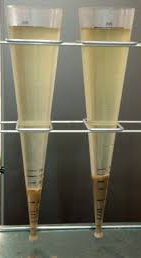
\includegraphics[scale=0.7]{ImhoffCone}\\
			      		Imhoff Cone\\
			      		\textit{Note the ml markings at the bottom of the cone}
			      		
			      		
			      	\end{center}
		      \end{minipage}
%			      \end{minipage}
			      	\item One factor which affects settleability is the conveyance time of the sewage to the treatment plant. 			
			      	\item The settleable component of the suspended solids will decrease as the sewage becomes more septic due to longer conveyance times.
			\item Influent and effluent total suspended solids are measured to establish the overall treatment and individual process efficiencies.  
			\item Volatile solids measurements before and after biological processes such as secondary treatment and digestion provide information on the process efficiency.\\
		\end{itemize}

% 			\end{enumerate}
	\subsubsection{Summary of Wastewater Solids}\index{Summary of Wastewater Solids}		
% 			\begin{snugshade*}
% 				\item \noindent\textsc{Summary of Wastewater Solids}
% 			\end{snugshade*}
			\begin{itemize}
				\item Solids in wastewater can be categorized as dissolved or suspended
				      \begin{itemize}
				      	\item Suspended solids can be further categorized as settleable or unsettleable
				      \end{itemize}
				\item Solids can also be categorized as organic (aka: volatile) or inorganic (aka: fixed)
				\item Colloidial particles are small sized particles some of which pass through the filter and accounted as part of dissolved solids
				\item TSS - Total Suspended Solids are the solids that are captured on the filter paper upon filtration of the wastewater sample.  
				\item Wastewater samples typically analyzed for TSS include:  plant, primary and secondary processes - influent and effluent.  TSS is reported in mg/l
				\item TS - Total Solids are solids content of sludge.  TS of sludge is established by drying a preweighed quantity of sludge in an oven and is typically reported as \% solids - which is how many parts (by weight) of solids per 100 parts (by weight) of sludge.
				\item Volatile solids are solids that are removed when the solids are incinerated at 550C.  The solids that remain after incineration are fixed or non-volatile or inorganic solids.
			\end{itemize}
	\subsubsection{Wastewater Solids Content}\index{Wastewater Solids Content}			
% 			\begin{snugshade*}
% 				\item \noindent\textsc{Typical influent wastewater contains:}
% 			\end{snugshade*}
			\begin{itemize}
				\item Less than 0.1\% total solids.  Total solids concentration in typical wastewater is about 750mg/l
				\item The total solids are 50\% organic (volatile) and 50\% inorganic (fixed)
				\item Of the total solids, dissolved solids constitute about 70\% of the solids and the remaining 30\% solids are suspended solids
				\item 40\% of the dissolved solids are volatile the remaining 60\% are fixed
				\item 70\% of the suspended solids are volatile and the remaining 30\% are fixed
			\end{itemize}
			% \clearpage\thispagestyle{empty}
			\begin{figure}[!htbp]
			\vspace{2cm}
				\begin{center}
					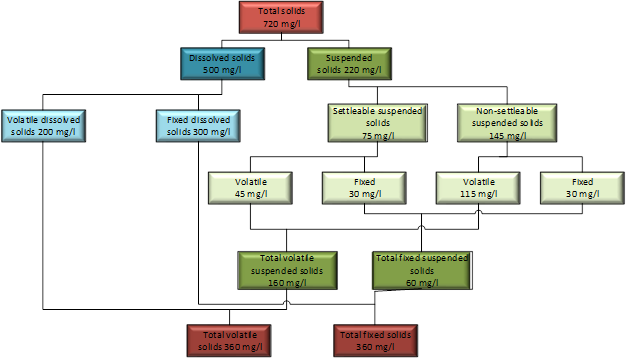
\includegraphics[scale=0.8]{WastewaterSolids}\\
					\caption{Typical Wastewater Solids Concentrations}
				\end{center}
				\end{figure}
% % 			\end{enumerate}
				
\subsection{Nutrients}\index{Nutrients}	
% 			\begin{snugshade*}
% 				\item \noindent\textsc{Nutrients}
% 			\end{snugshade*}	
			\begin{itemize}
				\item Plant nutrients - nitrogen and phosphorous, present in wastewater effluent discharge, promote growth of plant and algal matter in the receiving waters causing destruction of the normal aquatic life mainly due to oxygen depletion - eutrophication.
				      
				\item Because of the potential impacts of the presence of these nutrients in wastewater effluent on the receiving waters,  limits on the levels of these nutrients is typically stipulated in the treatment plant's wastewater discharge permit.
				      
				\item Typically, conventional secondary treatment processes are designed primarily remove the organics from the wastewater.  Secondary treatment process designed to additionally remove nutrients is deemed as tertiary or advanced treatment is termed as Biological Nutrient Removal (BNR).
			\end{itemize}
	\subsubsection{Nitrogen}\index{Nitrogen}				
% 			\begin{enumerate}%@@@@@@@@@@@@@@@@@@%
% 				\definecolor{shadecolor}{RGB}{220,220,220}
% 				\begin{snugshade*}
% 					\item \noindent\textsc{Nitrogen}%@@@@@@@@@@@@@@@@@@%
% 				\end{snugshade*}

	\textbf{Forms of nitrogen:}\\	
% 				\begin{itemize}
% 					\item Forms of nitrogen:\\
					      \begin{itemize}
					      	\item About 60\% of nitrogen in wastewater is present as ammonia nitrogen (about 60\%).  The ammonium nitrogen is present either in the form of ammonia (NH$_3$ ) or as ammonium (NH$_4^+$ ) ion.   These two forms can rapidly change from one to the other depending on pH and temperature.  Under low pH (acidic) or neutral conditions – pH less than or equal to 7, ammonia exists mostly as ammonium.  Ammonia becomes the dominant form as the pH increases to 8 and beyond.
					      	\item The other dominant form of nitrogen, about 40\% of the total nitrogen is as organic nitrogen
					      	\item Nitrogen measured as Total Kjeldahl Nitrogen (TKN) which is the sum of the organic nitrogen and the ammonia nitrogen concentrations.  Total inorganic nitrogen is the total concentration of ammonia nitrogen, NO3-, and NO2-.   Table provides the concentrations and forms of nitrogen in wastewater.
					      \end{itemize}
					      \setlength{\arrayrulewidth}{0.7mm}
					      \setlength{\tabcolsep}{8 pt}
					      \renewcommand{\arraystretch}{0.8}
					      \begin{center}
					      \begin{figure}[!htbp]
					      	\noindent \begin{tabular}[!htbp]{ |p{6cm}|p{2.0cm}|p{2.5cm}|p{2.cm}|}
					      	\hline
					      	\multicolumn{4}{|c|}{\textbf{Forms of Nitrogen in Wastewater}} \\
					      	\hline
					      	%\thead{A Head} & \thead{A Second \\ Head} & \thead{A Third \\ Head} \\
					      	%\hline%
					      	
					      	\hspace{1.8 cm}Forms of Nitrogen & \hspace{0.25 cm} Formula & \hspace{.4 cm} Found in & \hspace{.4 cm} Typical \newline \hspace{.2 cm}Concentration\\
					      	\hline
					      	\small Ammonia/Ammonium & \small NH$_3$/NH$_4^{\enspace +}$ &  \small Influent wastewater & 30-50 mg/l\\
					      	
					      	Total Kjeldahl Nitrogen \newline  \small (Ammonia/Ammonium + Organic Nitrogen) &  \small TKN &  \small Wastewater \newline  \small effluent  & 30-60 mg/l \\
					      	
					      	\small Total Inorganic Nitrogen \newline  \small (Ammonia/Ammonium + Nitrite + Nitrate) & \small TIN &  \small  Wastewater \newline  \small effluent  & 1-40 mg/l \\
					      	
					      	\small Nitrate  & $NO_3^{\enspace -}$ &  \small Nitrified effluent &  \small 1-35 mg/l \\
					      	
					      	\small Nitrate  &  $NO_2^{\enspace -}$ &  \small Partially nitrified effluent &  \small 0.1-2 mg/l \\
					      	
					      	\hline
					      	\end{tabular}
					      	\caption{Forms of Nitrogen}
					      	\end{figure}
					      \end{center}
					      
		\subsubsection{Phosphorous}\index{Phosphorous}			
		\textbf{Forms of phosphorous:}\\
					      \begin{itemize}
					      	\item The principal forms are organically bound phosphorus, polyphosphates, and orthophosphates.
					      	\item Organically bound phosphorus originates from body and food waste and, upon biological decomposition of these solids, is converted to orthophosphates. 
					      	\item Polyphosphates originate from synthetic detergents and are hydrolyzed to orthophosphates. Thus, the principal form of phosphorus in wastewater is assumed to be orthophosphates, although the other forms may exist. Orthophosphates consist of the negative ions PO$_4$$^{3-}$, HPO$_4$$^{2-}$, and H$_2$PO$_4$ $^-$.  These may form chemical combinations with cations (positively charged ions).
					      \end{itemize}

\subsubsection{Oil and Grease}\index{Oil and Grease}	
			Fats, oil and grease in wastewater originate from homes, food establishments and industries.
			\begin{itemize}
				\item Oil and grease content of wastewater is established in the laboratory by extracting it with a solvent - \textit{n}-hexane.  The concentration of oil and grease is reported in mg/l and typical oil and grease content of wastewater ranges from 80 - 120 mg/l
				\item Presence of excessive oils and grease could potentially impact the secondary treatment process
				\item Oils and grease are removed as floatables in primary treatment and sent with the sludge to the digesters
			\end{itemize}
\newpage	
\section{Wastewater Sampling}		
		\begin{itemize}
			\item Field or laboratory measurement of a certain parameter is critical in wastewater treatment operations to obtain information about wastewater characteristics in order to either characterize a wastewater stream, or to monitor a treatment process or for permit compliance.  
			\item A sample is a small part of the whole representing the whole.  Thus, a sample needs to be such that it truly represents the entire population – which in a wastewater operations could be either a wastewater stream, wastewater solids or a chemical used.
		\end{itemize}
		
\subsection{Sampling Methods}\index{Sampling Methods}
\subsubsection{Grab Samples}\index{Grab Samples}
				\begin{itemize}
					\item A grab sample is a sample collected at a specific spot at a site over a short period of time.  
					\item Grab sampling allows for instantaneous analysis of parameters such as pH, dissolved oxygen, chlorine residual, temperature and other parameters which change rapidly with time.
					\item A grab sample represents a snapshot of space and time of a process stream.
					\end{itemize}
\subsubsection{Composite Samples}\index{Composite Samples}
				\begin{itemize}
					\item A composite sample is a collection of discrete samples are combined over a certain period or space and therefore represent the average performance of a wastewater treatment plant or a process during the collection period.\\  
					\item Composite sampling can be either based on:
					      
					      1. constant time interval (time proportioned sampling)\\
					      2. constant wastewater volume interval (flow-proportioned sampling), and\\
					      3. treatment process space - includes samples taken at different depths\\
					      
					\item Composite samples are typically collected using automated samplers which can be programmed to collect samples at pre-established time intervals – for time proportional sampling.
					\item Time and space composite samples are collected by adding equal volumes of samples collected from different times or locations.  
					\item Flow proportional composite samples comprise of volume of each subsample based on flow.\\  
				\end{itemize}
				
			\begin{center}
				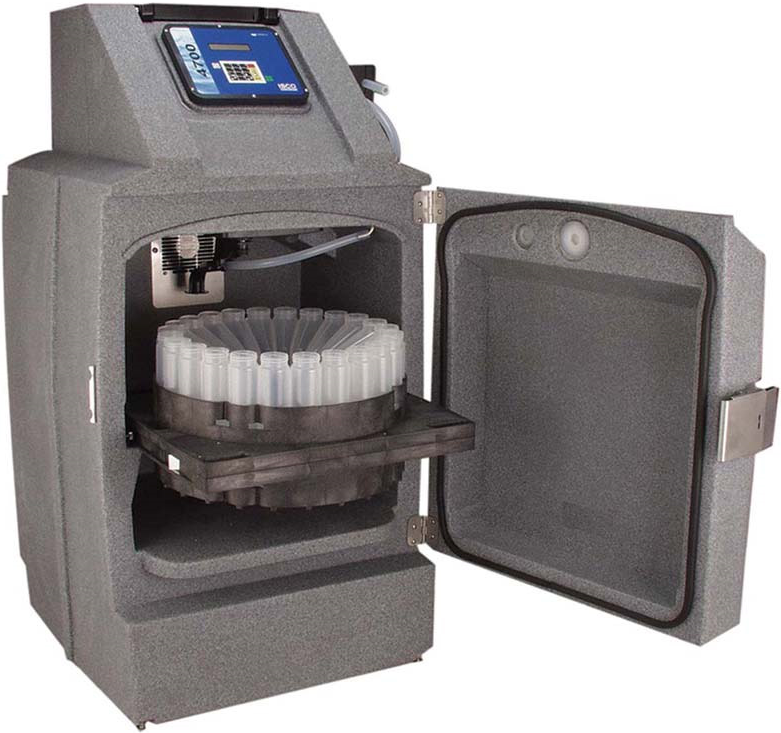
\includegraphics[scale=0.2]{Autosampler} \hspace{2cm} 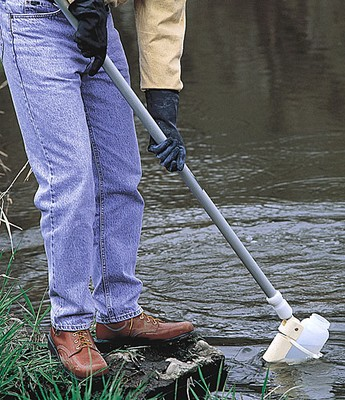
\includegraphics[scale=0.37]{Grabsampler}\\
			\end{center}
			\hspace{2.3cm} Automated Sampler \hspace{2.0cm} \parbox{\textwidth}{Grab Sampling Using a Long Handle Dipper}\\

\subsubsection{Sampling Precautions and Protocols}\index{Sampling Precautions and Protocols}
			\begin{itemize}
				\item Samples should represent the major portion of the process or the process stream and should be taken from places where the mixing is thorough, avoiding dead spots and areas of heavier or lighter loadings. 
				\item The collected sample is invariably exposed to conditions very different from the original source and is subject to change due to chemical and microbiological activity.  
				\item Thus, in order to ensure integrity of sample, sample preservation techniques specific to the analysis to be performed is needed.  
				      \begin{itemize}
				      	\item The preservation technique should not only allow for stabilizing the parameter to be analyzed, it should also not interfere with the analyses.  
				      	\item The common preservation techniques involve use of proper containers, temperature control, addition of chemical preservatives, and observance of the recommended maximum sample holding time.
				      \end{itemize}
			\end{itemize}
			
\subsubsection{Bacteriological Sampling}\index{Bacteriological Sampling}
\begin{itemize}
\item Always collected as a grab
\item A clean, sterile borosilicate glass or plastic bottle containing sodium thiosulfate is used. Sodium thiosulfate is added to remove residual chlorine which will kill coliforms during transit. If the sample is not preserved or maintained under proper conditions until the test is conducted in the laboratory, the test would provide erroneous results
\item Samples must be refrigerated if they cannot be analyzed within 1 hour of collection
\item Samples must be handled with care to prevent contamination and adverse conditions such as prolonged exposure to direct sunlight
\item Maximum holding time for state or federal permit reporting purposes is 6 hours
\end{itemize} 

\subsection{Data Reporting}\index{Data Reporting}	
		\begin{itemize}
			\item Arithmetic mean is typically calculated for reporting data where multiple samples have been collected and analyzed for the same process stream at different times and for reporting average value over a certain time period – daily, monthly etc.\\ \item Arithmetic mean mathematically is calculated by adding all the result values and dividing by the total number of data points.\\
		\end{itemize}
		Mathematically the arithmetic mean is represented as:\\
		$$\bar{x}=\frac{\sum_{i=1}^{n} x^i}{n} = \frac{x_1+x_2+x_3...x_n}{n}$$
		For example:\\
		Arithmetic mean of the following set of data points:  200, 304, 250, 400 is calculated as:\\
		\vspace{10pt}
		Arithmetic Mean = $\frac{200 + 302 + 250 + 400}{4}= 288$\\
		\vspace{10pt}
		For data sets for analysis such as fecal coliform could include values which vary by several orders of magnitudes, using the arithmetic mean to report the average value is not appropriate as the lower or higher values would bias the calculated mean.\\
		\vspace{10pt}
		For example, consider a data set with values:  260, 300, 500, 5,000, 320 and 200.\\
		\vspace{10pt}
		The arithmetic mean = $\frac{260+300+500+5,000+320+200}{6} = 3,444$\\
		Here the 5000 value completely skews the arithmetic mean.
		
		Therefore, for such tests, the geometric mean calculation is used for reporting the average value.\\
		
		
		Mathematically a geometric mean is represented as:\\
		$$\Bigg(\prod_{i=a}^n\Bigg)^{\frac{1}{n}}=\sqrt[n]{a_1*a_2*a_3...a_n}$$
		 
		Calculation method:\\
		1.	Find the product of all the data points (analogous to first calculating the sum of all the data points when calculating the arithmetic mean)\\
		260*300*500*5,000*320*200 = 12,480,000,000,000,000\\
		2.	Raise the product to the inverse of the number of data points\\
		(*Using the power function of a scientific calculator)\\
		Here n (\# data points) = 6 $\implies$ geometric mean = $(12,480,000,000,000,000)^{\frac{1}{6}}   = 482$

\newpage
\section{Collection}\index{Collection}	
The collection system resembles a tree that branches out from the treatment plant to collect the wastewater from individual sources.

\subsection{Wastewater Collection Piping}\index{Wastewater Collection Piping}	
	\begin{itemize}
		\item A \hl{lateral} is the piping that connects the public sewer to the building. 
		\item Laterals flow into larger lines called \hl{mains}.
		\item Mains carry the flow into the largest lines in the system, called \hl{trunk lines}. 
		\item A trunk line is the pipe that brings water into the treatment plant.
	\end{itemize}
\subsection{Sanitary Sewer Systems}\index{Sanitary Sewer Systems}

Sanitary sewer systems collect and convey wastewater from residential, commercial and industrial sources to a centralized wastewater treatment facility for treatment. 

\subsubsection{Storm-water systems}\index{Storm-water systems}

Storm-water systems are designed solely for the conveyance of storm-waters waters directly to streams, rivers, lakes, or the ocean.
 
\subsubsection{Combined sewer systems}\index{Combined sewer systems}
\begin{itemize}
\item Combined sewer systems collect and convey sanitary sewage and urban runoff in a common piping system.
\item Combined sewers could potentially cause serious water pollution problems during combined sewer overflow (CSO) events when wet weather flows exceed the sewage treatment plant capacity.
	\end{itemize}
\begin{center}
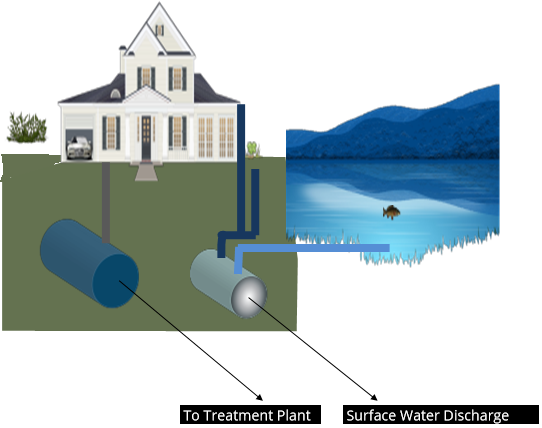
\includegraphics[scale=0.45]{SeperatedSystem1} \hspace{1 cm} 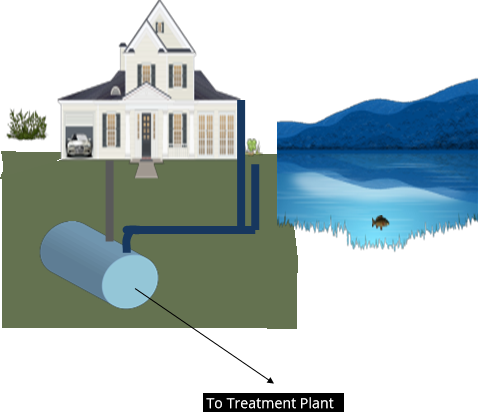
\includegraphics[scale=0.45]{CombinedSystem1}
\end{center}
			\hspace{2.6cm} Separated System \hspace{3.2cm} \parbox{\textwidth}{Combined System}\\

\subsection{Collections Systems Basics}\index{Collections Systems Basics}
	\begin{itemize}
\item The primary type of a collection system is a \hl{gravity system}. A gravity system is so named because the wastewater flows down gradient in the sewer, driven by forces of gravity. 
\item The collection system includes the gravity sewers, force mains, manholes, pumping equipment, and other facilities that collect and convey the water to a wastewater treatment plant. 
\item Sewers are generally laid at a minimum slope to ensure open channel flow through the pipe at a \hl{minimum velocity of 2.0 feet per second}. The minimum velocity is required to ensure that solids do not settle out in the sewer.  
\item When the sewer lines reach a certain depth, the flow must be lifted back through a lift or pump station.  
\item \hl{Lift stations} are built whenever wastewater must be pumped to a higher altitude, whether it's to lift water up so that it can gravity flow or to pump it over a rise or hill.  
\item The discharge from the pump station may be to another gravity sewer at that location or through a pressurized force main. 
\item Key elements of lift stations include a wastewater receiving well (wet-well), pumps and piping with associated valves.
\item The size of the wet well affects the operating of the station. If a wet well is too small, excessive starting and stopping of the pump motors will occur, resulting in premature failure. If the wet well is too large, solids will tend to settle on the bottom, blocking the pump suction line and leading to the generation of hydrogen sulfide and methane.
\item The dry well is the portion of the dry well/wet well pumping station that houses the necessary equipment required to pump the wastewater. The dry well is so named because it is isolated from the incoming wastewater.
\item Centrifugal pumps are the most common type of pump found in wastewater pumping stations. 
\item In the USA, wastewater generated in a typical home is about 70 gal/day/person
\end{itemize}

\newpage
\section{Preliminary Treatment}\index{Preliminary Treatment}

			\begin{itemize}
				\item The objective of preliminary treatment is to remove coarse solids and other large materials often found in raw wastewater
				\item Removal of these materials is necessary to enhance the operation and maintenance of subsequent treatment units\\
				\item Preliminary treatment operations typically include a combination of the following processes:
					\begin{itemize}
						\item Screening
						\item Grinding or shredding
						\item Flow measurement
						\item Grit removal
						\item Pre-aeration
						\item Flow equalization
					\end{itemize}
			\end{itemize}

				
		\subsection{Process Elements of Preliminary Treatment}\index{Process Elements of Preliminary Treatment}	
			
		\subsubsection{Screening}\index{Screening}
					\begin{itemize}
						\item Screening is typically the first unit in a preliminary treatment
						\item Screening allows for the capture of coarse solids as pieces of cloths garbage so as to protect pumps and other units from clogging. 
						\item Screens may consist of vertical or inclined bars (bar racks or bar screens), wire mesh or perforated plates having either circular or rectangular openings. 
						\item Screens remove the large, entrained, suspended or floating solids such as pieces of wood, cloth, paper, plastics, garbage, etc.
						\item Debris collected on the screen can be cleaned manually or automatically using chain driven rakes 
						\item The retained material at screens - screenings, is collected and hauled to landfill for disposal
						\item The quantity of screenings removed varies by location and is a function of the clear opening of the screen.
						\item Barmuinitors combine the function of a screen and a grinder.  The ground material is returned to the wastewater flow for removal during primary treatment.
					\end{itemize}

\begin{figure}
\begin{center}
    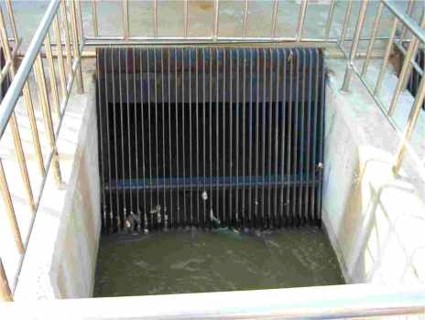
\includegraphics[width=0.7\linewidth]{Barscreen}\\

Barscreen - No rakes
\end{center}
  \end{figure}
  

		\subsubsection{Grinding and Shredding}\index{Grinding and Shredding}

					\begin{itemize}
\begin{minipage}{\textwidth}	\item Comminutor(Grinder) consist of fixed, rotating or oscillating teeth or blades, acting together to reduce the solids to a size which will pass through fixed or rotating screens grind rags into small chunks
\item The comminutors are installed in wastewater channel and they grind the larger solids without actually removing them from the wastewater.  These devices may be installed before the screens or as a combination of screen and cutters (barmunitors).
					\end{minipage}	
					\end{itemize}
					\begin{minipage}{\textwidth}
					\begin{center}
      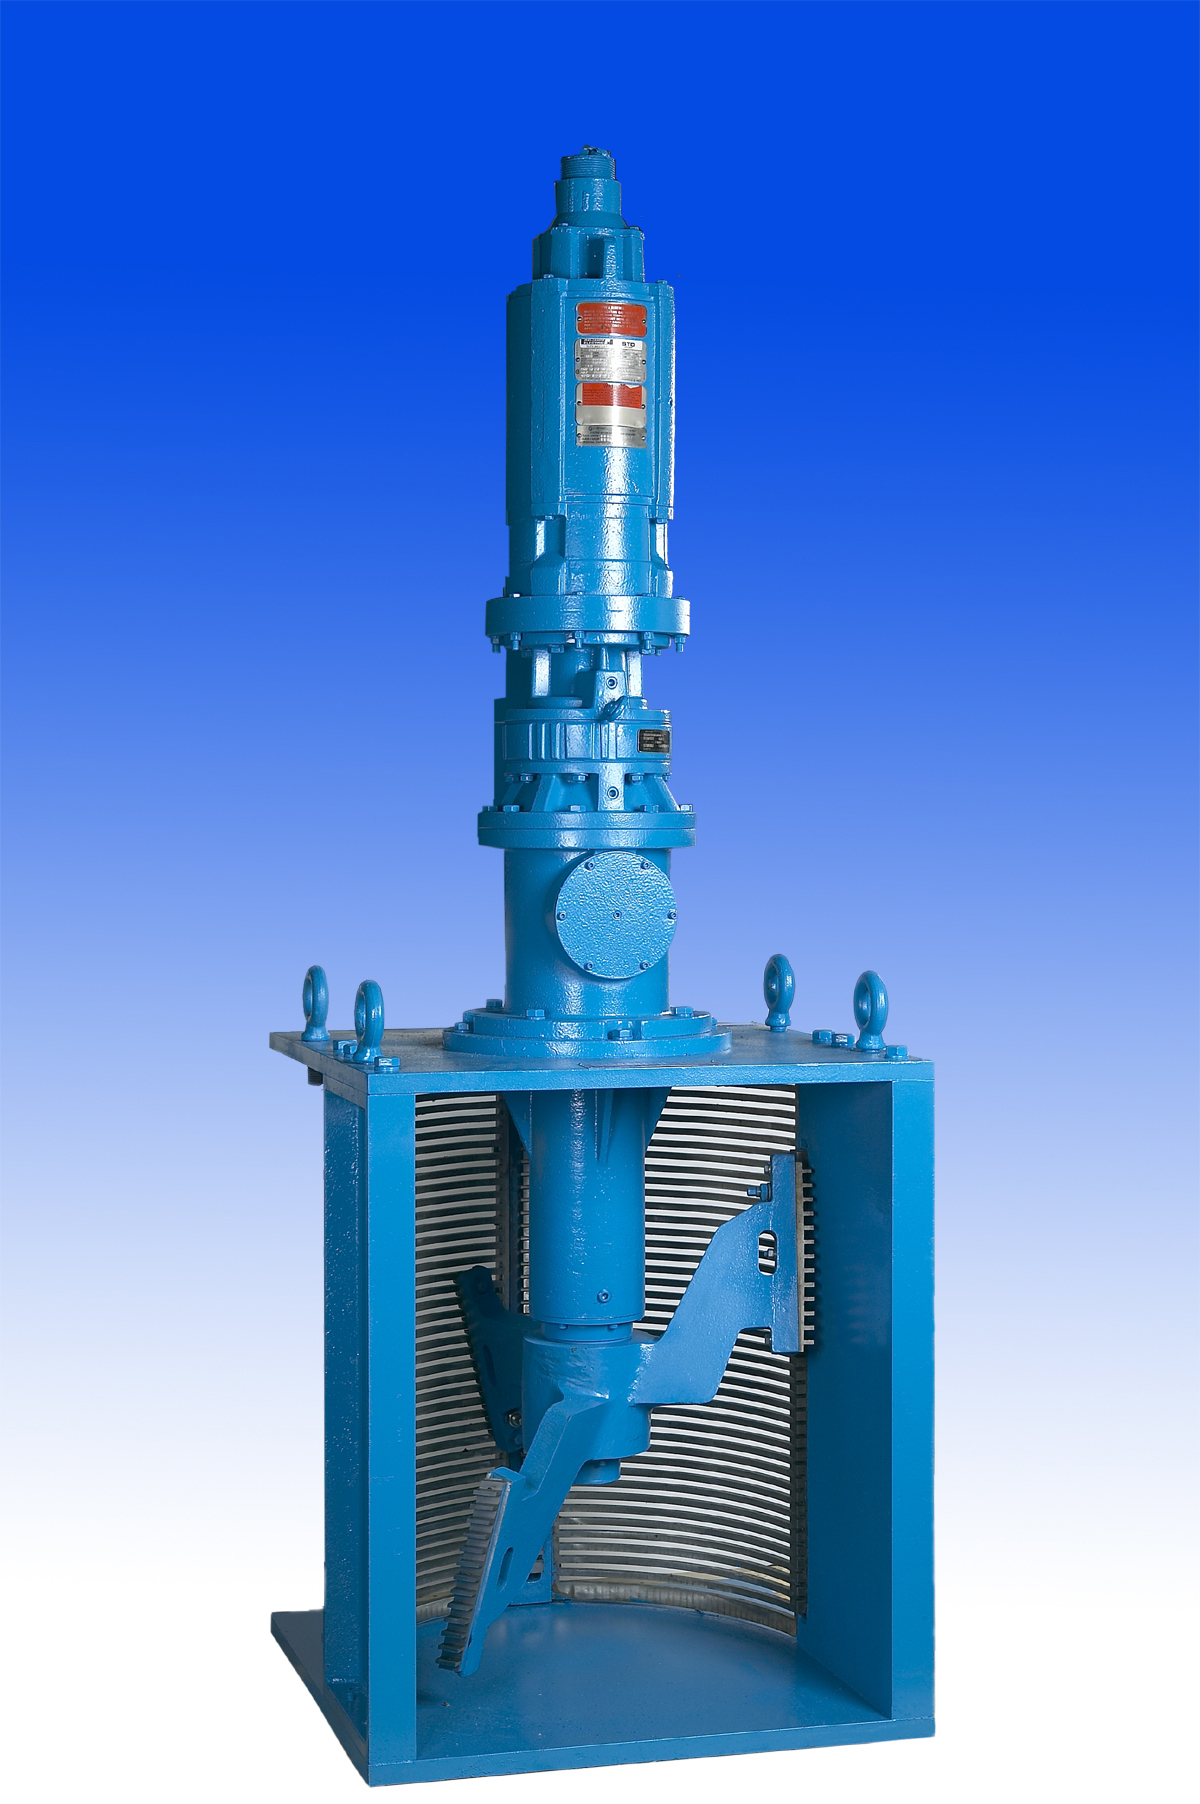
\includegraphics[width=0.3\linewidth, height=70mm]{Comminutor}\\
      Comminutor\\
\end{center}
    \end{minipage}
  
		\subsubsection{Flow Measurement}\index{Flow Measurement}
					\begin{itemize}
						\item Wastewater flow to a treatment plant is not constant but varies in a diurnal (daily) pattern reflecting domestic water use activity.
						\item Continuous flow measurement is necessary in order to monitor diurnal variations in flow which may affect treatment plant efficiency.\\
						\item Devices used for flow measurement as part of the preliminary treatment can be placed in a channel or in a pipe.
					\end{itemize}


		\subsection{Grit Removal}\index{Grit Removal}
						\begin{itemize}
							\item Grit includes sand, gravel, cinder, eggshells, bone chips, seeds, coffee grounds, and large organic particles, such as food waste.
							\item Purpose of Grit removal:
								\begin{itemize} 
									\item to protect mechanical equipment from abrasion and abnormal wear 
									\item to reduce clogging caused by deposition of grit particles in pipes and channels, and 
				\item to prevent loading the treatment plant with inert matter that might interfere with the operation of treatment units such as anaerobic digester and aeration tanks.
			\end{itemize}
		\item Removal of organic material along with the grit is undesirable for two reasons:
			\begin{enumerate}
				\item It causes odor issues, and 
				\item Organic matter is a potential source of energy (digester gas)
			\end{enumerate}
		\item Grit Disposal: Grit removed is typically landfilled.
		\item Grit Volume:  The volume of grit collected measured in ft$^3$/MG.
		\item The rate of grit collection can range from 0.5 ft$^3$/MG to 30 ft$^3$/MG.
		\item Wastewater plants having a combined collection system must deal with much larger volumes of grit.
\end{itemize}

\begin{figure}[h!]
  \centering
  \begin{subfigure}[b]{0.46\linewidth}
    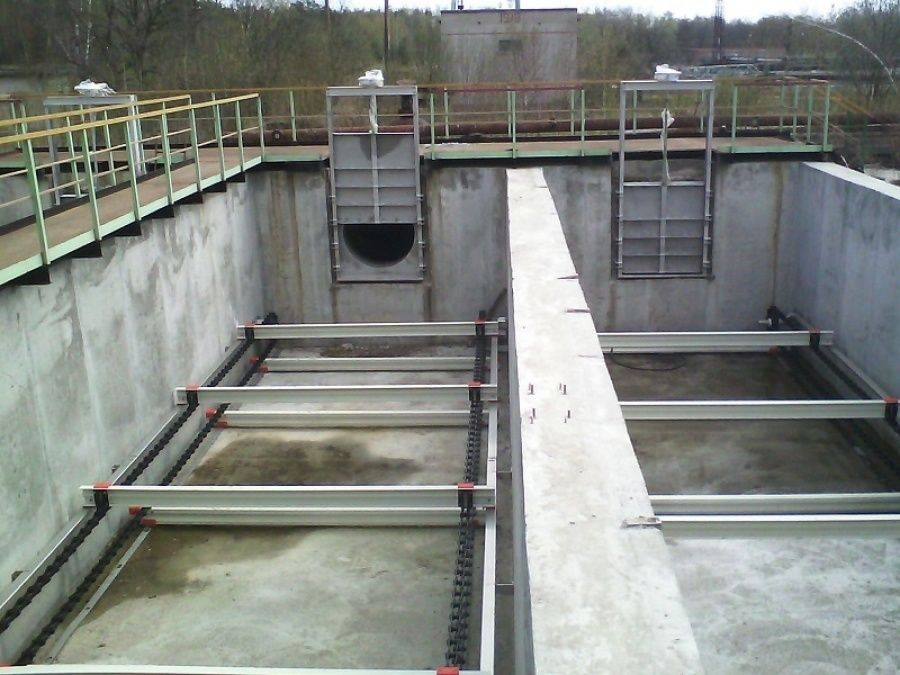
\includegraphics[width=0.8\linewidth]{HorizontalGritChamber}
    \caption{Horizontal grit chamber}
  \end{subfigure}
  \hspace{0.2cm}
  \begin{subfigure}[b]{0.5\linewidth}
    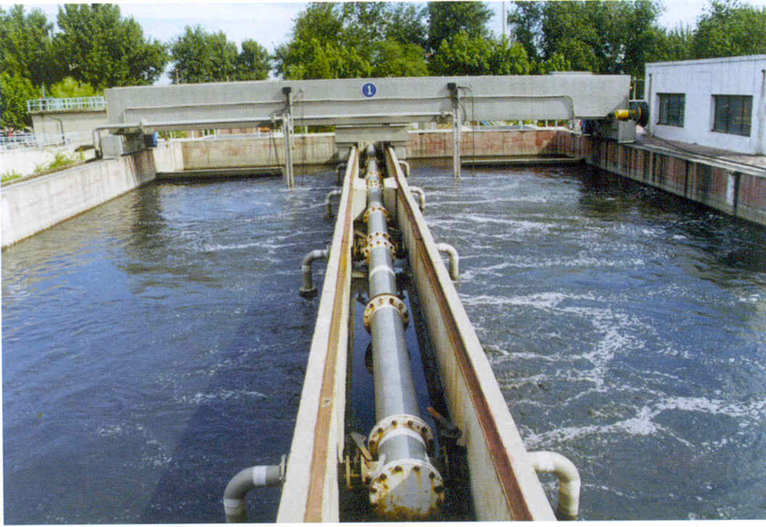
\includegraphics[width=0.8\linewidth]{AeratedGritChamber}
    \caption{Aerated grit chamber}
  \end{subfigure}
\end{figure} 					

\begin{figure}[h!]
  \centering
  \begin{subfigure}[b]{0.47\linewidth}
    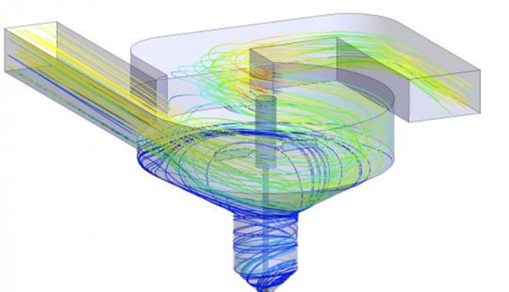
\includegraphics[width=0.8\linewidth]{VortexGritChamber1}
    \caption{Vortex grit chamber design}
  \end{subfigure}
  \hspace{0.2cm}
  \begin{subfigure}[b]{0.43\linewidth}
    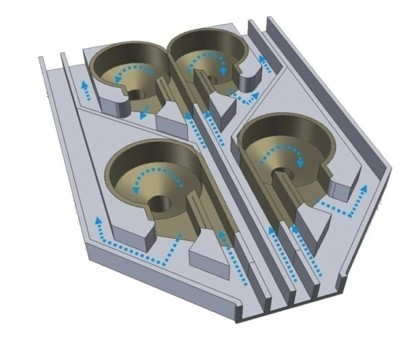
\includegraphics[width=0.8\linewidth]{VortexGritChamber}
    \caption{Vortex grit chamber installed}
  \end{subfigure}
\end{figure} 

\subsection{Pre-aeration}\index{Pre-aeration}	
	\begin{itemize}
		\item Pre-aeration of the wastewater as part of the preliminary treatment may be provided as a separate process or increased detention time in an aerated grit chamber.
		\item Pre-aeration provides the follwoing benefits:
			\begin{itemize}
				\item freshens up wastewater by dissolving oxygen thereby reducing the wastewater septicity
				\item reduction of septicity allows for better settling - solids and BOD removal, in the following primary treatment process
				\item promotes grease separation which facilitates its removal during primary treatment
			\end{itemize}
	\end{itemize}
\subsection{Flow Equalization}\index{Flow Equalization}	

	\begin{itemize}
		\item Flow equalization involves storing a portion of peak flows for release during low-flow periods
		\item It prevents surges and allows for the operation of processes at design flows thus allowing for optimal physical, biological and chemical processes to take place.
		\item It results in saving capital costs as the processes may be built with a treatment capacity which is less than the peak flows
	\end{itemize}
\newpage
\section{Primary Treatment}\index{Primary Treatment}	

\begin{itemize}
\item Synonyms:  primary treatment basin, primary clarifier, sedimentation basin, primaries, clarifier

	
		\item Primary treatment is after preliminary treatment and 				before secondary treatment
		\item Its two main objectives are: 
			\begin{itemize}
				\item Remove settleable solids
				\item Remove floatable solids
			\end{itemize}
		\item This is a physical process which relies on the physical 			properties - how heavy or light the suspended solids particles 		are to effect its separation
		\item Provides quiescent conditions for the influent 					wastewater for the heavier solids to settle and the lighter 			solids to float
		\item Removes settleable solids and floatables
		\item Settled solids are removed as sludge from the bottom of 			the clarifier
		\item Floatable solids including oil and grease are also 				removed, as scum from the surface\\
		\item The shape of the primary clarifier is either rectangular 		or circular
	
		\item Effective solids removal in the primary clarifiers will 			reduce the loading on the expensive secondary treatment 				process.
		\item The amount of solids removed during primary treatment 			may be enhanced by chemical addition - ferric or ferrous 				chloride as a coagulant and anionic polymer as the flocculant.  		This is called Chemically Enhanced Primary Treatment (CEPT).
		\begin{center}
				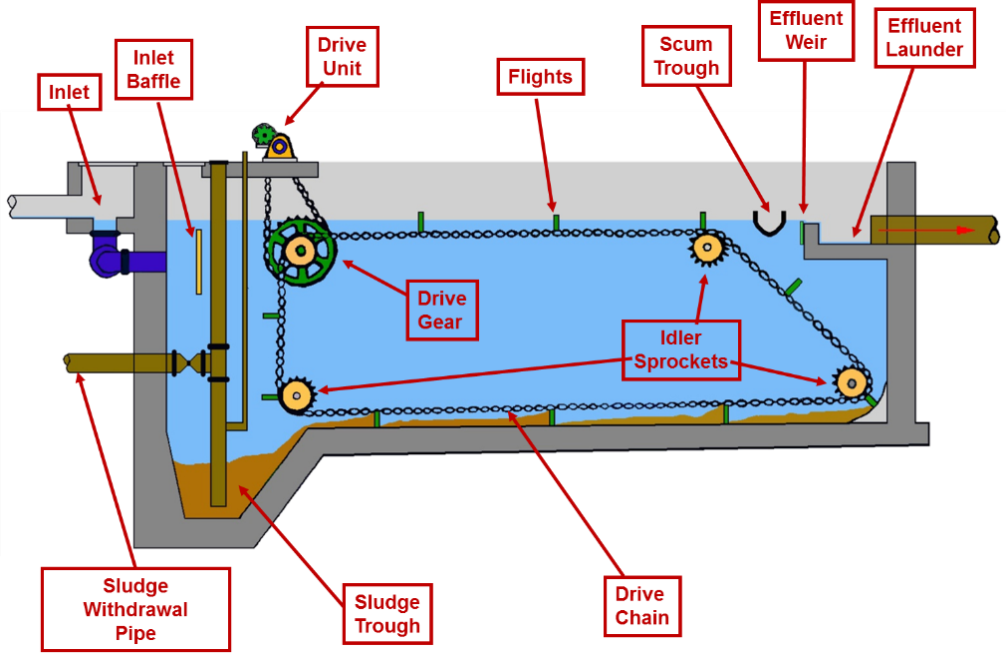
\includegraphics[scale=0.9]{RectangularClarifier}\\
				Cross section of a Rectangular Clarifier\\
				
\includegraphics[scale=0.1]{Blank}\\
				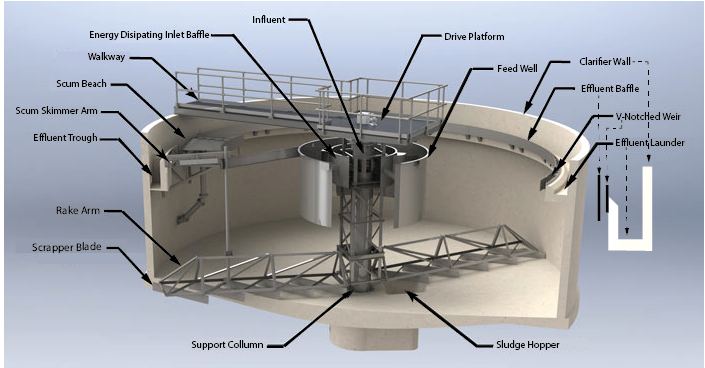
\includegraphics[scale=0.5]{CircularClarifier3}\\
				Cross section of a circular clarifier\\
			\end{center}
				
\includegraphics[scale=0.03]{Blank}\\
\item \textbf{Typical Removal Rates:}\\
\begin{itemize}
\item \hspace{10mm} BOD removal – 25\% to 40\% and about 60\% with CEPT
\item \hspace{10mm} Suspended solids (SS) removal – 40\% to 60\% and about 75\% with CEPT
\item \hspace{10mm} Settleable Solids removal - $>$90\%
\end{itemize}
\end{itemize}


\chapterimage{MathCover.png} % Chapter heading image

\chapter{Math Problems - Part I}

\section{Unit Conversions}\index{Unit Conversions}
\subsection{Example Problems} \index{Example Problems}  
\begin{enumerate}
\item Convert 1000 $ft^3$ to cu. yards:\\
$1000 \cancel{ft^3}*\dfrac{cu.yards}{27\cancel{ft^3}} = 37 cu.yards$\\

\item Convert 3.5 $ft^3/sec$ to MGD:\\
$\dfrac{3.5 \enspace \cancel{ft^3}}{\cancel{sec}} * \dfrac{7.48\cancel {\enspace gal}}{\cancel{ft^3}} * \dfrac{MG}{\enspace 10^6 \cancel{gal}}* \dfrac{1440*60 \enspace \cancel{sec}}{day}=  2.3 \enspace MGD$\\

\item Convert 1,000 L water to lbs:\\
$1000 \enspace \cancel{L}*\dfrac {\cancel{gal}}{3.785 \enspace \cancel{L}}*\dfrac{8.34 \enspace lbs}{\cancel{gal}}\enspace  = 2,203 \enspace lbs$\\
$(Note:8.34 \enspace lbs/gal \enspace is \enspace density \enspace of \enspace water - a \enspace constant)$\\ 
\end{enumerate}


\subsection{Practice Problems} \index{Practice Problems}
\begin{enumerate}
\item Given 1 ft = 30.48 cm and 5,280 ft = mile, convert 3 miles to cm\\


\item The wastewater flow to a treatment plant has a velocity of 61 cm/s. What is this velocity expressed in ft/min. Given: 1 ft = 30.48 cm\\

\item As an operator of a wastewater plant you are treating a flow of 21 MGD, what is the flow in gallons per minute?\\
\end{enumerate}

\newpage

\section{Area \& Volume}\index{Area \& Volume}
 
\subsection{Example Problems} \index{Example Problems} 
\begin{enumerate}
\item The floor of a rectangular building is 20 feet long by 12 feet wide and the inside walls are 10 feet high. Find the total surface area of the inside walls of this building\\
Solution:\\
\begin{center}
\begin{tikzpicture}
	%%% Edit the following coordinate to change the shape of your
	%%% cuboid
      
	%% Vanishing points for perspective handling
	\coordinate (P1) at (-7cm,1.5cm); % left vanishing point (To pick)
	\coordinate (P2) at (8cm,1.5cm); % right vanishing point (To pick)

	%% (A1) and (A2) defines the 2 central points of the cuboid
	\coordinate (A1) at (0em,0cm); % central top point (To pick)
	\coordinate (A2) at (0em,-2cm); % central bottom point (To pick)

	%% (A3) to (A8) are computed given a unique parameter (or 2) .8
	% You can vary .8 from 0 to 1 to change perspective on left side
	\coordinate (A3) at ($(P1)!.8!(A2)$); % To pick for perspective 
	\coordinate (A4) at ($(P1)!.8!(A1)$);

	% You can vary .8 from 0 to 1 to change perspective on right side
	\coordinate (A7) at ($(P2)!.7!(A2)$);
	\coordinate (A8) at ($(P2)!.7!(A1)$);

	%% Automatically compute the last 2 points with intersections
	\coordinate (A5) at
	  (intersection cs: first line={(A8) -- (P1)},
			    second line={(A4) -- (P2)});
	\coordinate (A6) at
	  (intersection cs: first line={(A7) -- (P1)}, 
			    second line={(A3) -- (P2)});

	%%% Depending of what you want to display, you can comment/edit
	%%% the following lines

	%% Possibly draw back faces

	\fill[gray!40] (A2) -- (A3) -- (A6) -- (A7) -- cycle; % face 6
	\node at (barycentric cs:A2=1,A3=1,A6=1,A7=1) {\tiny Floor=W*L};
	
	\fill[gray!50] (A3) -- (A4) -- (A5) -- (A6) -- cycle; % face 3
	\node at (barycentric cs:A3=1,A4=1,A5=1,A6=1) {\tiny Wall - W*H};
	
	\fill[gray!10, opacity=0.2] (A5) -- (A6) -- (A7) -- (A8) -- cycle; % face 4
	\node at (barycentric cs:A5=1,A6=1,A7=1,A8=1) {\tiny Wall - L*H};
	
	\fill[gray!10,opacity=0.5] (A1) -- (A2) -- (A3) -- (A4) -- cycle; % f2
	\node at (barycentric cs:A1=1,A2=1,A3=1,A4=1) {\tiny Wall - L*H};
	
	\fill[gray!40,opacity=0.2] (A1) -- (A4) -- (A5) -- (A8) -- cycle; % f5
	\node at (barycentric cs:A1=1,A4=1,A5=1,A8=1) {\tiny Ceiling=W*L};	
	
	\draw[thick,dashed] (A5) -- (A6);
	\draw[thick,dashed] (A3) -- (A6);
	\draw[thick,dashed] (A7) -- (A6);

	%% Possibly draw front faces

	%\fill[orange] (A1) -- (A8) -- (A7) -- (A2) -- cycle; % face 1
	\node at (barycentric cs:A1=1,A8=1,A7=1,A2=1) {\tiny Wall - W*H};
	


	%% Possibly draw front lines
	\draw[thick] (A1) -- (A2);

	\draw[<->] (-1.8,0.38) -- (-1.8,-1.3)node [midway, above=-1.8mm] {\hspace{-1.3cm}\tiny Height=10'};
	\draw[<->] (-1.6,-1.4) -- (-.3,-2.1)node [midway, above=-2.6mm] {\hspace{-1.3cm}\tiny Length=20'};
	\draw[<->] (2.6,-1.13) -- (0.2,-2.2)node [midway, below=.6mm] {\hspace{1.2cm}\tiny Width=12'};
	\draw[thick] (A3) -- (A4);
	\draw[thick] (A7) -- (A8);
	\draw[thick] (A1) -- (A4);
	\draw[thick] (A1) -- (A8);
	\draw[thick] (A2) -- (A3);
	\draw[thick] (A2) -- (A7);
	\draw[thick] (A4) -- (A5);
	\draw[thick] (A8) -- (A5);
	
	% Possibly draw points
	% (it can help you understand the cuboid structure)
%	\foreach \i in {1,2,...,8}
%	{
%	  \draw[fill=black] (A\i) circle (0.15em)
%	    node[above right] {\tiny \i};
%	}
	% \draw[fill=black] (P1) circle (0.1em) node[below] {\tiny p1};
	% \draw[fill=black] (P2) circle (0.1em) node[below] {\tiny p2};
\end{tikzpicture}\\
\end{center}
2 Walls W*H + 2 Walls L*H= $2*12*10ft^2 + 2*20*10ft^2$\\
$=240+400=\boxed{640ft^2}$\\

2 Walls W*H + 2 Walls L*H + Floor + Ceiling= $2*12*10ft^2 + 2*20*10ft^2 + 2*12*20ft^2$\\
$=240+400+480=\boxed{1,120ft^2}$\\

\item What is the surface area of a cylinder 50 ft diameter and 25 ft height?\\
Solution:\\
\begin{center}
\begin{tikzpicture}[mydashed/.style={dashed,dash phase=2pt}]
\draw (0,0) ellipse (2cm and 0.3cm) node [midway, above=-2.4mm] {\hspace{0.1cm}\tiny{Top Area$=\dfrac{\pi}{4}*D^2$}};
\draw (0,-2.3) ellipse (2cm and 0.3cm) node [midway, below=2.05cm] {\hspace{0.1cm}\tiny{Bottom Area$=\dfrac{\pi}{4}*D^2$}};
\draw [-] (2,-2.3) -- (2,0);
%\draw [<->] (-2,0) -- (2,0); 
\draw [<->] (2.5,-2.3) -- (2.5,0) node [midway, below] {\hspace{2.9cm}Height (h) =25'};
\draw [<->] (-2,-0.4) -- (2,-0.4) node [midway, below=0.7mm] {\hspace{0.1cm}\small{Diameter (D)=50'}};
%\draw [-] (0,-4) -- (2,-2.3);
%\draw [-] (0,-4) -- (-2,-2.3);
%\draw [-] (0,-4) -- (2,-2.3);
\draw [-] (-2,0) -- (-2,-2.3) node [midway, below] {\hspace{4cm}\tiny{Cylinder Surface Area$=\pi*D*h$}};
\draw [-latex, mydashed, line width=1mm, rotate=-90] (0.6,-1.9) arc [start angle=-120, end angle=120, x radius=0.8cm, y radius=2.2cm];
%\draw [-latex, thick, rotate=-95] (0,0) arc [start angle=-190, end angle=160, x radius=1cm, y radius=2cm];
\end{tikzpicture}\\
\end{center}
$Surface \enspace area \enspace of \enspace cylinder=surface \enspace area \enspace of \enspace the \enspace top \enspace  and \enspace bottom \enspace faces + surface \enspace area \enspace of \enspace the \enspace cylinder$\\
$\implies(2*\dfrac{\pi}{4}*D^2)+(\pi*D*h)=2*0.785*50^2+3.14*50*25=\boxed{7,850ft^2}$
\end{enumerate}

\subsection{Practice Problems} \index{Practice Problems}
\begin{enumerate}

\item A cylindrical tank is 10 feet in diameter and 20 feet in height. 'What is the approximate capacity in liters?\\


\item What is the volume of water in a sedimentation basin 80 feet long, 28 feet wide and a 9.5 feet water depth? Give your answer in gallons.\\

\item How many gallons will 1,200 feet of 6-inch pipe hold?\\
\item What is the surface area of a cylinder 80 ft diameter and 25 ft height?  Cylindrical part surface area only. Disregard the floor and roof areas.\\
\item How many gallons of paint will be required to paint the inside walls of a 40 ft long x 65 ft wide x 20 ft high tank if the paint coverage is 150 sq. ft per gallon.  Note:  We are painting walls only.  Disregard the floor and roof areas.\\
\item What is the circumference of a 100 ft diameter circular clarifier?\\
\item If the surface area of a clarifier is 5,025$ft^2$, what is its diameter?\\
\end{enumerate}

\section{Concentration}\index{Concentration}
\subsection{Example Problems} \index{Example Problems}
\begin{enumerate}
\item What is the salt content in mg/l of a 2.5\% salt solution?\\
Solution:
25,000mg/l
\item What is the \% concentration of a solids content in a sludge with 5000 mg/l solids concentration?\\
Solution:\\
0.5\%\\
\end{enumerate}
\subsection{Practice Problems} \index{Practice Problems}

\begin{enumerate}
\item A 6.35\% solution is is equivalent to {\underline{\hspace{1cm}}} mg/l\\
\end{enumerate}

\newpage
\section{Pounds Formula}\index{Pounds Formula}
\subsection{Example Problems} \index{Example Problems}
\begin{enumerate}
\item If the influent wastewater flow is 5 MGD and the BOD concentration is 240 mg/l what is the daily BOD loading in lbs/day?\\
Solution:\\
$\dfrac{lbs \enspace BOD}{day}=5MGD*240mg/l*8.34=\boxed{\dfrac{10,000lbs}{day}}$\\

\item Calculate the lbs of solids in the primary sludge if the sludge flow is 7500 gallons and the solids concentration is 4.5\%.\\
Solution\\
Applying lbs formula:\\
$lbs \enspace solids = \dfrac{7500 \enspace MG}{1,000,000} * 4.5*10,000 *8.34 = \boxed{2,815 \enspace lbs \enspace solids}$\\
\textbf{Note:}\\  
1) 7500 gallons was converted to MG by dividing by 1,000,000\\
$7500 \enspace gallons * \dfrac{1 MG}{1,000,000 \enspace gallons}$\\
2) 4.5\% was converted to mg/l by multiplying by 10,000 as 1\%=10,000mg/l

\end{enumerate}

\subsection{Practice Problems} \index{Example Problems}

\begin{enumerate}
\item An operator dissolves 1,200 lbs of a chemical in 12,000 gallons of water, what is the resultant concentration in mg/l, of the chemical solution?\\
\end{enumerate}

\newpage
\section{Removal Efficiency}\index{Removal Efficiency}

\subsection{Example Problems} \index{Example Problems}

\begin{enumerate}

\item The influent to a trickling filter plant is 200 mg/L and the effluent BOD is 20 mg/L. What is the BOD removal efficiency (\%)?\\
Solution:\\
\vspace{0.3cm}
\tikzstyle{block} = [rectangle, draw, fill=red!40, 
    text width=6em, text centered, rounded corners, minimum height=3em]
\tikzstyle{arrow} = [draw, -latex']
\begin{figure}[!h]
\centering
\begin{tikzpicture}[node distance =1.5cm, auto]
    \draw ++(0,0) node [block] (Process) {Process};
   \node[node distance=1.5in] (dummy_in) [left of=Process] {};
   \node[node distance=1.5in] (dummy_out) [right of=Process] {};
	\node (Removal) [below of=Process, yshift=-0in] {$Removal \enspace Efficiency=?\%$};
    \path [arrow] (dummy_in)-- (Process)  node [above] {\hspace{-4.39cm}$200mg/l$} node [below] {};
    \path [arrow] (Process) -- (dummy_out)  node [above] {\hspace{-1.8cm}$20mg/l$} node [below] {};
   \draw[arrow] (Process) -- (Removal);
\end{tikzpicture}
\end{figure}
\vspace{0.5cm}
$Removal \enspace Efficiency \enspace (\%) = \dfrac{In-Out}{In}*100 \implies \dfrac{200-20}{200}*100=\boxed{90\%}$




\item Calculate the primary clarifier influent solids concentration if its outlet concentration is 60 mg/l and the known clarifier removal efficiency is 75\%?\\
$\dfrac{Actual \enspace  inlet \enspace (X)}{Actual \enspace outlet}=\dfrac{100}{100-Removal \enspace efficiency}$\\ 
$\dfrac{Actual \enspace  inlet \enspace (X)}{60}=\dfrac{100}{100-75}=4$\\
$\implies Actual \enspace inlet \enspace (X)=4*60 = \boxed{240 mg/l}$\\

\item If a primary clarifier consistently operates at 30\% efficiency and produces an effluent which averages 140 mg/l BOD, what is the influent BOD? \\
Solution:\\
\vspace{0.3cm}
\tikzstyle{block} = [rectangle, draw, fill=red!40, 
    text width=6em, text centered, rounded corners, minimum height=3em]
\tikzstyle{arrow} = [draw, -latex']
\begin{figure}[!h]
\centering
\begin{tikzpicture}[node distance =1.5cm, auto]
    \draw ++(0,0) node [block] (Process) {Process};
   \node[node distance=1.5in] (dummy_in) [left of=Process] {In};
   \node[node distance=1.5in] (dummy_out) [right of=Process] {Out};
	\node (Removal) [below of=Process, yshift=-0in] {$Removal \enspace Efficiency=30\%$};
    \path [arrow] (dummy_in)-- (Process)  node [above] {\hspace{-4.39cm}$Xmg/l$} node [below] {\hspace{-4.39cm}$100mg/l$};
    \path [arrow] (Process) -- (dummy_out)  node [above] {\hspace{-3.cm}$140mg/l$} node [below] {\hspace{-3cm}70mg/l};
   \draw[arrow] (Process) -- (Removal);
\end{tikzpicture}
%\caption[MFCC]{Diagrama en bloques del cálculo de las MFCC para un frame.}
%\label{MFCC}
\end{figure}
$\dfrac{Actual \enspace  inlet \enspace (X)}{Actual \enspace outlet}=\dfrac{100}{100-Removal \enspace efficiency}$\\ 
$\dfrac{Actual \enspace  inlet \enspace (X)}{140}=\dfrac{100}{100-30}=1.43$\\
$\implies Actual \enspace inlet \enspace (X)=1.43*140 = \boxed{200 mg/l}$\\



\end{enumerate}

\subsection{Practice Problems} \index{Practice Problems}

\begin{enumerate}

\item What is the \% removal efficiency if the influent concentration is 10 mg/L and the effluent concentration is 2.5 mg/L?\\
\item If a plant removes 35\% of the influent BOD in the primary treatment and 85\% of the remaining BOD in the secondary system, what is the BOD of the raw wastewater if the BOD of the final effluent is 20mg/l \\
\item Calculate the inlet concentration if the outlet concentration is 80 mg/l and the process removal efficiency is 60\%\\
\item Calculate the outlet concentration if the inlet concentration is 80 mg/l and the process removal efficiency is 60\%\\
\end{enumerate}

\newpage
\section{Flow and Velocity}\index{Flow and Velocity}
\subsection{Example Problems}
\begin{enumerate}
\item Calculate the velocity of a 14 MGD flow in a 6 ft wide channel with a water depth of two feet.\\
\begin{center}
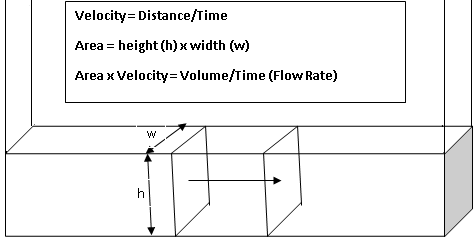
\includegraphics[scale=0.5]{ChannelFlow3}
\end{center}
$Flow (Q) = Velocity (V) * Area (A)$\\
$\implies Flow\Big[ 14 \dfrac{MG}{day}* \dfrac{10^6 gal}{MG} * \dfrac{ft^3}{7.48 gal}*\dfrac{day}{24*60*60sec}\Big]\dfrac{ft^3}{sec} = Velocity(V) \dfrac{ft}{sec}* Area (6 * 2) ft ^2$\\
\vspace{0.2cm}
$\implies 21.7 \dfrac{ft^3}{sec}= V\dfrac{ft}{sec}*12ft^2$\\
$\implies V \dfrac{ft}{sec}= \dfrac{21.7\dfrac{\cancelto{ft}{ft^3}}{sec}}{12\cancelto{}{ft^2}}= \boxed{1.8\dfrac{ft}{sec}}$\\

\item If a chemical is added in a sewer where wastewater is flowing at a velocity of 3.1 feet per second, how many minutes would it take for the chemical to reach the plant 7 miles away?\\
Solution:\\
Min $= \dfrac{1}{3.1}\dfrac{sec}{ft}*\dfrac{5280ft}{mile}*7 miles*\dfrac{min}{60 sec} = \boxed{199 min}$
\\

\item A plastic float takes 9.8 seconds to travel a distance of 25 feet in a wastewater channel. The channel is 3 ft 8 in. wide and the water level in this channel is 28 inches. What is the wastewater flow in GPM\\
Solution:\\
\vspace{0.3cm}
$Q=V*A$\\
$\implies Q=\dfrac{25ft}{9.8s}*\Big((3+\dfrac{8}{12})*\dfrac{28}{12}\Big)ft^2*7.48\dfrac{gal}{ft^3}*60\dfrac{s}{min}=\boxed{9,795\dfrac{gal}{min}}$



\item Calculate the flow, in gpd, that would pass through a grit chamber 2 feet wide, at a depth of 6 inches, with a velocity of 1 ft /sec\\
Solution:\\
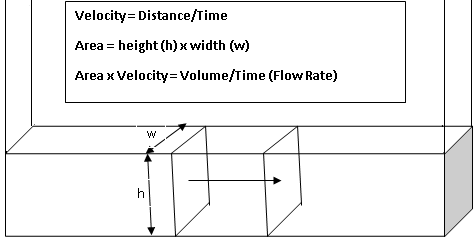
\includegraphics[scale=0.5]{ChannelFlow3}\\
$Q=V*A$\\
$Q=1\dfrac{ft}{s}*(2*0.5)ft^2=1\dfrac{ft^3}{s}$\\
$Q=1\dfrac{\cancel{ft^3}}{\cancel{s}}*\dfrac{(1440*60)\cancel{s}}{day}*7.48\dfrac{gal}{\cancel{ft^3}}=\boxed{646,272\dfrac{gal}{day}}$
\end{enumerate}



\subsection{Practice Problems} \index{Practice Problems}

\begin{enumerate}
\item A wastewater channel is 3.25 feet wide and is conveying a wastewater flow of 3.5 MGD. The wastewater flow is 8 inches deep. Calculate the velocity of this flow.\\

\item A plastic float is dropped into a wastewater channel and is found to travel 10 feet in 4.2 seconds. The channel is 2.4 feet wide and is flowing 1.8 feet deep. Calculate the flow rate of this wastewater in cubic feet per second.\\

\item A 12 inch pipe conveys sewage at 2.6 feet per second.  What is the flow expressed in MGD?

\item A sewer line to a wastewater treatment plant is 12 miles long. If the wastewater is flowing at 2.2 fps, approximately.  How long will it take for wastewater to reach the plant?\\
 
\end{enumerate}
\newpage

\section{Preliminary Treatment}\index{Preliminary Treatment}

\subsection{Example Problems} \index{Example Problems}

\begin{enumerate}

\item At a wastewater treatment plant which receives a flow rate of 650,000 gallons per day, a total of 50 cubic feet of grit was removed for the month. Calculate the rate of grit removal assuming 30 days in a month.\\
Solution:\\
$Grit Removal\dfrac{ft^3}{MG}=50\dfrac{ft^3}{ \cancel{month}}*\dfrac{\cancel{month}}{30\cancel{days}}*\dfrac{\cancel{day}}{650,000\cancel{gal}}*1,000,000\dfrac{\cancel{gal}}{MG}=\boxed{2.6\dfrac{ft^3}{MG}}$

\end{enumerate}

\subsection{Practice Problems} \index{Practice Problems}

\begin{enumerate}
\item On an average a 12.5 yd. load of grit is hauled to the landfill once every 20 days. Plant flow averages 12.5 MGD. Calculate the rate of grit collection in ft$^3$/MG.\\

\item On an average, 2 inches of grit is collected and removed every day in a 2.2 feet wide, 205 feet long grit channel.  Knowing the average flow through that grit channel is 10 MGD calculate the rate of grit collection in ft$^3$/MG\\

\end{enumerate}

\newpage
\section{Primary Treatment} \index{Primary Treatment}
\subsection{Example Problems} \index{Example Problems}
\begin{enumerate}
\item If a clarifier has a capacity of 0.25 MG, what is the detention time in hours if it receives a flow of 3 MGD\\
Solution:\\
$Clarifier \enspace detention \enspace time \enspace (hr) = 	\dfrac{ Clarifier \enspace volume (MG)}{Influent \enspace flow \enspace (MG/hr)}$\\
\vspace{0.5cm}
$Clarifier \enspace detention \enspace time \enspace (hr) = 	\dfrac{0.25\cancel{MG}}{\dfrac{3\cancel{MG}}{\cancel{day}}*\dfrac{\cancel{day}}{24hrs}}=\boxed{2hrs}$\\

\item If a 90 ft diameter primary clarifier operating at water depth of 20 ft is treating a 12MGD flow, calculate the surface loading rate (gal/(day-sq.ft).\\
Solution:\\
$Clarifier \enspace hydraulic \enspace loading \enspace 	\Big(\dfrac{gpd}{ft^2}\Big) =\dfrac{\dfrac{12\cancel{MG}}{{day}}*\dfrac{10^6gal}{\cancel{MG}}}{0.785*90^2 ft^2}=\boxed{1,887gpd/ft^2}$\\


\vspace{0.5cm}
\item What is the weir overflow rate (gpd/ft) when treating a 15 MGD flow in a 105 ft diameter primary sedimentation tank operating at water depth of 20 ft.\\
\vspace{0.5cm}
Solution:\\
\vspace{0.5cm}
$Clarifier \enspace detention \enspace time \enspace (hr) = 	\dfrac{(0.785*105^2*20)\cancel{ft^3}}{\dfrac{15\cancel{MG}}{\cancel{day}}*\dfrac{10^6\cancel{gal}}{\cancel{MG}}*\dfrac{\cancel{ft^3}}{7.48\cancel{gal}}*\dfrac{\cancel{day}}{24hrs}}=\boxed{2.1hrs}$\\
\end{enumerate}

\subsection{Practice Problems} \index{Practice Problems}

\begin{enumerate}


\item A circular clarifier receives a flow of 11 MGD.  If the clarifier is 90 ft. in diameter and is 12 ft. deep, what is: a) the hydraulic/surface loading rate, b) weir overflow rate, and c) clarifier detention time in hours?\\

\item At a 2.5 MGD wastewater treatment plant the primary clarifier has a detention time of 2 hours. How many gallons does this clarifier hold?\\

\end{enumerate}

\newpage

\section{Pumping}\index{Pumping}

\subsection{Example Problems} \index{Example Problems}


\begin{enumerate}

\item How many lbs/day of solids are removed in a clarifier treating a 6 MGD flow if the average inlet concentration is 320 mg/l and its average outlet concentration is 80 mg/l\\
\vspace{0.5cm}
Solution:\\
\vspace{0.5cm}
Applying pounds formula:\\
$\dfrac{lbs \enspace solids \enspace removed}{day}=6MGD*(320-80)\dfrac{mg}{l}*8.34=\boxed{120,096\dfrac{lbs \enspace solids}{day}}$

\item A clarifier has a TSS removal efficiency of 50\%.  If the influent TSS concentration is 220 mg/L, how many lbs/day of TSS are removed if the flow is 10 MGD.  Also, how many cu. ft of sludge is pumped if the sludge has a TS concentration of 5\%.\\
$lbs \enspace solids \enspace removed=(220*0.50)mg/l*10MGD*8.34=9,174lbs \enspace solids \enspace per \enspace day$
$$\dfrac{ft^3\enspace sludge}{day}= \dfrac{9,174 \enspace \cancel{lbs \enspace solids}}{day} * \dfrac{1 \enspace \cancel{lb \enspace sludge}}{0.05\enspace \cancel{lbs \enspace solids}}*\dfrac{\cancel{gal \enspace sludge}}{8.34\cancel{lb \enspace sludge}}*\dfrac{ft^3 \enspace sludge}{7.48 \enspace \cancel{gal}}=\boxed{2,941\dfrac{ft^3 \enspace sludge}{day}} $$

\item Given the tank is 10ft wide, 12 ft long and 18 ft deep tank including 2 ft of freeboard when filled to capacity. How much time (minutes) will be required to pump down this tank to a depth of 2 ft when the tank is at maximum capacity using a 600 GPM pump\\
Solution:\\
\vspace{0.5cm}

\begin{tikzpicture}

\pgfmathsetmacro{\cubexx}{4}
\pgfmathsetmacro{\cubeyy}{1.5}
\pgfmathsetmacro{\cubezz}{2}
\pgfmathsetmacro{\cubex}{4}
\pgfmathsetmacro{\cubey}{0.5}
\pgfmathsetmacro{\cubez}{2}
\pgfmathsetmacro{\cubexxx}{4}
\pgfmathsetmacro{\cubeyyy}{4}
\filldraw [fill=cyan!10!white, draw=black] (0,-\cubey,0) -- ++(-\cubexx,0,0) -- ++(0,-\cubeyy,0) -- ++(\cubexx,0,0) -- cycle ;
\filldraw [fill=cyan!0!white, draw=black] (0,-\cubey,0) -- ++(0,0,-\cubezz) -- ++(0,-\cubeyy,0) -- ++(0,0,\cubezz) -- cycle;
\filldraw [fill=cyan!10!white, draw=black] (0,-\cubey,0) -- ++(0,0,-\cubezz) -- ++(0,-\cubeyy,0) -- ++(0,0,\cubezz) -- cycle;
%\filldraw [fill=cyan!10!white, draw=black] (0,-\cubey,0) -- ++(-\cubexx,0,0) -- ++(0,0,-\cubezz) -- ++(\cubexx,0,0) -- cycle;
%%%\draw (0,-0.5,0) -- ++(-\cubex,0,0) -- ++(0,-\cubey,-\cubez) -- ++(\cubex,0,0) -- cycle;
\draw (-\cubex,0,0) -- ++(0,0,-\cubez) -- ++(0,-\cubey,0) -- ++(0,0,\cubez) -- cycle;
\draw (0,-\cubey,0) -- ++(-\cubex,0,0) -- ++(0,0,-\cubez) -- ++(\cubex,0,0) -- cycle;
\filldraw [fill=white, draw=black] (0,0,0) -- ++(-\cubex,0,0) -- ++(0,-\cubey,0) -- ++(\cubex,0,0) -- cycle ;
\filldraw [fill=white, draw=black] (0,0,0) -- ++(0,0,-\cubez) -- ++(0,-\cubey,0) -- ++(0,0,\cubez) -- cycle;
\filldraw [fill=white, draw=black] (0,0,0) -- ++(0,0,-\cubez) -- ++(0,-\cubey,0) -- ++(0,0,\cubez) -- cycle;
\filldraw [fill=white, draw=black] (0,0,0) -- ++(-\cubex,0,0) -- ++(0,0,-\cubez) -- ++(\cubex,0,0) -- cycle;

\filldraw [fill=Black!10!white, draw=black] (0,-1.5,0) -- ++(-\cubex,0,0) -- ++(0,-\cubey,0) -- ++(\cubex,0,0) -- cycle ;

\filldraw [fill=Black!10!white, draw=black] (0,-1.5,0) -- ++(0,0,-\cubez) -- ++(0,-\cubey,0) -- ++(0,0,\cubez) -- cycle;



%%\draw (0,-0.5,0) -- ++(-\cubex,0,0) -- ++(0,0,-\cubez) -- ++(\cubex,0,0) -- cycle;
%%\filldraw [fill=white, draw=black] (-\cubex,0,0) -- ++(0,0,-\cubez) -- ++(0,-\cubey,0) -- ++(0,0,\cubez) -- cycle;
%%\filldraw [fill=white, draw=black] (0,-\cubey,0) -- ++(-\cubex,0,0) -- ++(0,0,-\cubez) -- ++(\cubex,0,0) -- cycle ;

\draw [<->] (-4,-2.3) -- (0,-2.3) node [midway, below] {12' Long};
\draw [<->] (1,-1.3) -- (1,.2) node [midway, midway] {\hspace{4.5cm}16' Water Depth (Initial)};
\draw [<->] (0.4,-1.62) -- (0.4,-1.1) node [midway, midway] {\hspace{-4.8cm} 2' Water Depth (Final)};
\draw [<->] (1,.8) -- (1,.2) node [midway, midway] {\hspace{2.4cm}2' Freeboard};
\draw [<->] (1,-1.3) -- (0,-2.3) node [midway, midway] {\hspace{2.3cm}10' Wide};
\end{tikzpicture}\\
Volume to be pumped=$12 \enspace ft*10 \enspace ft *(16-2)\enspace ft=1,680ft^3$\\
\vspace{0.3cm}
$\implies \dfrac{1,680\cancel{ft^3}*7.48\dfrac{\cancel{gal}}{\cancel{ft^3}}}{600\dfrac{\cancel{gal}}{min}}=\boxed{21min}$

\end{enumerate}

\subsection{Practice Problems} \index{Practice Problems}

\begin{enumerate}
\item A sludge pump is set to pump 5 minutes each hour. It pumps at the rate of 35 gpm. How many gallons of sludge are pumped each day?\\

\item A community has a total flow of 15 MGD which is passed through a primary treatment plant which removes 60\% of the TSS and 35\% of the BOD. The average strength of the influent is 400 mg/l TSS and 275 mg/l BOD. If the total solids of the raw sludge is 5\%, how many cu. ft of sludge is pumped daily?\\

\item How many lbs of solids are removed daily by a primary clarifier treating a 6 MGD flow if the average influent TSS concentration is 300 mg/l and the clarifier TSS removal efficiency is 67\%?\\

\end{enumerate}


\chapterimage{Dewatering.jpg} % Chapter heading image

\chapter{Part I - Practice Math Solutions}

\section{Unit Conversions}\index{Unit Conversions}
\begin{enumerate}
\item Given 1 ft = 30.48 cm and 5,280 ft = mile, convert 3 miles to cm\\
Solution:\\
$3 \enspace \cancel{miles} * \dfrac{5,280 \enspace \cancel{ft}}{\cancel{mile}}*\dfrac{30.48 \enspace cm}{\cancel{ft}}=\boxed{482,803 \enspace cm}$

\item The wastewater flow to a treatment plant has a velocity of 61 cm/s. What is this velocity expressed in ft/min. Given: 1 ft = 30.48 cm\\
Solution:\\
$61 \enspace \dfrac{\cancel{cm}}{\cancel{s}} * \dfrac{ft}{30.48 \enspace \cancel{cm}}* \dfrac{60 \enspace \cancel{s}}{min} =  \boxed{120 \enspace ft/min}$\\

\item As an operator of a wastewater plant you are treating a flow of 21 MGD, what is the flow in gallons per minute?\\
Solution:\\
$\dfrac{21 \cancel{MG}}{\cancel{day}}*\dfrac{1,000,000 \enspace gal}{\cancel{MG}}*\dfrac{\cancel{day}}{24*60 \enspace min}=\boxed{\dfrac{14,583 \enspace gal}{min}}$\\
\end{enumerate}

\newpage

\section{Area \& Volume}\index{Area \& Volume}
\begin{enumerate}

\item A cylindrical tank is 10 feet in diameter and 20 feet in height. 'What is the approximate capacity in liters?\\
Solution:\\

\begin{tikzpicture}
\draw (0,0) ellipse (2cm and 0.3cm);
\draw (0,-2.3) ellipse (2cm and 0.3cm);
\draw [-] (2,-2.3) -- (2,0);
\draw [<->] (-2,0) -- (2,0) node [midway, above=3mm] {\hspace{0.1cm}Diameter=10'}; 
\draw [<->] (2.5,-2.3) -- (2.5,0) node [midway, below] {\hspace{1.9cm}Height=20'};
%\draw [-] (0,-4) -- (2,-2.3);
%\draw [-] (0,-4) -- (-2,-2.3);
%\draw [-] (0,-4) -- (2,-2.3);
\draw [-] (-2,0) -- (-2,-2.3);
\end{tikzpicture}\\

$Volume=\dfrac{\pi}{4}D^2*H=0.785*10^2*20\cancel{ft^3}*7.48\dfrac{\cancel{gallons}}{\cancel{ft^3}}*3.78\dfrac{liters}{\cancel{gallons}}=\boxed{44,462 \enspace liters}$

\item What is the volume of water in a sedimentation basin 80 feet long, 28 feet wide and a 9.5 feet water depth? Give your answer in gallons.\\
Solution:\\
$Volume=80*28*9.5 \cancel{ft^3}*7.48\dfrac{gallons}{\cancel{ft^3}}=\boxed{159,174 \enspace gallons} $

\item How many gallons will 1,200 feet of 6-inch pipe hold?\\
Solution:\\
\begin{center}
\begin{tikzpicture}
\draw (0,0) ellipse (0.1cm and 0.3cm);
\draw (10,0) ellipse (0.1cm and 0.3cm);
\draw [-] (0,-0.29) -- (10,-0.29);
\draw [-] (0,0.29) -- (10,0.29);
\draw [<->] (10,-0.28) -- (10,0.28) node [midway, below=-3mm] {\hspace{2.6cm}Diameter=6"};
\draw [<->] (0,-.68) -- (10,-.68)node [midway, below] {\hspace{0.9cm}Length=1,200'};
\end{tikzpicture}
\end{center}
$Volume=\dfrac{\pi}{4}D^2*L=0.785*\Big(\dfrac{6}{12}\Big)^2*1200\cancel{ft^3}*7.48\dfrac{gallons}{\cancel{ft^3}}=\boxed{1,762 \enspace gallons}$

\item What is the surface area of a cylinder 80 ft diameter and 25 ft height?  Cylindrical part surface area only. Disregard the floor and roof areas.\\
Solution:\\
\begin{center}
\begin{tikzpicture}[mydashed/.style={dashed,dash phase=2pt}]
\draw (0,0) ellipse (2cm and 0.3cm) node [midway, above=-2.4mm] {};
\draw (0,-2.3) ellipse (2cm and 0.3cm) node [midway, below=2.05cm] {};
\draw [-] (2,-2.3) -- (2,0);
%\draw [<->] (-2,0) -- (2,0); 
\draw [<->] (2.5,-2.3) -- (2.5,0) node [midway, below] {\hspace{2.9cm}Height (h) = 25'};
\draw [<->] (-2,-0.4) -- (2,-0.4) node [midway, below=0.7mm] {\hspace{0.1cm}\small{Diameter (D)}=80'};
%\draw [-] (0,-4) -- (2,-2.3);
%\draw [-] (0,-4) -- (-2,-2.3);
%\draw [-] (0,-4) -- (2,-2.3);
\draw [-] (-2,0) -- (-2,-2.3) node [midway, below] {\hspace{4cm}\tiny{Cylinder Surface Area$=\pi*D*h$}};
\draw [-latex, mydashed, line width=1mm, rotate=-90] (0.6,-1.9) arc [start angle=-120, end angle=120, x radius=0.8cm, y radius=2.2cm];
%\draw [-latex, thick, rotate=-95] (0,0) arc [start angle=-190, end angle=160, x radius=1cm, y radius=2cm];
\end{tikzpicture}\\
\end{center}
$Surface \enspace area \enspace of \enspace cylinder=\pi*D*h=3.14*80*25=\boxed{6,280ft^2}$

\item If the surface area of a clarifier is 5,025$ft^2$, what is its circumference?\\
Solution:\\
$Surface \enspace area=\dfrac{\pi}{4}*D^2 \enspace \implies 5025ft^2=0.785*D^2 ft^2\implies D^2=\dfrac{5025}{0.785} \implies D=\sqrt{6401.3}=80ft \implies \enspace Circumference=\pi*D=3.14*80ft=\boxed{251ft}$

\item How many gallons of paint will be required to paint the inside walls of a 40 ft long x 65 ft wide x 20 ft high tank if the paint coverage is 150 sq. ft per gallon.  Note:  We are painting walls only.  Disregard the floor and roof areas.\\
Solution:\\
\begin{center}
\begin{tikzpicture}
	%%% Edit the following coordinate to change the shape of your
	%%% cuboid
      
	%% Vanishing points for perspective handling
	\coordinate (P1) at (-7cm,1.5cm); % left vanishing point (To pick)
	\coordinate (P2) at (8cm,1.5cm); % right vanishing point (To pick)

	%% (A1) and (A2) defines the 2 central points of the cuboid
	\coordinate (A1) at (0em,0cm); % central top point (To pick)
	\coordinate (A2) at (0em,-2cm); % central bottom point (To pick)

	%% (A3) to (A8) are computed given a unique parameter (or 2) .8
	% You can vary .8 from 0 to 1 to change perspective on left side
	\coordinate (A3) at ($(P1)!.8!(A2)$); % To pick for perspective 
	\coordinate (A4) at ($(P1)!.8!(A1)$);

	% You can vary .8 from 0 to 1 to change perspective on right side
	\coordinate (A7) at ($(P2)!.7!(A2)$);
	\coordinate (A8) at ($(P2)!.7!(A1)$);

	%% Automatically compute the last 2 points with intersections
	\coordinate (A5) at
	  (intersection cs: first line={(A8) -- (P1)},
			    second line={(A4) -- (P2)});
	\coordinate (A6) at
	  (intersection cs: first line={(A7) -- (P1)}, 
			    second line={(A3) -- (P2)});

	%%% Depending of what you want to display, you can comment/edit
	%%% the following lines

	%% Possibly draw back faces

	\fill[gray!40] (A2) -- (A3) -- (A6) -- (A7) -- cycle; % face 6
	\node at (barycentric cs:A2=1,A3=1,A6=1,A7=1) {};
	
	\fill[gray!50] (A3) -- (A4) -- (A5) -- (A6) -- cycle; % face 3
	\node at (barycentric cs:A3=1,A4=1,A5=1,A6=1) {\tiny Wall - W*H};
	
	\fill[gray!10, opacity=0.2] (A5) -- (A6) -- (A7) -- (A8) -- cycle; % face 4
	\node at (barycentric cs:A5=1,A6=1,A7=1,A8=1) {\tiny Wall - L*H};
	
	\fill[gray!10,opacity=0.5] (A1) -- (A2) -- (A3) -- (A4) -- cycle; % f2
	\node at (barycentric cs:A1=1,A2=1,A3=1,A4=1) {\tiny Wall - L*H};
	
	\fill[gray!40,opacity=0.2] (A1) -- (A4) -- (A5) -- (A8) -- cycle; % f5
	\node at (barycentric cs:A1=1,A4=1,A5=1,A8=1) {};	
	
	\draw[thick,dashed] (A5) -- (A6);
	\draw[thick,dashed] (A3) -- (A6);
	\draw[thick,dashed] (A7) -- (A6);

	%% Possibly draw front faces

	%\fill[orange] (A1) -- (A8) -- (A7) -- (A2) -- cycle; % face 1
	\node at (barycentric cs:A1=1,A8=1,A7=1,A2=1) {\tiny Wall - W*H};
	


	%% Possibly draw front lines
	\draw[thick] (A1) -- (A2);

	\draw[<->] (-1.8,0.38) -- (-1.8,-1.3)node [midway, above=-1.8mm] {\hspace{-1.3cm}\tiny Height=20'};
	\draw[<->] (-1.6,-1.4) -- (-.3,-2.1)node [midway, above=-2.6mm] {\hspace{-1.3cm}\tiny Length=45'};
	\draw[<->] (2.6,-1.13) -- (0.2,-2.2)node [midway, below=.6mm] {\hspace{1.2cm}\tiny Width=65'};
	\draw[thick] (A3) -- (A4);
	\draw[thick] (A7) -- (A8);
	\draw[thick] (A1) -- (A4);
	\draw[thick] (A1) -- (A8);
	\draw[thick] (A2) -- (A3);
	\draw[thick] (A2) -- (A7);
	\draw[thick] (A4) -- (A5);
	\draw[thick] (A8) -- (A5);
	
	% Possibly draw points
	% (it can help you understand the cuboid structure)
%	\foreach \i in {1,2,...,8}
%	{
%	  \draw[fill=black] (A\i) circle (0.15em)
%	    node[above right] {\tiny \i};
%	}
	% \draw[fill=black] (P1) circle (0.1em) node[below] {\tiny p1};
	% \draw[fill=black] (P2) circle (0.1em) node[below] {\tiny p2};
\end{tikzpicture}\\
\end{center}
2 Walls W*H + 2 Walls L*H = $2*65*20ft^2 + 2*40*20ft^2= 2,600+1,600=4,200ft^2$\\
$\implies @150\dfrac{ft^2}{gal} \enspace paint \enspace coverage \enspace \rightarrow \enspace \dfrac{4,200\cancel{ft^2}}{150\dfrac{\cancel{ft^2}}{gal}}=\boxed{28 \enspace gallons}$

\item What is the circumference of a 100 ft diameter circular clarifier?\\
Solution:\\
$Circumference=\pi*D=3.14*100ft=\boxed{314ft}$

\item If the surface area of a clarifier is 5,025$ft^2$, what is its diameter?\\
Solution:\\
$Surface \enspace area=\dfrac{\pi}{4}*D^2 \enspace \implies 5025ft^2=0.785*D^2 ft^2\implies D^2=\dfrac{5025}{0.785} \implies D=\sqrt{6401.3}=\boxed{80ft}$

\end{enumerate}

\section{Concentration}\index{Concentration}
\begin{enumerate}
\item A 6.35\% solution is is equivalent to {\underline{\hspace{1cm}}} mg/l\\
Answer:\\
63,500 mg/l\\
\end{enumerate}
\section{Pounds Formula}\index{Pounds Formula}
\begin{enumerate}
\item An operator dissolves 1,200 lbs of a chemical in 12,000 gallons of water, what is the resultant concentration in mg/l, of the chemical solution?\\
Solution:\\
$Concentration \enspace \dfrac{mg}{l}=\dfrac{lbs}{Volume \enspace MG \enspace * \enspace 8.34}$\\
$Concentration \enspace \dfrac{mg}{l}=\dfrac{1,200}{0.012 \enspace * \enspace 8.34}=\boxed{\dfrac{11,990 \enspace mg}{l} \enspace or \enspace 1.2\% \enspace solution}$\\
\textbf{Note:}\\  
12,000 gallons was converted to MG by dividing by 1,000,000\\
$12,000 \enspace gallons * \dfrac{1 MG}{1,000,000 \enspace gallons}$\\
\end{enumerate}
\section{Removal Efficiency}\index{Removal Efficiency}
\begin{enumerate}

\item What is the \% removal efficiency if the influent concentration is 10 mg/L and the effluent concentration is 2.5 mg/L?\\
$Removal \enspace Rate (\%) = \dfrac{In-Out}{In}*100 \implies \dfrac{10-2.5}{10}*100=\boxed{75\%}$

\item If a plant removes 35\% of the influent BOD in the primary treatment and 85\% of the remaining BOD in the secondary system, what is the BOD of the raw wastewater if the BOD of the final effluent is 20mg/l \\
Solution:\\
\tikzstyle{block} = [rectangle, draw, fill=red!40, 
    text width=6em, text centered, rounded corners, minimum height=3em]
\tikzstyle{arrow} = [draw, -latex']
\begin{figure}[!h]
\centering
\begin{tikzpicture}[node distance =1.5cm, auto]
    \draw ++(0,0) node [block] (Primary) {Primary};
    
   \node[node distance=1.9in] (dummy_in) [left of=Primary] {Influent BOD};
   \node[node distance=1.9in] (dummy_out) [right of=Primary] {Primary BOD Out};
	\node (Removal) [below of=Primary, yshift=-0in] {$Removal \enspace Efficiency=35\% $};
    \path [arrow] (dummy_in)-- (Primary)  node [above] {\hspace{-4.8cm}$X \enspace mg/l \enspace$} node [below] {};
    \path [arrow] (Primary) -- (dummy_out)  node [above] {\hspace{-4.9cm}$0.65X \enspace mg/l$} node [below] {};
   \draw[arrow] (Process) -- (Removal);
\end{tikzpicture}
\end{figure}

\tikzstyle{block} = [rectangle, draw, fill=red!40, 
    text width=6em, text centered, rounded corners, minimum height=3em]
\tikzstyle{arrow} = [draw, -latex']
\begin{figure}[!h]
\centering
\begin{tikzpicture}[node distance =1.5cm, auto]
    \draw ++(0,0) node [block] (Secondary) {Secondary};
    
   \node[node distance=1.9in] (dummy_in) [left of=Secondary] {Primary BOD Out};
   \node[node distance=1.9in] (dummy_out) [right of=Secondary] {Secondary BOD Out};
	\node (Removal) [below of=Secondary, yshift=-0in] {$Removal \enspace Efficiency=85\% $};
    \path [arrow] (dummy_in)-- (Secondary)  node [above] {\hspace{-4.8cm}$0.65X \enspace mg/l \enspace$} node [below] {\hspace{-5cm}$100 \enspace mg/l$};
    \path [arrow] (Secondary) -- (dummy_out)  node [above] {\hspace{-4.9cm}$20 \enspace mg/l$} node [below] {\hspace{-4.9cm}$15 \enspace mg/l$};
   \draw[arrow] (Process) -- (Removal);
\end{tikzpicture}
\end{figure}
\vspace{0.3cm}
For the Secondary process:\\
$\dfrac{In}{Out}: \enspace \dfrac{0.65X}{20}=\dfrac{100}{15} \implies X \enspace mg/l=\dfrac{100*20}{15*0.65}=\boxed{205 \enspace mg/l}$\\

\vspace{0.3cm}
Alternate Solution \#1

$\xrightarrow[
				\text{X}\dfrac{mg}{l}
			]
			{
			\text{Influent BOD}
			}
 \boxed{Primary}
 \xrightarrow[
 				\text{X-0.35X=X*(1-0.35)=0.65X}\dfrac{mg}{l}
 			]
 			{
 			\text{Primary Effluent BOD}
 			}
 \boxed{Secondary}
 \xrightarrow[
				\text{0.65X-0.5525X=(0.65-0.5525)X=0.0975X }
			 ]
			{
			\text{Secondary Effluent BOD}
			}
$\\

\hspace{2.8cm}$\downarrow$ {\tiny(0.35X)BOD Removed}\hspace{3.2cm}$\downarrow$ {\tiny(0.65*0.85)X = 0.5525X BOD Removed}\\
$\implies 0.0975X=20 \implies X=\dfrac{20}{0.0975}=\boxed{205\dfrac{mg}{l}}$\\

\vspace{0.3cm}

Alternate Solution \#2:\\
$\xrightarrow[\text{X}\dfrac{mg}{l}]{\text{Influent BOD}}\boxed{Primary}\xrightarrow[\text{0.65X}]{\text{Primary Effluent BOD}}\boxed{Secondary}\xrightarrow[\text{(0.65*0.15)X}]{\text{Secondary Effluent BOD}}$\\
\hspace{2.8cm}$\downarrow$ {\tiny(0.35X)BOD Removed}\hspace{2.2cm}$\downarrow$ {\tiny(0.65X*0.85)BOD Removed}\\

Primary Effluent BOD = Influent BOD * (1-Primary BOD Removal), and\\
Secondary Effluent BOD=[Primary Effluent BOD]*(1-Secondary BOD Removal)\\
Secondary Eff. BOD=[Influent BOD * (1-Primary BOD Removal)]*(1-Secondary BOD Removal)\\

Therefore, 20 = [X*(1-0.35)] * (1-0.85)= X*0.65*0.15\\
$\implies 20 \enspace \dfrac{mg}{l}= 0.0975X \implies X=\dfrac{20}{0.0975}=\boxed{205 \enspace \dfrac{mg}{l}}$\\

\item Calculate the inlet concentration if the outlet concentration is 80 mg/l and the process removal efficiency is 60\%\\

\tikzstyle{block} = [rectangle, draw, fill=red!40, 
    text width=6em, text centered, rounded corners, minimum height=3em]
\tikzstyle{arrow} = [draw, -latex']
\begin{figure}[!h]
\centering
\begin{tikzpicture}[node distance =1.5cm, auto]
    \draw ++(0,0) node [block] (Process) {Process};
   \node[node distance=1.5in] (dummy_in) [left of=Process] {In};
   \node[node distance=1.5in] (dummy_out) [right of=Process] {Out};
	\node (Removal) [below of=Process, yshift=-0in] {$Removal \enspace Efficiency=60\%$};
    \path [arrow] (dummy_in)-- (Process)  node [above] {\hspace{-4.39cm}$Xmg/l$} node [below] {\hspace{-4.39cm}$100mg/l$};
    \path [arrow] (Process) -- (dummy_out)  node [above] {\hspace{-3.cm}80mg/l} node [below] {\hspace{-3cm}40mg/l};
   \draw[arrow] (Process) -- (Removal);
\end{tikzpicture}
\end{figure}

$\dfrac{In}{Out} \enspace : \enspace \dfrac{Actual \enspace inlet \enspace  (X)}{80}=\dfrac{100}{100-60}$\\
$\implies \dfrac{Actual \enspace inlet \enspace  (X)}{80}=2.5$\\    
Rearranging the equation:   $Actual \enspace inlet (X)=2.5*80 = \boxed{200 mg/l}$\\

\item Calculate the outlet concentration if the inlet concentration is 80 mg/l and the process removal efficiency is 60\%\\
Solution:\\

\tikzstyle{block} = [rectangle, draw, fill=red!40, 
    text width=6em, text centered, rounded corners, minimum height=3em]
\tikzstyle{arrow} = [draw, -latex']
\begin{figure}[!h]
\centering
\begin{tikzpicture}[node distance =1.5cm, auto]
    \draw ++(0,0) node [block] (Process) {Process};
   \node[node distance=1.5in] (dummy_in) [left of=Process] {In};
   \node[node distance=1.5in] (dummy_out) [right of=Process] {Out};
	\node (Removal) [below of=Process, yshift=-0in] {$Removal \enspace Efficiency=60\%$};
    \path [arrow] (dummy_in)-- (Process)  node [above] {\hspace{-4.39cm}$80mg/l$} node [below] {\hspace{-4.39cm}$100mg/l$};
    \path [arrow] (Process) -- (dummy_out)  node [above] {\hspace{-3.cm}$Xmg/l$} node [below] {\hspace{-3cm}40mg/l};
   \draw[arrow] (Process) -- (Removal);
\end{tikzpicture}
%\caption[MFCC]{Diagrama en bloques del cálculo de las MFCC para un frame.}
%\label{MFCC}
\end{figure}
\vspace{0cm}
$\dfrac{Out}{In} \enspace:\enspace\dfrac{Actual \enspace Outlet (X)}{80}=\dfrac{100-60}{100}$\\
$\implies \dfrac{Actual \enspace Outlet (X)}{80} =0.4$\\
$\implies Actual \enspace  Outlet (X) = 0.4 * 80 = \boxed{32 mg/l}$\\

\end{enumerate}

\section{Flow and Velocity}\index{Flow and Velocity}
\begin{enumerate}
\item A wastewater channel is 3.25 feet wide and is conveying a wastewater flow of 3.5 MGD. The wastewater flow is 8 inches deep. Calculate the velocity of this flow.\\
Solution:\\
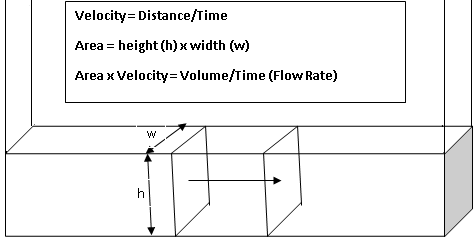
\includegraphics[scale=0.5]{ChannelFlow3}\\
$Q=V*A \implies V=\dfrac{Q}{A}$\\
$\implies V\dfrac{ft}{s}=\dfrac{3.5\dfrac{\cancel{MG}}{\cancel{day}}*\dfrac{1000000\cancel{gal}}{\cancel{MG}}*\dfrac{ft^{\cancel{3}}}{7.48\cancel{gal}}*\dfrac{\cancel{day}}{(1440*60)s}}{(3.25*0.75)\cancel{ft^2}}=\boxed{2.2\dfrac{ft}{s}}$

\item A plastic float is dropped into a wastewater channel and is found to travel 10 feet in 4.2 seconds. The channel is 2.4 feet wide and is flowing 1.8 feet deep. Calculate the flow rate of this wastewater in cubic feet per second.\\
Solution:\\
$Q=V*A$\\
$\implies Q\Big(\dfrac{ft^3}{s}\Big)=\dfrac{10ft}{4.2s}*(2.4*1.8)ft^2=\boxed{10.3\dfrac{ft^3}{s}}$
\item A 12 inch pipe conveys sewage at 2.6 feet per second.  What is the flow expressed in MGD?
Solution:\\
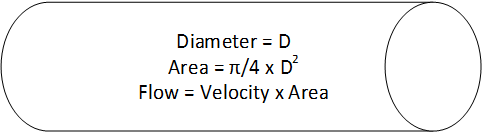
\includegraphics[scale=0.5]{PipeFlow}\\
$Q=V*A$\\
$Q=2.6\dfrac{\cancel{ft}}{\cancel{s}}*0.785*1^2\cancel{ft^2}*7.48\dfrac{\cancel{gal}}{ft^3}*\dfrac{MG}{1,000,000\cancel{gal}}*\dfrac{(1440*60)\cancel{s}}{day}=\boxed{1.3MGD}$\\

\item A sewer line to a wastewater treatment plant is 12 miles long. If the wastewater is flowing at 2.2 fps, approximately.  How long will it take for wastewater to reach the plant?\\
Solution:\\
$time \enspace to \enspace reach \enspace plant \enspace (hrs)=\dfrac{\cancel{s}}{2.2\cancel{ft}}*\dfrac{5280\cancel{ft}}{\cancel{mile}}*12\cancel{miles}*\dfrac{hrs}{(60*60)\cancel{s}}=\boxed{8hrs}$  
\end{enumerate}
\section{Preliminary Treatment}\index{Preliminary Treatment}
\begin{enumerate}
\item On an average a 12.5 yd. load of grit is hauled to the landfill once every 20 days. Plant flow averages 12.5 MGD. Calculate the rate of grit collection in ft$^3$/MG.\\
Solution:\\
$Grit Removal\Big(\dfrac{ft^3}{MG}\Big)=\dfrac{12.5\cancel{yd^3}}{ 20\cancel{days}}*\dfrac{27ft^3}{ \cancel{yd^3}}*\dfrac{\cancel{day}}{12.5MG}=\boxed{1.4\dfrac{ft^3}{MG}}$

\item On an average, 2 inches of grit is collected and removed every day in a 2.2 feet wide, 205 feet long grit channel.  Knowing the average flow through that grit channel is 10 MGD calculate the rate of grit collection in ft$^3$/MG\\
Solution:\\
Grit volume accumulated:  $\dfrac{2}{12}ft*(2.2*205)ft^2=\dfrac{75.16ft^3}{day}$
Grit Collection: $\dfrac{\dfrac{75.16ft^3}{\cancel{day}}}{\dfrac{10MG}{\cancel{day}}}=\boxed{7.5\dfrac{ft^3}{MG}}$ 
\end{enumerate}

\section{Primary Treatment} \index{Primary Treatment}
\begin{enumerate}
\item A circular clarifier receives a flow of 11 MGD.  If the clarifier is 90 ft. in diameter and is 12 ft. deep, what is: a) the hydraulic/surface loading rate, b) weir overflow rate, and c) clarifier detention time in hours?\\
Solution:\\
a) Hydraulic/surface loading rate:\\
$Clarifier \enspace hydraulic \enspace loading \enspace 	\Big(\dfrac{gpd}{ft^2}\Big) ==\dfrac{\dfrac{11\cancel{MG}}{{day}}*\dfrac{10^6gal}{\cancel{MG}}}{0.785*90^2 ft^2}=\boxed{1,730gpd/ft^2}$\\
b) Weir overflow rate:\\ 
$Weir \enspace overflow \enspace rate \Big(\dfrac{gpd}{ft}\Big) =\dfrac{\dfrac{11\cancel{MG}}{{day}}*\dfrac{10^6gal}{\cancel{MG}}}{3.14*90 ft}=\boxed{38,924gpd/ft}$\\
c) Clarifier detention time:\\
$Clarifier \enspace detention \enspace time \enspace (hr) = 	\dfrac{ Clarifier \enspace volume (cu.ft \enspace or \enspace gal)}{Influent \enspace flow \enspace (cu.ft \enspace or \enspace gal)/hr)}$\\
$Clarifier \enspace detention \enspace time \enspace (hr) = 	\dfrac{(0.785*90^2*15)\cancel{ft^3}}{\dfrac{11\cancel{MG}}{\cancel{day}}*\dfrac{10^6\cancel{gal}}{\cancel{MG}}*\dfrac{\cancel{ft^3}}{7.48\cancel{gal}}*\dfrac{\cancel{day}}{24hrs}}=\boxed{2hrs}$\\

\item At a 2.5 MGD wastewater treatment plant the primary clarifier has a detention time of 2 hours. How many gallons does this clarifier hold?\\

Solution:\\
\vspace{0.2cm}
$Clarifier \enspace detention \enspace time \enspace (hr) = 	\dfrac{ Clarifier \enspace volume (gal)}{Influent \enspace flow \enspace (gal/hr)}$\\
\vspace{0.2cm}
$ \implies Clarifier \enspace volume (gal)=Clarifier \enspace detention \enspace time \enspace (hr)*Influent \enspace flow \enspace (gal/hr)$\\
\vspace{0.2cm}
$ \implies Clarifier \enspace volume (gal)= \Big(2 \enspace hrs\Big)*\Big(2.5*10^6 \enspace \dfrac{gal}{day}*\dfrac{day}{24 \enspace hrs}\Big)=\boxed{208,333 \enspace gals}$\\

\end{enumerate}
\section{Pumping}\index{Pumping}
\begin{enumerate}
\item A sludge pump is set to pump 5 minutes each hour. It pumps at the rate of 35 gpm. How many gallons of sludge are pumped each day?\\
Solution:\\
$\dfrac{35 \enspace gal \enspace sludge}{\cancel{min}}*\dfrac{5 \enspace \cancel{min}}{\cancel{hr}} *\dfrac{24 \enspace \cancel{hr}}{day}=\boxed{\dfrac{4,200 \enspace gallons}{day}}$\\

\item A community has a total flow of 15 MGD which is passed through a primary treatment plant which removes 60\% of the TSS and 35\% of the BOD. The average strength of the influent is 400 mg/l TSS and 275 mg/l BOD. If the total solids of the raw sludge is 5\%, how many cu. ft of sludge is pumped daily?\\
Solution:\\
$lbs \enspace solids \enspace removed=(400*0.60)mg/l*15MGD*8.34=30,024lbs \enspace solids \enspace per \enspace day$
$$\dfrac{ft^3\enspace sludge}{day}= \dfrac{30,924 \enspace \cancel{lbs \enspace solids}}{day} * \dfrac{1 \enspace \cancel{lb \enspace sludge}}{0.05\enspace \cancel{lbs \enspace solids}}*\dfrac{\cancel{gal \enspace sludge}}{8.34\cancel{lb \enspace sludge}}*\dfrac{ft^3 \enspace sludge}{7.48 \enspace \cancel{gal}}=\boxed{9,626\dfrac{ft^3 \enspace sludge}{day}} $$

\item How many lbs of solids are removed daily by a primary clarifier treating a 6 MGD flow if the average influent TSS concentration is 300 mg/l and the clarifier TSS removal efficiency is 67\%?\\
Solution:\\
As the removal efficiency is 67\%, 0.67 * 300 mg/l = 201 mg/l solids are removed.\\
The total lbs removed can be calculated using the lbs formula.\\
$ \dfrac{lbs \enspace solids}{day}= 6 MGD* 201  \dfrac{mg \enspace  SS}{l}*8.34=\boxed{10,058 \dfrac{lbs \enspace solids}{day}}$
\end{enumerate}

%\chapterimage{Dewatering.jpg} % Chapter heading image

\chapter{Part I - Practice Math Problems Solutions}

\section{Unit Conversions}\index{Unit Conversions}
\begin{enumerate}
\item Given 1 ft = 30.48 cm and 5,280 ft = mile, convert 3 miles to cm\\
Solution:\\
$3 \enspace \cancel{miles} * \dfrac{5,280 \enspace \cancel{ft}}{\cancel{mile}}*\dfrac{30.48 \enspace cm}{\cancel{ft}}=\boxed{482,803 \enspace cm}$

\item The wastewater flow to a treatment plant has a velocity of 61 cm/s. What is this velocity expressed in ft/min. Given: 1 ft = 30.48 cm\\
Solution:\\
$61 \enspace \dfrac{\cancel{cm}}{\cancel{s}} * \dfrac{ft}{30.48 \enspace \cancel{cm}}* \dfrac{60 \enspace \cancel{s}}{min} =  \boxed{120 \enspace ft/min}$\\

\item As an operator of a wastewater plant you are treating a flow of 21 MGD, what is the flow in gallons per minute?\\
Solution:\\
$\dfrac{21 \cancel{MG}}{\cancel{day}}*\dfrac{1,000,000 \enspace gal}{\cancel{MG}}*\dfrac{\cancel{day}}{24*60 \enspace min}=\boxed{\dfrac{14,583 \enspace gal}{min}}$\\
\end{enumerate}

\newpage

\section{Area \& Volume}\index{Area \& Volume}
\begin{enumerate}

\item A cylindrical tank is 10 feet in diameter and 20 feet in height. 'What is the approximate capacity in liters?\\
Solution:\\

\begin{tikzpicture}
\draw (0,0) ellipse (2cm and 0.3cm);
\draw (0,-2.3) ellipse (2cm and 0.3cm);
\draw [-] (2,-2.3) -- (2,0);
\draw [<->] (-2,0) -- (2,0) node [midway, above=3mm] {\hspace{0.1cm}Diameter=10'}; 
\draw [<->] (2.5,-2.3) -- (2.5,0) node [midway, below] {\hspace{1.9cm}Height=20'};
%\draw [-] (0,-4) -- (2,-2.3);
%\draw [-] (0,-4) -- (-2,-2.3);
%\draw [-] (0,-4) -- (2,-2.3);
\draw [-] (-2,0) -- (-2,-2.3);
\end{tikzpicture}\\

$Volume=\dfrac{\pi}{4}D^2*H=0.785*10^2*20\cancel{ft^3}*7.48\dfrac{\cancel{gallons}}{\cancel{ft^3}}*3.78\dfrac{liters}{\cancel{gallons}}=\boxed{44,462 \enspace liters}$

\item What is the volume of water in a sedimentation basin 80 feet long, 28 feet wide and a 9.5 feet water depth? Give your answer in gallons.\\
Solution:\\
$Volume=80*28*9.5 \cancel{ft^3}*7.48\dfrac{gallons}{\cancel{ft^3}}=\boxed{159,174 \enspace gallons} $

\item How many gallons will 1,200 feet of 6-inch pipe hold?\\
Solution:\\
\begin{center}
\begin{tikzpicture}
\draw (0,0) ellipse (0.1cm and 0.3cm);
\draw (10,0) ellipse (0.1cm and 0.3cm);
\draw [-] (0,-0.29) -- (10,-0.29);
\draw [-] (0,0.29) -- (10,0.29);
\draw [<->] (10,-0.28) -- (10,0.28) node [midway, below=-3mm] {\hspace{2.6cm}Diameter=6"};
\draw [<->] (0,-.68) -- (10,-.68)node [midway, below] {\hspace{0.9cm}Length=1,200'};
\end{tikzpicture}
\end{center}
$Volume=\dfrac{\pi}{4}D^2*L=0.785*\Big(\dfrac{6}{12}\Big)^2*1200\cancel{ft^3}*7.48\dfrac{gallons}{\cancel{ft^3}}=\boxed{1,762 \enspace gallons}$

\item What is the surface area of a cylinder 80 ft diameter and 25 ft height?  Cylindrical part surface area only. Disregard the floor and roof areas.\\
Solution:\\
\begin{center}
\begin{tikzpicture}[mydashed/.style={dashed,dash phase=2pt}]
\draw (0,0) ellipse (2cm and 0.3cm) node [midway, above=-2.4mm] {};
\draw (0,-2.3) ellipse (2cm and 0.3cm) node [midway, below=2.05cm] {};
\draw [-] (2,-2.3) -- (2,0);
%\draw [<->] (-2,0) -- (2,0); 
\draw [<->] (2.5,-2.3) -- (2.5,0) node [midway, below] {\hspace{2.9cm}Height (h) = 25'};
\draw [<->] (-2,-0.4) -- (2,-0.4) node [midway, below=0.7mm] {\hspace{0.1cm}\small{Diameter (D)}=80'};
%\draw [-] (0,-4) -- (2,-2.3);
%\draw [-] (0,-4) -- (-2,-2.3);
%\draw [-] (0,-4) -- (2,-2.3);
\draw [-] (-2,0) -- (-2,-2.3) node [midway, below] {\hspace{4cm}\tiny{Cylinder Surface Area$=\pi*D*h$}};
\draw [-latex, mydashed, line width=1mm, rotate=-90] (0.6,-1.9) arc [start angle=-120, end angle=120, x radius=0.8cm, y radius=2.2cm];
%\draw [-latex, thick, rotate=-95] (0,0) arc [start angle=-190, end angle=160, x radius=1cm, y radius=2cm];
\end{tikzpicture}\\
\end{center}
$Surface \enspace area \enspace of \enspace cylinder=\pi*D*h=3.14*80*25=\boxed{6,280ft^2}$

\item If the surface area of a clarifier is 5,025$ft^2$, what is its circumference?\\
Solution:\\
$Surface \enspace area=\dfrac{\pi}{4}*D^2 \enspace \implies 5025ft^2=0.785*D^2 ft^2\implies D^2=\dfrac{5025}{0.785} \implies D=\sqrt{6401.3}=80ft \implies \enspace Circumference=\pi*D=3.14*80ft=\boxed{251ft}$

\item How many gallons of paint will be required to paint the inside walls of a 40 ft long x 65 ft wide x 20 ft high tank if the paint coverage is 150 sq. ft per gallon.  Note:  We are painting walls only.  Disregard the floor and roof areas.\\
Solution:\\
\begin{center}
\begin{tikzpicture}
	%%% Edit the following coordinate to change the shape of your
	%%% cuboid
      
	%% Vanishing points for perspective handling
	\coordinate (P1) at (-7cm,1.5cm); % left vanishing point (To pick)
	\coordinate (P2) at (8cm,1.5cm); % right vanishing point (To pick)

	%% (A1) and (A2) defines the 2 central points of the cuboid
	\coordinate (A1) at (0em,0cm); % central top point (To pick)
	\coordinate (A2) at (0em,-2cm); % central bottom point (To pick)

	%% (A3) to (A8) are computed given a unique parameter (or 2) .8
	% You can vary .8 from 0 to 1 to change perspective on left side
	\coordinate (A3) at ($(P1)!.8!(A2)$); % To pick for perspective 
	\coordinate (A4) at ($(P1)!.8!(A1)$);

	% You can vary .8 from 0 to 1 to change perspective on right side
	\coordinate (A7) at ($(P2)!.7!(A2)$);
	\coordinate (A8) at ($(P2)!.7!(A1)$);

	%% Automatically compute the last 2 points with intersections
	\coordinate (A5) at
	  (intersection cs: first line={(A8) -- (P1)},
			    second line={(A4) -- (P2)});
	\coordinate (A6) at
	  (intersection cs: first line={(A7) -- (P1)}, 
			    second line={(A3) -- (P2)});

	%%% Depending of what you want to display, you can comment/edit
	%%% the following lines

	%% Possibly draw back faces

	\fill[gray!40] (A2) -- (A3) -- (A6) -- (A7) -- cycle; % face 6
	\node at (barycentric cs:A2=1,A3=1,A6=1,A7=1) {};
	
	\fill[gray!50] (A3) -- (A4) -- (A5) -- (A6) -- cycle; % face 3
	\node at (barycentric cs:A3=1,A4=1,A5=1,A6=1) {\tiny Wall - W*H};
	
	\fill[gray!10, opacity=0.2] (A5) -- (A6) -- (A7) -- (A8) -- cycle; % face 4
	\node at (barycentric cs:A5=1,A6=1,A7=1,A8=1) {\tiny Wall - L*H};
	
	\fill[gray!10,opacity=0.5] (A1) -- (A2) -- (A3) -- (A4) -- cycle; % f2
	\node at (barycentric cs:A1=1,A2=1,A3=1,A4=1) {\tiny Wall - L*H};
	
	\fill[gray!40,opacity=0.2] (A1) -- (A4) -- (A5) -- (A8) -- cycle; % f5
	\node at (barycentric cs:A1=1,A4=1,A5=1,A8=1) {};	
	
	\draw[thick,dashed] (A5) -- (A6);
	\draw[thick,dashed] (A3) -- (A6);
	\draw[thick,dashed] (A7) -- (A6);

	%% Possibly draw front faces

	%\fill[orange] (A1) -- (A8) -- (A7) -- (A2) -- cycle; % face 1
	\node at (barycentric cs:A1=1,A8=1,A7=1,A2=1) {\tiny Wall - W*H};
	


	%% Possibly draw front lines
	\draw[thick] (A1) -- (A2);

	\draw[<->] (-1.8,0.38) -- (-1.8,-1.3)node [midway, above=-1.8mm] {\hspace{-1.3cm}\tiny Height=20'};
	\draw[<->] (-1.6,-1.4) -- (-.3,-2.1)node [midway, above=-2.6mm] {\hspace{-1.3cm}\tiny Length=45'};
	\draw[<->] (2.6,-1.13) -- (0.2,-2.2)node [midway, below=.6mm] {\hspace{1.2cm}\tiny Width=65'};
	\draw[thick] (A3) -- (A4);
	\draw[thick] (A7) -- (A8);
	\draw[thick] (A1) -- (A4);
	\draw[thick] (A1) -- (A8);
	\draw[thick] (A2) -- (A3);
	\draw[thick] (A2) -- (A7);
	\draw[thick] (A4) -- (A5);
	\draw[thick] (A8) -- (A5);
	
	% Possibly draw points
	% (it can help you understand the cuboid structure)
%	\foreach \i in {1,2,...,8}
%	{
%	  \draw[fill=black] (A\i) circle (0.15em)
%	    node[above right] {\tiny \i};
%	}
	% \draw[fill=black] (P1) circle (0.1em) node[below] {\tiny p1};
	% \draw[fill=black] (P2) circle (0.1em) node[below] {\tiny p2};
\end{tikzpicture}\\
\end{center}
2 Walls W*H + 2 Walls L*H = $2*65*20ft^2 + 2*40*20ft^2= 2,600+1,600=4,200ft^2$\\
$\implies @150\dfrac{ft^2}{gal} \enspace paint \enspace coverage \enspace \rightarrow \enspace \dfrac{4,200\cancel{ft^2}}{150\dfrac{\cancel{ft^2}}{gal}}=\boxed{28 \enspace gallons}$

\item What is the circumference of a 100 ft diameter circular clarifier?\\
Solution:\\
$Circumference=\pi*D=3.14*100ft=\boxed{314ft}$

\item If the surface area of a clarifier is 5,025$ft^2$, what is its diameter?\\
Solution:\\
$Surface \enspace area=\dfrac{\pi}{4}*D^2 \enspace \implies 5025ft^2=0.785*D^2 ft^2\implies D^2=\dfrac{5025}{0.785} \implies D=\sqrt{6401.3}=\boxed{80ft}$

\end{enumerate}

\section{Concentration}\index{Concentration}
\begin{enumerate}
\item A 6.35\% solution is is equivalent to {\underline{\hspace{1cm}}} mg/l\\
Answer:\\
63,500 mg/l\\
\end{enumerate}
\section{Pounds Formula}\index{Pounds Formula}
\begin{enumerate}
\item An operator dissolves 1,200 lbs of a chemical in 12,000 gallons of water, what is the resultant concentration in mg/l, of the chemical solution?\\
Solution:\\
$Concentration \enspace \dfrac{mg}{l}=\dfrac{lbs}{Volume \enspace MG \enspace * \enspace 8.34}$\\
$Concentration \enspace \dfrac{mg}{l}=\dfrac{1,200}{0.012 \enspace * \enspace 8.34}=\boxed{\dfrac{11,990 \enspace mg}{l} \enspace or \enspace 1.2\% \enspace solution}$\\
\textbf{Note:}\\  
12,000 gallons was converted to MG by dividing by 1,000,000\\
$12,000 \enspace gallons * \dfrac{1 MG}{1,000,000 \enspace gallons}$\\
\end{enumerate}
\section{Removal Efficiency}\index{Removal Efficiency}
\begin{enumerate}

\item What is the \% removal efficiency if the influent concentration is 10 mg/L and the effluent concentration is 2.5 mg/L?\\
$Removal \enspace Rate (\%) = \dfrac{In-Out}{In}*100 \implies \dfrac{10-2.5}{10}*100=\boxed{75\%}$

\item If a plant removes 35\% of the influent BOD in the primary treatment and 85\% of the remaining BOD in the secondary system, what is the BOD of the raw wastewater if the BOD of the final effluent is 20mg/l \\
Solution:\\
\tikzstyle{block} = [rectangle, draw, fill=red!40, 
    text width=6em, text centered, rounded corners, minimum height=3em]
\tikzstyle{arrow} = [draw, -latex']
\begin{figure}[!h]
\centering
\begin{tikzpicture}[node distance =1.5cm, auto]
    \draw ++(0,0) node [block] (Primary) {Primary};
    
   \node[node distance=1.9in] (dummy_in) [left of=Primary] {Influent BOD};
   \node[node distance=1.9in] (dummy_out) [right of=Primary] {Primary BOD Out};
	\node (Removal) [below of=Primary, yshift=-0in] {$Removal \enspace Efficiency=35\% $};
    \path [arrow] (dummy_in)-- (Primary)  node [above] {\hspace{-4.8cm}$X \enspace mg/l \enspace$} node [below] {};
    \path [arrow] (Primary) -- (dummy_out)  node [above] {\hspace{-4.9cm}$0.65X \enspace mg/l$} node [below] {};
   \draw[arrow] (Process) -- (Removal);
\end{tikzpicture}
\end{figure}

\tikzstyle{block} = [rectangle, draw, fill=red!40, 
    text width=6em, text centered, rounded corners, minimum height=3em]
\tikzstyle{arrow} = [draw, -latex']
\begin{figure}[!h]
\centering
\begin{tikzpicture}[node distance =1.5cm, auto]
    \draw ++(0,0) node [block] (Secondary) {Secondary};
    
   \node[node distance=1.9in] (dummy_in) [left of=Secondary] {Primary BOD Out};
   \node[node distance=1.9in] (dummy_out) [right of=Secondary] {Secondary BOD Out};
	\node (Removal) [below of=Secondary, yshift=-0in] {$Removal \enspace Efficiency=85\% $};
    \path [arrow] (dummy_in)-- (Secondary)  node [above] {\hspace{-4.8cm}$0.65X \enspace mg/l \enspace$} node [below] {\hspace{-5cm}$100 \enspace mg/l$};
    \path [arrow] (Secondary) -- (dummy_out)  node [above] {\hspace{-4.9cm}$20 \enspace mg/l$} node [below] {\hspace{-4.9cm}$15 \enspace mg/l$};
   \draw[arrow] (Process) -- (Removal);
\end{tikzpicture}
\end{figure}
\vspace{0.3cm}
For the Secondary process:\\
$\dfrac{In}{Out}: \enspace \dfrac{0.65X}{20}=\dfrac{100}{15} \implies X \enspace mg/l=\dfrac{100*20}{15*0.65}=\boxed{205 \enspace mg/l}$\\

\vspace{0.3cm}
Alternate Solution \#1

$\xrightarrow[
				\text{X}\dfrac{mg}{l}
			]
			{
			\text{Influent BOD}
			}
 \boxed{Primary}
 \xrightarrow[
 				\text{X-0.35X=X*(1-0.35)=0.65X}\dfrac{mg}{l}
 			]
 			{
 			\text{Primary Effluent BOD}
 			}
 \boxed{Secondary}
 \xrightarrow[
				\text{0.65X-0.5525X=(0.65-0.5525)X=0.0975X }
			 ]
			{
			\text{Secondary Effluent BOD}
			}
$\\

\hspace{2.8cm}$\downarrow$ {\tiny(0.35X)BOD Removed}\hspace{3.2cm}$\downarrow$ {\tiny(0.65*0.85)X = 0.5525X BOD Removed}\\
$\implies 0.0975X=20 \implies X=\dfrac{20}{0.0975}=\boxed{205\dfrac{mg}{l}}$\\

\vspace{0.3cm}

Alternate Solution \#2:\\
$\xrightarrow[\text{X}\dfrac{mg}{l}]{\text{Influent BOD}}\boxed{Primary}\xrightarrow[\text{0.65X}]{\text{Primary Effluent BOD}}\boxed{Secondary}\xrightarrow[\text{(0.65*0.15)X}]{\text{Secondary Effluent BOD}}$\\
\hspace{2.8cm}$\downarrow$ {\tiny(0.35X)BOD Removed}\hspace{2.2cm}$\downarrow$ {\tiny(0.65X*0.85)BOD Removed}\\

Primary Effluent BOD = Influent BOD * (1-Primary BOD Removal), and\\
Secondary Effluent BOD=[Primary Effluent BOD]*(1-Secondary BOD Removal)\\
Secondary Eff. BOD=[Influent BOD * (1-Primary BOD Removal)]*(1-Secondary BOD Removal)\\

Therefore, 20 = [X*(1-0.35)] * (1-0.85)= X*0.65*0.15\\
$\implies 20 \enspace \dfrac{mg}{l}= 0.0975X \implies X=\dfrac{20}{0.0975}=\boxed{205 \enspace \dfrac{mg}{l}}$\\

\item Calculate the inlet concentration if the outlet concentration is 80 mg/l and the process removal efficiency is 60\%\\

\tikzstyle{block} = [rectangle, draw, fill=red!40, 
    text width=6em, text centered, rounded corners, minimum height=3em]
\tikzstyle{arrow} = [draw, -latex']
\begin{figure}[!h]
\centering
\begin{tikzpicture}[node distance =1.5cm, auto]
    \draw ++(0,0) node [block] (Process) {Process};
   \node[node distance=1.5in] (dummy_in) [left of=Process] {In};
   \node[node distance=1.5in] (dummy_out) [right of=Process] {Out};
	\node (Removal) [below of=Process, yshift=-0in] {$Removal \enspace Efficiency=60\%$};
    \path [arrow] (dummy_in)-- (Process)  node [above] {\hspace{-4.39cm}$Xmg/l$} node [below] {\hspace{-4.39cm}$100mg/l$};
    \path [arrow] (Process) -- (dummy_out)  node [above] {\hspace{-3.cm}80mg/l} node [below] {\hspace{-3cm}40mg/l};
   \draw[arrow] (Process) -- (Removal);
\end{tikzpicture}
\end{figure}

$\dfrac{In}{Out} \enspace : \enspace \dfrac{Actual \enspace inlet \enspace  (X)}{80}=\dfrac{100}{100-60}$\\
$\implies \dfrac{Actual \enspace inlet \enspace  (X)}{80}=2.5$\\    
Rearranging the equation:   $Actual \enspace inlet (X)=2.5*80 = \boxed{200 mg/l}$\\

\item Calculate the outlet concentration if the inlet concentration is 80 mg/l and the process removal efficiency is 60\%\\
Solution:\\

\tikzstyle{block} = [rectangle, draw, fill=red!40, 
    text width=6em, text centered, rounded corners, minimum height=3em]
\tikzstyle{arrow} = [draw, -latex']
\begin{figure}[!h]
\centering
\begin{tikzpicture}[node distance =1.5cm, auto]
    \draw ++(0,0) node [block] (Process) {Process};
   \node[node distance=1.5in] (dummy_in) [left of=Process] {In};
   \node[node distance=1.5in] (dummy_out) [right of=Process] {Out};
	\node (Removal) [below of=Process, yshift=-0in] {$Removal \enspace Efficiency=60\%$};
    \path [arrow] (dummy_in)-- (Process)  node [above] {\hspace{-4.39cm}$80mg/l$} node [below] {\hspace{-4.39cm}$100mg/l$};
    \path [arrow] (Process) -- (dummy_out)  node [above] {\hspace{-3.cm}$Xmg/l$} node [below] {\hspace{-3cm}40mg/l};
   \draw[arrow] (Process) -- (Removal);
\end{tikzpicture}
%\caption[MFCC]{Diagrama en bloques del cálculo de las MFCC para un frame.}
%\label{MFCC}
\end{figure}
\vspace{0cm}
$\dfrac{Out}{In} \enspace:\enspace\dfrac{Actual \enspace Outlet (X)}{80}=\dfrac{100-60}{100}$\\
$\implies \dfrac{Actual \enspace Outlet (X)}{80} =0.4$\\
$\implies Actual \enspace  Outlet (X) = 0.4 * 80 = \boxed{32 mg/l}$\\

\end{enumerate}

\section{Flow and Velocity}\index{Flow and Velocity}
\begin{enumerate}
\item A wastewater channel is 3.25 feet wide and is conveying a wastewater flow of 3.5 MGD. The wastewater flow is 8 inches deep. Calculate the velocity of this flow.\\
Solution:\\
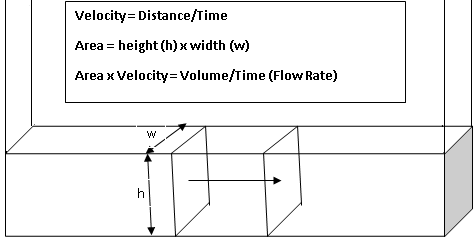
\includegraphics[scale=0.5]{ChannelFlow3}\\
$Q=V*A \implies V=\dfrac{Q}{A}$\\
$\implies V\dfrac{ft}{s}=\dfrac{3.5\dfrac{\cancel{MG}}{\cancel{day}}*\dfrac{1000000\cancel{gal}}{\cancel{MG}}*\dfrac{ft^{\cancel{3}}}{7.48\cancel{gal}}*\dfrac{\cancel{day}}{(1440*60)s}}{(3.25*0.75)\cancel{ft^2}}=\boxed{2.2\dfrac{ft}{s}}$

\item A plastic float is dropped into a wastewater channel and is found to travel 10 feet in 4.2 seconds. The channel is 2.4 feet wide and is flowing 1.8 feet deep. Calculate the flow rate of this wastewater in cubic feet per second.\\
Solution:\\
$Q=V*A$\\
$\implies Q\Big(\dfrac{ft^3}{s}\Big)=\dfrac{10ft}{4.2s}*(2.4*1.8)ft^2=\boxed{10.3\dfrac{ft^3}{s}}$
\item A 12 inch pipe conveys sewage at 2.6 feet per second.  What is the flow expressed in MGD?
Solution:\\
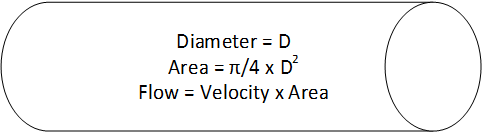
\includegraphics[scale=0.5]{PipeFlow}\\
$Q=V*A$\\
$Q=2.6\dfrac{\cancel{ft}}{\cancel{s}}*0.785*1^2\cancel{ft^2}*7.48\dfrac{\cancel{gal}}{ft^3}*\dfrac{MG}{1,000,000\cancel{gal}}*\dfrac{(1440*60)\cancel{s}}{day}=\boxed{1.3MGD}$\\

\item A sewer line to a wastewater treatment plant is 12 miles long. If the wastewater is flowing at 2.2 fps, approximately.  How long will it take for wastewater to reach the plant?\\
Solution:\\
$time \enspace to \enspace reach \enspace plant \enspace (hrs)=\dfrac{\cancel{s}}{2.2\cancel{ft}}*\dfrac{5280\cancel{ft}}{\cancel{mile}}*12\cancel{miles}*\dfrac{hrs}{(60*60)\cancel{s}}=\boxed{8hrs}$  
\end{enumerate}
\section{Preliminary Treatment}\index{Preliminary Treatment}
\begin{enumerate}
\item On an average a 12.5 yd. load of grit is hauled to the landfill once every 20 days. Plant flow averages 12.5 MGD. Calculate the rate of grit collection in ft$^3$/MG.\\
Solution:\\
$Grit Removal\Big(\dfrac{ft^3}{MG}\Big)=\dfrac{12.5\cancel{yd^3}}{ 20\cancel{days}}*\dfrac{27ft^3}{ \cancel{yd^3}}*\dfrac{\cancel{day}}{12.5MG}=\boxed{1.4\dfrac{ft^3}{MG}}$

\item On an average, 2 inches of grit is collected and removed every day in a 2.2 feet wide, 205 feet long grit channel.  Knowing the average flow through that grit channel is 10 MGD calculate the rate of grit collection in ft$^3$/MG\\
Solution:\\
Grit volume accumulated:  $\dfrac{2}{12}ft*(2.2*205)ft^2=\dfrac{75.16ft^3}{day}$
Grit Collection: $\dfrac{\dfrac{75.16ft^3}{\cancel{day}}}{\dfrac{10MG}{\cancel{day}}}=\boxed{7.5\dfrac{ft^3}{MG}}$ 
\end{enumerate}

\section{Primary Treatment} \index{Primary Treatment}
\begin{enumerate}
\item A circular clarifier receives a flow of 11 MGD.  If the clarifier is 90 ft. in diameter and is 12 ft. deep, what is: a) the hydraulic/surface loading rate, b) weir overflow rate, and c) clarifier detention time in hours?\\
Solution:\\
a) Hydraulic/surface loading rate:\\
$Clarifier \enspace hydraulic \enspace loading \enspace 	\Big(\dfrac{gpd}{ft^2}\Big) ==\dfrac{\dfrac{11\cancel{MG}}{{day}}*\dfrac{10^6gal}{\cancel{MG}}}{0.785*90^2 ft^2}=\boxed{1,730gpd/ft^2}$\\
b) Weir overflow rate:\\ 
$Weir \enspace overflow \enspace rate \Big(\dfrac{gpd}{ft}\Big) =\dfrac{\dfrac{11\cancel{MG}}{{day}}*\dfrac{10^6gal}{\cancel{MG}}}{3.14*90 ft}=\boxed{38,924gpd/ft}$\\
c) Clarifier detention time:\\
$Clarifier \enspace detention \enspace time \enspace (hr) = 	\dfrac{ Clarifier \enspace volume (cu.ft \enspace or \enspace gal)}{Influent \enspace flow \enspace (cu.ft \enspace or \enspace gal)/hr)}$\\
$Clarifier \enspace detention \enspace time \enspace (hr) = 	\dfrac{(0.785*90^2*15)\cancel{ft^3}}{\dfrac{11\cancel{MG}}{\cancel{day}}*\dfrac{10^6\cancel{gal}}{\cancel{MG}}*\dfrac{\cancel{ft^3}}{7.48\cancel{gal}}*\dfrac{\cancel{day}}{24hrs}}=\boxed{2hrs}$\\

\item At a 2.5 MGD wastewater treatment plant the primary clarifier has a detention time of 2 hours. How many gallons does this clarifier hold?\\

Solution:\\
\vspace{0.2cm}
$Clarifier \enspace detention \enspace time \enspace (hr) = 	\dfrac{ Clarifier \enspace volume (gal)}{Influent \enspace flow \enspace (gal/hr)}$\\
\vspace{0.2cm}
$ \implies Clarifier \enspace volume (gal)=Clarifier \enspace detention \enspace time \enspace (hr)*Influent \enspace flow \enspace (gal/hr)$\\
\vspace{0.2cm}
$ \implies Clarifier \enspace volume (gal)= \Big(2 \enspace hrs\Big)*\Big(2.5*10^6 \enspace \dfrac{gal}{day}*\dfrac{day}{24 \enspace hrs}\Big)=\boxed{208,333 \enspace gals}$\\

\end{enumerate}
\section{Pumping}\index{Pumping}
\begin{enumerate}
\item A sludge pump is set to pump 5 minutes each hour. It pumps at the rate of 35 gpm. How many gallons of sludge are pumped each day?\\
Solution:\\
$\dfrac{35 \enspace gal \enspace sludge}{\cancel{min}}*\dfrac{5 \enspace \cancel{min}}{\cancel{hr}} *\dfrac{24 \enspace \cancel{hr}}{day}=\boxed{\dfrac{4,200 \enspace gallons}{day}}$\\

\item A community has a total flow of 15 MGD which is passed through a primary treatment plant which removes 60\% of the TSS and 35\% of the BOD. The average strength of the influent is 400 mg/l TSS and 275 mg/l BOD. If the total solids of the raw sludge is 5\%, how many cu. ft of sludge is pumped daily?\\
Solution:\\
$lbs \enspace solids \enspace removed=(400*0.60)mg/l*15MGD*8.34=30,024lbs \enspace solids \enspace per \enspace day$
$$\dfrac{ft^3\enspace sludge}{day}= \dfrac{30,924 \enspace \cancel{lbs \enspace solids}}{day} * \dfrac{1 \enspace \cancel{lb \enspace sludge}}{0.05\enspace \cancel{lbs \enspace solids}}*\dfrac{\cancel{gal \enspace sludge}}{8.34\cancel{lb \enspace sludge}}*\dfrac{ft^3 \enspace sludge}{7.48 \enspace \cancel{gal}}=\boxed{9,626\dfrac{ft^3 \enspace sludge}{day}} $$

\item How many lbs of solids are removed daily by a primary clarifier treating a 6 MGD flow if the average influent TSS concentration is 300 mg/l and the clarifier TSS removal efficiency is 67\%?\\
Solution:\\
As the removal efficiency is 67\%, 0.67 * 300 mg/l = 201 mg/l solids are removed.\\
The total lbs removed can be calculated using the lbs formula.\\
$ \dfrac{lbs \enspace solids}{day}= 6 MGD* 201  \dfrac{mg \enspace  SS}{l}*8.34=\boxed{10,058 \dfrac{lbs \enspace solids}{day}}$
\end{enumerate}



\part{Part II}
\chapterimage{Dewatering.jpg} % Chapter heading image

\chapter{Theory Part II}

\section{Secondary Treatment}\index{Secondary Treatment}
\begin{itemize}
\item While preliminary and primary treatment processes are designed primarily to remove solids from wastewater, secondary treatment is for the removal of organics.
\item Secondary treatment involves:
\begin{itemize}
\item biological conversion of the dissolved and suspended organics in wastewater into biomass, and
\item physical settling (separation) process where the solids including the biomass formed during secondary treatment is separated and removed from the treated wastewater.
\end{itemize}

\item With the removal of gross solids in the preliminary treatment followed by removable of settleable solids in the primary clarifiers and the removal of dissolved and suspended organics in the secondary treatment processes, the wastewater is considered treated.
\item Secondary treated wastewater is typically disposed or treated further for reuse or disposal (depending upon the end use/application and the NPDES permit stipulations).
\item The solids (biomass) removed from the secondary treatment is typically mixed with the solids from primary treatment and stabilized using a solids treatment process like sludge digestion prior to its disposal.
\end{itemize}
\vspace{1cm}

\textbf{Secondary treatment process incorporates one of the following three approaches:}


\subsection{Fixed film system}\index{Fixed Film System}	
		
Trickling filter is a fixed film secondary treatment process wherein the organic content of the wastewater is removed using biological growth attached to an inert media such as lava rock or plastic\\
\begin{center}
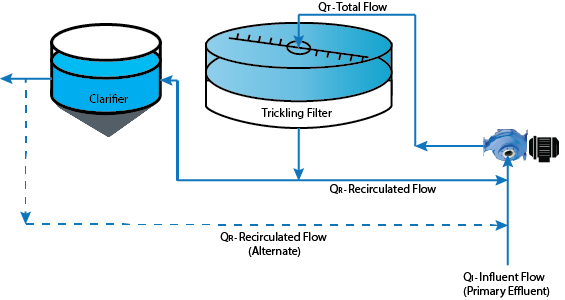
\includegraphics[scale=0.5]{TricklingFilter}
\end{center}		
\begin{itemize}
\item In a trickling filter, the wastewater is sprayed evenly on the surface of the media with a rotary type distributor with orifices
\item The wastewater percolates through the media bed, where it comes in contact with biological slime growth – zoogleal film (zooglea)
\item The aerobic biomass - bacteria, protozoa and other microoorganisms in the zooglea capture and consume the suspended and dissolved organics from the wastewater.
\item The microorganisms metabolize the organics and in the process produce more microbial mass resulting in increasing the thickness of the zoogleal layer.
\item The thickness of the zoogleal layer can only increase to a point until the wastewater flow – hydraulic load, shears the slime layer – “sloughs off” and is carried out as part of the effluent flow as sloughing.
\item The treated wastewater cascades from the bottom of the media into the underdrain system – lower portion of the TF comprised of columns which support the media base.  The underdrain has a sloping floor to direct the cascading water into a center channel .
\item The clarifier allows for the separation (settling) of the  of the solids (sloughed off material).  The settled solids is removed - typically pumped to a digester and the clarified effluent flows out of the clarifier.
\item The source of oxygen to support the aerobic growth is from the oxygen dissolved in the wastewater as it is sprayed over the media and from the air currents due to the downward flow of the wastewater and the temperature difference between ambient and the interior of the trickling filter.  Forced ventilation system may be designed as part of the trickling filter

\item Word trickling “filter” is a misnomer - no filtration is involved
\item Advantage includes process simplicity and lower costs
\item Disadvantage include BOD removal efficiency of only about 80-85%
\item The media may be rock, slag, coal, bricks, redwood blocks, molded plastic, or any other sound durable material.
\item The media depth ranges from about three to eight feet for rock media trickling filters and 15 to 30 feet for synthetic media.
\item The media needs to be uniformly sized and have adequate empty spaces (voids) to ensure maintaining aerobic condition necessary for the survival of biomass.  

\item Pre-fabricated (synthetic) media - similar to the one shown below, has an advantage over the "dumped" type media such as lava rock of providing a greater surface area per volume upon which the zoologeal film may grow while providing ample void space for the free circulation of air.

\item Sometimes, due to inadequate hydraulic loading, portions of the zoogleal layer may become too thick and oxygen cannot penetrate its full depth, causing odor issues.





\end{itemize}



\subsection{Suspended Growth System}\index{Suspended Growth System}
\begin{itemize}
\item In this type of secondary treatment, the microbes are suspended in the
wastewater flow being treated. 
\item Air or oxygen is supplied to maintain an aerobic environment and to keep the microorganisms in suspension. 
\item Example of this secondary treatment approach include the activated sludge treatment process 
\end{itemize}

\subsubsection{Elements of Activated Sludge Process}\index{Elements of Activated Sludge Process}

\begin{center}
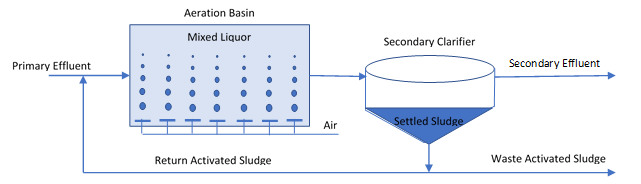
\includegraphics[height=4.5cm]{ASProcess}
\end{center}
\begin{itemize}

\item Utilizes an aeration basin/reactor and a secondary clarifier

\item In the presence of oxygen, aerobic bacteria in the aeration basin consume the organic matter (BOD) in wastewater for their growth and reproduction, converting BOD into bacterial cell mass along with metabolic byproducts including carbon dioxide and water

\item The aerobic bacteria is the predominant microbial life form in the aeration basin.  Other higher microbial life forms — mainly protozoa, are present along with some metazoans.

\item The microorganisms along with their metabolic byproducts and residual dead cell mass form a cluster called floc.

\item The wastewater exiting the aeration basin enters a clarifier where the floc settles.  The clear, treated secondary effluent flows out.

\item A portion of the settled activated sludge floc, is returned from the clarifier to the front of the aeration basin to seed the activated sludge treatment of the incoming primary effluent. The recycled floc is called \textbf{Return Activated Sludge (RAS)}.

\item The remaining settled floc from the clarifier is ”wasted” \textemdash transferred for solids treatment (typically using digestion) prior to its ultimate disposal. The wasted floc is called \textbf{Waste Activated Sludge (WAS)}.

\item The color of healthy activated sludge is tan to brown with an earthy/musty odor.

\item For activated sludge treatment to be effective, it is critical to establish a healthy microbial population which \hl{converts the BOD} into \hl{easily separable biomass.}
\item If the biomass does not settle well in the clarifier, it will be carried out in the treated secondary effluent producing a poor quality effluent with higher solids and organic content.  \\
\end{itemize}


\subsection{Pond System}\index{Pond System}
Similar to the suspended growth, stabilization ponds are large man made bodies of water which treat wastewater using mainly natural processes including sunlight, algae and microorganisms.
\begin{itemize}
\item Stabilization ponds and lagoons are bodies of water which treat wastewater using mainly natural processes including sunlight, algae and microorganisms for treating wastewater\\
\item While ponds are shallow and man-made, lagoons are bodies of water confined within natural boundaries.\\
\end{itemize}

 , which break down the effluent. It is in the anaerobic pond that the influent begins breaking down in the absence of oxygen "anaerobically". The anaerobic pond acts like an uncovered septic tank. Anaerobic bacteria break down the 

\subsubsection{Anaerobic Ponds}\index{Anaerobic Ponds}	

\begin{itemize}	
\item Typically for treating raw sewage
\item These are deep - 10-14 feet treatment ponds which rely primarily on anaerobic bacteria to break down the organic waste.
\item Designed for BOD removal
\item High strength wastewater may be treated.
\item Organic matter is broken down releasing releasing methane, carbon dioxide and odorous gases including hydrogen sulfide. 
\item Most of the decomposition is accomplished by acid forming bacteria. 
\item The pH in these lagoons is usually below 6.5. 
\item They are total retention and do not have an effluent discharge. 
\item The anaerobic pond must be de-sludged approximately once every 2 to 5 years
\item Organic loading of 200-1000 lbs. $BOD_5$ per acre per day
\end{itemize}

\subsubsection{Facultative Ponds}\index{Facultative Ponds}	

\begin{itemize}
\item The depth of facultative ponds is about 4-7 feet which is in-between the depths of anaerobic ponds (10-14 feet) and aerobic ponds 3 feet)
\item The uper layer of facultative pond is aerobic, and bottom layer is mostly anaerobic.
\item Facultative bacteria are responsible for most of the treatment that occurs in these ponds.  Facultative bacteria are bacteria which can live under both aerobic and anaerobic conditions.
\item The algae that grow in the pond are critical to the successful stabilization of the organic load. 
\item The algae will take in carbon dioxide ($CO_2$) and, through photosynthesis, use it to create sugars and release dissolved oxygen ($O_2$) that is used by the aerobic bacteria. Facultative lagoon levels should always maintain at least 4 feet of water in the pond.
\item Typically for secondary treatment - BOD removal
\item 15-50 lbs $BOD_5$ per acre per day.
\item Unused CO$_2$ will react with water to form carbonic acid - which would reduce the pH unless consumed
\item Sludge removal need is rare.  Sludge can be removed by using a raft-mounted sludge pump or by draining and dewatering the pond and removing the sludge with a front-end loader.
\end{itemize} 

				\begin{sidewaysfigure}
\begin{center}
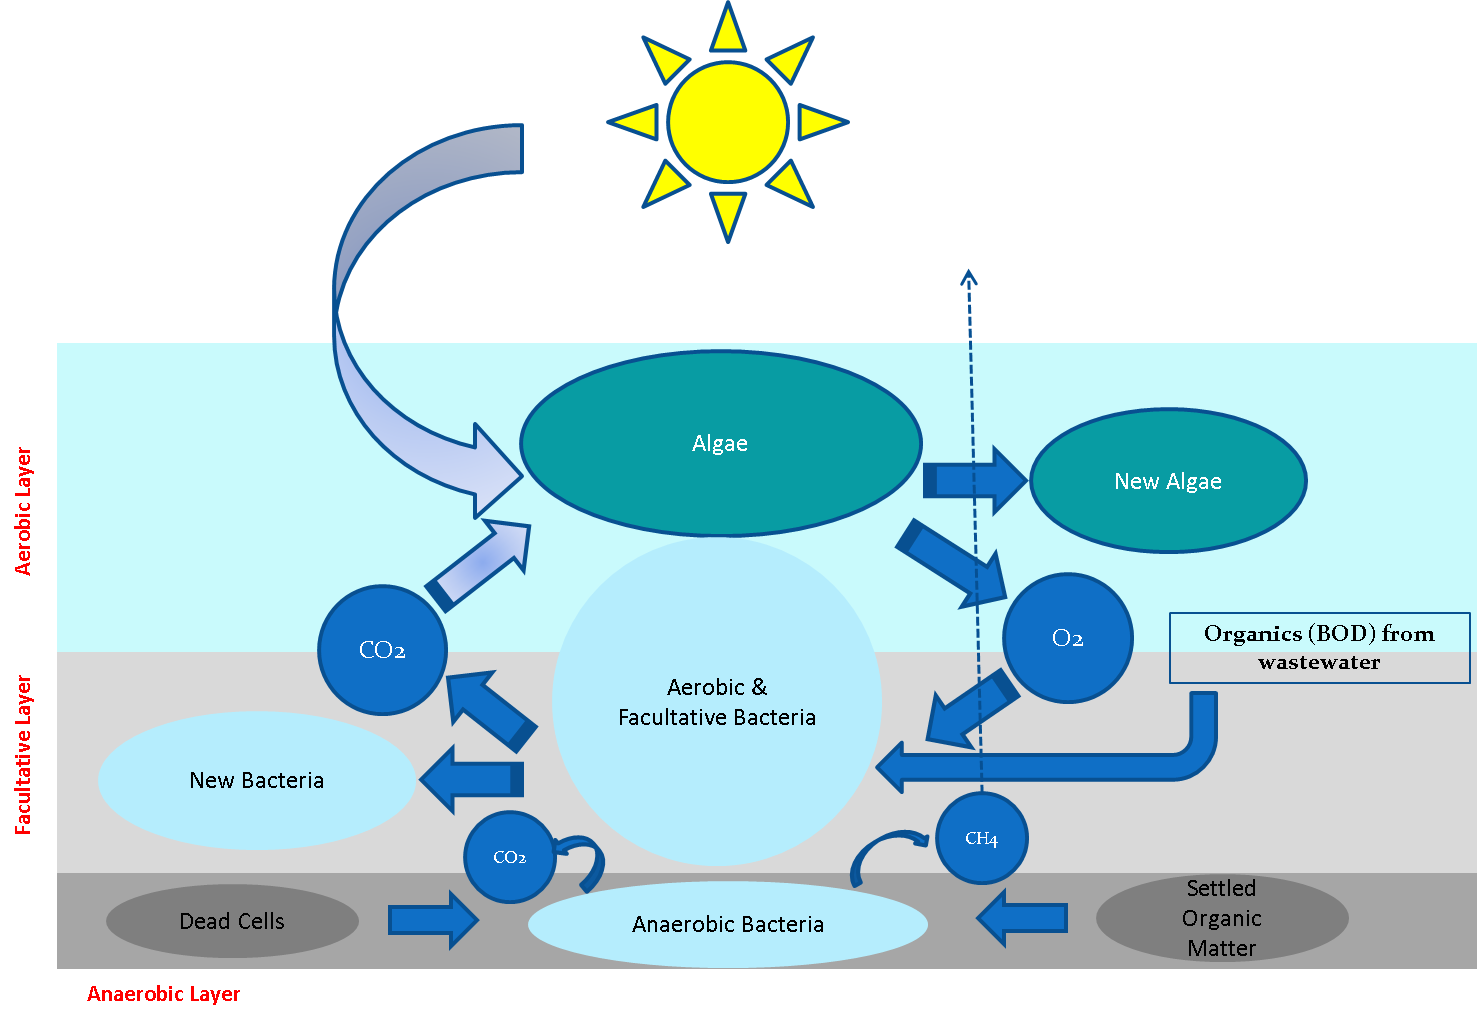
\includegraphics[scale=0.8]{StabilizationPond}\\
Facultative pond schematic
\end{center}
				\end{sidewaysfigure}
				
\subsubsection{Aerobic Stabilization Ponds}\index{Aerobic Stabilization Ponds}
	
Aerobic stabilization ponds are also known as: \hl{maturation}, \hl{polishing} or \hl{finishing} Pond
\begin{itemize}
\item Contain disssolved oxygen throughout entire depth of the pond.
\item Treatment is accomplished through the stabilization of organic wastes by aerobic bacteria and algae.
\item Typically for tertiary treatment
\item Designed for pathogen removal
\item Shallow - only about 3 feet deep. 
\item They are most often the final cells in a multi-staged pond system
\item They are also used as polishing ponds for tertiary treatment of trickling filter plant effluent.
\item Usually the effluent is directed into a second pond where the sludge can settle 
\item Their shallow depth allows sunlight to penetrate to the bottom of the pond to encourage algae growth and aerobic conditions throughout the pond 
\item The low solids loading found in these tertiary treatment applications means that these ponds normally have no sludge zone
\item These ponds may be mechanically aerated 
\item Aerobic polishing ponds are designed for 15-20 pounds BOD/acre/day
\item Aerobic ponds are typically designed for pathogen removal
\item Aerobic lagoon levels should always maintain at least 18 inches of water in the pond
\end{itemize}









\section{Solids Treatment}\index{Solids Treatment}




\subsection{Why do we need to treat wastewater solids?}\index{Why do we need to treat wastewater solids?}

\begin{itemize}
\item Sludge is generated from the wastewater treatment processes -  settled solids and scum from primary and secondary treatment processes
\item This sludge contain organic compounds and also elements that are beneficial plant nutrients
\item However, the organic solids in the sludge are not stable (i.e. they will decay) and include pathogens.  \item Prior to disposal, sludge has to be treated – stabilized, so that its disposal or reuse does not pose a threat to public health.
\item Sludge treatment is very critical as it is an expensive process and sludge disposal is subject to strict regulatory requirement.
\item Even solids are only a small component of wastewater, the solids treatment and disposal account for a very substantial portion of wastewater treatment costs.  Typically 40 to 60\% of total wastewater treatment operations cost is attributable to sludge treatment and disposal.
\end{itemize}

\textbf{NOTE: Solids removed during Preliminary Treatment, from barscreens and grit chambers are typically not treated as part of the solids treatment process.  These solids are disposed off at a landfill}

\vspace{0.5cm}
\textbf{Typical solids treatment is comprised of the following three sequential steps:
\begin{enumerate}
\item Sludge thickening
\item Sludge stabilization
\item Sludge dewatering
\end{enumerate}}
\vspace{0.5cm}

\subsection{Sludge thickening}\index{Sludge thickening}
Sludge thickening involves the removal of excess water from the primary and secondary sludge increasing the solids content of the sludge and reducing the volume of sludge to be treated in the sludge stabilization process.
Sludge thickening reduces the volume of sludge that need to be handled in the sludge stabilization step thereby reducing treatment cost.  
\begin{itemize}
\item There is an upper limit of the solids concentration that can be effectively treated (stabilized) as increasing the solids concentration reduces its ability to be mixed and pumped easily.  Typically the sludge thickening process produces sludge with a solids content of less than 10\%.\\
\end{itemize}
Benefits of thickening to the sludge stabilization process include:
\begin{itemize}
\item Improved performance due to a lower volume of sludge
\item Cost savings in the construction of new facilities
\item Reduction in energy requirements as less water has to be heated
\end{itemize}
Typical methods used for sludge thickening include:
\begin{enumerate}
\item Gravity thickener - more suitable for primary sludge
\item Dissolved air floatation thickener - more suitable for lighter, fluffier floc such as the secondary sludge.
\end{enumerate}
\subsection{Sludge Stabilization}\index{Sludge Stabilization}
\textbf{}\\
Sludge stabilization process produces solids that are deemed safe for eventual disposal.  Federal Part 503 rule establishes requirements for the final use or disposal of sewage sludge.  The solids disposal methods may include: land application, as a crop/vegetation fertilizer, placed on a surface disposal site for final disposal and fired in an incinerator.\\
\textbf{Biosolids is the term used for stabilized sludge which meets regulatory standards for beneficial reuse}\\  

Sludge stabilization process results in the following:
\begin{enumerate}
\item Reduction in amount of solids
\item Pathogen reduction
\item Odor reduction
\item Reduction in vector attraction
\end{enumerate}
The main processes involved in sludge stabilization include:
\begin{itemize}
\item Digestion - Aerobic or anaerobic
\item Lime or alkaline stabilization
\item Composting
\item Long term storage in lagoons
\item Thermal processes
\item Incineration
\end{itemize}

Most common processes involved in sludge stabilization include:

		\begin{enumerate}
		\item Digestion - Aerobic or anaerobic
		\item Lime or alkaline stabilization
		\item Composting
		\item Long term storage in lagoons
		\item Thermal processes
		\item Incineration
		\end{enumerate}
		\begin{itemize}
		\item \hl{Sludge digestion is a microbiological process and is the most common sludge stabilization method}.
		\item There are two major sludge digestion processes:
			\begin{itemize}
			\item aerobic digestion which utilizes aerobic microorganisms, and produces carbon dioxide as a byproduct
			\item anaerobic digestion which utilizes anaerobic microorganisms and it produces digester gas as a byproduct.
			\item Digester gas is typically composed of 60-65\% methane gas with the remainder being mostly carbon dioxide ($CO_2$) and is useful because of its potential use as fuel - energy recovery from wastewater.
			\end{itemize}
		\end{itemize}

\subsection{Sludge Dewatering}\index{Sludge Dewatering}
Solids stabilized using digestion process has only a small percentage by weight of solids -less than 5\%.  It therefore becomes necessary to dewater the stabilized sludge prior to hauling off-site for final disposal.  Like thickening, the dewatering process does not treat the sludge.  It increases the solids content to between 15 to 30 percent and the higher solids content of the stabilized sludge makes it easier to handle and reduces costs associated with elements related to accomplishing the end objectives with the sludge – land application, composting, drying, incineration or landfill.\\
Dewatering involves conditioning the sludge with a polymer and subjecting it to a physical process which include:
\begin{enumerate}
\item Belt Filter Press 
\item Centrifuge
\end{enumerate}
\newpage
\section{Anaerobic Digestion}\index{Anaerobic Digestion}
			\begin{itemize}
			\item \hl{Anaerobic sludge digestion is a microbiological process and is the most common sludge stabilization method}
			\item anaerobic digestion utilizes anaerobic microorganisms and produces digester gas as a byproduct.
			\item Digester gas is typically composed of 60-65\% methane gas with the remainder being mostly carbon dioxide ($CO_2$) and is useful because of its potential use as fuel - energy recovery from wastewater.
		\item Solids removed from the primary and secondary treatment processes is fed to the digesters.  
		\item The sludge feed to the digesters range between 3 – 6\% total solids which typically contain 70\% organic solids
		\item The anaerobic digester is typically a large cylindrical concrete tank and is operated as a continuous process at a fixed volume\\ $\implies$ as sludge is fed into the digester it displaces an equal amount of sludge which leaves the digester.
\begin{center}
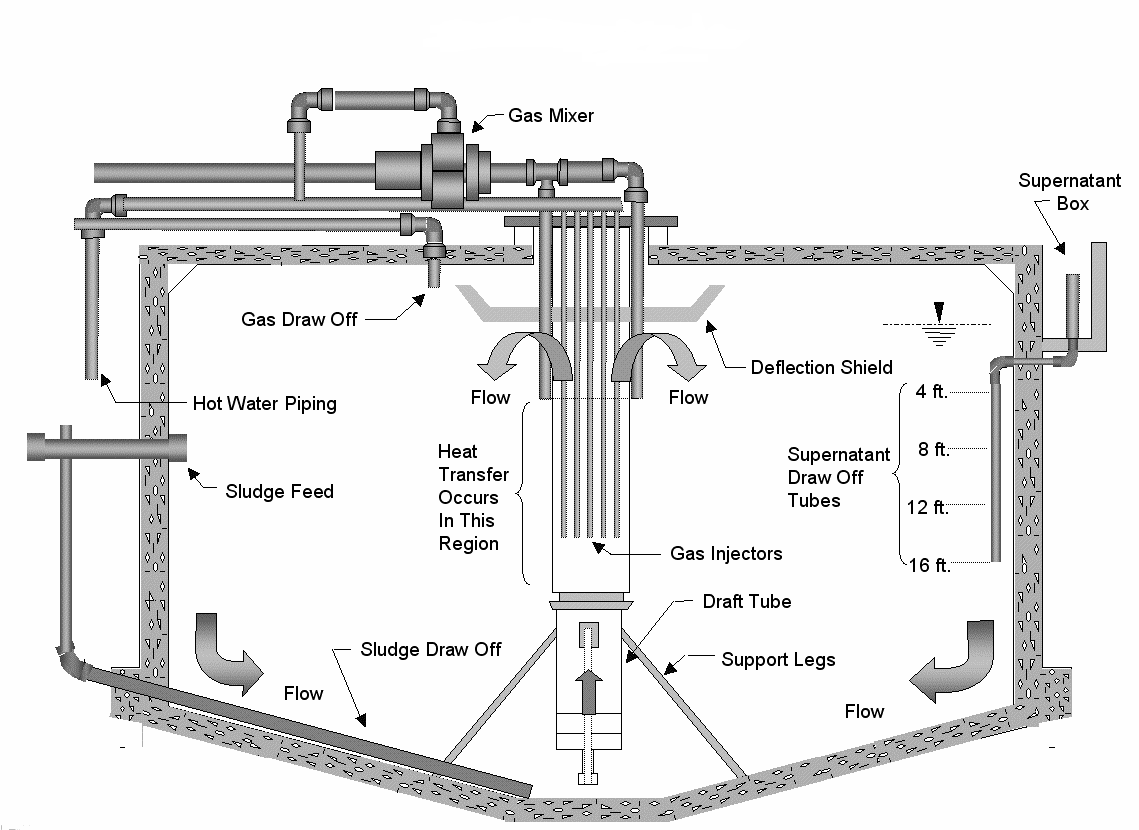
\includegraphics[scale=0.50]{DigesterFixedCover}\\
\textbf{Anaerobic Digester}\\
\end{center}
		\item The sludge typically occupies 70 - 90\% of the total digester volume and the methane carbon dioxide gas mixture occupies the headspace from where it is withdrawn also on a continuous basis.
		\item In the anaerobic digestion process microorganisms convert volatile matter into mainly methane (CH$_4$) and carbon dioxide (CO$_2$)
		\item The sludge content of the digesters is kept mixed and maintained in a constant temperature range using external heating.
		\item The activity and type of bacteria present in the digester is dictated by the operating temperature of the digester.
		\item Anaerobic digestion can be in the following three temperature ranges, each of which has its own unique microbiology.\\
			\begin{enumerate}[1. ]
			\item Psychrophilic digester:  Digester is maintained between 50  - 65 F.  Sludge detention time - 50 to 180 days
			\item Mesophilic digesters: – Digester is most commonly operated  between 95 – 98 F and the typical number of days required for digestion is between 15 to 30 days.\\
			\item Thermophilic digesters:  These digesters’ optimal operating temperatures range is between 113   135 F and it typically requires 5 to 12 days.\\
			\end{enumerate}     
		\item These organic solids are measured as volatile solids (VS).  
		\item The volatile solids content of the sludge entering and leaving the digester are measured to quantify the solids removal in the digester
		 \item Breakdown of volatile matter in the sludge ultimately into methane (CH$_4$) and carbon dioxide (CO$_2$) occurs in multiple steps involving different groups of microorganisms as follows:\\
			\begin{enumerate}[Step 1.]
			\item Hydrolysis:  Here the microorganisms breakdown complex organic matter in the sludge - carbohydrates, proteins, lignin, and lipids into simpler compounds including sugars, soluble fatty acids and amines.\\
			\item Acid Formation:  The simpler compounds formed in Step 1 are converted to organic acids by acid forming bacteria\\
			\item Methane Formation: The organic acids formed in Step 2 are converted into methane and carbon dioxide by methane forming bacteria.\\
			\end{enumerate}
		\item Gas production ranges between 10 to 16 cubic feet per pound of volatile matter destroyed and the gas production remains stable over time.
		\item Low gas production indicates problems - toxicity, temperature, volatile acid to alkalinity ratio, mixing, or feed rates.
		\end{itemize}

\newpage
\section{Chlorination}


\begin{itemize}
\item Treated wastewater effluent is disinfected prior to its discharge into a water body inorder to destroy pathogens primarily to prevent spread of waterborne disease and minimize public health problems
\item Chlorine is a very effective disinfectant and is the most widely used disinfectant for wastewater 
\item Chlorine disinfection is a practical and economical means for disinfecting large quantities of wastewaters which have been treated to various degrees. 
\item However, due to its toxicity, associated risk factors and its rising cost, use of ultraviolet light and ozone for wastewater disinfection is on the rise
\end{itemize}


\subsection{Forms of Chlorine}\index{Forms of Chlorine}

\begin{itemize}
	\item Due to safety issues related to the use of chlorine gas, 			\textbf{hypochlorites} are often used in lieu of chlorine
	\item Types of hypochlorites
	\begin{itemize}
	\item Sodium hypochlorite (NaOCl) comes in a liquid form which contains up to 12.5\% chlorine
	\item Calcium hypochlorite (Ca(OCl)$_2$), also known as HTH, is a solid which is mixed with water to form a hypochlorite solution. Calcium hypochlorite is 65-70\% concentrated.
	\end{itemize}
	\item Hypochlorites decompose in strength over time while in storage. Temperature, light, and physical energy can all break down hypochlorites before they are able to react with pathogens in water. 

\end{itemize} 

\subsection{Chlorine Properties}\index{Chlorine Properties}

\begin{itemize}
\item Chlorine is a yellowish-green gas at room temperature and atmosphric pressure
\item Chlorine gas can be pressurized and cooled to its liquid form for making it easy to ship and store. 
\item When liquid chlorine is released, it quickly turns into a gas that stays close to the ground (being heavier than air) and spreads rapidly.
	\item 	While it is not explosive or flammable, as a liquid or gas it can react violently with many substances 
	\item Chlorine is only slightly soluble in water (0.3 to 0.7\% by weight.) 
	\item Chlorine gas has a greenish-yellow color 
	\item It has a characteristic disagreeable and pungent odor, similar to chlorine-based laundry bleaches, and is detectable by smell at concentrations as low as 0.2 to 0.4 ppm
	\item It is about two and a half times as heavy as air
	\item One volume of liquid chlorine yields about 460 volumes of chlorine gas. 
	\item Liquid chlorine is amber in color and is about one and a half times as heavy as water 
	\item Chlorine is an irritant to the eyes, skin, mucous membranes, and the respiratory system 
\end{itemize}


\subsection{Chlorine Storage and Safety}\index{Chlorine Storage and Safety}


\subsubsection{Chlorine Delivery}\index{Chlorine Delivery}

\begin{itemize}
\item Typically for smaller plants chlorine gas is shipped in  pressurized steel cylinders - 150 lb or 2000 lb (ton cylinder) size
\item Larger plants may get their chlorine supply in rail tank cars
\item The daily chlorine usage is typically established based upon the weighing of the chlorine containers.
\end{itemize}


\subsubsection{Chlorine Leak Response}\index{Chlorine Leak Response}
\begin{itemize}
	\item Typically for smaller plants chlorine gas is shipped in  pressurized steel cylinders - 150 lb or 2000 lb (ton cylinder) size.  Larger plants may get their chlorine supply in rail tank cars.  
	\item The daily chlorine usage is typically established based upon the weighing of the chlorine containers.
	\item The withdrawal rates from a chlorine cylinder is based on the temperature of the liquid in the cylinder, and thus the pressure of the gas. 
	\item As chlorine gas is withdrawn from the cylinder, it absorbs the heat from the surroundings.
	\item For low withdrawal rates, heat will be able to be transferred from the surrounding air to the container in time so that there is no drop in temperature or pressure, 
	\item If the chlorine withdrawal is larger, the air will not be able to transfer the heat quickly enough and the temperature (and pressure) of the chlorine will drop, thus resulting in a lower feed rate. 
	\item If high enough and prolonged enough, this can even result in ice formation around the outside of the container, further decreasing the withdrawal rate. 
	\item The most effective way to increase withdrawal rate from a single container is to circulate the surrounding air with a fan. Again, never apply heat to the containers.
	\item If chlorine gas escapes from a container or system, being heavier than air, it will seek the lowest level in the building or area
	\item Only trained staff with access to proper personal protection equipment (PPE) including self-contained breathing apparatus, should handle the chlorine cylinders and address chlorine leak issues 
	\item When a leak is suspected, it is recommended that ammonia vapors be used to find the source. When ammonia vapor using a rag or brush, is directed at a leak, a white cloud will form. To produce ammonia vapor, a plastic squeeze bottle containing about 5 \% ammonia, aqua ammonia (ammonium hydroxide solution) should be used. A weaker solution such as household ammonia may not be concentrated enough to detect minor leaks
	\item All safety equipment should be located outside of the chlorine room and be easily accessed by all personnel
	\item Small leaks around valve stems can usually be corrected by tightening the packing nut or closing the valve. A leak can also be reduced by removing the chlorine as rapidly as possible
	\item If it cannot be added to the process there are several chemicals which can be used to absorb the chlorine gas. For example, chlorine can be absorbed by using 1$frac{1}{4}$ pounds of caustic soda or hydrated line, or 3 pounds of soda ash per pound of chlorine. 
	\item If the leaking container can be moved, it should be transported to an outdoors area where minimal harm will occur. Keep the leaking part the most elevated so that gaseous chlorine will leak rather than liquid chlorine.
	\item If the leak is large, all persons in the adjacent area must be warned and evacuated. Only authorized persons equipped with the proper breathing apparatus, and protective measures to the eyes and body should investigate. 
	\item As water is not an efficient absorbent for chlorine and the fact that chlorine reacts with water to form very corrosive hydrochloric acid, never apply water to a leak or consider submerging a chlorine cylinder (for example, in a pond or tank), since it will probably float.
	\item Remember to keep windward of the leak.
	\item As chlorine cylinders pressure increases with temperature, as a safety measure the chlorine cylinders are fitted with fusible plug which melts between 158$^o$ and 165$^o$ F.
	\item Keep chlorine cylinder or container emergency repair kits available. Be familiar with their use and location.
	\item Leaks at fusible plugs and cylinder valves requires special handling and emergency equipment. The chlorine supplier must be notified immediately
	\item Pin hole leaks in cylinder walls or ton tanks can usually be stopped by mechanical pressure applications (clamps, turnbuckles, etc.). This only temporary and may require your ingenuity.
	\item Leaking containers cannot be shipped.
	\item In general, daily inspection of all chlorine cylinders will avoid major problems
\end{itemize}

\subsubsection{Chlorine Reactions Related to Disinfection}\index{Chlorine Reactions Related to Disinfection}
\textbf{Chlorine reacts with water to form hypochlorous and hydrochloric acids}\\
Cl$_2$ \hspace{0.8cm}	+ \hspace{0.3 cm}	 H$_2$O		\hspace{0.8cm} $\iff$ 
\hspace{0.8cm} HOCl	\hspace{0.8cm}	 +	\hspace{0.8cm}	 HCl \\
chlorine \hspace{0.8cm}	water \hspace{1.8cm}		 hypochlorous acid	\hspace{0.1cm}	 hydrochloric acid\\ 
	\vspace{0.5cm}
	\begin{itemize}
		\item Hypochlorous acid dissociates in water to form the hydrogen and hypochlorite ions\\
 HOCl \hspace{1.8 cm} $\iff$ \hspace{1.8 cm} H$^+$ \hspace{1.8cm} + 	\hspace{0.8cm}OCl$^-$\\ 
hypochlorous acid  \hspace{1.9 cm}      hydrogen ion   \hspace{1.5cm}           hypochlorite ion

		\begin{itemize}
			\item Hypochlorous acid is the most effective form of chlorine available to kill microorganisms
			\item Hypochlorite ions is much less efficient disinfectant
		\end{itemize}

		\item The concentration of hypochlorous acid and hypochlorite ions in chlorinated water will depend on the water's pH
		\begin{itemize}
			\item A higher pH facilitates the formation of more hypochlorite ions and results in less hypochlorous acid in the water
		\end{itemize}
		\item A significant percentage of the chlorine is still in the form of hypochlorous acid even between pH 8 and pH 9
		\end{itemize}



\subsection{Chlorine Disinfection}\index{Chlorine Disinfection}

\begin{itemize}
\item When chlorine is added to a wastewater flow, it will first react or combine with certain organic and inorganic substances present, prior to acting on pathogens.  The amount of chlorine used up as part of these reactions is referred to as the \textbf{chlorine demand}\\

\item The \textbf{free chlorine} remaining after the chlorine demand is satisfied, is the strongest form of chlorine available for disinfection.  

\item Chlorine combined with ammonia (as chloramines) and organic compounds (as chloroorganic compounds), known as \textbf{combined chlorine} also exhibit disinfecting properties - albeit weaker than the free chlorine.

\item \text{Total residual chlorine} is the sum of free chlorine and combined chlorine and it is the residual chlorine concentration which represents the amount of chlorine available for disinfection 

\item \textbf{Chlorine Demand = Applied Chlorine Dose - Chlorine Residual}\\ Chlorine residual should be the basis of measuring the effectiveness of chlorine disinfection

\item Chlorine residuals are measured in the field using a colorimeteric method.  In the laboratory, chlorine residuals are measured typically using: 1) Amperometric Titration, or 2) Iodometric Titration

\item Chlorine dosage is typically established from either bench scale laboratory testing, or actual measurement of field results. 

\item Since field conditions, particularly the mixing element, are not as well controlled as laboratory tests, the actual dosage is expected to be generally higher than from that established in the laboratory. 

\item Even though residual chlorine concentration can be used for establishing the effectiveness of disinfection, the ultimate effectiveness of disinfection can be monitored by conducting bacteriological testing.

\end{itemize}

\subsection{Factors Affecting Chlorine Disinfection Efficiency}\index{Factors Affecting Chlorine Disinfection Efficiency}

The disinfection efficiency of chlorine depends on the following factors:\\
\begin{itemize}
	\item pH:  Disinfection is more efficient at a low pH when large quantities of hypochlorous acid are present than at a high pH when hypochlorite ions is the dominant species in the water
	\item Concentration:  Contact Time Ratio (CT):  For effective chlorine disinfection both sufficient chlorine dosages – concentration (C) as well as contact time (T) are necessary.  There may be a substantial residual but if CT factor is not adequate, disinfection may not be effective. Generally both of these factors must be worked out experimentally for a given system
	\item Temperature:  Colder temperatures are less favorable for disinfection. 
Proper contacting or mixing or agitation:  This is necessary to make sure that the chlorine applied contacts or reaches the microbial cells
	\item Organic and inorganic material present:  The chlorine used by these organic and inorganic reducing substances including metal ions, organic matter and ammonia, is defined as the chlorine demand.  So that the amount of chlorine that has to be added to wastewater for different purposes will also vary.
\item Even though residual chlorine concentration can be used for establishing the effectiveness of disinfection, the ultimate effectiveness of disinfection can be monitored by conducting bacteriological testing.
\end{itemize}
		
\subsection{Dechlorination}\index{Dechlorination}
\begin{itemize}
\item Dechlorination is the process of removing residual chlorine from disinfected wastewater prior to discharge into the environment
\item Dehlorination is necessary to mitigate the toxic effect of chlorine on the receiving waters.  
\item Sulfur dioxide is most commonly used for dechlorination.
\item Other chemicals used for sodium bisulfite, sodium sulfite and sodium thiosulfate.
\end{itemize}

\newpage

\section{Wastewater Treatment Hazards}\index{Wastewater Treatment Hazards}
There are many hazards encountered in wastewater treatment operations.  The hazards and their respective mitigation measures are as follows:\\
\subsection{Hazardous Chemicals}\index{Hazardous Chemicals}
\begin{itemize}
\item Hazardous chemicals are used throughout wastewater treatment plants and in collection systems. 
\item To understand the dangers of these chemicals and to take adequate steps OSHA requires that the chemical manufacturer, distributor, or importer provide Safety Data Sheets (SDSs) (formerly MSDSs or Material Safety Data Sheets) for each hazardous chemical to downstream users to communicate information on hazards related to that particular chemical or product.
\item Employers must ensure that the SDSs are available and readily accessible to employees for all hazardous chemicals in their workplace.
\item The SDS includes information such as the properties of each chemical; the physical, health, and environmental health hazards; protective measures; and safety precautions for handling, storing, and transporting the chemical.\\
\end{itemize}
\subsection{Hazardous Gasses}\index{Hazardous Gasses}
\begin{itemize}
\item A summary of the properties and effects of hazardous gases found in wastewater operations is provided in the table below.
\item To safeguard against the potential impacts of these gases, employees are required to follow practices including donning appropriate Personal Protective Equipment (PPE) and utilizing respiratory protection\\
\end{itemize}
\begin{center}
\includegraphics[scale=0.6]{SafetyHazardousGases4}\\ 
\end{center}

\subsection{Falls}\index{Falls}
\begin{itemize}
\item Falls are one of the leading causes of injuries and deaths on the job.  Fall protection is a combination of methods and devices used to protect workers from falling off, onto, or through working levels. 
\item Fall protection methods and devices are typically divided into two categories: those that prevent falls and those that arrest falls. 
\item Examples of fall protection methods and devices include rails, guards, guardrails, barriers, fall-arrest systems, safety nets, hole covers, and various work practices and procedures.
\end{itemize}
\begin{center}
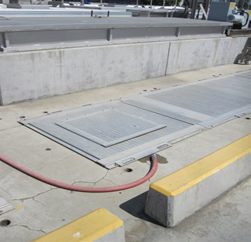
\includegraphics[scale=0.8]{SafetyFallProtection1}\hspace{1cm} 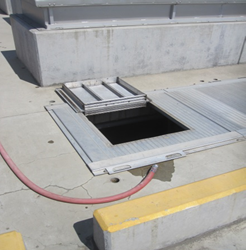
\includegraphics[scale=0.8]{SafetyFallProtection2}\\
\end{center}
\subsection{Noise}\index{Noise}
\begin{itemize}
\item Noise as a hazard is sound that is especially loud or impacting. 
\item A wastewater treatment plant has equipment that produces high noise levels both continuously and intermittently. 
\item As such, it is important to be aware of this hazard and to take preventive steps to reduce exposure to damaging noise levels by wearing effective hearing protection and to minimize the duration of the exposure to the noise.
\end{itemize}

\subsection{Electrical Hazards}\index{Electrical Hazards}
\begin{itemize}
\item Ordinary 120-V electricity can be fatal; most wastewater facility electrical systems operate at 120 to 4000 V or more.  
\item All voltages should be considered dangerous and potentially life threatening.  
\item Safe working rules and practices that should be followed when working on electrical systems
\item Before working on an electrical system, perform a job hazard analysis to determine any potential hazards and methods of abating those hazards
\end{itemize}


\subsection{Rotating and Moving Equipment}\index{Rotating and Moving Equipment}

\begin{itemize}
\item All rotating and moving equipment should be guarded. 
\item The best method for preventing machinery-related injuries is through use of equipment guards enforced through engineering and administrative controls.   
\item The best way to prevent this type of injury is to install point-of-operation guards that prevent contact with ingoing nip points, pinch points, rotating parts, flying chips, and sparks.
\end{itemize}
\begin{center}
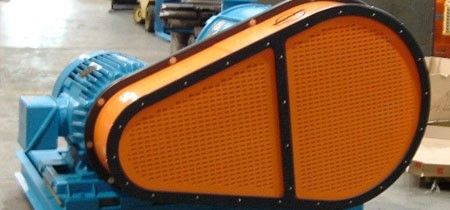
\includegraphics[scale=0.6]{SafetyMachineGuarding}\\
\end{center}

\subsection{Heat Stress}\index{Heat Stress}
\begin{itemize}
\item Heat stress falls into two categories: heat illness and heat stroke. 
\item Both are serious conditions and should not be taken lightly. 
\item Heat stress can result from: 
\begin{itemize}
\item High temperature and humidity, dehydration from low fluid consumption
\item Direct sun exposure (with no shade) or extreme heat, 
\item Limited air movement (no breeze or wind), 
\item Physical exertion, Use of bulky protective clothing and equipment, 
\item Poor physical condition or ongoing health problems, 
\item Some medications
\item Pregnancy
\end{itemize}
\end{itemize} 


\subsection{Safety Practices}\index{Safety Practices}
\subsubsection{Lockout - Tagout (LOTO)}\index{Lockout - Tagout (LOTO)}

When conducting routine inspections, repairs and maintenance activities, requires meeting the mandates of \hl{Occupational Safety  Hazard Administration(OSHAs) Lock-Out/Tag-Out (LOTO) program}\\
which is designed to prevent injury or fatalities.  It involves preventing an equipment from accidentally starting up and release of all stored energy.  Hazardous energy sources include: 
\begin{itemize}
\item Electrical 
\item Mechanical
\item Hydraulic
\item Pneumatic 
\item Chemical 
\item Thermal  
\item Other energy
\end{itemize}

The LOTO involves established and documented procedures specific to an equipment or machinery.  It typically comprises of:\\
\begin{itemize}
\item Notifying affected employees
\item Stopping and isolating the equipment
\item Releasing stored energy
\item Verification of the isolation and de-energization
\item Placing lock-out devices which use a positive means such as a lock, either key or combination type, to hold an energy isolating device in the safe position and prevent the energizing of a machine or equipment
\item Appropriately tagging the devices to indicate its non-operation and that it may not be operated until the tagout device is removed
\end{itemize}

\subsubsection{Personal Protective Equipment (PPE)}\index{Personal Protective Equipment (PPE)}
Employees depend on personal protective equipment to protect themselves from hazards and perform daily duties. PPE includes but is not limited to safety glasses, face shields, hard hats, gloves, foot protection, and durable and disposable chemical-protective clothing. Respirators and fall protection might also be required. However, respirators and fall protection fall under separate OSHA standards. \\

\subsubsection{Confined Space Entry}\index{Confined Space Entry}
OSHA defines a confined space as an area that:
\begin{itemize} 
\item is large enough and so configured that an employee's body can enter and perform assigned work
\item has limited or restricted means for entry or exit; and
\item is not designed for continuous employee occupancy.
\end{itemize}
A permit-required confined space is defined as a confined space that:
\begin{itemize} 
\item contains or has a potential to contain a hazardous atmosphere
\item contains a material that potentially could engulf an entrant
\item has an internal configuration that could trap or asphyxiate an entrant through inwardly converging walls or a floor that slopes downward and tapers to a smaller cross-section
\item contains any serious safety or health hazard
\end{itemize}

Potentially dangerous atmospheric conditions which can exist in confined spaces include: 
\begin{itemize}
\item Oxygen level: Some gasses are heavier than air and so will fill up a confined space, which forces oxygen out.  The oxygen concentration must not fall below 19.5\% at any time.  In plants where pure oxygen is used there is a potential hazard due to high the oxygen concentration.  Oxygen concentration greater than 23\% increases the risk of ignition and fire
\item Explosive conditions:  Many gasses are explosive when present in certain ratios with oxygen. These ratios are defined by the upper explosive limit(UEL) and the lower explosive limit (LEL).  The minimum concentration of a particular combustible gas or vapor necessary to support its combustion in air is defined as the Lower Explosive Limit (LEL) for that gas. Below this level, the mixture is too “lean” to burn. The maximum concentration of a gas
or vapor that will burn in air is defined as the Upper Explosive Limit (UEL). Above this level, the mixture is too “rich” to burn.  The range between the LEL and UEL is known as the flammable range for that gas or vapor.  
\item Toxic conditions:  This condition could potentially exist due to the presence of gasses such as carbon dioxide, chlorine and hydrogen sulfide.  
\end{itemize}
\chapterimage{MathCover.png} % Chapter heading image

\chapter{Math Problems - Part II}

\section{Trickling Filters}\index{Trickling Filters}

\subsection{Example Problems} \index{Example Problems}

\begin{enumerate}


\item The total influent flow (including recirculation) to a trickling filter is 1.89 MGD. If the trickling filter is 80 ft in diameter, what is the hydraulic loading in gpd/sq ft on the trickling filter?\\
Solution:\\
$Hydraulic \enspace loading \enspace \dfrac{gpd}{ft^2}=\dfrac{(1.89*10^6)gpd}{(0.785*80^2)ft^2} =\boxed{376\dfrac{gpd}{ft^2}}$

\item A trickling filter, 70 ft in diameter with a media depth of 6 ft, receives a flow of 0.78 MGD. If the BOD concentration of the primary effluent is 167 mg/L, what is the organic loading on the trickling filter in lbs BOD/day/1000 cu ft?\\
Solution:  $Organic \enspace loading:\dfrac{lbs \enspace BOD}{day-1000ft^3}=\dfrac{lbs \enspace BOD \enspace feed \enspace to \enspace TF \enspace per \enspace day}{volume \enspace in \enspace 1000ft^3}$\\
$=\dfrac{\dfrac{(0.78*167*8.34)lbs \enspace BOD}{day}}{(0.785*70^2*6)ft^3*\dfrac{1000ft^3}{1000ft^3}}=\boxed{\dfrac{47 lbs \enspace BOD}{day-1000 ft^3}}$

\item The suspended solids concentration entering a trickling filter is 236 mg/l. If the suspended solids concentration of the trickling filter effluent is 33 mg/l, what is the suspended solids removal efficiency of the trickling filter?\\
Solution:\\
$\% Removal=\dfrac{236 mg/l-33 mg/l}{236 mg/l}*100=\boxed{86\%}$


\item A trickling filter, 70 ft in diameter with a media depth of 6 ft, receives a flow of 0.78 MGD. If the BOD concentration of the primary effluent is 167 mg/L, what is the organic loading on the trickling filter in lbs BOD/day/1000 cu ft?\\
Solution:\\
$Organic \enspace loading:\dfrac{lbs \enspace BOD}{day-1000ft^3}=\dfrac{lbs \enspace BOD \enspace feed \enspace to \enspace TF \enspace per \enspace day}{volume \enspace in \enspace 1000ft^3}$\\
$=\dfrac{\dfrac{(0.78*167*8.34)lbs \enspace BOD}{day}}{(0.785*70^2*6)ft^3*\dfrac{1000ft^3}{1000ft^3}}=\boxed{\dfrac{47 lbs \enspace BOD}{day-1000 ft^3}}$

\item The influent to the trickling filter is 1.61 MGD. If the recirculated flow is 2.27 MGD, what is the recirculation ratio?\\
Solution:  $R_R=\dfrac{Q_R}{Q_I}=\dfrac{2.27}{1.61}=\boxed{1.4}$\\
\end{enumerate}

\subsection{Practice Problems} \index{Practice Problems}

\begin{enumerate}

\item A trickling filter has a total flow of 32 MGD.  If the recirculation ratio is 0.8, what is the primary effluent flow to the TF?\\


\item A 80-ft diameter trickling filter with a media depth of 7 ft receives a primary influent flow of 2,180,000 MGD. If the BOD concentration of the primary effluent is 139 mg/L, what is the organic loading on the trickling filter in lbs BOD/day/1000 cu ft? (Ans: 72 lbs/day-1000 ft3)\\

\item The desired trickling filter recirculation ratio is 1.4.  If the primary effluent flow is 4.4 MGD what is the trickling filter effluent flow that needs to be recirculated.\\

\item A 90 ft diameter trickling filter treats a 540,000 gpd primary effluent flow. If the recirculated flow to the trickling filter is 120,000 gpd, what is the hydraulic loading on the trickling filter in gpd/ft2.\\

\end{enumerate}


\newpage

\section{Stabilization Ponds}\index{Stabilization Ponds}

\subsection{Example Problems} \index{Example Problems}

\begin{enumerate}

\item What is the surface area in acres of a pond that is 4 feet deep, if it holds 30 million gallons?\\

Solution:\\
$Pond \enspace Volume= Surface \enspace Area*Depth \implies 30MG=Surface \enspace Area*4ft$\\
$ \implies Surface \enspace Area \enspace (acres)=\dfrac{30MG*3.069\dfrac{acre-ft}{MG}}{4ft}=\boxed{23 \enspace acre}$


\item The influent flow to a pond is 10,000 gallons/hour with a suspended solids concentration of 142mg/L in the raw wastewater.  How many lbs of suspended solids are sent to the pond daily?
\\
Solution:\\
$\dfrac{lbs SS}{day}=10000\dfrac{gal}{hr}*\dfrac{24hrs}{day}*\dfrac{MG}{1000000gal}*142\dfrac{mg}{l}*8.34=\boxed{284\dfrac{lbs \enspace SS}{day}}$


\item A pond is 260 ft. long and 80 ft. wide. What is the area of this pond in acres?\\ 
Solution:\\
$(260*80)ft^2*\dfrac{acre}{43,560ft^2}=\boxed{0.48acre}$

\item A pond has a volume of 1,800,000 $ft^3$. If the flow to the pond is 425 gpm, what is the pond detention time in days?
\\
Solution:\\
$DT=\dfrac{volume}{flow}=1,800,000ft^3*\dfrac{1}{425\dfrac{gal}{min}}*\dfrac{day}{1440min}*\dfrac{7.48gal}{ft^3}=\boxed{22days}$

\item Find pond hydraulic loading in inches/day when the depth of the pond is 6 ft. and the detention time is 30 days.\\
Solution:\\

$Hydraulic \enspace Loading \enspace (HL)=\dfrac{flow}{area}$\\
$Detention \enspace time \enspace (DT)=\dfrac{vol}{flow} \implies flow=\dfrac{vol}{DT} $\\
Substituting \enspace for \enspace flow \enspace in \enspace the HL \enspace formula above:\\
$HL=\dfrac{\dfrac{vol}{DT}}{area}\enspace or \enspace \dfrac{vol}{area*DT} \enspace \implies \boxed{HL=\dfrac{pond \enspace depth}{DT}} \enspace as \enspace \dfrac{vol}{area}=pond \enspace depth$\\

$Pond \enspace hydraulic \enspace loading \enspace rate=\dfrac{Pond \enspace depth \enspace (in)}{Pond \enspace detention  \enspace time \enspace \dfrac{Volume}{Flow}}=\dfrac{6*12 \enspace inches}{30 \enspace days}=\boxed{\dfrac{2.4in}{day}}$\\
\vspace{0.5cm}

\item The flow to a pond is 750,000 gpd. If the pond diameter is 100 ft and the BOD in the pond influent is 300 mg/L, what is the organic loading to this pond in lbs BOD/day/acre?
\\
Solution:\\
$Organic \enspace loading=\dfrac{lbs \enspace BOD \enspace per \enspace day}{area \enspace (acres)}=\dfrac{0.75MGD \enspace * \enspace 300mg/l \enspace * \enspace 8.34}{0.785*100^2ft^2}*\dfrac{43,560ft^2}{acre}=\boxed{\dfrac{10,413lbs \enspace BOD}{day-acre}}$
\end{enumerate}

\subsection{Practice Problems} \index{Practice Problems}

\begin{enumerate}

\item A stabilization pond is 1100 ft. long, 600 ft wide, and is operated at a depth of 5 ft. It receives a flow of 500,000 gpd and which has an influent BOD of 185mg/L.  Using this information do the following:
\begin{enumerate}
\item Convert the flow to the pond in units of acre-ft/day.
\item Find the area of this pond in units of acres.
\item Find the volume of pond in units of acre-feet.
\item Calculate the pond detention time in days.
\item Calculate the hydraulic loading to the pond in units of inches per day.
\item Calculate the organic loading to the pond (lbs of BOD/day/acre).
\end{enumerate}

\item  A 2.5 acre stabilization pond is operated at a depth of five (5) ft. What is the pond detention time if the flow to the pond is 18,000 $ft^3$/day? 

\item The flow to a pond is 7.2MGD. If the pond diameter is 350 ft and the BOD in the pond influent is 170mg/L, what is the organic loading to this pond in lbs BOD/day/acre?
\\
\end{enumerate}


\newpage

\section{Activated Sludge}\index{Activated Sludge}

\subsection{Example Problems} \index{Example Problems}

\begin{enumerate}
\item Calculate F/M ratio based on the following data:\\
Secondary influent BOD - 156 mg/l\\
Four (4) aeration basins - 30 ft x 70 ft x 10 ft. deep\\
Influent flow - 0.65 MGD\\
MLSS - 3600 mg/l\\
MLSS average \% volatile - 72\%\\
Solution:\\
\vspace{0.3cm}
$F:M=\dfrac{(lbs/day) \enspace primary \enspace effluent  \enspace BOD \enspace entering \enspace the  \enspace aeration \enspace tank}{(lbs) \enspace MLVSS \enspace in \enspace the  \enspace aeration \enspace tank}$\\
\vspace{0.3cm}
$F:M=\dfrac{156*0.65*8.34}{3600*0.72*4*(30*70*10)ft^3* \dfrac{7.48gal}{ft^3}*\dfrac{MG}{1000000gal}*8.34}=\boxed{0.06}$\\

\item Calculate the MCRT of an activated sludge plant given the following information.\\
Plant flow- 4.25 MGD\\
WAS conc-7980 mg/l\\
Waste flow- 0.055 MGD\\
RAS conc.- 7980 mg/l\\
Aeration tank vol-1MG\\  
Clarifier vol- 0.25 MG\\
Final eff TSS conc. - 21.2 mg/l\\
MLSS conc.- 2050 mg/l\\
\vspace{0.3cm}
Solution:\\
\vspace{0.3cm}
$MCRT (days) =  \dfrac{MLSS \enspace in \enspace aeration \enspace tank \enspace (lbs)+MLSS \enspace in \enspace clarifier \enspace (lbs)}{SS \enspace effluent \enspace (lbs/day)+SS \enspace WAS \enspace (lbs/day)}$\\
\vspace{0.3cm} 
$MLSS \enspace in \enspace aeration \enspace tank \enspace (lbs)=1*2050*8.34=17097lbs$\\
\vspace{0.3cm} 
$MLSS \enspace in \enspace clarifier \enspace (lbs)=0.25*2050*8.34=4274.3lbs$\\
\vspace{0.3cm} 
$SS \enspace effluent \enspace (lbs/day)=4.25MGD *21.2mg/l*8.34=751.4lbs/day$\\
\vspace{0.3cm} 
$SS \enspace WAS \enspace (lbs/day)=0.055MGD *7980mg/l*8.34=3660.4lbs/day$\\
\vspace{0.3cm} 
Plugging in the values calculated above: $MCRT (days) =  \dfrac{17097.6+4274.3}{751.4+3660.4}=4.8=\boxed{5days}$\\
\vspace{0.2cm}


\item A sludge settleability test shows a reading 220 ml after 30 minutes of settling in a one liter graduated cylinder. Lab testing on this mixed liquor shows a MLSS concentration of 1850 mg/L and a MLVSS concentration of 1440 mg/L. Calculate SVI for this mixed liquor sample.\\

Solution:\\
SVI (ml/g)= $\dfrac{Settled \enspace sludge \enspace volume \enspace in \enspace ml/l \enspace after \enspace 30 \enspace min}{MLSS \enspace mg/l}*1000 \dfrac{mg}{g}$\\
\vspace{0.5cm}
SVI=$\dfrac{220ml/l}{1,850mg/l}*1000\dfrac{mg}{g}=\boxed{119ml/g}$


\end{enumerate}

\subsection{Practice Problems} \index{Practice Problems}

\begin{enumerate}

\item What is the food/microorganism ratio given the following conditions:\\
MLSS = 2500 mg/L\\
Secondary Influent BOD$_5$ = 210 mg/L\\
Aeration Tank Volume = 125,000 gallons\\
Primary Effluent BOD$_5$ = 102 mg/L\\
Influent Flow = 235,000 gallons per day\\
Mixed Liquor is 75\% volatile\\

\item Calculate the MCRT given the following.\\
Plant flow - 1.8 MGD\\
MLSS conc -  2800 mg/l\\
WAS flow - 0.04 MGD\\
MLVSS conc. - 2190 mg/l\\
Aerator vol - 0.3 MG\\
Reactor vol. - 0.2 MG\\
RAS conc. - 8150 mg/l\\
Effluent SS conc.-18 mg/l\\

\item In an aeration tank, the MLSS is 2650 mg/l and recorded 30-minute settling test indicates 221 ml/L.  What is the sludge volume index?\\

\item The desired F/M ratio is .35 lbs BOD/day/lb MLVSS. If 2,100 lbs of BOD enter the aerator daily, how many lbs of MLVSS should be maintained in the aeration tank?\\


\end{enumerate}






\newpage

\section{Digestion}\index{Digestion}

\subsection{Example Problems} \index{Example Problems}

\begin{enumerate}

\item Calculate the volatile solids reduction in an anaerobic digester given the following information: Raw sludge feed to digester: 73.7 \% VS and digested sludge: 57.2 \%VS\\

Solution:\\
\vspace{0.5cm}
$Digester \enspace VS \enspace reduction (\%)=\dfrac{VS_{in}-VS_{out}}{VS_{in}-VS_{in}*VS_{out}}*100$\\
\vspace{0.5cm}
$Digester \enspace VS \enspace reduction (\%)=\dfrac{0.737-0.572}{0.737-0.737*0.572}*100=\boxed{ 52.3\%}$\\

\item 10,000 gallons/day of sludge is pumped to an anaerobic digester/day at 4\% solids (70\% VS).  If 50\% of the VS is destroyed, how many lbs of VS is destroyed per day?\\
Solution:\\
$\dfrac{10,000 \enspace Gal}{day}*\dfrac{8.34 \enspace lbs \enspace sludge}{Gal} \dfrac{0.04*0.7 \enspace lbs \enspace VS \enspace feed}{lb \enspace sludge}*\dfrac{0.5 \enspace lbs \enspace VS \enspace destroyed}{lbs \enspace VS \enspace feed}=\boxed{\dfrac{1,168 \enspace lbs \enspace VS \enspace destroyed}{day} } $

\item How many pounds of solids are pumped to a digester each day if the digester receives 10,000 gpd of sludge at 5\% solids concentration?\\

Solution:\\

{
$
	\dfrac{lbs \enspace TS}{day}
	=
	\dfrac{10,000 gal \enspace sludge}{day}
	*
	\dfrac{(8.34*0.05 lbs TS )}{gal \enspace sludge}
	=4,170
	\dfrac{lbs \enspace TS}{day}
$
}\\

\item Calculate the VS loading to the digester in lbs/day if 10,000 gallons of sludge containing 5\% TS with and average VS content of 78\%\\
Solution:\\
Digester VS loading (lbs/day)\\$=\dfrac{10,000 \enspace gallons \enspace sludge}{day}*\dfrac{8.34lbs \enspace sludge}{gal}*\dfrac{0.05*0.78lbs VS}{lb \enspace sludge}=\boxed{3,253lbs \enspace sludge \enspace per \enspace day}$




\end{enumerate}

\subsection{Practice Problems} \index{Practice Problems}

\begin{enumerate}

\item 10,000 gallons/day of sludge is pumped to an anaerobic digester/day at 4\% solids (70\% VS).  If 50\% of the VS is destroyed, how many lbs of VS is destroyed per day?\\

\item Primary sludge containing five percent (5\%) solids is pumped to a digester continuously at a rate of 25 gpm. How many pounds of volatile solids are added to the digester each day if the volatile solids content is 73\% of the total solids?\\

\item Calculate the \% VS reduction in a digester given the volatile solids content of the influent sludge to the digester is 70\% and the volatile solids content of the sludge leaving the digester is 52.5\%\\

\end{enumerate}

\newpage
\section{Chlorine Disinfection}\index{Chlorine Disinfection}

\subsection{Example Problems} \index{Example Problems}

\begin{enumerate}

\item Calculate how many pounds per day of chlorine should be used to maintain a dosage of 12 mg/l at a 5.0 MGD flow.\\
Solution:\\
$lbs/day=conc. (mg/l)*flow(MGD)*8.34$\\
$lbs/day=12*5*8.34=\boxed{500.4lbs/day}$\\
\item What is the chlorine demand if the chlorine dosage is 15 mg/L and the residual is 3 mg/l?
Solution:\\
Chlorine dosage = chlorine demand + chlorine residual\\
$\implies chlorine \enspace demand = chlorine \enspace dosage - chlorine \enspace residual=15-3=\boxed{12mg/l}$
\item If 80 pounds of chlorine are applied each day to a flow of 1.5 MGD, what is the dosage in mg/l?\\
Solution:\\
Applying the pounds formula:\\  $lbs/day=conc. (mg/l)*flow(MGD)*8.34$\\
$\implies conc. (mg/l)=\dfrac{lbs/day}{flow(MGD)*8.34}=\dfrac{80}{1.5*8.34}=\boxed{6.4mg/l}$
\item How many pounds per day of chlorine will be required to disinfect a secondary effluent flow of 1.68 MGD if the chlorine demand is found to be 8.5 mg/l and a residual of 3 mg/l is desired?
Chlorine dosage = chlorine demand + chlorine residual\\
$chlorine \enspace dosage=8.5+3=11.5mg/l$\\
$lbs/day=conc. (mg/l)*flow(MGD)*8.34=1.68*11.5*8.34=\boxed{161.2lbs/day}$\\


\end{enumerate}

\subsection{Practice Problems} \index{Practice Problems}

\begin{enumerate}


\item The chlorine demand is 4.8 mg/l and a chlorine residual is 0.75 mg/l is desired. For a flow of 2.8 MGD, how many pounds per day should the chlorinator be set to deliver.\\

\item Chlorine is being fed at the rate of 75 pounds per day. Plant flow is 1.2 MGD. The chlorine residual is measured and found to be 2.6 mg/L Calculate chlorine demand.\\


\end{enumerate}


\chapterimage{Dewatering.jpg} % Chapter heading image

\chapter{Part II - Practice Math Problems Solutions}

\section{Trickling Filters}\index{Trickling Filters}
\begin{enumerate}

\item A trickling filter has a total flow of 32 MGD.  If the recirculation ratio is 0.8, what is the primary effluent flow to the TF?\\
Solution:\\
$Total \enspace Flow (Q_T) = Influent \enspace Flow (Q_I)*(Recirculation \enspace Ratio(R_R) +1)$\\
$\implies 32 MGD=Q_I*(0.8+1)\implies Q_I=\dfrac{32}{1.8}=\boxed{17.8 MGD}$

\item A 80-ft diameter trickling filter with a media depth of 7 ft receives a primary influent flow of 2,180,000 MGD. If the BOD concentration of the primary effluent is 139 mg/L, what is the organic loading on the trickling filter in lbs BOD/day/1000 cu ft? (Ans: 72 lbs/day-1000 ft3)\\
Solution:\\
$Organic \enspace loading:\dfrac{lbs \enspace BOD}{day-1000ft^3}=\dfrac{lbs \enspace BOD \enspace feed \enspace to \enspace TF \enspace per \enspace day}{volume \enspace in \enspace 1000ft^3}$\\
\vspace{0.3cm}
$\implies Organic \enspace loading=\dfrac{\dfrac{(2.18*139*8.34)lbs \enspace BOD}{day}}{(0.785*80^2*7)ft^3*\dfrac{1000ft^3}{1000ft^3}}=\boxed{\dfrac{72 lbs \enspace BOD}{day-1000 ft^3}}$

\item The desired trickling filter recirculation ratio is 1.4.  If the primary effluent flow is 4.4 MGD what is the trickling filter effluent flow that needs to be recirculated.\\
Solution:\\
$R_R=\dfrac{Q_R}{Q_I}\implies 1.4=\dfrac{Q_R}{4.4}\implies Q_R =1.4*4.4=\boxed{6.2 MGD}$\\

\item A 90 ft diameter trickling filter treats a 540,000 gpd primary effluent flow. If the recirculated flow to the trickling filter is 120,000 gpd, what is the hydraulic loading on the trickling filter in gpd/ft2.\\
Solution:\\
$Hydraulic \enspace loading:\dfrac{gpd}{ft^2} \implies Hydraulic \enspace loading \enspace \dfrac{gpd}{ft^2}=\dfrac{(540,000+120,000)gpd}{(0.785*90^2)ft^2} =\boxed{104\dfrac{gpd}{ft^2}}$

\end{enumerate}

\section{Stabilization Ponds}\index{Stabilization Ponds}
\begin{enumerate}

\item A stabilization pond is 1100 ft. long, 600 ft wide, and is operated at a depth of 5 ft. It receives a flow of 500,000 gpd and which has an influent BOD of 185mg/L.  Using this information do the following:
\begin{enumerate}
\item Convert the flow to the pond in units of acre-ft/day.
\item Find the area of this pond in units of acres.
\item Find the volume of pond in units of acre-feet.
\item Calculate the pond detention time in days.
\item Calculate the hydraulic loading to the pond in units of inches per day.
\item Calculate the organic loading to the pond (lbs of BOD/day/acre).
\end{enumerate}


Solution:\\
\begin{enumerate}
\item $\dfrac{500,000gal}{day}*\dfrac{ft^3}{7.48gal}*\dfrac{acre-ft}{43,560ft^3}=\boxed{1.53\dfrac{acre-ft}{day}}$
\item $(1,100*600)ft^2*\dfrac{acres}{43,560 ft^2}=\boxed{15.2acres}$
\item $(1,100*600*5)ft^3*\dfrac{acres-ft}{43,560 ft^3}=\boxed{75.8 acre-ft}$
\item $DT=\dfrac{volume}{flow}=(1,100*600*5)ft^3*\dfrac{1}{500,000\dfrac{gal}{day}}\dfrac{7.48gal}{ft^3}=\boxed{49.4days}$
\item $Pond \enspace hydraulic \enspace loading \enspace rate \Bigg[\dfrac{in}{day}\Bigg]=\dfrac{Pond \enspace depth \enspace (in)}{Pond \enspace detention  \enspace time \enspace \dfrac{Volume}{Flow}}=\dfrac{5*12in}{49.4}=\boxed{1.2\dfrac{in}{day}}$ \\
\item $Organic \enspace loading=\dfrac{lbs \enspace BOD \enspace per \enspace day}{area \enspace (acres)}$\\
$\implies \dfrac{0.5MGD \enspace * \enspace 185mg/l \enspace * \enspace 8.34}{1,100*600ft^2}*\dfrac{43,560ft^2}{acre}=\boxed{\dfrac{50.9lbs \enspace BOD}{day-acre}}$
\end{enumerate}

\item  A 2.5 acre stabilization pond is operated at a depth of five (5) ft. What is the pond detention time if the flow to the pond is 18,000 $ft^3$/day? 

Solution:\\
$Pond \enspace detention \enspace time=\dfrac{Volume}{Flow}=\dfrac{(2.5*5)acre-ft}{18,000\dfrac{ft^3}{day}*\dfrac{acre-ft}{43,560ft^3}}=\boxed{30 \enspace days}$\\ 

\item The flow to a pond is 7.2MGD. If the pond diameter is 350 ft and the BOD in the pond influent is 170mg/L, what is the organic loading to this pond in lbs BOD/day/acre?
\\
Solution:\\
$Organic \enspace loading=\dfrac{lbs \enspace BOD \enspace per \enspace day}{area \enspace (acres)}=\dfrac{7.2MGD \enspace * \enspace 170mg/l \enspace * \enspace 8.34}{0.785*350^2ft^2}*\dfrac{43,560ft^2}{acre}=\boxed{\dfrac{4,624lbs \enspace BOD}{day-acre}}$
\end{enumerate}
\section{Activated Sludge}\index{Activated Sludge}
\begin{enumerate}

\item What is the food/microorganism ratio given the following conditions:\\
MLSS = 2500 mg/L\\
Secondary Influent BOD$_5$ = 210 mg/L\\
Aeration Tank Volume = 125,000 gallons\\
Primary Effluent BOD$_5$ = 102 mg/L\\
Influent Flow = 235,000 gallons per day\\
Mixed Liquor is 75\% volatile\\

Solution:\\
\vspace{0.3cm}
$F:M=\dfrac{(lbs/day) \enspace primary \enspace effluent  \enspace BOD \enspace entering \enspace the  \enspace aeration \enspace tank}{(lbs) \enspace MLVSS \enspace in \enspace the  \enspace aeration \enspace tank}$\\
\vspace{0.3cm}
$F:M=\dfrac{210 \enspace mg/l*0.235 \enspace MGD*8.34}{\big(2500 \enspace mg/l*0.75\big)*\bigg(125,000 \enspace gal*\dfrac{MG}{1,000,000 \enspace gal}\bigg)*8.34}=\boxed{0.21}$\\

\item Calculate the MCRT given the following.\\
Plant flow - 1.8 MGD\\
MLSS conc -  2800 mg/l\\
WAS flow - 0.04 MGD\\
MLVSS conc. - 2190 mg/l\\
Aerator vol - 0.3 MG\\
Reactor vol. - 0.2 MG\\
RAS conc. - 8150 mg/l\\
Effluent SS conc.-18 mg/l\\
Solution:\\
\vspace{0.2cm}
$MCRT (days) =  \dfrac{MLSS \enspace in \enspace aeration \enspace tank \enspace (lbs)+MLSS \enspace in \enspace clarifier \enspace (lbs)}{SS \enspace effluent \enspace (lbs/day)+SS \enspace WAS \enspace (lbs/day)}$\\
\vspace{0.3cm} 
$MLSS \enspace in \enspace aeration \enspace tank \enspace (lbs)=0.3*2800*8.34=7005.6lbs$\\
\vspace{0.3cm} 
$MLSS \enspace in \enspace clarifier \enspace (lbs)=0.2*2800*8.34=4670.4lbs$\\
\vspace{0.3cm} 
$SS \enspace effluent \enspace (lbs/day)=1.8MGD *18mg/l*8.34=270.2lbs/day$\\
\vspace{0.3cm} 
$SS \enspace WAS \enspace (lbs/day)=0.04MGD *8150mg/l*8.34=2718.8lbs/day$\\
\vspace{0.3cm} 
Plugging in the values calculated above: $MCRT (days) =  \dfrac{7005.6+4670.4}{270.2+2718.8}=3.9=\boxed{4days}$\\
\vspace{0.2cm}

\item In an aeration tank, the MLSS is 2650 mg/l and recorded 30-minute settling test indicates 221 ml/L.  What is the sludge volume index?\\
\vspace{0.3cm}
Solution:\\
SVI (ml/g)= $\dfrac{Settled \enspace sludge \enspace volume \enspace in \enspace ml/l \enspace after \enspace 30 \enspace min}{MLSS \enspace mg/l}*1000 \dfrac{mg}{g}$\\
\vspace{0.5cm}
SVI=$\dfrac{221ml/l}{2650mg/l}*1000\dfrac{mg}{g}=\boxed{83ml/g}$
\item The desired F/M ratio is .35 lbs BOD/day/lb MLVSS. If 2,100 lbs of BOD enter the aerator daily, how many lbs of MLVSS should be maintained in the aeration tank?\\
Solution:\\
$F:M=\dfrac{(lbs/day) \enspace primary \enspace effluent  \enspace BOD \enspace entering \enspace the  \enspace aeration \enspace tank}{(lbs) \enspace MLVSS \enspace in \enspace the  \enspace aeration \enspace tank}$\\
\vspace{0.3cm}
$\implies 0.35=\dfrac{2100}{x}\implies x = \boxed{6000lbs \enspace MLVSS}$\\

\end{enumerate}

\section{Digestion}\index{Digestion}
\begin{enumerate}

\item 10,000 gallons/day of sludge is pumped to an anaerobic digester/day at 4\% solids (70\% VS).  If 50\% of the VS is destroyed, how many lbs of VS is destroyed per day?\\
Solution:\\
$\dfrac{10,000 \enspace Gal}{day}*\dfrac{8.34 \enspace lbs \enspace sludge}{Gal} \dfrac{0.04*0.7 \enspace lbs \enspace VS \enspace feed}{lb \enspace sludge}*\dfrac{0.5 \enspace lbs \enspace VS \enspace destroyed}{lbs \enspace VS \enspace feed}=\boxed{\dfrac{1,168lbs \enspace VS \enspace destroyed}{day} } $


\item Primary sludge containing five percent (5\%) solids is pumped to a digester continuously at a rate of 25 gpm. How many pounds of volatile solids are added to the digester each day if the volatile solids content is 73\% of the total solids?\\
Solution:\\
Digester VS loading (lbs/day)\\$=\dfrac{25*1,440 \enspace gallons \enspace sludge}{day}*\dfrac{8.34lbs \enspace sludge}{gal}*\dfrac{0.05*0.73lbs VS}{lb \enspace sludge}=\boxed{10,960 \enspace lbs \enspace sludge \enspace per \enspace day}$\\


\item Calculate the \% VS reduction in a digester given the volatile solids content of the influent sludge to the digester is 70\% and the volatile solids content of the sludge leaving the digester is 52.5\%\\
Solution:  $Digester \enspace VS \enspace reduction (\%)=\dfrac{0.7-0.525}{0.7-0.7*0.525}*100=\boxed{ 53\%}$\\

\end{enumerate}
\section{Chlorine Disinfection}\index{Chlorine Disinfection}
\begin{enumerate}
\item The chlorine demand is 4.8 mg/l and a chlorine residual is 0.75 mg/l is desired. For a flow of 2.8 MGD, how many pounds per day should the chlorinator be set to deliver.\\
Solution:\\
Chlorine dosage = chlorine demand + chlorine residual\\
$chlorine \enspace dosage=4.8+0.75=5.55mg/l$\\
To calculate pounds per day, applying the pounds formula:\\  
$lbs/day=conc. (mg/l)*flow(MGD)*8.34=2.8*5.55*8.34=\boxed{129.6lbs/day}$\\

\item Chlorine is being fed at the rate of 75 pounds per day. Plant flow is 1.2 MGD. The chlorine residual is measured and found to be 2.6 mg/L Calculate chlorine demand.\\
Solution:\\
$Chlorine \enspace dosage (lbs/day)=conc. (mg/l)*flow(MGD)*8.34$\\
$\implies chlorine \enspace dosage \enspace conc. (mg/l)=\dfrac{lbs/day}{flow(MGD)*8.34}=\dfrac{75}{1.2*8.34}=7.5mg/l$\\
Chlorine dosage = chlorine demand + chlorine residual\\
$ \implies chlorine \enspace demand = chlorine \enspace dosage - chlorine \enspace residual=7.5-2.6=\boxed{4.9mg/l}$

\end{enumerate}


%\chapterimage{MathCover.png} % Chapter heading image

\chapter{Math Problems - Part II}

\section{Trickling Filters}\index{Trickling Filters}

\subsection{Example Problems} \index{Example Problems}

\begin{enumerate}


\item The total influent flow (including recirculation) to a trickling filter is 1.89 MGD. If the trickling filter is 80 ft in diameter, what is the hydraulic loading in gpd/sq ft on the trickling filter?\\
Solution:\\
$Hydraulic \enspace loading \enspace \dfrac{gpd}{ft^2}=\dfrac{(1.89*10^6)gpd}{(0.785*80^2)ft^2} =\boxed{376\dfrac{gpd}{ft^2}}$

\item A trickling filter, 70 ft in diameter with a media depth of 6 ft, receives a flow of 0.78 MGD. If the BOD concentration of the primary effluent is 167 mg/L, what is the organic loading on the trickling filter in lbs BOD/day/1000 cu ft?\\
Solution:  $Organic \enspace loading:\dfrac{lbs \enspace BOD}{day-1000ft^3}=\dfrac{lbs \enspace BOD \enspace feed \enspace to \enspace TF \enspace per \enspace day}{volume \enspace in \enspace 1000ft^3}$\\
$=\dfrac{\dfrac{(0.78*167*8.34)lbs \enspace BOD}{day}}{(0.785*70^2*6)ft^3*\dfrac{1000ft^3}{1000ft^3}}=\boxed{\dfrac{47 lbs \enspace BOD}{day-1000 ft^3}}$

\item The suspended solids concentration entering a trickling filter is 236 mg/l. If the suspended solids concentration of the trickling filter effluent is 33 mg/l, what is the suspended solids removal efficiency of the trickling filter?\\
Solution:\\
$\% Removal=\dfrac{236 mg/l-33 mg/l}{236 mg/l}*100=\boxed{86\%}$


\item A trickling filter, 70 ft in diameter with a media depth of 6 ft, receives a flow of 0.78 MGD. If the BOD concentration of the primary effluent is 167 mg/L, what is the organic loading on the trickling filter in lbs BOD/day/1000 cu ft?\\
Solution:\\
$Organic \enspace loading:\dfrac{lbs \enspace BOD}{day-1000ft^3}=\dfrac{lbs \enspace BOD \enspace feed \enspace to \enspace TF \enspace per \enspace day}{volume \enspace in \enspace 1000ft^3}$\\
$=\dfrac{\dfrac{(0.78*167*8.34)lbs \enspace BOD}{day}}{(0.785*70^2*6)ft^3*\dfrac{1000ft^3}{1000ft^3}}=\boxed{\dfrac{47 lbs \enspace BOD}{day-1000 ft^3}}$

\item The influent to the trickling filter is 1.61 MGD. If the recirculated flow is 2.27 MGD, what is the recirculation ratio?\\
Solution:  $R_R=\dfrac{Q_R}{Q_I}=\dfrac{2.27}{1.61}=\boxed{1.4}$\\
\end{enumerate}

\subsection{Practice Problems} \index{Practice Problems}

\begin{enumerate}

\item A trickling filter has a total flow of 32 MGD.  If the recirculation ratio is 0.8, what is the primary effluent flow to the TF?\\


\item A 80-ft diameter trickling filter with a media depth of 7 ft receives a primary influent flow of 2,180,000 MGD. If the BOD concentration of the primary effluent is 139 mg/L, what is the organic loading on the trickling filter in lbs BOD/day/1000 cu ft? (Ans: 72 lbs/day-1000 ft3)\\

\item The desired trickling filter recirculation ratio is 1.4.  If the primary effluent flow is 4.4 MGD what is the trickling filter effluent flow that needs to be recirculated.\\

\item A 90 ft diameter trickling filter treats a 540,000 gpd primary effluent flow. If the recirculated flow to the trickling filter is 120,000 gpd, what is the hydraulic loading on the trickling filter in gpd/ft2.\\

\end{enumerate}


\newpage

\section{Stabilization Ponds}\index{Stabilization Ponds}

\subsection{Example Problems} \index{Example Problems}

\begin{enumerate}

\item What is the surface area in acres of a pond that is 4 feet deep, if it holds 30 million gallons?\\

Solution:\\
$Pond \enspace Volume= Surface \enspace Area*Depth \implies 30MG=Surface \enspace Area*4ft$\\
$ \implies Surface \enspace Area \enspace (acres)=\dfrac{30MG*3.069\dfrac{acre-ft}{MG}}{4ft}=\boxed{23 \enspace acre}$


\item The influent flow to a pond is 10,000 gallons/hour with a suspended solids concentration of 142mg/L in the raw wastewater.  How many lbs of suspended solids are sent to the pond daily?
\\
Solution:\\
$\dfrac{lbs SS}{day}=10000\dfrac{gal}{hr}*\dfrac{24hrs}{day}*\dfrac{MG}{1000000gal}*142\dfrac{mg}{l}*8.34=\boxed{284\dfrac{lbs \enspace SS}{day}}$


\item A pond is 260 ft. long and 80 ft. wide. What is the area of this pond in acres?\\ 
Solution:\\
$(260*80)ft^2*\dfrac{acre}{43,560ft^2}=\boxed{0.48acre}$

\item A pond has a volume of 1,800,000 $ft^3$. If the flow to the pond is 425 gpm, what is the pond detention time in days?
\\
Solution:\\
$DT=\dfrac{volume}{flow}=1,800,000ft^3*\dfrac{1}{425\dfrac{gal}{min}}*\dfrac{day}{1440min}*\dfrac{7.48gal}{ft^3}=\boxed{22days}$

\item Find pond hydraulic loading in inches/day when the depth of the pond is 6 ft. and the detention time is 30 days.\\
Solution:\\

$Hydraulic \enspace Loading \enspace (HL)=\dfrac{flow}{area}$\\
$Detention \enspace time \enspace (DT)=\dfrac{vol}{flow} \implies flow=\dfrac{vol}{DT} $\\
Substituting \enspace for \enspace flow \enspace in \enspace the HL \enspace formula above:\\
$HL=\dfrac{\dfrac{vol}{DT}}{area}\enspace or \enspace \dfrac{vol}{area*DT} \enspace \implies \boxed{HL=\dfrac{pond \enspace depth}{DT}} \enspace as \enspace \dfrac{vol}{area}=pond \enspace depth$\\

$Pond \enspace hydraulic \enspace loading \enspace rate=\dfrac{Pond \enspace depth \enspace (in)}{Pond \enspace detention  \enspace time \enspace \dfrac{Volume}{Flow}}=\dfrac{6*12 \enspace inches}{30 \enspace days}=\boxed{\dfrac{2.4in}{day}}$\\
\vspace{0.5cm}

\item The flow to a pond is 750,000 gpd. If the pond diameter is 100 ft and the BOD in the pond influent is 300 mg/L, what is the organic loading to this pond in lbs BOD/day/acre?
\\
Solution:\\
$Organic \enspace loading=\dfrac{lbs \enspace BOD \enspace per \enspace day}{area \enspace (acres)}=\dfrac{0.75MGD \enspace * \enspace 300mg/l \enspace * \enspace 8.34}{0.785*100^2ft^2}*\dfrac{43,560ft^2}{acre}=\boxed{\dfrac{10,413lbs \enspace BOD}{day-acre}}$
\end{enumerate}

\subsection{Practice Problems} \index{Practice Problems}

\begin{enumerate}

\item A stabilization pond is 1100 ft. long, 600 ft wide, and is operated at a depth of 5 ft. It receives a flow of 500,000 gpd and which has an influent BOD of 185mg/L.  Using this information do the following:
\begin{enumerate}
\item Convert the flow to the pond in units of acre-ft/day.
\item Find the area of this pond in units of acres.
\item Find the volume of pond in units of acre-feet.
\item Calculate the pond detention time in days.
\item Calculate the hydraulic loading to the pond in units of inches per day.
\item Calculate the organic loading to the pond (lbs of BOD/day/acre).
\end{enumerate}

\item  A 2.5 acre stabilization pond is operated at a depth of five (5) ft. What is the pond detention time if the flow to the pond is 18,000 $ft^3$/day? 

\item The flow to a pond is 7.2MGD. If the pond diameter is 350 ft and the BOD in the pond influent is 170mg/L, what is the organic loading to this pond in lbs BOD/day/acre?
\\
\end{enumerate}


\newpage

\section{Activated Sludge}\index{Activated Sludge}

\subsection{Example Problems} \index{Example Problems}

\begin{enumerate}
\item Calculate F/M ratio based on the following data:\\
Secondary influent BOD - 156 mg/l\\
Four (4) aeration basins - 30 ft x 70 ft x 10 ft. deep\\
Influent flow - 0.65 MGD\\
MLSS - 3600 mg/l\\
MLSS average \% volatile - 72\%\\
Solution:\\
\vspace{0.3cm}
$F:M=\dfrac{(lbs/day) \enspace primary \enspace effluent  \enspace BOD \enspace entering \enspace the  \enspace aeration \enspace tank}{(lbs) \enspace MLVSS \enspace in \enspace the  \enspace aeration \enspace tank}$\\
\vspace{0.3cm}
$F:M=\dfrac{156*0.65*8.34}{3600*0.72*4*(30*70*10)ft^3* \dfrac{7.48gal}{ft^3}*\dfrac{MG}{1000000gal}*8.34}=\boxed{0.06}$\\

\item Calculate the MCRT of an activated sludge plant given the following information.\\
Plant flow- 4.25 MGD\\
WAS conc-7980 mg/l\\
Waste flow- 0.055 MGD\\
RAS conc.- 7980 mg/l\\
Aeration tank vol-1MG\\  
Clarifier vol- 0.25 MG\\
Final eff TSS conc. - 21.2 mg/l\\
MLSS conc.- 2050 mg/l\\
\vspace{0.3cm}
Solution:\\
\vspace{0.3cm}
$MCRT (days) =  \dfrac{MLSS \enspace in \enspace aeration \enspace tank \enspace (lbs)+MLSS \enspace in \enspace clarifier \enspace (lbs)}{SS \enspace effluent \enspace (lbs/day)+SS \enspace WAS \enspace (lbs/day)}$\\
\vspace{0.3cm} 
$MLSS \enspace in \enspace aeration \enspace tank \enspace (lbs)=1*2050*8.34=17097lbs$\\
\vspace{0.3cm} 
$MLSS \enspace in \enspace clarifier \enspace (lbs)=0.25*2050*8.34=4274.3lbs$\\
\vspace{0.3cm} 
$SS \enspace effluent \enspace (lbs/day)=4.25MGD *21.2mg/l*8.34=751.4lbs/day$\\
\vspace{0.3cm} 
$SS \enspace WAS \enspace (lbs/day)=0.055MGD *7980mg/l*8.34=3660.4lbs/day$\\
\vspace{0.3cm} 
Plugging in the values calculated above: $MCRT (days) =  \dfrac{17097.6+4274.3}{751.4+3660.4}=4.8=\boxed{5days}$\\
\vspace{0.2cm}


\item A sludge settleability test shows a reading 220 ml after 30 minutes of settling in a one liter graduated cylinder. Lab testing on this mixed liquor shows a MLSS concentration of 1850 mg/L and a MLVSS concentration of 1440 mg/L. Calculate SVI for this mixed liquor sample.\\

Solution:\\
SVI (ml/g)= $\dfrac{Settled \enspace sludge \enspace volume \enspace in \enspace ml/l \enspace after \enspace 30 \enspace min}{MLSS \enspace mg/l}*1000 \dfrac{mg}{g}$\\
\vspace{0.5cm}
SVI=$\dfrac{220ml/l}{1,850mg/l}*1000\dfrac{mg}{g}=\boxed{119ml/g}$


\end{enumerate}

\subsection{Practice Problems} \index{Practice Problems}

\begin{enumerate}

\item What is the food/microorganism ratio given the following conditions:\\
MLSS = 2500 mg/L\\
Secondary Influent BOD$_5$ = 210 mg/L\\
Aeration Tank Volume = 125,000 gallons\\
Primary Effluent BOD$_5$ = 102 mg/L\\
Influent Flow = 235,000 gallons per day\\
Mixed Liquor is 75\% volatile\\

\item Calculate the MCRT given the following.\\
Plant flow - 1.8 MGD\\
MLSS conc -  2800 mg/l\\
WAS flow - 0.04 MGD\\
MLVSS conc. - 2190 mg/l\\
Aerator vol - 0.3 MG\\
Reactor vol. - 0.2 MG\\
RAS conc. - 8150 mg/l\\
Effluent SS conc.-18 mg/l\\

\item In an aeration tank, the MLSS is 2650 mg/l and recorded 30-minute settling test indicates 221 ml/L.  What is the sludge volume index?\\

\item The desired F/M ratio is .35 lbs BOD/day/lb MLVSS. If 2,100 lbs of BOD enter the aerator daily, how many lbs of MLVSS should be maintained in the aeration tank?\\


\end{enumerate}






\newpage

\section{Digestion}\index{Digestion}

\subsection{Example Problems} \index{Example Problems}

\begin{enumerate}

\item Calculate the volatile solids reduction in an anaerobic digester given the following information: Raw sludge feed to digester: 73.7 \% VS and digested sludge: 57.2 \%VS\\

Solution:\\
\vspace{0.5cm}
$Digester \enspace VS \enspace reduction (\%)=\dfrac{VS_{in}-VS_{out}}{VS_{in}-VS_{in}*VS_{out}}*100$\\
\vspace{0.5cm}
$Digester \enspace VS \enspace reduction (\%)=\dfrac{0.737-0.572}{0.737-0.737*0.572}*100=\boxed{ 52.3\%}$\\

\item 10,000 gallons/day of sludge is pumped to an anaerobic digester/day at 4\% solids (70\% VS).  If 50\% of the VS is destroyed, how many lbs of VS is destroyed per day?\\
Solution:\\
$\dfrac{10,000 \enspace Gal}{day}*\dfrac{8.34 \enspace lbs \enspace sludge}{Gal} \dfrac{0.04*0.7 \enspace lbs \enspace VS \enspace feed}{lb \enspace sludge}*\dfrac{0.5 \enspace lbs \enspace VS \enspace destroyed}{lbs \enspace VS \enspace feed}=\boxed{\dfrac{1,168 \enspace lbs \enspace VS \enspace destroyed}{day} } $

\item How many pounds of solids are pumped to a digester each day if the digester receives 10,000 gpd of sludge at 5\% solids concentration?\\

Solution:\\

{
$
	\dfrac{lbs \enspace TS}{day}
	=
	\dfrac{10,000 gal \enspace sludge}{day}
	*
	\dfrac{(8.34*0.05 lbs TS )}{gal \enspace sludge}
	=4,170
	\dfrac{lbs \enspace TS}{day}
$
}\\

\item Calculate the VS loading to the digester in lbs/day if 10,000 gallons of sludge containing 5\% TS with and average VS content of 78\%\\
Solution:\\
Digester VS loading (lbs/day)\\$=\dfrac{10,000 \enspace gallons \enspace sludge}{day}*\dfrac{8.34lbs \enspace sludge}{gal}*\dfrac{0.05*0.78lbs VS}{lb \enspace sludge}=\boxed{3,253lbs \enspace sludge \enspace per \enspace day}$




\end{enumerate}

\subsection{Practice Problems} \index{Practice Problems}

\begin{enumerate}

\item 10,000 gallons/day of sludge is pumped to an anaerobic digester/day at 4\% solids (70\% VS).  If 50\% of the VS is destroyed, how many lbs of VS is destroyed per day?\\

\item Primary sludge containing five percent (5\%) solids is pumped to a digester continuously at a rate of 25 gpm. How many pounds of volatile solids are added to the digester each day if the volatile solids content is 73\% of the total solids?\\

\item Calculate the \% VS reduction in a digester given the volatile solids content of the influent sludge to the digester is 70\% and the volatile solids content of the sludge leaving the digester is 52.5\%\\

\end{enumerate}

\newpage
\section{Chlorine Disinfection}\index{Chlorine Disinfection}

\subsection{Example Problems} \index{Example Problems}

\begin{enumerate}

\item Calculate how many pounds per day of chlorine should be used to maintain a dosage of 12 mg/l at a 5.0 MGD flow.\\
Solution:\\
$lbs/day=conc. (mg/l)*flow(MGD)*8.34$\\
$lbs/day=12*5*8.34=\boxed{500.4lbs/day}$\\
\item What is the chlorine demand if the chlorine dosage is 15 mg/L and the residual is 3 mg/l?
Solution:\\
Chlorine dosage = chlorine demand + chlorine residual\\
$\implies chlorine \enspace demand = chlorine \enspace dosage - chlorine \enspace residual=15-3=\boxed{12mg/l}$
\item If 80 pounds of chlorine are applied each day to a flow of 1.5 MGD, what is the dosage in mg/l?\\
Solution:\\
Applying the pounds formula:\\  $lbs/day=conc. (mg/l)*flow(MGD)*8.34$\\
$\implies conc. (mg/l)=\dfrac{lbs/day}{flow(MGD)*8.34}=\dfrac{80}{1.5*8.34}=\boxed{6.4mg/l}$
\item How many pounds per day of chlorine will be required to disinfect a secondary effluent flow of 1.68 MGD if the chlorine demand is found to be 8.5 mg/l and a residual of 3 mg/l is desired?
Chlorine dosage = chlorine demand + chlorine residual\\
$chlorine \enspace dosage=8.5+3=11.5mg/l$\\
$lbs/day=conc. (mg/l)*flow(MGD)*8.34=1.68*11.5*8.34=\boxed{161.2lbs/day}$\\


\end{enumerate}

\subsection{Practice Problems} \index{Practice Problems}

\begin{enumerate}


\item The chlorine demand is 4.8 mg/l and a chlorine residual is 0.75 mg/l is desired. For a flow of 2.8 MGD, how many pounds per day should the chlorinator be set to deliver.\\

\item Chlorine is being fed at the rate of 75 pounds per day. Plant flow is 1.2 MGD. The chlorine residual is measured and found to be 2.6 mg/L Calculate chlorine demand.\\


\end{enumerate}





% \lipsum[1-7] % Dummy text
% 
%------------------------------------------------

%\section{Citation}\index{Citation}
%
%This statement requires citation \cite{article_key}; this one is more specific \cite[162]{book_key}.

%------------------------------------------------

%\section{Lists}\index{Lists}
%
%Lists are useful to present information in a concise and/or ordered way\footnote{Footnote example...}.
%
%\subsection{Numbered List}\index{Lists!Numbered List}
%
%\begin{enumerate}
%\item The first item
%\item The second item
%\item The third item
%\end{enumerate}
%
%\subsection{Bullet Points}\index{Lists!Bullet Points}
%
%\begin{itemize}
%\item The first item
%\item The second item
%\item The third item
%\end{itemize}
%
%\subsection{Descriptions and Definitions}\index{Lists!Descriptions and Definitions}
%
%\begin{description}
%\item[Name] Description
%\item[Word] Definition
%\item[Comment] Elaboration
%\end{description}


%----------------------------------------------------------------------------------------
%	PART 2
%----------------------------------------------------------------------------------------
%
%\part{Module 2}
%%----------------------------------------------------------------------------------------
%%	CHAPTER 1
%%----------------------------------------------------------------------------------------
%
%% \chapter{Wastewater Math}
%
%
%\chapterimage{RegulationsChapterImage.png} % Chapter heading image
\chapter{Regulations}
\section{Regulations Related to Wastewater Treatment}\index{Regulations Related to Wastewater Treatment}
The main objective of these regulations is to ensure appropriate quality of the treated wastewater.  

\subsection{Treated Wastewater - NPDES Permit}\index{Treated Wastewater - NPDES Permit}
The National Pollutant Discharge Elimination System (NPDES) permit program program addresses water pollution by regulating point sources that discharge pollutants to waters of the United States.

\begin{itemize}
\item The NPDES permit program was created in 1972 by the Clean Water Act (CWA)and is administered by the federal USEPA.
\item Applies to sources that discharge pollutants to waters of the United States.
\item Requires all facilities discharging “pollutants” into any body of water in the USA to obtain and comply with a \hl{NPDES permit}.
\item NPDES permit \hl{establishes} \textul{discharge limits}, \textul{monitoring} and \textul{reporting} \hl{requirements}\\
\item In California, the responsibility of implementing the federal NPDES program is delegated to the State of California through the State Water Resources Control Board (State Water Board or SWRCB) and finally to the nine Regional Water Quality Control Boards (Regional Water Boards or RWQCB), collectively known as Water Boards. 
\item The RWQCB issues the NPDES permit.
\end{itemize}

\subsection{Influent Wastewater - National Pretreatment Program}\index{Influent Wastewater - National Pretreatment Program}
Municipal wastewater treatment plants also known as Publicly Owned Treatment Works (POTWs) implement and enforce their Pretreatment or Industrial Discharge Control programs to meet Federal and State regulations requirements related to wastewater discharges from industrial sources.  The national pretreatment program is a component of the NPDES program and is also known as the Source Control Program\\

The Pretreatment/Source Control program is for controlling industrial (non-domestic) wastewater discharges with the following objectives:
\begin{enumerate}
\item Protect the treatment plant operations so that the industrial discharge does not contain pollutants or have certain characteristics (including pH, temperature) which could adversely effect the treatment process or impact public safety and the safety of the people working at the treatment plant.
\item Prevent the introduction of pollutants that could pass through untreated and into the receiving body of water.

\item Improve opportunities for reuse or recycling of wastewater and sewage sludge.

\end{enumerate}

In California:
\begin{enumerate}
\item Wastewater treatment plants are required to have a Pretreatment Program when their total design flows are greater than five million gallons per day (5 mgd). 
\item Facilities with smaller flows (5 mgd or less) may also be required to implement a Pretreatment Program if they receive industrial waste and pretreatment is warranted.
\item The Pretreatment Program for a wastewater treatment entity is reviewed and approved by the State and Regional Water Boards, and 
\item The Pretreatment Program's monitoring and reporting requirements are incorporated in the facility's NPDES permit.
\end{enumerate}

\section{Sewage Sludge/Biosolids Regulations}\index{Sewage Sludge/Biosolids Regulations}
Sewage sludge or biosolids is a byproduct of wastewater treatment.  The biosolids produced are disposed or used using methods including land application, landfill and incineration.  Federal Regulation 40CFR Part 503 also known as Rule 503 establishes the standards for the use or disposal of wastewater biosolids - as stipulated under the Clean Water Act.  The facility's NPDES permit incorporates the applicable federal, state and local requirements as they apply to its biosolids.
			\begin{itemize}
				\item Part 503 rule applies to any person who applies biosolids to the land or fires biosolids in a biosolids incinerator, and to the owner/operator of a surface disposal site, or to any person who is a preparer or generator of biosolids for use, incineration, or disposal.
				\item Part 503 standard includes:
					\begin{enumerate}
						\item General requirements which establishes the purpose and applicability of the rule, the compliance period, and exclusions from the rule.
						\item Limits on heavy metals content
						\item Solids management practices related to use and disposal of wastewater biosolids
						\item Operational standards related to biosolids management, and
						\item Requirements for the frequency of monitoring, record-keeping, and reporting
					\end{enumerate}
			\end{itemize}
Part 503 requirements are factored in when establishing the heavy metals concentration limits for the Pretreatment or Industrial Control Program as a significant portion of the heavy metals in the influent wastewater are removed as part of the wastewater solids.

\section{Air Quality Regulations}\index{Air Quality Regulations}
\begin{itemize}
\item Air emissions from wastewater collections and treatment systems are subject to federal, state and local air quality related rules and regulations established to protect human health and comfort, and the environment.  
\item Typically, a local agency such as the South Coast Air Quality Management District (SCAQMD) is designated to enact and enforce air quality rules and regulations, through its permitting process, applicable to all sources of air emissions including wastewater treatment plants.\\

\item Systems/processes subject to air quality regulations at air quality regulations include:

\begin{itemize}
\item Fugitive emissions:  Foul air containing compounds such as hydrogen sulfide and organics, which escape from process tanks, pipes and associated structures such as manholes and wetwells, is potentially harmful for the affected public and also cause odors.  
\item Digester gas combustion:  Digester gas a product of wastewater solids treatment contains methane and is either combusted in power generation equipment or burned in flares.
\item Odor control systems:  These commonly used systems are for controlling emissions of regulated pollutants such as ammonia and to prevent odors associated with compounds such as hydrogen sulfide.
\end{itemize}
 
\item Related to its air pollutants emissions, wastewater treatment plants are required to:
\begin{itemize}
\item Obtain air quality related operating permits for equipment and processes which emit air pollutants and for its systems treating foul air.
\item Implement air emission pollutants control measures
\item Comply with record keeping and reporting requirements
\item Comply with air quality rules to prevent public nuisance and protect public health and safety
\end{itemize}

\end{itemize}

\section{Regulations Related to Operations and Maintenance}\index{Regulations Related to Wastewater Treatment Operations and Maintenance}
\subsection{Operator Certification}\index{Operator Certification}
\begin{itemize}
\item The requirements of the Operator Certification program is established for each state.  These meet the Operator Certification Requirements of the regulations stemming from the 1996 Amendments to the Safe Drinking Water Act.
\item The goal is to ensure that operators of wastewater treatment facilities in the State meet the minimum level of competence; thereby, protecting public health and the environment.
\item In California, the Wastewater Operator Certification program (WWOCP) administers Wastewater Treatment Plant Certification examinations, certifications (grades I to V), and certification renewals. 
\item WWOCP classifies Wastewater Treatment Plants and stipulates that no person shall operate a wastewater treatment plant unless that person has been certified by the division as a wastewater treatment plant operator or operator-in-training at a grade appropriate for the class of plant being operated.
\item A certified operator or operator-in-training may be subject to administrative sanctions including reprimand or denial, suspension, probation, or revocation of the operator certification for performing, or allowing or causing another to perform acts which include:
\begin{itemize}
\item Operating or allowing the operation of a wastewater treatment plant by a person who is not certified at the grade necessary for the position
\item failing to use care or good judgment in the course of employment as an operator or failing to apply knowledge or ability in the performance of duties.
\item Negligence causing the violation of appropriate waste discharge requirements of the NPDES permit
\end{itemize}
\end{itemize}
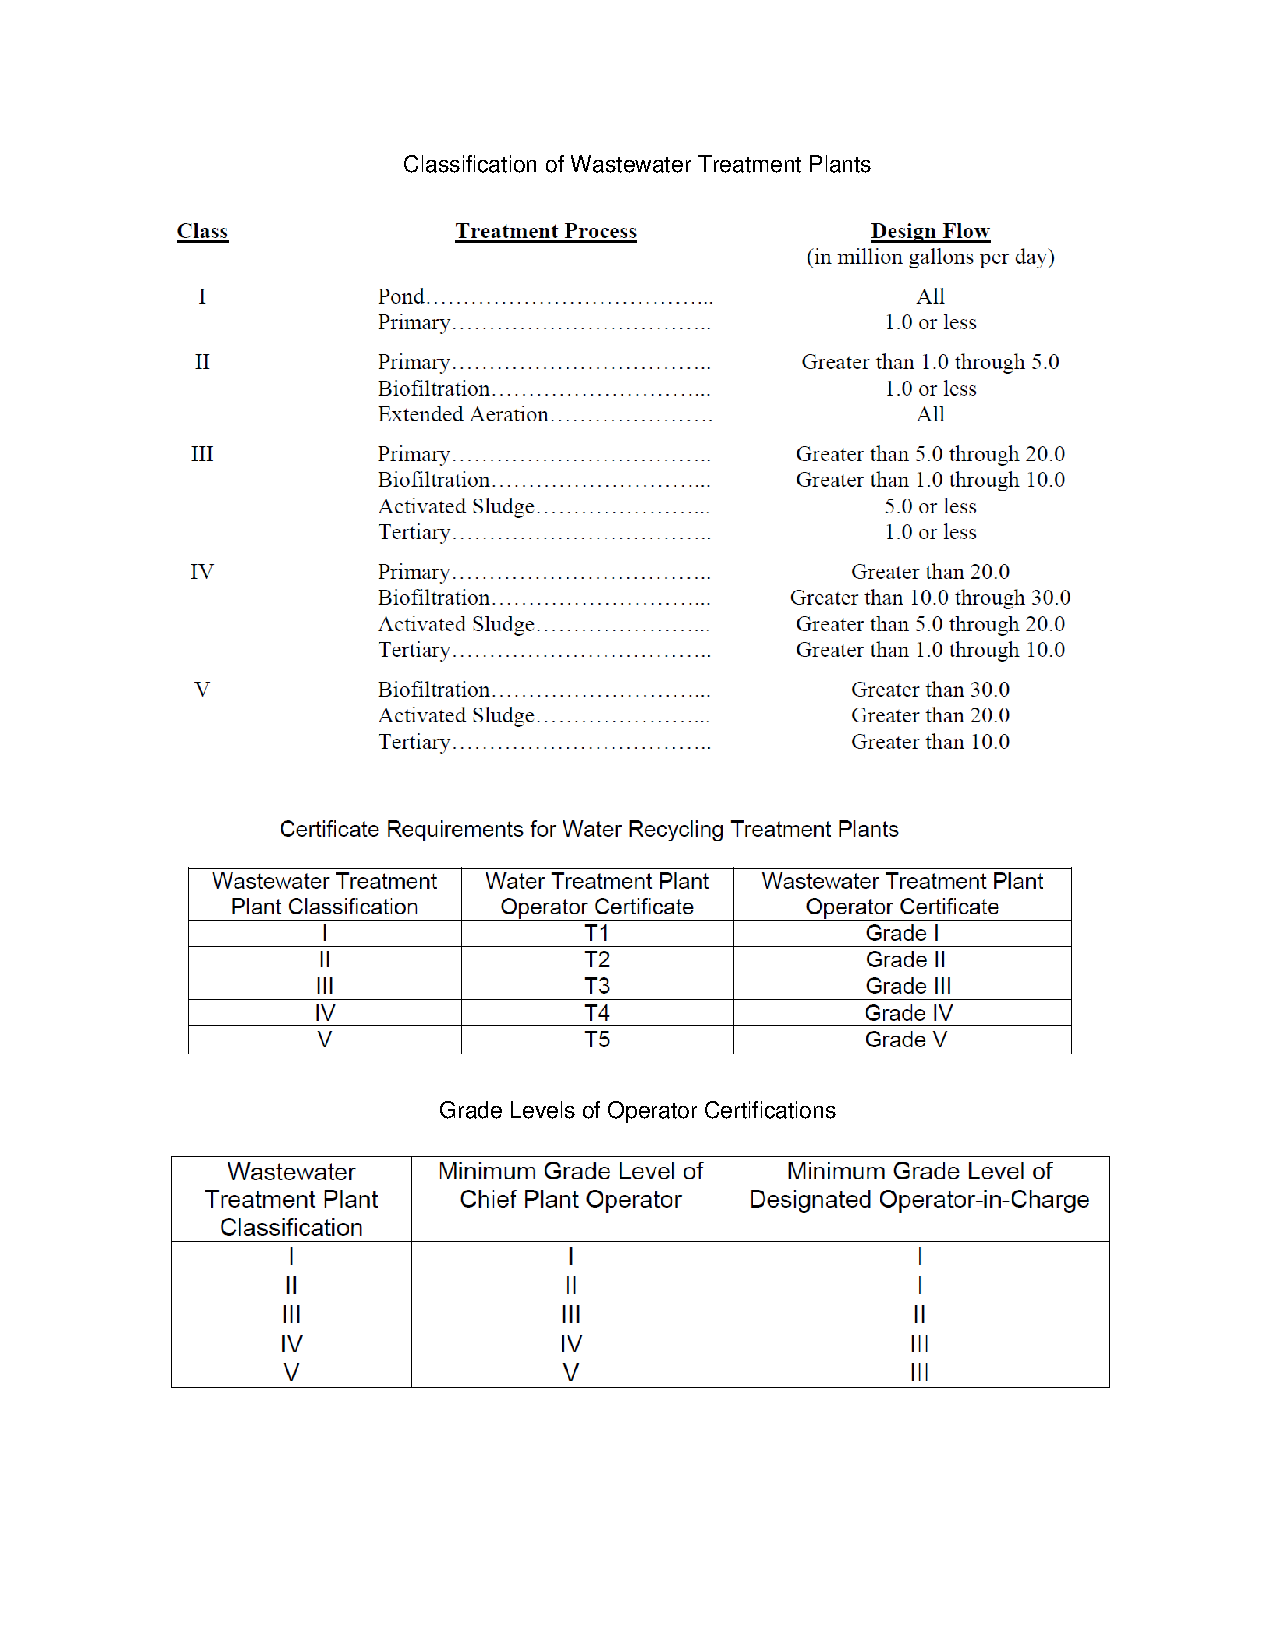
\includepdf[pages=-]{WastewaterPlantOperatorClassificationRequirements.pdf}
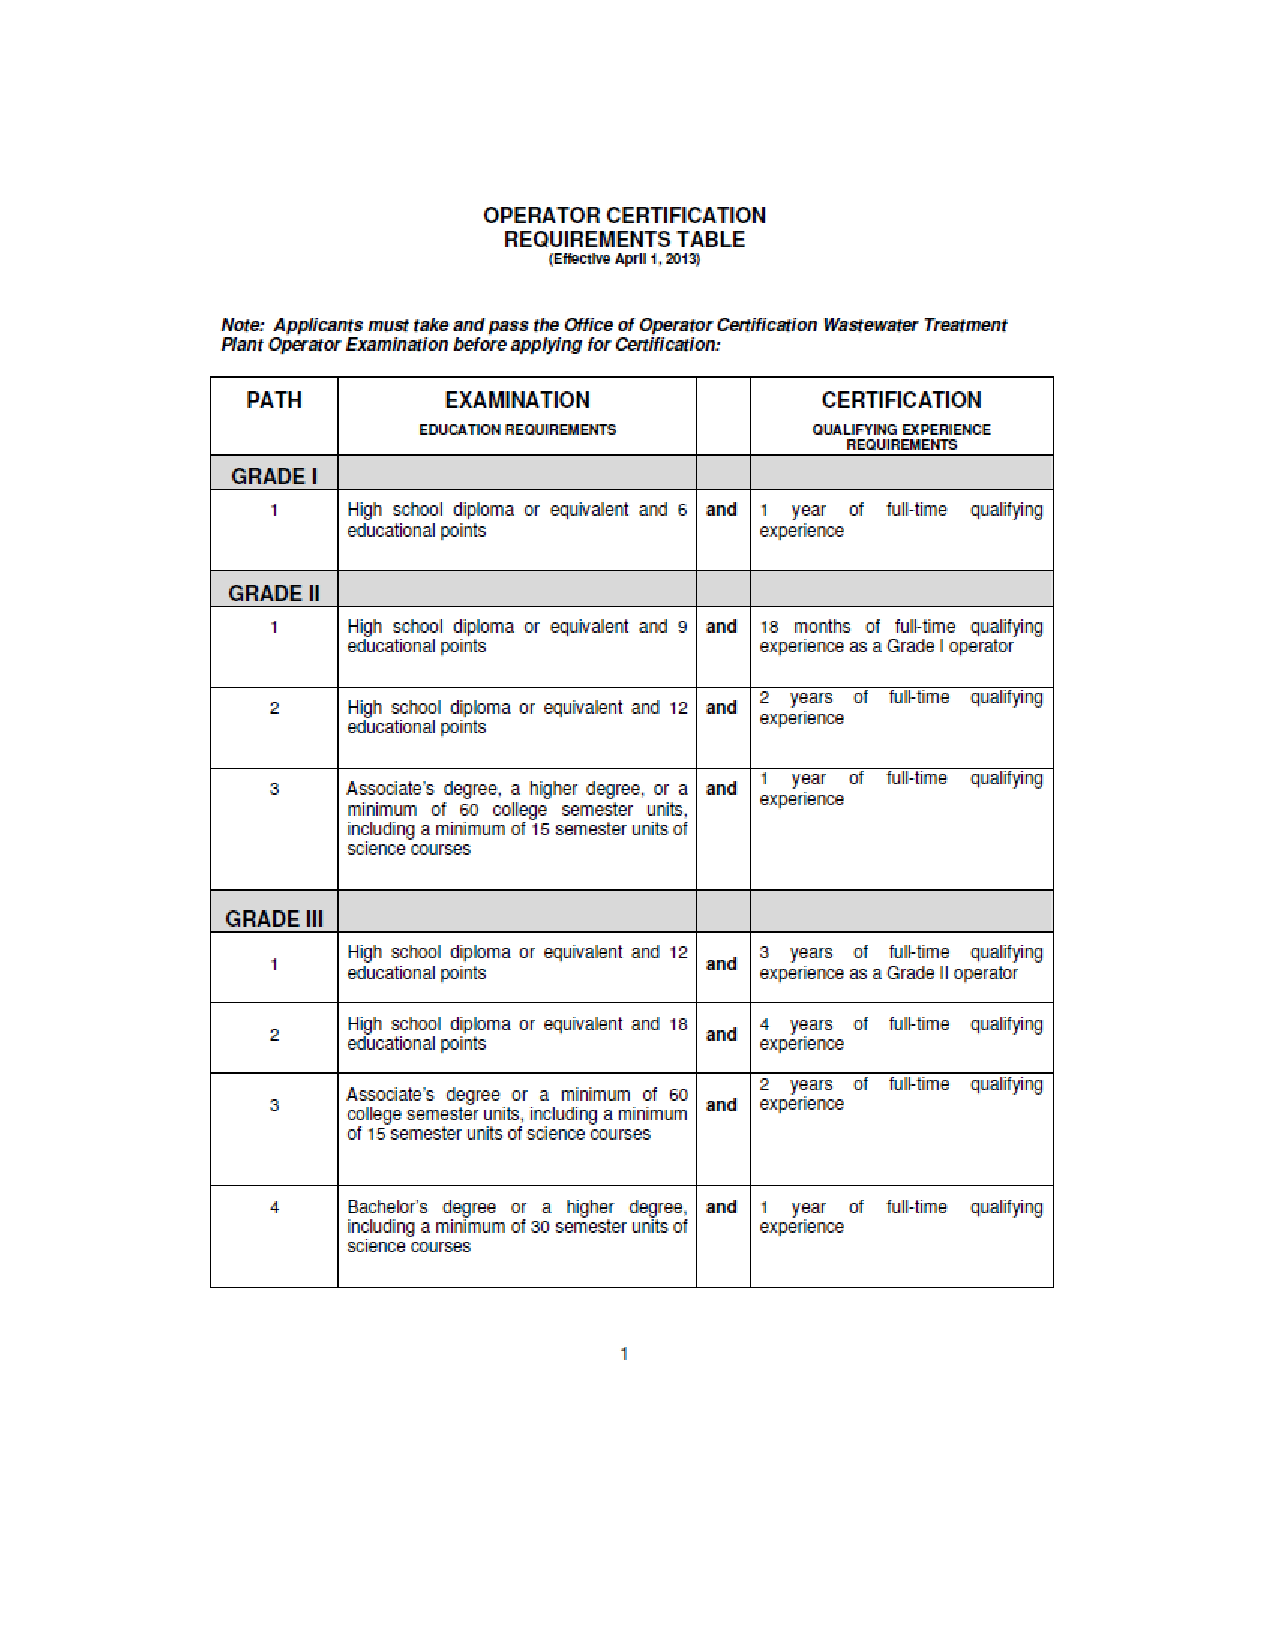
\includepdf[pages=-]{CertificationRequirement.pdf}

\subsection{Worker Safety}\index{Worker Safety}
\begin{itemize}
\item Wastewater treatment facility can be an extremely unsafe occupational field
\item It involves most of the major categories of workplace hazards:  biological, chemical, physical, safety and ergonomic,  accentuated with other factors such as shift work and diverse tasks.
\item Entities including The Occupational Safety and Health Administration(OSHA) National Electrical Code (NEC), National Fire Protection Association (NFPA), Underwriters Laboratory (UL) have recognized these hazards and implemented codes and standards to protect the affected persons and wastewater workers.
\end{itemize}

%
%\part{Module 3}
%\chapterimage{ElementsofTreatmentImg.png} % Chapter heading image
\chapter{Elements of Wastewater Treatment}

Wastewater cycle is a part of the water cycle where the water consumed as part of the normal human and industrial activity is returned back to the environment after treatment.

Wastewater cycle comprises of the following sequential elements:
\begin{enumerate}
\item Generation
\item Collection
\item Treatment
\item Disposal or reuse
\end{enumerate}

\section{Generation}\index{Generation}

Wastewater originates from domestic, industrial, commercial or agricultural activities. The characteristics of wastewater vary depending on the source. Types of wastewater include: 
\begin{itemize}
\item \hl{Domestic Sewage:}  wastewater derived principally from dwellings, business buildings, institutions, and \\
\item \hl{Industrial Sewage:}  liquid waste from industrial processes\\
\end{itemize}
Typical per person generation of wastewater in the USA is about 70-100 gallons per day

\section{Collections}\index{Collections}

\begin{itemize}
\item Wastewater is collected from its point of origin - home, businesses, industries etc. and conveyed via sewer lines to a centralized wastewater treatment facility.  
\item When the rainwater drainage is made part of the sewer system, the system is termed as \hl{Combined System}.  
\item The system where the sewage is conveyed separately from the stormwater flows is termed as \hl{Separated System}.  
\item In the Separated System, the Sanitary Sewers convey the wastewater and the Stormwater Sewer conveys the storm water flows.  
\item For the Combined System, rainstorms pose the threat of overwhelming the sewers and the treatment plant
\end{itemize}  
\begin{center}
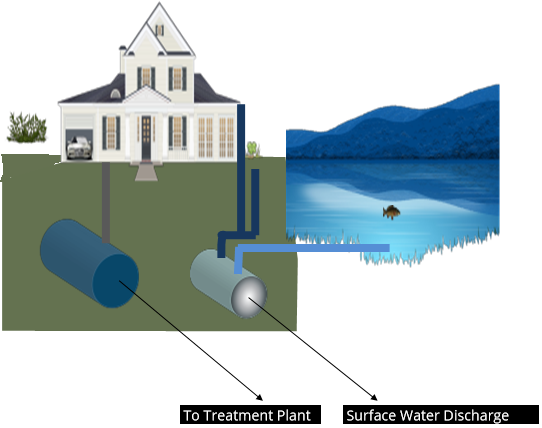
\includegraphics[scale=0.45]{SeperatedSystem1} \hspace{1 cm} 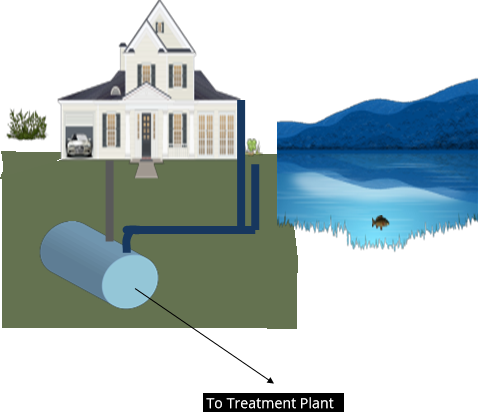
\includegraphics[scale=0.45]{CombinedSystem1}
\end{center}
			\hspace{2.6cm} Separated System \hspace{3.2cm} \parbox{\textwidth}{Combined System}\\

\section{Treatment}\index{Treatment}
\subsection{Liquid Phase Treatment}\index{Liquid Phase Treatment}
\begin{itemize}
\item Wastewater treatment can involve physical, chemical or biological processes or combinations of these processes depending on the required outflow standards. 
\item Wastewater treatment typically involves a series of steps with increasing level of treatment:
\begin{itemize}
\item \hl{Preliminary}:  The preliminary process removes large/coarse solids which include rocks, tree branches, grit and other debris present in wastewater.
\item \hl{Primary}:  The primary process is also a physical process where the separable wastewater solids - solids that float and solids that can settle, are removed.  
\item \hl{Secondary}:  Secondary treatment is a biological treatment process where microorganisms consume the organic matter present in the wastewater. 
\item \hl{Tertiary or Advanced Treatment}:  The tertiary/advanced treatment processes improve the quality of treated water beyond the secondary treatment level.  This process may include nutrient removal and disinfection.
\end{itemize}

\subsection{Treatment of Wastewater Solids}\index{Treatment of Wastewater Solids}
\begin{itemize}
\item Solids are a byproduct of wastewater treatment.  
\item Screenings and grit removed as part of the preliminary treatment is typically disposed in a landfill.
\item Sludge generated from the wastewater treatment processes -  settled solids and scum from primary and secondary treatment processes needs to be treated prior to disposal or reuse to comply with wastewater solids - biosolids regulations.
\end{itemize}

\vspace{0.5cm}
Typical solids treatment is comprised of the following three sequential steps:
\begin{enumerate}
\item Sludge thickening
\item Sludge stabilization
\item Sludge dewatering
\end{enumerate}
\vspace{0.5cm}
\subsubsection{Sludge Thickening}\index{Sludge thickening}
Sludge thickening improves performance of sludge stabilization process and provides capital and operational cost savings due to a lower volume of sludge
\subsubsection{Sludge Stabilization}\index{Sludge Stabilization}
Sludge stabilization process produces solids (biosolids) that meet Part 503 rule requirements. 
\subsubsection{Sludge Dewatering}\index{Sludge Dewatering}
Solids stabilized using digestion process has only a small percentage by weight of solids -less than 5\%.  It therefore becomes necessary to dewater the stabilized sludge prior to hauling off-site for final disposal. 
\vspace{0.5cm}
A generalized layout/process sequencing in a wastewater treatment plant is shown below:
\begin{center}
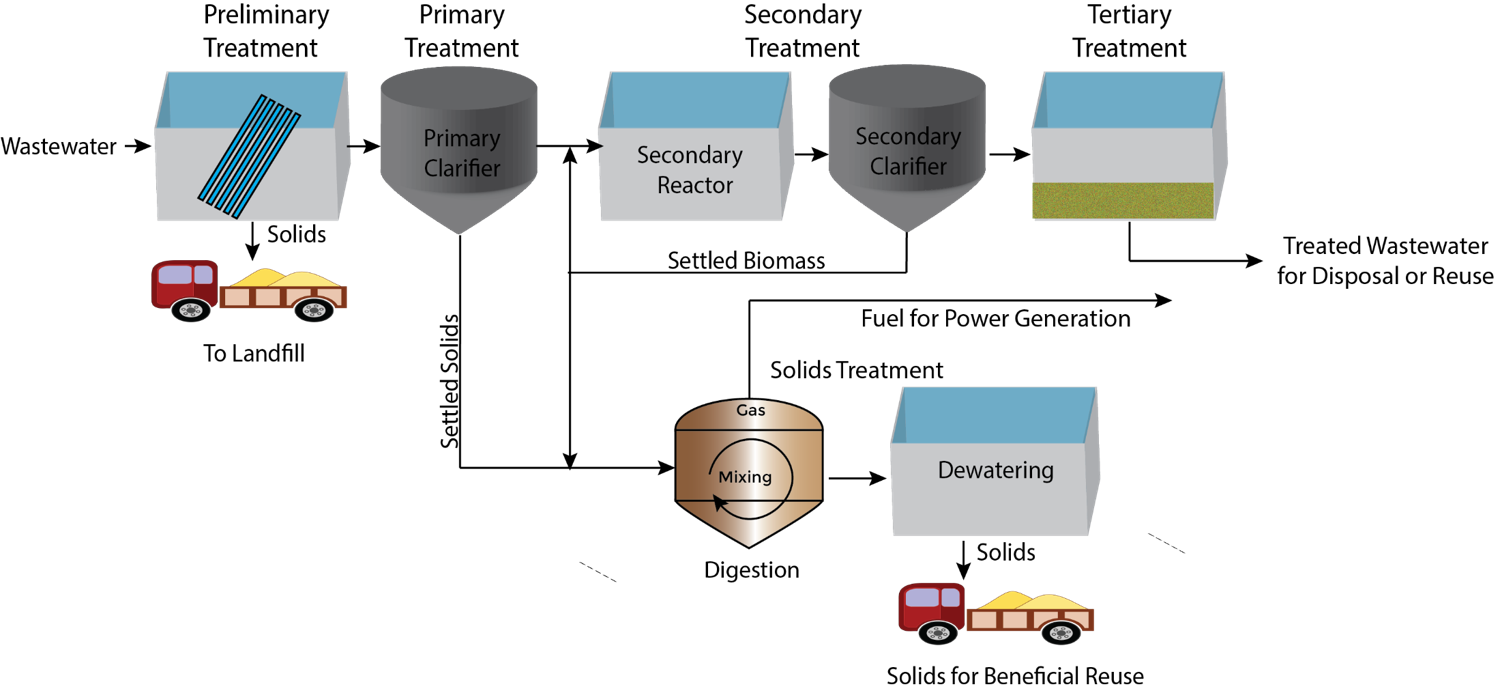
\includegraphics[scale=0.6]{TreatmentFlow}
\end{center}
Individual wastewater treatment processes involve different process options or sequences which are illustrated in the graphic below:
\begin{center}
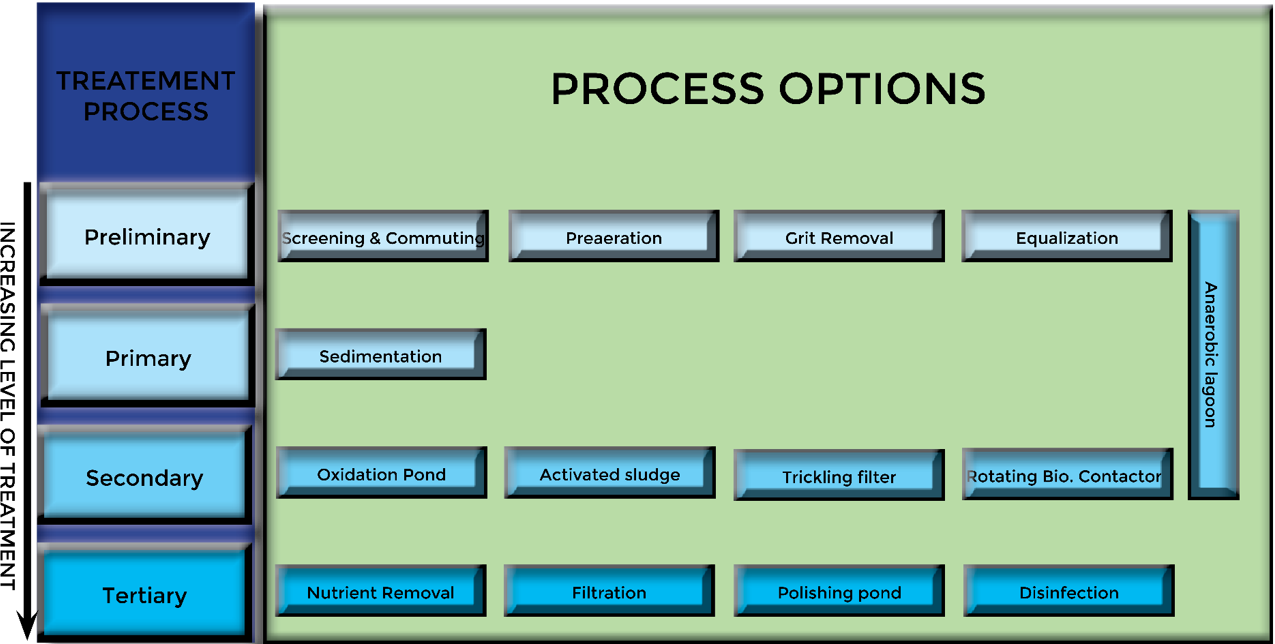
\includegraphics[scale=0.42]{Treatment}
\end{center}
\end{itemize}

\section{Disposal or Reuse}\index{Disposal or Reuse}

\begin{itemize}
\item Wastewater treatment processes can be designed to \hl{dispose} the treated water where the water is reintroduced to the environment or for \hl{reuse} where the treated water is \hl{reclaimed} or \hl{recycled} - for various purposes including irrigation, industrial use or for potable use.
\item Water disposal methods include:\\
\begin{itemize}
\item \hl{Surface water discharge}
\item \hl{Subsurface discharge}
\end{itemize}
\item Water reuse methods include:\\
\begin{itemize}
\item Potable water reuse
\begin{itemize}
\item \hl{Indirect potable reuse:}  Here the treated water is blended with groundwater or surface water and then reclaimed and treated further 
for drinking (potable) water use
\item \hl{Direct potable reuse:}  Here the treated wastewater is subjected to advanced treatment and introduced directly into a municipal water supply system
\end{itemize}
\item Water reclamation for irrigation or industrial use\\
\item Land application for beneficial use\\
\end{itemize}
\item Solids generated from the wastewater treatment process may be removed and disposed to a landfill or subject to further treatment which may allow for energy recovery - from the organic solids and for beneficial reuse due to its plant nutrient content.\\
\end{itemize}


%
%
%\part{Module 4}
%\chapterimage{Water1.png} % Chapter heading image

\chapter{Wastewater Constituents}

Domestic wastewater is 99.9\% water and the remaining 0.1\% are the pollutants that are the target for removal during the treatment process. The treatment process is designed to reduce the level of the pollutants so that the treated water does not adversely impact the environment and particularly the ecosystem of the receiving waters.

Wastewater is characterized in terms of the concentrations of the pollutants which are present in the wastewater as it is treated in the plant and in the solids produced in order to:

\begin{enumerate}
\item Monitor the quality of water, as the treatment progresses and especially that of the treated effluent to ensure treated water quality standards are met, and 
\item Allow for the the evaluation and control of the treatment processes.
\item Ensuring compliance with NPDES permits and biosolids  
\end{enumerate}

\section{Wastewater Pollutants}



Wastewater pollutants include:

\subsection{Solids}\index{Solids}
		\begin{itemize}
		\item Generally speaking wastewater solids includes feces, food particles, toilet paper, grease, oil, soap, salts, metals, detergents, sand and grit.
			\item The \texthl{solids can be classified as suspended or dissolved} based upon its ability to pass through a standardized filter paper.
			\item When the wastewater is filtered:
			      \begin{itemize}
			      	\item the residual solids remaining on the filter paper after drying in an oven at 103\si{\degree}C is the \hl{suspended solids} portion, and 
			      	\item the solids remaining after drying the filtrate are the \hl{dissolved solids}.
			      \end{itemize}
			\item Suspended solids can be categorized based upon its settling characteristics as:
			      \begin{itemize}
			      	\item \hl{Settleable}
			      	\item \hl{Non-settleable}
			      	      \begin{itemize}
			      	      	\item \hl{Colloidal}-small, charged (typically negative) particles which do not settle easily.  Some of the colloidal particles are small enough to pass through the filter paper used for filtering the suspended solids
			      	      	\item \hl{Floatable}-example oil and grease and small plastics
			      	      \end{itemize}
			      \end{itemize}
			\item Both suspended and dissolved solids can be either \hl{volatile (organic)} or \hl{fixed (inorganic)}.

			      \begin{itemize}
			      	\item The volatile solids are typically of plant or animal origin .
			      	\item The fixed solids include sand, gravel and silt as well as the dissolved salts.
			      \end{itemize}
			     \item \hl{Total Solids is thus a sum of TSS and dissolved solids or volatile and fixed solids or it can be expressed as a sum of the organic and inorganic solids.}
			      \end{itemize}

		
\subsection{Organics}\index{Organics}		
		\begin{itemize}
			\item Organics are substances containing carbon, hydrogen and oxygen, and some of which may be combined with nitrogen, sulfur or phosphorous.
			\item About 50 percent of the solids present in wastewater are organic.  This fraction is generally of animal or vegetable life, dead animal matter, plant tissue or organisms, and also include synthetic organic compounds.
			\item The principal organic compounds present in domestic wastewater are proteins, carbohydrates and fats together with the products of their decomposition.
			\item Organics are subject to decay or decomposition through the activity of bacteria and other living organisms.  \hl{Since the organic fraction can be driven off at high temperatures, they are also called \textbf{volatile solids}}.
			\item \emph{Organics in wastewater is typically quantified in terms of oxygen required to oxidize the carbon based material present} in wastewater using the \hl{Biochemical Oxygen Demand (BOD)} or \hl{Chemical Oxygen Demand (COD)} tests.
		\end{itemize}


	\subsection{Nitrogen}\index{Nitrogen}				
% 			\begin{enumerate}%@@@@@@@@@@@@@@@@@@%
% 				\definecolor{shadecolor}{RGB}{220,220,220}
% 				\begin{snugshade*}
% 					\item \noindent\textsc{Nitrogen}%@@@@@@@@@@@@@@@@@@%
% 				\end{snugshade*}

	\subsubsection{Nutrients}\index{Nutrients}	
Nitrogen and phosphorous content in wastewater is monitored as these plant nutrients, when present in wastewater effluent discharge promote growth of plant and algal matter in the receiving waters causing destruction of the normal aquatic life mainly due to oxygen depletion - eutrophication.  These nutrient from human waste (proteins are nitrogen based), food and certain soaps and detergents. 					 

\subsection{Oil and Grease}\index{Oil and Grease}	
			Fats, oil and grease in wastewater originate from homes, food establishments and industries.
			\begin{itemize}
				\item Presence of excessive oils and grease could potentially impact the secondary treatment process
				\item Oils and grease are removed as floatables in primary treatment and sent with the sludge to the digesters
			\end{itemize}


\subsection{Heavy Metals}\index{Heavy Metals}	
Heavy metals such as - Cd, Pb, Mn, Cu, Zn, Fe and Ni occur naturally in water and some of these are critical for biological growth.  Heavy metals in wastewater either remain as part of the treated wastewater or are removed as part of the wastewater solids (biosolids).  Excessive concentrations of these metals are toxic to the ecosystems of receiving waters and disposal or to the reuse sites of the wastewater solids.  The concentration threshold in the wastewater effluent are established in the facility's NPDES permit and concentrations in the metal content of the wastewater solids are controlled through the facility's compliance with Federal Biosolids Regulations (40 CFR Part 503) requirements.  Compliance with heavy metal discharge requirements are accomplished through the wastewater entities' Pretreatment or Industrial Discharge Control programs.

\subsection{Emerging Pollutants}\index{Pollutants}				
Emerging pollutants are a group of synthetic or naturally-occurring chemical or any microorganism which are not commonly monitored or regulated and are potentially known or suspected to cause adverse ecological and human health effects. These pollutants include a variety of compounds such as antibiotics, drugs, steroids, endocrine disruptors, hormones, industrial additives, chemicals, and also microbeads and microplastics. There is an inextricable link between these pollutants and wastewater.

\section{Wastewater Parameters}\index{Wastewater Parameters}			
		Laboratory and field tests are conducted to measure parameters which are critical for monitoring and controlling treatment.  The following are the key parameters that are measured.	
			
\subsection{pH}\index{pH}	
			\hl{pH is a measure of the hydrogen ion (H$^+$) content or the acidity or basicity of a solution.}  pH impacts the chemical and microbiological elements of wastewater treatment processes and thus pH measurement and control is critical.
			\begin{itemize}
				\item Pure water dissociates into equal concentration of hydrogen ions and hydroxide ions:\\ 
				      $H_2O \rightarrow H^+ + OH^-$.
				\item The H$^+$ are responsible for acidic properties and the OH$^-$ ions for the basic properties.  
				\item pH is the inverse of H$^+$ concentration; pH increases when the concentration of H$^+$ decreases relative to the concentration of OH-. 
				\item pH scale ranges from 0 – 14. When the concentration of both H$^+$ and OH$^-$ are equal, as in pure water, it is considered neutral and its pH is 7.0.  \item If the pH of a sample solution is below 7.0, the sample is termed acidic and is alkaline or basic if its pH is above 7.0. 
				\item Each change of 1 pH unit represents a 10 fold change in concentration.  For example, a sample with a pH of 2.0 is 1000 times more acidic than a sample with a pH of 5.0. 
				\item pH is measured by an electrode that is sensitive only to H$^+$ or using a pH strip which is essentially an adsorbent paper which is pre-impregnated with chemicals which change color under different H$^+$ concentrations.
				\item Most organisms involved in biological wastewater treatment processes do well within a a narrow range of pH near neutral (pH of 7).			
			\end{itemize}
			
			
\subsection{Alkalinity}\index{Alkalinity}	
			\begin{itemize}
				\item \hl{Alkalinity is the ability of a water to neutralize acids.}  
				\item During certain wastewater treatment processes including anaerobic digestion, acids are generated as a result of microbiological activity.  The bacteria and other biological entities which play an active role in wastewater treatment are most effective at a neutral to slightly alkaline pH of 7 to 8.  In order to maintain these optimal pH conditions for biological activity there must be sufficient alkalinity present in the wastewater to neutralize acids generated by the active biomass.
				\item This ability to maintain the proper pH in the wastewater as it undergoes treatment is the reason why alkalinity is so important to the wastewater industry.
				\item The alkalinity is due to the presence of acid neutralizing bases in the water including the hydroxyl (OH$^-$), carbonate (CO$_3$$^-$) and bicarbonate (HCO$_3$$^-$)  ions.  These ions are of mineral origin and are also formed from carbon dioxide which comes from the atmosphere and from the microbial decomposition of organic material.  The resistance to pH change of the water will continue until all the alkalinity contributing ions are neutralized.  
				\item The pH of a water serves as a guide to the types of alkalinity present in the water but is unrelated to the alkalinity content of a water.  Important Note:  Alkalinity is a measure of the ability to neutralize acids whereas a solution is termed alkaline (or basic) if its pH greater than 7. 
				\item Alkalinity is expressed as milligrams per liter of CaCO$_3$
			\end{itemize}
			
	
\subsection{Microbiological Characterization}\index{Microbiological Characterization}	
			
Microbiological testing and monitoring is conducted as part of the wastewater treatment for two main reasons:
	\begin{enumerate}[1.]
		\item Heterotrophic (organisms that consume organic material) microbes are responsible for the biological wastewater treatment processes - secondary treatment process, digestion and nutrient removal; 
			\begin{itemize}
				\item The effectiveness of the biological wastewater treatment processes is primarily due to the presence of a microbial ecosystem with a right balance of populations of different microbial species.
				\item Methods used for monitoring the microbial composition include direct monitoring using a light microscope to see which and how many of the different microbial species are present - typically used for activated sludge process.
				\item The microbial monitoring ensures process stability and helps identify potential process upset conditions caused by changes to the microbial population due to other external factors - toxicity, organic loading, temperature etc.
			\end{itemize}
		\item Pathogens - agents which include bacteria, viruses, protozoas and helminths that cause disease are present in wastewater effluent.
			\begin{itemize}
				\item As one of the main reasons for treating wastewater is to protect public health, microbiological/pathogen testing of the wastewater effluent and the surface water impacted by the wastewater discharge is conducted to meet the requirements of a wastewater discharge permit, to monitor the pathogen impact of treated wastewater discharge and assess the level of contamination of a public body of water.
				\item The bacteriological tests involves detection and quantification of one or more of the following bacteria:  total coliforms, fecal coliforms, E. Coli, and Enterococcus.  
					 \begin{itemize}
					      \item The main reason why these bacteria such as coliforms and enterococcus are used \hl{as it is not practical to detect and quantify all pathogens associated with wastewater.}  
					      	\item These selected bacteria originate from feces and indicate fecal contamination and thus serve as an indicator organisms for pathogens of wastewater origin.  
					      	\item Also, they are abundant, potentially less harmful, and easy to detect.  E. coli has been shown to be a better predictor of the potential for impacts to human health and therefore many newer wastewater discharge permits require E. Coli testing in lieu of fecal coliform testing requirements.
					   \end{itemize}
			\end{itemize}
	\end{enumerate}

%%
%\part{Module 5}
%\chapterimage{Water1.png} % Chapter heading image

\chapter{Wastewater Math - Part I}

\section{Units}\index{Units}

To measure any quantity or compare two physical quantities we need a universally accepted standard called Unit. The most common measurements involve measuring - length, weight and time.   International System of Units (SI), the modern form of the metric system is the globally accepted standard.  In the United States, it is customary to measure the physical quantities in English Engineering Units.\\
\vspace{0.5cm}
\begin{tabular}{c c c }
\hline
\multicolumn{3}{c}{\textbf{Fundamental Units}} \\
\hline
\textbf{Dimension} & \textbf{English Engineering Units} & \textbf{SI}\\
\hline
time & second (s) & second (s) \\
length & foot (ft) & meter (m)\\
mass & pound mass (lb) & kilogram\\
\end{tabular}\\

\vspace{0.5cm}

The measurement of any physical quantity is expressed in terms of a number - which is the quantity and a specific unit.  
Thus, a measurement of 5000 ft is basically 5000 of the of length as measured in ft.

Using the fundamental physical measurements, mathematical calculations can be made to measure other physical quantities such as area (ft$2$), volume (ft$3$), velocity (ft/s), flow (ft$3$/s), density (lbs/ft$3$).

Depending on the what is being measured or quantified, there are appropriate and customary units of measure - for example - miles and inches for length, gallons and acre-ft for volume and milligrams and tons for mass.
% \begin{enumerate}
% \definecolor{shadecolor}{RGB}{200, 200, 240}
% \begin{snugshade*}
%\section{Units and Unit Conversion}\index{Units and Unit Conversion}
% 	\item \noindent\textsc{Units and Unit Conversion}
% \end{snugshade*}
\subsection{Unit Conversions}\index{Unit Conversions}
Unit conversion is a process for changing the units of a measured quantity without changing its value.  It involves 
utilizing a \hl{conversion factor} which expresses the relationship between units that is used to change the units of a measured quantity without changing the value. Examples of conversion factors include:\\

\begin{center}
\renewcommand{\arraystretch}{1.5}
\vspace{0.5cm}
\begin{tabular}{l| c c }
\hline
\multicolumn{2}{c}{\textbf{Fundamental Units}} \\
\hline
\textbf{Dimension} & \textbf{Conversion Factor}\\[0.5cm]

\hspace{0.3cm}
time & $\dfrac{60 \enspace sec}{min}$, $\dfrac{1,440\enspace sec}{day}$\\[0.5cm]
length & $\dfrac{12 \enspace in}{ft}$, $\dfrac{5,280 \enspace ft}{mile}$\\[0.5cm]
mass & $\dfrac{2,000 \enspace lbs}{ton}$, $\dfrac{1000 \enspace gm}{mg}$\\
\end{tabular}\\
\begin{tabular}{l| c c }
\hline
\multicolumn{2}{c}{\textbf{Derived Units}} \\
\hline
\textbf{Dimension} & \textbf{Conversion Factor}\\[0.5cm]

\hspace{0.3cm}
area & $\dfrac{43,560 \enspace ft^2}{acre}$, $\dfrac{60 \enspace sec}{min}$\\[0.5cm]
volume & $\dfrac{27 \enspace ft^3}{yd}$, $\dfrac{7.48 \enspace gal}{ft^3}$\\
\end{tabular}\\
\end{center}
\vspace{0.5cm}

The numerator and the denominator of any conversion factor always equals one, they have the same value expressed in different units.

For converting one measurement unit to another.

Step 1:  Make sure the original unit is for the same measurement as the conversion unit.  So if the original unit is for area, say ft$^2$ the conversion unit can be another area unit such as in$^2$ or acre but it cannot be gallons as gallon is a unit of volume.

Step 2: Write down the conversion formula as:

$Quantity \enspace in \enspace converted \enspace unit = Quantity \enspace (\cancel{Original \enspace Unit}) *   Conversion  \enspace Factor \enspace  \dfrac{Conversion \enspace unit}{\cancel{Original \enspace unit}}$\\
\hspace{0.2cm}
Unit conversions may involve single factor where the original unit value is multiplied by the conversion factor to obtain the measured parameter in the converted (desired) unit.\\
For example:\\  
Converting 1000 $ft^3$ to cu. yards:\\

$1000 \cancel{ft^3}*\dfrac{cu.yards}{27\cancel{ft^3}} = 37 cu.yards$\\

Other unit conversions may require multiplying by known constants along with conversion factors.\\
For example:\\
\begin{enumerate}  

\item Converting 3.5 $ft^3/sec$ to MGD:\\
$\dfrac{3.5 \enspace \cancel{ft^3}}{\cancel{sec}} * \dfrac{7.48\cancel {\enspace gal}}{\cancel{ft^3}} * \dfrac{MG}{\enspace 10^6 \cancel{gal}}* \dfrac{1440*60 \enspace \cancel{sec}}{day}=  2.3 \enspace MGD$\\

\item Converting 1,000 L water to lbs:\\
$1000 \enspace \cancel{L}*\dfrac {\cancel{gal}}{3.785 \enspace \cancel{L}}*\dfrac{8.34 \enspace lbs}{\cancel{gal}}\enspace  = 2,203 \enspace lbs$\\
$(Note:8.34 \enspace lbs/gal \enspace is \enspace density \enspace of \enspace water - a \enspace constant)$\\ 

\end{enumerate}

\section{Area \& Volume}\index{Area \& Volume}
% \section{Area \& Volume}\index{Area \& Volume}

% \begin{snugshade*}
% 	\item \noindent\textsc{Area \& Volume}
% \end{snugshade*}

\begin{center}
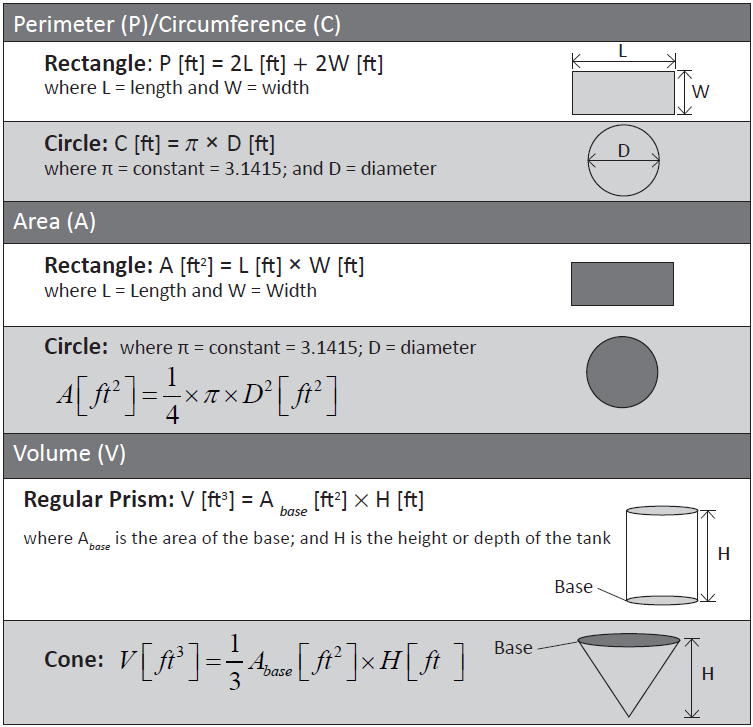
\includegraphics[scale=0.5]{Area&VolumeFormula}
\end{center}
\subsection{Example Problems}
% \hl{Example Problems}\\
\begin{enumerate}

\item The floor of a rectangular building is 20 feet long by 12 feet wide and the inside walls are 10 feet high. Find the total surface area of the inside walls of this building\\
Solution:\\
% \begin{center}
\begin{tikzpicture}
	%%% Edit the following coordinate to change the shape of your
	%%% cuboid
      
	%% Vanishing points for perspective handling
	\coordinate (P1) at (-7cm,1.5cm); % left vanishing point (To pick)
	\coordinate (P2) at (8cm,1.5cm); % right vanishing point (To pick)

	%% (A1) and (A2) defines the 2 central points of the cuboid
	\coordinate (A1) at (0em,0cm); % central top point (To pick)
	\coordinate (A2) at (0em,-2cm); % central bottom point (To pick)

	%% (A3) to (A8) are computed given a unique parameter (or 2) .8
	% You can vary .8 from 0 to 1 to change perspective on left side
	\coordinate (A3) at ($(P1)!.8!(A2)$); % To pick for perspective 
	\coordinate (A4) at ($(P1)!.8!(A1)$);

	% You can vary .8 from 0 to 1 to change perspective on right side
	\coordinate (A7) at ($(P2)!.7!(A2)$);
	\coordinate (A8) at ($(P2)!.7!(A1)$);

	%% Automatically compute the last 2 points with intersections
	\coordinate (A5) at
	  (intersection cs: first line={(A8) -- (P1)},
			    second line={(A4) -- (P2)});
	\coordinate (A6) at
	  (intersection cs: first line={(A7) -- (P1)}, 
			    second line={(A3) -- (P2)});

	%%% Depending of what you want to display, you can comment/edit
	%%% the following lines

	%% Possibly draw back faces

	\fill[gray!40] (A2) -- (A3) -- (A6) -- (A7) -- cycle; % face 6
	\node at (barycentric cs:A2=1,A3=1,A6=1,A7=1) {\tiny Floor=W*L};
	
	\fill[gray!50] (A3) -- (A4) -- (A5) -- (A6) -- cycle; % face 3
	\node at (barycentric cs:A3=1,A4=1,A5=1,A6=1) {\tiny Wall - W*H};
	
	\fill[gray!10, opacity=0.2] (A5) -- (A6) -- (A7) -- (A8) -- cycle; % face 4
	\node at (barycentric cs:A5=1,A6=1,A7=1,A8=1) {\tiny Wall - L*H};
	
	\fill[gray!10,opacity=0.5] (A1) -- (A2) -- (A3) -- (A4) -- cycle; % f2
	\node at (barycentric cs:A1=1,A2=1,A3=1,A4=1) {\tiny Wall - L*H};
	
	\fill[gray!40,opacity=0.2] (A1) -- (A4) -- (A5) -- (A8) -- cycle; % f5
	\node at (barycentric cs:A1=1,A4=1,A5=1,A8=1) {\tiny Ceiling=W*L};	
	
	\draw[thick,dashed] (A5) -- (A6);
	\draw[thick,dashed] (A3) -- (A6);
	\draw[thick,dashed] (A7) -- (A6);

	%% Possibly draw front faces

	%\fill[orange] (A1) -- (A8) -- (A7) -- (A2) -- cycle; % face 1
	\node at (barycentric cs:A1=1,A8=1,A7=1,A2=1) {\tiny Wall - W*H};
	


	%% Possibly draw front lines
	\draw[thick] (A1) -- (A2);

	\draw[<->] (-1.8,0.38) -- (-1.8,-1.3)node [midway, above=-1.8mm] {\hspace{-1.3cm}\tiny Height=10'};
	\draw[<->] (-1.6,-1.4) -- (-.3,-2.1)node [midway, above=-2.6mm] {\hspace{-1.3cm}\tiny Length=20'};
	\draw[<->] (2.6,-1.13) -- (0.2,-2.2)node [midway, below=.6mm] {\hspace{1.2cm}\tiny Width=12'};
	\draw[thick] (A3) -- (A4);
	\draw[thick] (A7) -- (A8);
	\draw[thick] (A1) -- (A4);
	\draw[thick] (A1) -- (A8);
	\draw[thick] (A2) -- (A3);
	\draw[thick] (A2) -- (A7);
	\draw[thick] (A4) -- (A5);
	\draw[thick] (A8) -- (A5);
	
	% Possibly draw points
	% (it can help you understand the cuboid structure)
%	\foreach \i in {1,2,...,8}
%	{
%	  \draw[fill=black] (A\i) circle (0.15em)
%	    node[above right] {\tiny \i};
%	}
	% \draw[fill=black] (P1) circle (0.1em) node[below] {\tiny p1};
	% \draw[fill=black] (P2) circle (0.1em) node[below] {\tiny p2};
\end{tikzpicture}\\
% \end{center}
2 Walls W*H + 2 Walls L*H= $2*12*10ft^2 + 2*20*10ft^2$\\
$=240+400=\boxed{640ft^2}$

2 Walls W*H + 2 Walls L*H + Floor + Ceiling= $2*12*10ft^2 + 2*20*10ft^2 + 2*12*20ft^2$\\
$=240+400+480=\boxed{1,120ft^2}$
\end{enumerate}
\section{Concentration}\index{Concentration}

Concentration is typically expressed as mg/l which is the weight of the constituent (mg) in 1 l (liter) of solution (wastewater).  As 1 l of water weighs 1 million mg, a concentration of 1 mg/l implies 1 mg of constituent per 1 million mg of water or one part per million (ppm).   \textbf{Thus, mg/l and ppm are synonymous.}\\  
Sometimes the constituent concentration is expressed in terms of percentage.\\
\vspace{6pt}
For example:  sludge containing 5\% solids or a 12.5\% chlorine concentration solution.\\
\vspace{6pt}
As one liter of water weighs 1,000,000 mg, one percent of that weight is 10,000 mg.  So 1\% solids implies 10,000 mg of solids per liter or 10,000 mg/l or 10,000 ppm.\\
\vspace{6pt}
$1\% concentration = 10,000 \enspace ppm \enspace or \enspace\dfrac{mg}{l}$\\
\vspace{6pt}
$0.1\% concentration = 1,000 \enspace ppm \enspace or \enspace \dfrac{mg}{l}$\\
\vspace{6pt}
$0.01\% concentration = 100 \enspace ppm \enspace or \enspace \dfrac{mg}{l}$\\
\vspace{6pt}
$10\% concentration = 100,000 \enspace ppm \enspace or \enspace \dfrac{mg}{l}$\\
\vspace{6pt}
$5\% concentration = 50,000 \enspace ppm \enspace or \enspace \dfrac{mg}{l}$\\
\vspace{6pt}
$A \enspace  12.5\% \enspace bleach \enspace solution \enspace contains \enspace 12.5\% \enspace or \enspace 125,000 \enspace \dfrac{mg}{l} \enspace of \enspace \enspace active \enspace chlorine $


%
%\part{Module 6}
%\chapterimage{Water1.png} % Chapter heading image

\chapter{Wastewater Math - Part II}


\section{Pounds Formula}



Pounds formula is used for:
\begin{itemize}
\item Calculating the quantity in pounds of a particular wastewater constituent entering or leaving a wastewater treatment process
\item Calculating the pounds of chemicals to be added\\
\end{itemize}
So if the concentration of a particular constituent (in mg/liter) and the volume or flow of wastewater is given, one can calculate the amount of that constituent in pounds using the following – Pounds Formula:
$$lbs \enspace \textbf{or} \enspace \dfrac{lbs}{day}=concentration(\dfrac{mg}{l})*8.34*volume(MG) \enspace \textbf{or} \enspace flow(\dfrac{MG}{day}(MGD)$$

\begin{figure}[h!]
\begin{center}
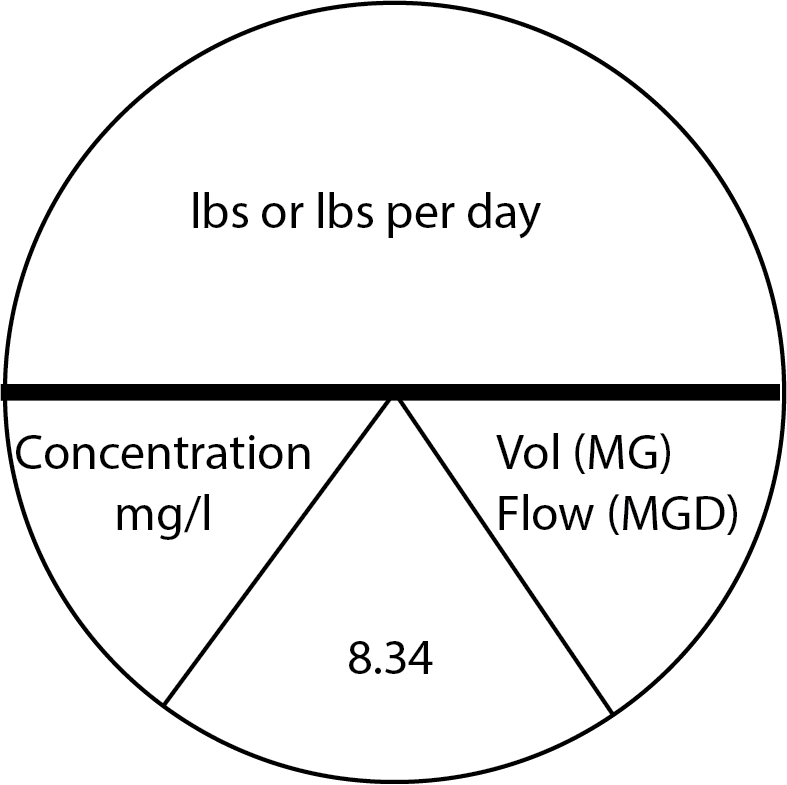
\includegraphics[scale=0.5]{PoundsFormula}
\end{center}
\caption{Pounds formula "nomograph"}
\end{figure}
\vspace{0.3cm}
There are three variables – (lbs, concentration and volume) and one constant (8.34) in the pounds formula.  Knowing any of the two variables in the formula, one can calculate the third (unknown) variable by rearranging the equation.
\subsection{Example Problems}
% \hl{Example Problems}\\
\begin{enumerate}

\item If the influent wastewater flow is 5 MGD and the BOD concentration is 240 mg/l what is the daily BOD loading in lbs/day?\\
Solution:\\
$\dfrac{lbs \enspace BOD}{day}=5MGD*240mg/l*8.34=\boxed{\dfrac{10,000lbs}{day}}$\\

\item Calculate the lbs of solids in the primary sludge if the sludge flow is 7500 gallons and the solids concentration is 4.5\%.\\
Solution\\
Applying lbs formula:\\
$lbs \enspace solids = \dfrac{7500 \enspace MG}{1,000,000} * 4.5*10,000 *8.34 = \boxed{2,815 \enspace lbs \enspace solids}$\\
\textbf{Note:}\\  
1) 7500 gallons was converted to MG by dividing by 1,000,000\\
$7500 \enspace gallons * \dfrac{1 MG}{1,000,000 \enspace gallons}$\\
2) 4.5\% was converted to mg/l by multiplying by 10,000 as 1\%=10,000mg/l

\item An operator dissolves 1,200 lbs of a chemical in 12,000 gallons of water, what is the resultant concentration in mg/l, of the chemical solution?\\
Solution:\\
$Concentration \enspace \dfrac{mg}{l}=\dfrac{lbs}{Volume \enspace MG \enspace * \enspace 8.34}$\\
$Concentration \enspace \dfrac{mg}{l}=\dfrac{1,200}{0.012 \enspace * \enspace 8.34}=\boxed{\dfrac{11,990 \enspace mg}{l} \enspace or \enspace 1.2\% \enspace solution}$\\
\textbf{Note:}\\  
1) 12,000 gallons was converted to MG by dividing by 1,000,000\\
$12,000 \enspace gallons * \dfrac{1 MG}{1,000,000 \enspace gallons}$\\
\end{enumerate}
\section{Process Removal Efficiency Calculations}\index{Process Removal Efficiency Calculations}

\begin{itemize}
\item Process removal rate or removal efficiency is the percentage of the inlet concentration removed.  
\item It is used for quantifying the pollutant removal during wastewater treatment and is established based upon the amount of a particular wastewater constituent entering and leaving a treatment process.

\item $Process \enspace Removal \enspace Rate \enspace (\%) = \dfrac{Pollutant \enspace  In-Pollutant\enspace  Out}{Pollutant \enspace In}*100$\\

\item If 10 units of a pollutant are entering a process and 8 units of pollutant are leaving (process removes 2 units), then the process removal rate for that pollutant is (10-8)/10*100=20\%.  In this example the process is 20\% efficient in removing that particular pollutant.

\item The amount of pollutant can be measured in terms of concentration (mg/l) or in terms of mass loading (lbs).  The pounds formula is used for calculating the mass loadings.  
\end{itemize}
The above example is for calculating the removal efficiency using the inlet and outlet concentrations or mass loading.\\
The methods below can be used for calculating either the inlet or outlet pollutant concentrations, if the removal efficiency and the corresponding inlet or outlet concentrations are given. 


\hl{Case 1:  Calculating outlet conc. (X) given the inlet conc. and removal efficiency (RE\%):}

\tikzstyle{block} = [rectangle, draw, fill=red!40, 
    text width=6em, text centered, rounded corners, minimum height=3em]
\tikzstyle{arrow} = [draw, -latex']
\begin{figure}[!h]
\centering
\begin{tikzpicture}[node distance =1.5cm, auto]
    \draw ++(0,0) node [block] (Process) {Process};
   \node[node distance=1.9in] (dummy_in) [left of=Process] {In};
   \node[node distance=1.9in] (dummy_out) [right of=Process] {Out};
	\node (Removal) [below of=Process, yshift=-0in] {$\tiny{Removal \enspace Efficiency=RE\% \enspace (Given)}$};
    \path [arrow] (dummy_in)-- (Process)  node [above] {\hspace{-5.8cm}$A \enspace mg/l \enspace (Given) $} node [below] {\hspace{-5.8cm}$100 \enspace mg/l$};
    \path [arrow] (Process) -- (dummy_out)  node [above] {\hspace{-4cm}$X \enspace mg/l \enspace (Unknown)$} node [below] {\hspace{-3.9cm}($100-RE\%)\enspace mg/l$};
   \draw[arrow] (Process) -- (Removal);
\end{tikzpicture}
\end{figure}
Using the fact that if the inlet concentration was 100 mg/l, the outlet concentration would be 100 minus the removal efficiency.\\
Setup the equation as:  $\dfrac{Out}{In}: \enspace \dfrac{X \enspace mg/l}{A \enspace mg/l}=\dfrac{100-RE\%}{100}$\\
Calculate X using cross multiplication - if $\dfrac{A}{B}=\dfrac{C}{D} \implies A=B*\dfrac{C}{D}$:\\
$X \enspace mg/l=A \enspace mg/l*\dfrac{100-RE\%}{100}$\\

\hl{Case 2:  Calculating inlet conc. (X) given the outlet conc. and removal efficiency (RE\%):}

\begin{figure}[!h]
\centering
\begin{tikzpicture}[node distance =1.5cm, auto]
    \draw ++(0,0) node [block] (Process) {Process};
   \node[node distance=1.9in] (dummy_in) [left of=Process] {In};
   \node[node distance=1.9in] (dummy_out) [right of=Process] {Out};
	\node (Removal) [below of=Process, yshift=-0in] {$Removal \enspace Efficiency=RE\% \enspace (Given)$};
    \path [arrow] (dummy_in)-- (Process)  node [above] {\hspace{-5.8cm}$X \enspace mg/l \enspace (Unknown)$} node [below] {\hspace{-5.8cm}$100 \enspace mg/l$};
    \path [arrow] (Process) -- (dummy_out)  node [above] {\hspace{-4cm}$A \enspace mg/l \enspace (Given)$} node [below] {\hspace{-3.9cm}($100-RE\%)\enspace mg/l$};
   \draw[arrow] (Process) -- (Removal);
\end{tikzpicture}
\end{figure}
Using the fact that if the inlet concentration was 100 mg/l, the outlet concentration would be 100 minus the removal efficiency.\\
Setup the equation as:  $\dfrac{In}{Out}: \enspace \dfrac{X \enspace mg/l}{A \enspace mg/l}=\dfrac{100}{100-RE\%}$\\
\vspace{0.3cm}
Calculate X using cross multiplication - if $\dfrac{A}{B}=\dfrac{C}{D} \implies A=B*\dfrac{C}{D}$:\\
$X \enspace mg/l=A \enspace mg/l*\dfrac{100}{100-RE\%}$\\

\vspace{0.4cm}
\hl{Example Problems:}\\

\begin{enumerate}

\item What is the \% removal efficiency if the influent concentration is 10 mg/L and the effluent concentration is 2.5 mg/L?\\
$Removal \enspace Rate (\%) = \dfrac{In-Out}{In}*100 \implies \dfrac{10-2.5}{10}*100=\boxed{75\%}$



\item Calculate the outlet concentration if the inlet concentration is 80 mg/l and the process removal efficiency is 60\%\\
Solution:\\

\tikzstyle{block} = [rectangle, draw, fill=red!40, 
    text width=6em, text centered, rounded corners, minimum height=3em]
\tikzstyle{arrow} = [draw, -latex']
\begin{figure}[!h]
\centering
\begin{tikzpicture}[node distance =1.5cm, auto]
    \draw ++(0,0) node [block] (Process) {Process};
   \node[node distance=1.5in] (dummy_in) [left of=Process] {In};
   \node[node distance=1.5in] (dummy_out) [right of=Process] {Out};
	\node (Removal) [below of=Process, yshift=-0in] {$Removal \enspace Efficiency=60\%$};
    \path [arrow] (dummy_in)-- (Process)  node [above] {\hspace{-4.39cm}$80mg/l$} node [below] {\hspace{-4.39cm}$100mg/l$};
    \path [arrow] (Process) -- (dummy_out)  node [above] {\hspace{-3.cm}$Xmg/l$} node [below] {\hspace{-3cm}40mg/l};
   \draw[arrow] (Process) -- (Removal);
\end{tikzpicture}
%\caption[MFCC]{Diagrama en bloques del cálculo de las MFCC para un frame.}
%\label{MFCC}
\end{figure}

$\dfrac{Out}{In} \enspace:\enspace\dfrac{Actual \enspace Outlet (X)}{80}=\dfrac{100-60}{100}$\\
$\implies \dfrac{Actual \enspace Outlet (X)}{80} =0.4$\\
$\implies Actual \enspace  Outlet (X) = 0.4 * 80 = \boxed{32 mg/l}$\\


\item Calculate the inlet concentration if the outlet concentration is 80 mg/l and the process removal efficiency is 60\%\\

\tikzstyle{block} = [rectangle, draw, fill=red!40, 
    text width=6em, text centered, rounded corners, minimum height=3em]
\tikzstyle{arrow} = [draw, -latex']
\begin{figure}[!h]
\centering
\begin{tikzpicture}[node distance =1.5cm, auto]
    \draw ++(0,0) node [block] (Process) {Process};
   \node[node distance=1.5in] (dummy_in) [left of=Process] {In};
   \node[node distance=1.5in] (dummy_out) [right of=Process] {Out};
	\node (Removal) [below of=Process, yshift=-0in] {$Removal \enspace Efficiency=60\%$};
    \path [arrow] (dummy_in)-- (Process)  node [above] {\hspace{-4.39cm}$Xmg/l$} node [below] {\hspace{-4.39cm}$100mg/l$};
    \path [arrow] (Process) -- (dummy_out)  node [above] {\hspace{-3.cm}80mg/l} node [below] {\hspace{-3cm}40mg/l};
   \draw[arrow] (Process) -- (Removal);
\end{tikzpicture}
\end{figure}

$\dfrac{In}{Out} \enspace : \enspace \dfrac{Actual \enspace inlet \enspace  (X)}{80}=\dfrac{100}{100-60}\implies \dfrac{Actual \enspace inlet \enspace  (X)}{80}=2.5$\\    
Rearranging the equation:   $Actual \enspace inlet (X)=2.5*80 = \boxed{200 mg/l}$\\



\end{enumerate}
%
%\part{Module 7}
%\chapterimage{Week3Clarifier1.jpg} % Chapter heading image

\chapter{Liquid Treatment Part I}

\section{Collection}\index{Collection}	
The collection system resembles a tree that branches out from the treatment plant to collect the wastewater from individual sources.

\subsection{Wastewater Collection Piping}\index{Wastewater Collection Piping}	
	\begin{itemize}
		\item A \hl{lateral} is the piping that connects the public sewer to the building. 
		\item Laterals flow into larger lines called \hl{mains}.
		\item Mains carry the flow into the largest lines in the system, called \hl{trunk lines}. 
		\item A trunk line is the pipe that brings water into the treatment plant.
	\end{itemize}
\subsection{Sanitary Sewer Systems}\index{Sanitary Sewer Systems}

Sanitary sewer systems collect and convey wastewater from residential, commercial and industrial sources to a centralized wastewater treatment facility for treatment. 

\subsubsection{Storm-water systems}\index{Storm-water systems}

Storm-water systems are designed solely for the conveyance of storm-waters waters directly to streams, rivers, lakes, or the ocean.
 
\subsubsection{Combined sewer systems}\index{Combined sewer systems}
\begin{itemize}
\item Combined sewer systems collect and convey sanitary sewage and urban runoff in a common piping system.
\item Combined sewers could potentially cause serious water pollution problems during combined sewer overflow (CSO) events when wet weather flows exceed the sewage treatment plant capacity.
	\end{itemize}
\begin{center}
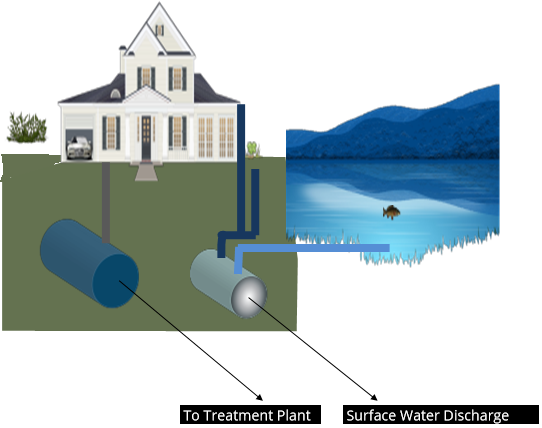
\includegraphics[scale=0.45]{SeperatedSystem1} \hspace{1 cm} 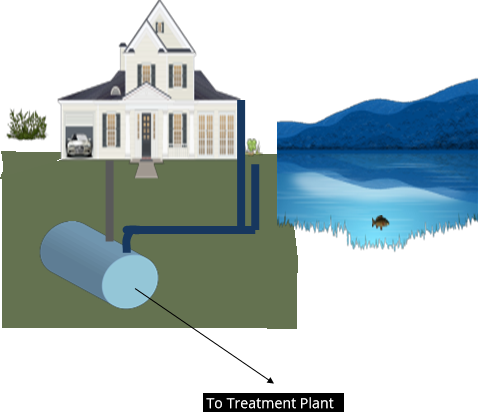
\includegraphics[scale=0.45]{CombinedSystem1}
\end{center}
			\hspace{2.6cm} Separated System \hspace{3.2cm} \parbox{\textwidth}{Combined System}\\

\subsection{Collections Systems Basics}\index{Collections Systems Basics}
	\begin{itemize}
\item The primary type of a collection system is a \hl{gravity system}. A gravity system is so named because the wastewater flows down gradient in the sewer, driven by forces of gravity. 
\item The collection system includes the gravity sewers, force mains, manholes, pumping equipment, and other facilities that collect and convey the water to a wastewater treatment plant. 
\item Sewers are generally laid at a minimum slope to ensure open channel flow through the pipe at a \hl{minimum velocity of 2.0 feet per second}. The minimum velocity is required to ensure that solids do not settle out in the sewer.  
\item When the sewer lines reach a certain depth, the flow must be lifted back through a lift or pump station.  
\item \hl{Lift stations} are built whenever wastewater must be pumped to a higher altitude, whether it's to lift water up so that it can gravity flow or to pump it over a rise or hill.  
\item The discharge from the pump station may be to another gravity sewer at that location or through a pressurized force main. 
\item Key elements of lift stations include a wastewater receiving well (wet-well), pumps and piping with associated valves.
\item The size of the wet well affects the operating of the station. If a wet well is too small, excessive starting and stopping of the pump motors will occur, resulting in premature failure. If the wet well is too large, solids will tend to settle on the bottom, blocking the pump suction line and leading to the generation of hydrogen sulfide and methane.
\item The dry well is the portion of the dry well/wet well pumping station that houses the necessary equipment required to pump the wastewater. The dry well is so named because it is isolated from the incoming wastewater.
\item Centrifugal pumps are the most common type of pump found in wastewater pumping stations. 
\item In the USA, wastewater generated in a typical home is about 70 gal/day/person
\end{itemize}


\section{Preliminary Treatment}\index{Preliminary Treatment}

			\begin{itemize}
				\item The objective of preliminary treatment is to remove coarse solids and other large materials often found in raw wastewater
				\item Removal of these materials is necessary to enhance the operation and maintenance of subsequent treatment units\\
				\item Preliminary treatment operations typically include a combination of the following processes:
					\begin{itemize}
						\item Screening
						\item Grinding or shredding
						\item Flow measurement
						\item Grit removal
						\item Pre-aeration
						\item Flow equalization
					\end{itemize}
			\end{itemize}

				
		\subsection{Process Elements of Preliminary Treatment}\index{Process Elements of Preliminary Treatment}	
			
		\subsubsection{Screening}\index{Screening}
					\begin{itemize}
						\item Screening is typically the first unit in a preliminary treatment
						\item Screening allows for the capture of coarse solids as pieces of cloths garbage so as to protect pumps and other units from clogging. 
						\item Screens may consist of vertical or inclined bars (bar racks or bar screens), wire mesh or perforated plates having either circular or rectangular openings. 
						\item Screens remove the large, entrained, suspended or floating solids such as pieces of wood, cloth, paper, plastics, garbage, etc.
						\item Debris collected on the screen can be cleaned manually or automatically using chain driven rakes 
						\item The retained material at screens - screenings, is collected and hauled to landfill for disposal
						\item The quantity of screenings removed varies by location and is a function of the clear opening of the screen.
						\item Barmuinitors combine the function of a screen and a grinder.  The ground material is returned to the wastewater flow for removal during primary treatment.
					\end{itemize}

\begin{figure}
\begin{center}
    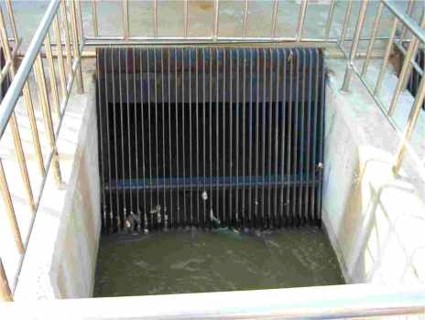
\includegraphics[width=0.7\linewidth]{Barscreen}\\

Barscreen - No rakes
\end{center}
  \end{figure}
  

		\subsubsection{Grinding and Shredding}\index{Grinding and Shredding}

					\begin{itemize}
\begin{minipage}{\textwidth}	\item Comminutor(Grinder) consist of fixed, rotating or oscillating teeth or blades, acting together to reduce the solids to a size which will pass through fixed or rotating screens grind rags into small chunks
\item The comminutors are installed in wastewater channel and they grind the larger solids without actually removing them from the wastewater.  These devices may be installed before the screens or as a combination of screen and cutters (barmunitors).
					\end{minipage}	
					\end{itemize}
					\begin{minipage}{\textwidth}
					\begin{center}
      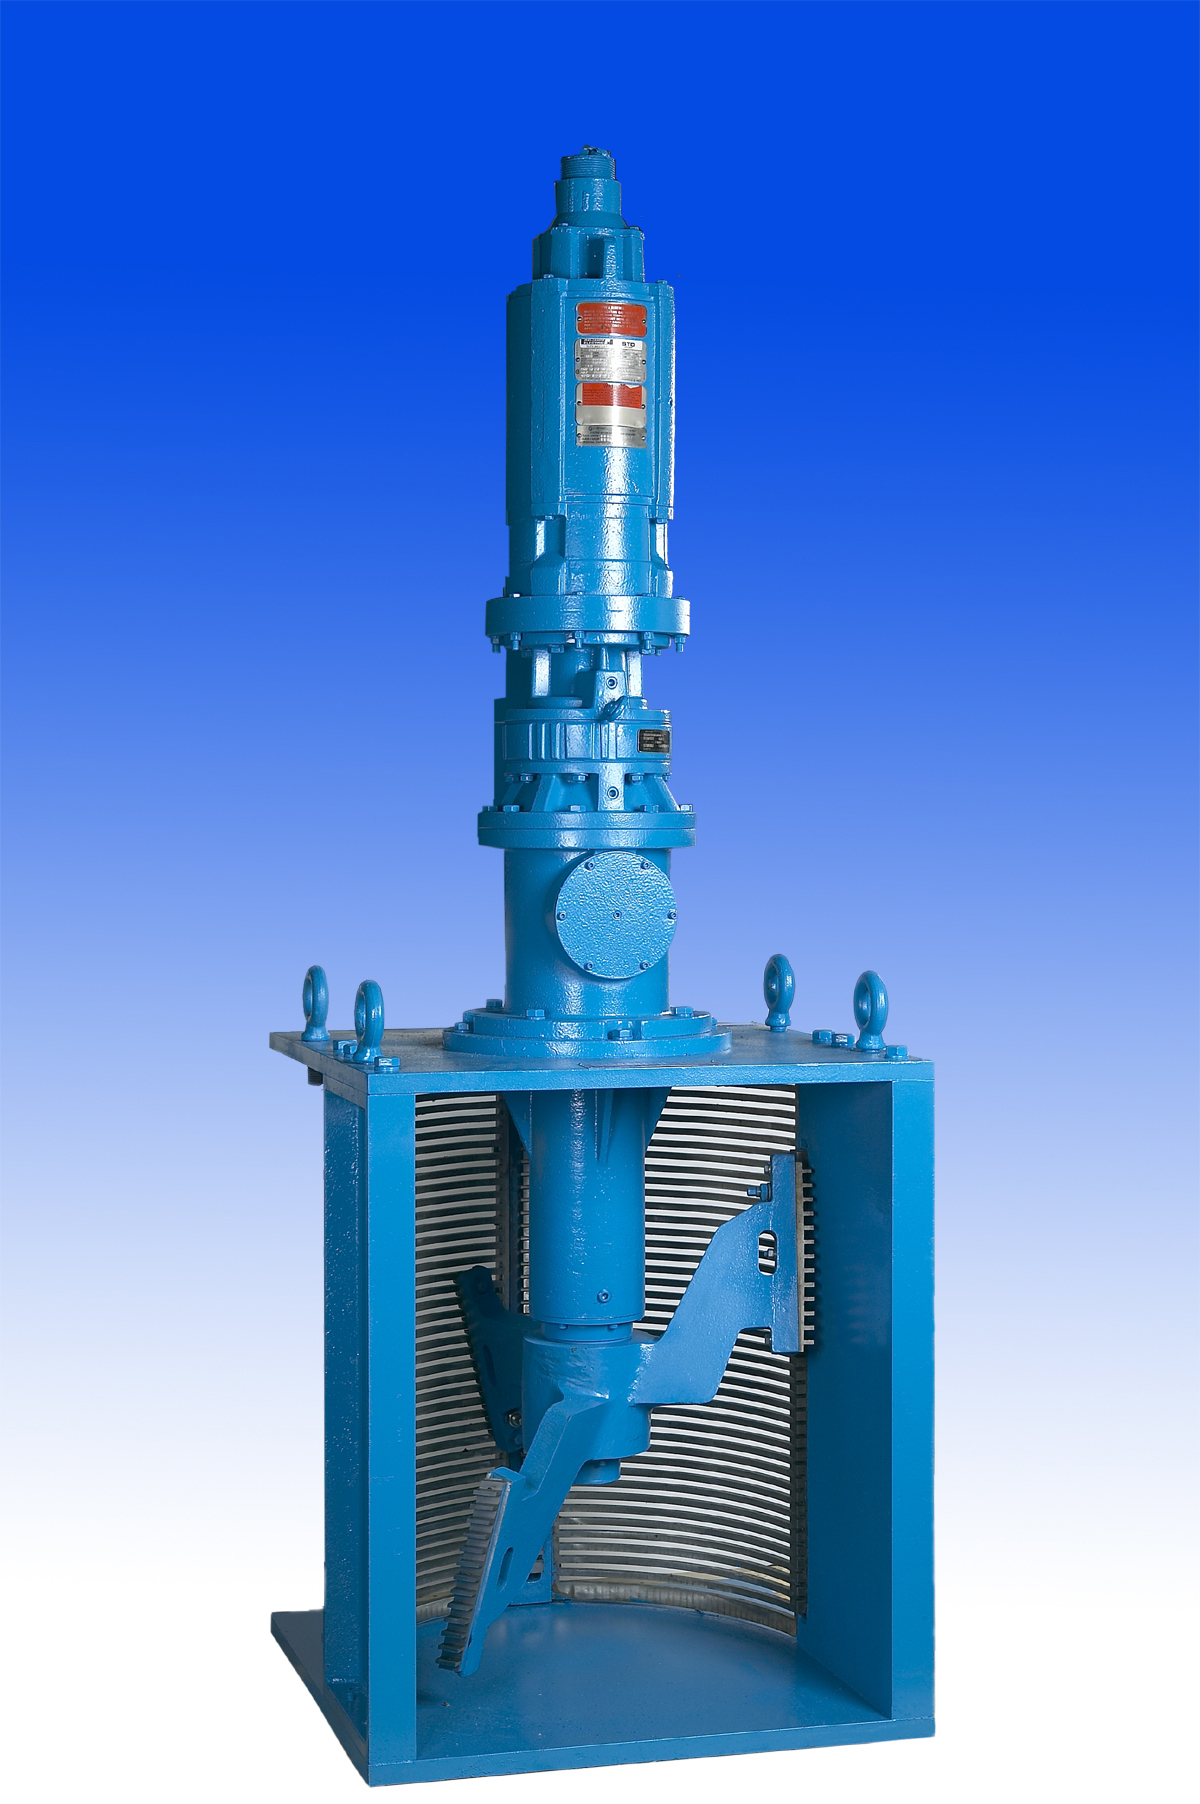
\includegraphics[width=0.3\linewidth, height=70mm]{Comminutor}\\
      Comminutor\\
\end{center}
    \end{minipage}
  
		\subsubsection{Flow Measurement}\index{Flow Measurement}
					\begin{itemize}
						\item Wastewater flow to a treatment plant is not constant but varies in a diurnal (daily) pattern reflecting domestic water use activity.
						\item Continuous flow measurement is necessary in order to monitor diurnal variations in flow which may affect treatment plant efficiency.\\
						\item Devices used for flow measurement as part of the preliminary treatment can be placed in a channel or in a pipe.
					\end{itemize}


		\subsection{Grit Removal}\index{Grit Removal}
						\begin{itemize}
							\item Grit includes sand, gravel, cinder, eggshells, bone chips, seeds, coffee grounds, and large organic particles, such as food waste.
							\item Purpose of Grit removal:
								\begin{itemize} 
									\item to protect mechanical equipment from abrasion and abnormal wear 
									\item to reduce clogging caused by deposition of grit particles in pipes and channels, and 
				\item to prevent loading the treatment plant with inert matter that might interfere with the operation of treatment units such as anaerobic digester and aeration tanks.
			\end{itemize}
		\item Removal of organic material along with the grit is undesirable for two reasons:
			\begin{enumerate}
				\item It causes odor issues, and 
				\item Organic matter is a potential source of energy (digester gas)
			\end{enumerate}
		\item Grit Disposal: Grit removed is typically landfilled.
		\item Grit Volume:  The volume of grit collected measured in ft$^3$/MG.
		\item The rate of grit collection can range from 0.5 ft$^3$/MG to 30 ft$^3$/MG.
		\item Wastewater plants having a combined collection system must deal with much larger volumes of grit.
\end{itemize}

\begin{figure}[h!]
  \centering
  \begin{subfigure}[b]{0.46\linewidth}
    \includegraphics[width=0.8\linewidth]{HorizontalGritChamber}
    \caption{Horizontal grit chamber}
  \end{subfigure}
  \hspace{0.2cm}
  \begin{subfigure}[b]{0.5\linewidth}
    \includegraphics[width=0.8\linewidth]{AeratedGritChamber}
    \caption{Aerated grit chamber}
  \end{subfigure}
\end{figure} 					

\begin{figure}[h!]
  \centering
  \begin{subfigure}[b]{0.47\linewidth}
    \includegraphics[width=0.8\linewidth]{VortexGritChamber1}
    \caption{Vortex grit chamber design}
  \end{subfigure}
  \hspace{0.2cm}
  \begin{subfigure}[b]{0.43\linewidth}
    \includegraphics[width=0.8\linewidth]{VortexGritChamber}
    \caption{Vortex grit chamber installed}
  \end{subfigure}
\end{figure} 

\subsection{Pre-aeration}\index{Pre-aeration}	
	\begin{itemize}
		\item Pre-aeration of the wastewater as part of the preliminary treatment may be provided as a separate process or increased detention time in an aerated grit chamber.
		\item Pre-aeration provides the follwoing benefits:
			\begin{itemize}
				\item freshens up wastewater by dissolving oxygen thereby reducing the wastewater septicity
				\item reduction of septicity allows for better settling - solids and BOD removal, in the following primary treatment process
				\item promotes grease separation which facilitates its removal during primary treatment
			\end{itemize}
	\end{itemize}
\subsection{Flow Equalization}\index{Flow Equalization}	

	\begin{itemize}
		\item Flow equalization involves storing a portion of peak flows for release during low-flow periods
		\item It prevents surges and allows for the operation of processes at design flows thus allowing for optimal physical, biological and chemical processes to take place.
		\item It results in saving capital costs as the processes may be built with a treatment capacity which is less than the peak flows
	\end{itemize}

\section{Primary Treatment}\index{Primary Treatment}	

\begin{itemize}
\item Synonyms:  primary treatment basin, primary clarifier, sedimentation basin, primaries, clarifier

	
		\item Primary treatment is after preliminary treatment and 				before secondary treatment
		\item Its two main objectives are: 
			\begin{itemize}
				\item Remove settleable solids
				\item Remove floatable solids
			\end{itemize}
		\item This is a physical process which relies on the physical 			properties - how heavy or light the suspended solids particles 		are to effect its separation
		\item Provides quiescent conditions for the influent 					wastewater for the heavier solids to settle and the lighter 			solids to float
		\item Removes settleable solids and floatables
		\item Settled solids are removed as sludge from the bottom of 			the clarifier
		\item Floatable solids including oil and grease are also 				removed, as scum from the surface\\
		\item The shape of the primary clarifier is either rectangular 		or circular
	
		\item Effective solids removal in the primary clarifiers will 			reduce the loading on the expensive secondary treatment 				process.
		\item The amount of solids removed during primary treatment 			may be enhanced by chemical addition - ferric or ferrous 				chloride as a coagulant and anionic polymer as the flocculant.  		This is called Chemically Enhanced Primary Treatment (CEPT).
		\begin{center}
				\includegraphics[scale=0.9]{RectangularClarifier}\\
				Cross section of a Rectangular Clarifier\\
				\includegraphics[scale=0.1]{Blank}\\
				\includegraphics[scale=0.5]{CircularClarifier3}\\
				Cross section of a circular clarifier\\
			\end{center}
				\includegraphics[scale=0.03]{Blank}\\
\item \textbf{Typical Removal Rates:}\\
\begin{itemize}
\item \hspace{10mm} BOD removal – 25\% to 40\% and about 60\% with CEPT
\item \hspace{10mm} Suspended solids (SS) removal – 40\% to 60\% and about 75\% with CEPT
\item \hspace{10mm} Settleable Solids removal - $>$90\%
\end{itemize}
\end{itemize}




%
%\part{Module 8}
%\chapterimage{Week3Clarifier1.jpg} % Chapter heading image

\chapter{Liquid Treatment Part II}

\section{Secondary Treatment}\index{Secondary Treatment}
\begin{itemize}
\item While preliminary and primary treatment processes are designed primarily to remove solids from wastewater, secondary treatment is for the removal of organics.
\item Secondary treatment involves:
\begin{itemize}
\item biological conversion of the dissolved and suspended organics in wastewater into biomass, and
\item physical settling (separation) process where the solids including the biomass formed during secondary treatment is separated and removed from the treated wastewater.
\end{itemize}

\item With the removal of gross solids in the preliminary treatment followed by removable of settleable solids in the primary clarifiers and the removal of dissolved and suspended organics in the secondary treatment processes, the wastewater is considered treated.
\item Secondary treated wastewater is typically disposed or treated further for reuse or disposal (depending upon the end use/application and the NPDES permit stipulations).
\item The solids (biomass) removed from the secondary treatment is typically mixed with the solids from primary treatment and stabilized using a solids treatment process like sludge digestion prior to its disposal.
\end{itemize}
\vspace{1cm}

\textbf{Secondary treatment process incorporates one of the following three approaches:}


\subsection{Fixed film system}\index{Fixed Film System}	
		
Trickling filter is a fixed film secondary treatment process wherein the organic content of the wastewater is removed using biological growth attached to an inert media such as lava rock or plastic\\
\begin{center}
\includegraphics[scale=0.5]{TricklingFilter}
\end{center}		
\begin{itemize}
\item In a trickling filter, the wastewater is sprayed evenly on the surface of the media with a rotary type distributor with orifices
\item The wastewater percolates through the media bed, where it comes in contact with biological slime growth – zoogleal film (zooglea)
\item The aerobic biomass - bacteria, protozoa and other microoorganisms in the zooglea capture and consume the suspended and dissolved organics from the wastewater.
\item The microorganisms metabolize the organics and in the process produce more microbial mass resulting in increasing the thickness of the zoogleal layer.
\item The thickness of the zoogleal layer can only increase to a point until the wastewater flow – hydraulic load, shears the slime layer – “sloughs off” and is carried out as part of the effluent flow as sloughing.
\item The treated wastewater cascades from the bottom of the media into the underdrain system – lower portion of the TF comprised of columns which support the media base.  The underdrain has a sloping floor to direct the cascading water into a center channel .
\item The clarifier allows for the separation (settling) of the  of the solids (sloughed off material).  The settled solids is removed - typically pumped to a digester and the clarified effluent flows out of the clarifier.
\item The source of oxygen to support the aerobic growth is from the oxygen dissolved in the wastewater as it is sprayed over the media and from the air currents due to the downward flow of the wastewater and the temperature difference between ambient and the interior of the trickling filter.  Forced ventilation system may be designed as part of the trickling filter

\item Word trickling “filter” is a misnomer - no filtration is involved
\item Advantage includes process simplicity and lower costs
\item Disadvantage include BOD removal efficiency of only about 80-85%
\item The media may be rock, slag, coal, bricks, redwood blocks, molded plastic, or any other sound durable material.
\item The media depth ranges from about three to eight feet for rock media trickling filters and 15 to 30 feet for synthetic media.
\item The media needs to be uniformly sized and have adequate empty spaces (voids) to ensure maintaining aerobic condition necessary for the survival of biomass.  

\item Pre-fabricated (synthetic) media - similar to the one shown below, has an advantage over the "dumped" type media such as lava rock of providing a greater surface area per volume upon which the zoologeal film may grow while providing ample void space for the free circulation of air.

\item Sometimes, due to inadequate hydraulic loading, portions of the zoogleal layer may become too thick and oxygen cannot penetrate its full depth, causing odor issues.





\end{itemize}



\subsection{Suspended Growth System}\index{Suspended Growth System}
\begin{itemize}
\item In this type of secondary treatment, the microbes are suspended in the
wastewater flow being treated. 
\item Air or oxygen is supplied to maintain an aerobic environment and to keep the microorganisms in suspension. 
\item Example of this secondary treatment approach include the activated sludge treatment process 
\end{itemize}

\subsubsection{Elements of Activated Sludge Process}\index{Elements of Activated Sludge Process}

\begin{center}
\includegraphics[height=4.5cm]{ASProcess}
\end{center}
\begin{itemize}

\item Utilizes an aeration basin/reactor and a secondary clarifier

\item In the presence of oxygen, aerobic bacteria in the aeration basin consume the organic matter (BOD) in wastewater for their growth and reproduction, converting BOD into bacterial cell mass along with metabolic byproducts including carbon dioxide and water

\item The aerobic bacteria is the predominant microbial life form in the aeration basin.  Other higher microbial life forms — mainly protozoa, are present along with some metazoans.

\item The microorganisms along with their metabolic byproducts and residual dead cell mass form a cluster called floc.

\item The wastewater exiting the aeration basin enters a clarifier where the floc settles.  The clear, treated secondary effluent flows out.

\item A portion of the settled activated sludge floc, is returned from the clarifier to the front of the aeration basin to seed the activated sludge treatment of the incoming primary effluent. The recycled floc is called \textbf{Return Activated Sludge (RAS)}.

\item The remaining settled floc from the clarifier is ”wasted” \textemdash transferred for solids treatment (typically using digestion) prior to its ultimate disposal. The wasted floc is called \textbf{Waste Activated Sludge (WAS)}.

\item The color of healthy activated sludge is tan to brown with an earthy/musty odor.

\item For activated sludge treatment to be effective, it is critical to establish a healthy microbial population which \hl{converts the BOD} into \hl{easily separable biomass.}
\item If the biomass does not settle well in the clarifier, it will be carried out in the treated secondary effluent producing a poor quality effluent with higher solids and organic content.  \\
\end{itemize}


\subsection{Pond System}\index{Pond System}
Similar to the suspended growth, stabilization ponds are large man made bodies of water which treat wastewater using mainly natural processes including sunlight, algae and microorganisms.
\begin{itemize}
\item Stabilization ponds and lagoons are bodies of water which treat wastewater using mainly natural processes including sunlight, algae and microorganisms for treating wastewater\\
\item While ponds are shallow and man-made, lagoons are bodies of water confined within natural boundaries.\\
\end{itemize}

 , which break down the effluent. It is in the anaerobic pond that the influent begins breaking down in the absence of oxygen "anaerobically". The anaerobic pond acts like an uncovered septic tank. Anaerobic bacteria break down the 

\subsubsection{Anaerobic Ponds}\index{Anaerobic Ponds}	

\begin{itemize}	
\item Typically for treating raw sewage
\item These are deep - 10-14 feet treatment ponds which rely primarily on anaerobic bacteria to break down the organic waste.
\item Designed for BOD removal
\item High strength wastewater may be treated.
\item Organic matter is broken down releasing releasing methane, carbon dioxide and odorous gases including hydrogen sulfide. 
\item Most of the decomposition is accomplished by acid forming bacteria. 
\item The pH in these lagoons is usually below 6.5. 
\item They are total retention and do not have an effluent discharge. 
\item The anaerobic pond must be de-sludged approximately once every 2 to 5 years
\item Organic loading of 200-1000 lbs. $BOD_5$ per acre per day
\end{itemize}

\subsubsection{Facultative Ponds}\index{Facultative Ponds}	

\begin{itemize}
\item The depth of facultative ponds is about 4-7 feet which is in-between the depths of anaerobic ponds (10-14 feet) and aerobic ponds 3 feet)
\item The uper layer of facultative pond is aerobic, and bottom layer is mostly anaerobic.
\item Facultative bacteria are responsible for most of the treatment that occurs in these ponds.  Facultative bacteria are bacteria which can live under both aerobic and anaerobic conditions.
\item The algae that grow in the pond are critical to the successful stabilization of the organic load. 
\item The algae will take in carbon dioxide ($CO_2$) and, through photosynthesis, use it to create sugars and release dissolved oxygen ($O_2$) that is used by the aerobic bacteria. Facultative lagoon levels should always maintain at least 4 feet of water in the pond.
\item Typically for secondary treatment - BOD removal
\item 15-50 lbs $BOD_5$ per acre per day.
\item Unused CO$_2$ will react with water to form carbonic acid - which would reduce the pH unless consumed
\item Sludge removal need is rare.  Sludge can be removed by using a raft-mounted sludge pump or by draining and dewatering the pond and removing the sludge with a front-end loader.
\end{itemize} 

				\begin{sidewaysfigure}
\begin{center}
\includegraphics[scale=0.8]{StabilizationPond}\\
Facultative pond schematic
\end{center}
				\end{sidewaysfigure}
				
\subsubsection{Aerobic Stabilization Ponds}\index{Aerobic Stabilization Ponds}
	
Aerobic stabilization ponds are also known as: \hl{maturation}, \hl{polishing} or \hl{finishing} Pond
\begin{itemize}
\item Contain disssolved oxygen throughout entire depth of the pond.
\item Treatment is accomplished through the stabilization of organic wastes by aerobic bacteria and algae.
\item Typically for tertiary treatment
\item Designed for pathogen removal
\item Shallow - only about 3 feet deep. 
\item They are most often the final cells in a multi-staged pond system
\item They are also used as polishing ponds for tertiary treatment of trickling filter plant effluent.
\item Usually the effluent is directed into a second pond where the sludge can settle 
\item Their shallow depth allows sunlight to penetrate to the bottom of the pond to encourage algae growth and aerobic conditions throughout the pond 
\item The low solids loading found in these tertiary treatment applications means that these ponds normally have no sludge zone
\item These ponds may be mechanically aerated 
\item Aerobic polishing ponds are designed for 15-20 pounds BOD/acre/day
\item Aerobic ponds are typically designed for pathogen removal
\item Aerobic lagoon levels should always maintain at least 18 inches of water in the pond
\end{itemize}




%
%\part{Module 9}
%\chapterimage{Dewatering.jpg} % Chapter heading image

\chapter{Solids Treatment}

\section{Why do we need to treat wastewater solids?}\index{Why do we need to treat wastewater solids?}

\begin{itemize}
\item Sludge is generated from the wastewater treatment processes -  settled solids and scum from primary and secondary treatment processes
\item This sludge contain organic compounds and also elements that are beneficial plant nutrients
\item However, the organic solids in the sludge are not stable (i.e. they will decay) and include pathogens.  \item Prior to disposal, sludge has to be treated – stabilized, so that its disposal or reuse does not pose a threat to public health.
\item Sludge treatment is very critical as it is an expensive process and sludge disposal is subject to strict regulatory requirement.
\item Even solids are only a small component of wastewater, the solids treatment and disposal account for a very substantial portion of wastewater treatment costs.  Typically 40 to 60\% of total wastewater treatment operations cost is attributable to sludge treatment and disposal.
\end{itemize}

\textbf{NOTE: Solids removed during Preliminary Treatment, from barscreens and grit chambers are typically not treated as part of the solids treatment process.  These solids are disposed off at a landfill}

\vspace{0.5cm}
\textbf{Typical solids treatment is comprised of the following three sequential steps:
\begin{enumerate}
\item Sludge thickening
\item Sludge stabilization
\item Sludge dewatering
\end{enumerate}}
\vspace{0.5cm}
\section{Sludge thickening}\index{Sludge thickening}
Sludge thickening involves the removal of excess water from the primary and secondary sludge increasing the solids content of the sludge and reducing the volume of sludge to be treated in the sludge stabilization process.
Sludge thickening reduces the volume of sludge that need to be handled in the sludge stabilization step thereby reducing treatment cost.  
\begin{itemize}
\item There is an upper limit of the solids concentration that can be effectively treated (stabilized) as increasing the solids concentration reduces its ability to be mixed and pumped easily.  Typically the sludge thickening process produces sludge with a solids content of less than 10\%.\\
\end{itemize}
Benefits of thickening to the sludge stabilization process include:
\begin{itemize}
\item Improved performance due to a lower volume of sludge
\item Cost savings in the construction of new facilities
\item Reduction in energy requirements as less water has to be heated
\end{itemize}
Typical methods used for sludge thickening include:
\begin{enumerate}
\item Gravity thickener - more suitable for primary sludge
\item Dissolved air floatation thickener - more suitable for lighter, fluffier floc such as the secondary sludge.
\end{enumerate}
\section{Sludge Stabilization}\index{Sludge Stabilization}
\textbf{}\\
Sludge stabilization process produces solids that are deemed safe for eventual disposal.  Federal Part 503 rule establishes requirements for the final use or disposal of sewage sludge.  The solids disposal methods may include: land application, as a crop/vegetation fertilizer, placed on a surface disposal site for final disposal and fired in an incinerator.\\
\textbf{Biosolids is the term used for stabilized sludge which meets regulatory standards for beneficial reuse}\\  

Sludge stabilization process results in the following:
\begin{enumerate}
\item Reduction in amount of solids
\item Pathogen reduction
\item Odor reduction
\item Reduction in vector attraction
\end{enumerate}
The main processes involved in sludge stabilization include:
\begin{itemize}
\item Digestion - Aerobic or anaerobic
\item Lime or alkaline stabilization
\item Composting
\item Long term storage in lagoons
\item Thermal processes
\item Incineration
\end{itemize}

Most common processes involved in sludge stabilization include:

		\begin{enumerate}
		\item Digestion - Aerobic or anaerobic
		\item Lime or alkaline stabilization
		\item Composting
		\item Long term storage in lagoons
		\item Thermal processes
		\item Incineration
		\end{enumerate}
		\begin{itemize}
		\item \hl{Sludge digestion is a microbiological process and is the most common sludge stabilization method}.
		\item There are two major sludge digestion processes:
			\begin{itemize}
			\item aerobic digestion which utilizes aerobic microorganisms, and produces carbon dioxide as a byproduct
			\item anaerobic digestion which utilizes anaerobic microorganisms and it produces digester gas as a byproduct.
			\item Digester gas is typically composed of 60-65\% methane gas with the remainder being mostly carbon dioxide ($CO_2$) and is useful because of its potential use as fuel - energy recovery from wastewater.
			\end{itemize}
		\end{itemize}

\subsection{Anaerobic Digestion Process Basics}\index{Anaerobic Digestion Process Basics}

		\begin{itemize}
		\item Solids removed from the primary and secondary treatment processes is fed to the digesters.  
		\item The sludge feed to the digesters range between 3 – 6\% total solids which typically contain 70\% organic solids
		\item The anaerobic digester is typically a large cylindrical concrete tank and is operated as a continuous process at a fixed volume\\ $\implies$ as sludge is fed into the digester it displaces an equal amount of sludge which leaves the digester.
\begin{center}
\includegraphics[scale=0.50]{DigesterFixedCover}\\
\textbf{Anaerobic Digester}\\
\end{center}
		\item The sludge typically occupies 70 - 90\% of the total digester volume and the methane carbon dioxide gas mixture occupies the headspace from where it is withdrawn also on a continuous basis.
		\item In the anaerobic digestion process microorganisms convert volatile matter into mainly methane (CH$_4$) and carbon dioxide (CO$_2$)
		\item The sludge content of the digesters is kept mixed and maintained in a constant temperature range using external heating.
		\item The activity and type of bacteria present in the digester is dictated by the operating temperature of the digester.
		\item Anaerobic digestion can be in the following three temperature ranges, each of which has its own unique microbiology.\\
			\begin{enumerate}[1. ]
			\item Psychrophilic digester:  Digester is maintained between 50  - 65 F.  Sludge detention time - 50 to 180 days
			\item Mesophilic digesters: – Digester is most commonly operated  between 95 – 98 F and the typical number of days required for digestion is between 15 to 30 days.\\
			\item Thermophilic digesters:  These digesters’ optimal operating temperatures range is between 113   135 F and it typically requires 5 to 12 days.\\
			\end{enumerate}     
		\item These organic solids are measured as volatile solids (VS).  
		\item The volatile solids content of the sludge entering and leaving the digester are measured to quantify the solids removal in the digester
		 \item Breakdown of volatile matter in the sludge ultimately into methane (CH$_4$) and carbon dioxide (CO$_2$) occurs in multiple steps involving different groups of microorganisms as follows:\\
			\begin{enumerate}[Step 1.]
			\item Hydrolysis:  Here the microorganisms breakdown complex organic matter in the sludge - carbohydrates, proteins, lignin, and lipids into simpler compounds including sugars, soluble fatty acids and amines.\\
			\item Acid Formation:  The simpler compounds formed in Step 1 are converted to organic acids by acid forming bacteria\\
			\item Methane Formation: The organic acids formed in Step 2 are converted into methane and carbon dioxide by methane forming bacteria.\\
			\end{enumerate}
		\item Gas production ranges between 10 to 16 cubic feet per pound of volatile matter destroyed and the gas production remains stable over time.
		\item Low gas production indicates problems - toxicity, temperature, volatile acid to alkalinity ratio, mixing, or feed rates.
		\end{itemize}


\section{Sludge Dewatering}\index{Sludge Dewatering}
Solids stabilized using digestion process has only a small percentage by weight of solids -less than 5\%.  It therefore becomes necessary to dewater the stabilized sludge prior to hauling off-site for final disposal.  Like thickening, the dewatering process does not treat the sludge.  It increases the solids content to between 15 to 30 percent and the higher solids content of the stabilized sludge makes it easier to handle and reduces costs associated with elements related to accomplishing the end objectives with the sludge – land application, composting, drying, incineration or landfill.\\
Dewatering involves conditioning the sludge with a polymer and subjecting it to a physical process which include:
\begin{enumerate}
\item Belt Filter Press 
\item Centrifuge
\end{enumerate}


%% \section{Theorems}\index{Theorems}
%\part{Module 6}
%\chapterimage{Water1.png} % Chapter heading image

\chapter{Wastewater Math - Part II}
\chapterimage{MathCover.png} % Chapter heading image
\chapter{Wastewater Math}


% \begin{enumerate}
% \definecolor{shadecolor}{RGB}{200, 200, 240}
% \begin{snugshade*}
%\section{Units and Unit Conversion}\index{Units and Unit Conversion}
% 	\item \noindent\textsc{Units and Unit Conversion}
% \end{snugshade*}
\section{Unit Conversions}\index{Unit Conversions}
Common Units:\\

Length:  inches, ft, miles\\

Area:  ft$^2$, acres \\

Volume:  ft$^3$, gallons, acres-ft.\\

Density:  weight per volume, lbs/ft$^3$, lbs/gallon\\

Flow:  ft$^3$/min, MGD, acres-ft/day\\

		


Powers of Ten

\begin{center}
    
   
    \begin{tabular}{ | c | p{4cm} | c |p{8cm}|}
    \hline

%\hline
%\multicolumn{4}{|c|}{\textbf{ESSAYS}} \\
%\hline
%\thead{A Head} & \thead{A Second \\ Head} & \thead{A Third \\ Head} \\
%\hline%

$10^{12}$ & 1,000,000,000,000 & Tera & Like in tera byte drive - trillion\\
\hline 
$10^{9}$ & 1,000,000,000 & Giga & Like in giga byte data - billion\\
\hline
$10^{6}$ & 1,000,000 & Mega & Like in mega bytes or megawatts - million\\
\hline 
$10^{3}$ & 1,000 & Kilo & Like in kilogram \\
\hline 
$10^{0}$ & 1 &  & \\
\hline 
$10^{-3}$ & 0.001 & milli & Like in millimeter - thousandth of a meter\\
\hline 
$10^{-6}$ & 0.000001 & micro & Like in microgram - millionth of a gram \\
\hline 
$10^{-9}$ & 0.000000001 & nano & Like in nanometer - billionth of a meter\\
\hline 


    \end{tabular}
    
    \end{center}


For converting one measurement unit to another.

Step 1:  Make sure the original unit is for the same measurement as the conversion unit.  So if the original unit is for area, say ft$^2$ the conversion unit can be another area unit such as in$^2$ or acre but it cannot be gallons as gallon is a unit of volume.

Step 2: Write down the conversion formula as:

$Quantity \enspace in \enspace converted \enspace unit = Quantity \enspace (\cancel{Original \enspace Unit}) *   Conversion  \enspace Factor \enspace  \frac{Conversion \enspace unit}{\cancel{Original \enspace unit}}$


\section{Example Problems}
Problem 1\\
Convert 1000 $ft^3$ to cu. yards\\

$1000 \cancel{ft^3}*\frac{cu.yards}{27\cancel{ft^3}} = 37 cu.yards$

Problem 2\\
Convert 10 gallons/min to $ft^3$/hr\\

$\frac{10 \cancel{gallons}}{\cancel{min}}*  \frac{ft^3}{7.48 \cancel{gallons}}  * \frac{60 \cancel{min}}{hr}   = \frac{80.2ft^3}{hr}$


Problem 3\\
Convert 100,000 $ft^3$ to acre-ft.\\
$100,000 \cancel{ft^3} * \frac{acre-ft}{43,560 \cancel{ft^2-ft}} =  2.3 acre-ft$\\
\textbf{Note:} From the conversion table: acre = 43,560 $ft^2$\\
Thus, acre-ft  = 43,560 $ft^2$-ft\\

\section{Pounds Formula}\index{Pounds Formula}
%\section{Pounds Formula}\index{Pounds Formula}

% \begin{snugshade*}
% \item \noindent\textsc{Pounds Formula}
% \end{snugshade*}
Pounds formula is used for:
\begin{itemize}
\item Calculating the quantity in pounds of a particular wastewater constituent entering or leaving a wastewater treatment process
\item Calculating the pounds of chemicals to be added\\
\end{itemize}
So if the concentration of a particular constituent (in mg/liter) and the volume or flow of wastewater is given, one can calculate the amount of that constituent in pounds using the following – Pounds Formula:
$$lbs \enspace \textbf{or} \enspace \frac{lbs}{day}=concentration(\frac{mg}{l})*8.34*volume(MG) \enspace \textbf{or} \enspace flow(\frac{MG}{day}(MGD)$$

\begin{center}
\includegraphics[scale=0.5]{PoundsFormula}
\end{center}

There are three variables – (lbs, concentration and volume) and one constant (8.34) in the pounds formula.  Knowing any of the two variables in the formula, one can calculate the third (unknown) variable by rearranging the equation.

\section{Concentration}\index{Concentration}

Concentration is typically expressed as mg/l which is the weight of the constituent (mg) in 1 l (liter) of solution (wastewater).  As 1 l of water weighs 1 million mg, a concentration of 1 mg/l implies 1 mg of constituent per 1 million mg of water or one part per million (ppm).   \textbf{Thus, mg/l and ppm are synonymous.}\\  
Sometimes the constituent concentration is expressed in terms of percentage.\\
\vspace{6pt}
For example:  sludge containing 5\% solids or a 12.5\% chlorine concentration solution.\\
\vspace{6pt}
As one liter of water weighs 1,000,000 mg, one percent of that weight is 10,000 mg.  So 1\% solids implies 10,000 mg of solids per liter or 10,000 mg/l or 10,000 ppm.\\
\vspace{6pt}
$1\% concentration = 10,000 \enspace ppm \enspace or \enspace\frac{mg}{l}$\\
$0.1\% concentration = 1,000 \enspace ppm \enspace or \enspace \frac{mg}{l}$\\
$0.01\% concentration = 100 \enspace ppm \enspace or \enspace \frac{mg}{l}$\\
$10\% concentration = 100,000 \enspace ppm \enspace or \enspace \frac{mg}{l}$\\
$5\% concentration = 50,000 \enspace ppm \enspace or \enspace \frac{mg}{l}$\\
$12.5\% concentration = 125,000 \enspace ppm \enspace or \enspace \frac{mg}{l}$

\subsection{Example Problems}
% \hl{Example Problems}\\

Problem 1\\Calculate the lbs/day of solids entering the plant given the influent flow is 5 MGD with an average solids concentration  of 250 mg/l.\\

Solution:\\

Applying lbs formula:\\
$\dfrac{lbs}{day}=5 MGD *250\dfrac{mg}{l}*8.34 = \boxed{10,425\dfrac{lbs}{day}}$
\\
Problem 2\\Calculate the lbs of solids in the primary sludge if the sludge flow is 7500 gallons and the solids concentration is 4.5\%.\\
Solution\\
Applying lbs formula:\\
$lbs \enspace solids = \dfrac{7500}{1,000,000}MG * 4.5*10,000 *8.34 = \boxed{2,815 \enspace lbs \enspace solids}$\\
\textbf{Note:}\\  
1) 7500 gallons was converted to MG by dividing by 1,000,000\\
$7500 \enspace gallons * \dfrac{1 MG}{1,000,000 \enspace gallon}$\\
2) 4.5\% was converted to mg/l by multiplying by 10,000 as 1\%=10,000mg/l

\newpage
\section{Area \& Volume}\index{Area \& Volume}
% \section{Area \& Volume}\index{Area \& Volume}

% \begin{snugshade*}
% 	\item \noindent\textsc{Area \& Volume}
% \end{snugshade*}

\begin{center}
\includegraphics[scale=0.5]{Area&VolumeFormula}
\end{center}
\subsection{Example Problems}
% \hl{Example Problems}\\
\begin{enumerate}

\item The floor of a rectangular building is 20 feet long by 12 feet wide and the inside walls are 10 feet high. Find the total surface area of the inside walls of this building\\
Solution:\\
% \begin{center}
\begin{tikzpicture}
	%%% Edit the following coordinate to change the shape of your
	%%% cuboid
      
	%% Vanishing points for perspective handling
	\coordinate (P1) at (-7cm,1.5cm); % left vanishing point (To pick)
	\coordinate (P2) at (8cm,1.5cm); % right vanishing point (To pick)

	%% (A1) and (A2) defines the 2 central points of the cuboid
	\coordinate (A1) at (0em,0cm); % central top point (To pick)
	\coordinate (A2) at (0em,-2cm); % central bottom point (To pick)

	%% (A3) to (A8) are computed given a unique parameter (or 2) .8
	% You can vary .8 from 0 to 1 to change perspective on left side
	\coordinate (A3) at ($(P1)!.8!(A2)$); % To pick for perspective 
	\coordinate (A4) at ($(P1)!.8!(A1)$);

	% You can vary .8 from 0 to 1 to change perspective on right side
	\coordinate (A7) at ($(P2)!.7!(A2)$);
	\coordinate (A8) at ($(P2)!.7!(A1)$);

	%% Automatically compute the last 2 points with intersections
	\coordinate (A5) at
	  (intersection cs: first line={(A8) -- (P1)},
			    second line={(A4) -- (P2)});
	\coordinate (A6) at
	  (intersection cs: first line={(A7) -- (P1)}, 
			    second line={(A3) -- (P2)});

	%%% Depending of what you want to display, you can comment/edit
	%%% the following lines

	%% Possibly draw back faces

	\fill[gray!40] (A2) -- (A3) -- (A6) -- (A7) -- cycle; % face 6
	\node at (barycentric cs:A2=1,A3=1,A6=1,A7=1) {\tiny Floor=W*L};
	
	\fill[gray!50] (A3) -- (A4) -- (A5) -- (A6) -- cycle; % face 3
	\node at (barycentric cs:A3=1,A4=1,A5=1,A6=1) {\tiny Wall - W*H};
	
	\fill[gray!10, opacity=0.2] (A5) -- (A6) -- (A7) -- (A8) -- cycle; % face 4
	\node at (barycentric cs:A5=1,A6=1,A7=1,A8=1) {\tiny Wall - L*H};
	
	\fill[gray!10,opacity=0.5] (A1) -- (A2) -- (A3) -- (A4) -- cycle; % f2
	\node at (barycentric cs:A1=1,A2=1,A3=1,A4=1) {\tiny Wall - L*H};
	
	\fill[gray!40,opacity=0.2] (A1) -- (A4) -- (A5) -- (A8) -- cycle; % f5
	\node at (barycentric cs:A1=1,A4=1,A5=1,A8=1) {\tiny Ceiling=W*L};	
	
	\draw[thick,dashed] (A5) -- (A6);
	\draw[thick,dashed] (A3) -- (A6);
	\draw[thick,dashed] (A7) -- (A6);

	%% Possibly draw front faces

	%\fill[orange] (A1) -- (A8) -- (A7) -- (A2) -- cycle; % face 1
	\node at (barycentric cs:A1=1,A8=1,A7=1,A2=1) {\tiny Wall - W*H};
	


	%% Possibly draw front lines
	\draw[thick] (A1) -- (A2);

	\draw[<->] (-1.8,0.38) -- (-1.8,-1.3)node [midway, above=-1.8mm] {\hspace{-1.3cm}\tiny Height=10'};
	\draw[<->] (-1.6,-1.4) -- (-.3,-2.1)node [midway, above=-2.6mm] {\hspace{-1.3cm}\tiny Length=20'};
	\draw[<->] (2.6,-1.13) -- (0.2,-2.2)node [midway, below=.6mm] {\hspace{1.2cm}\tiny Width=12'};
	\draw[thick] (A3) -- (A4);
	\draw[thick] (A7) -- (A8);
	\draw[thick] (A1) -- (A4);
	\draw[thick] (A1) -- (A8);
	\draw[thick] (A2) -- (A3);
	\draw[thick] (A2) -- (A7);
	\draw[thick] (A4) -- (A5);
	\draw[thick] (A8) -- (A5);
	
	% Possibly draw points
	% (it can help you understand the cuboid structure)
%	\foreach \i in {1,2,...,8}
%	{
%	  \draw[fill=black] (A\i) circle (0.15em)
%	    node[above right] {\tiny \i};
%	}
	% \draw[fill=black] (P1) circle (0.1em) node[below] {\tiny p1};
	% \draw[fill=black] (P2) circle (0.1em) node[below] {\tiny p2};
\end{tikzpicture}\\
% \end{center}
2 Walls W*H + 2 Walls L*H= $2*12*10ft^2 + 2*20*10ft^2$\\
$=240+400=\boxed{640ft^2}$

2 Walls W*H + 2 Walls L*H + Floor + Ceiling= $2*12*10ft^2 + 2*20*10ft^2 + 2*12*20ft^2$\\
$=240+400+480=\boxed{1,120ft^2}$

\item How many gallons of paint will be required to paint the inside walls of a 40 ft long x 65 ft wide x 20 ft high tank if the paint coverage is 150 sq. ft per gallon.  Note:  We are painting walls only.  Disregard the floor and roof areas.
Solution:\\
\vspace{0.3cm}
% \begin{center}
\begin{tikzpicture}
	%%% Edit the following coordinate to change the shape of your
	%%% cuboid
      
	%% Vanishing points for perspective handling
	\coordinate (P1) at (-7cm,1.5cm); % left vanishing point (To pick)
	\coordinate (P2) at (8cm,1.5cm); % right vanishing point (To pick)

	%% (A1) and (A2) defines the 2 central points of the cuboid
	\coordinate (A1) at (0em,0cm); % central top point (To pick)
	\coordinate (A2) at (0em,-2cm); % central bottom point (To pick)

	%% (A3) to (A8) are computed given a unique parameter (or 2) .8
	% You can vary .8 from 0 to 1 to change perspective on left side
	\coordinate (A3) at ($(P1)!.8!(A2)$); % To pick for perspective 
	\coordinate (A4) at ($(P1)!.8!(A1)$);

	% You can vary .8 from 0 to 1 to change perspective on right side
	\coordinate (A7) at ($(P2)!.7!(A2)$);
	\coordinate (A8) at ($(P2)!.7!(A1)$);

	%% Automatically compute the last 2 points with intersections
	\coordinate (A5) at
	  (intersection cs: first line={(A8) -- (P1)},
			    second line={(A4) -- (P2)});
	\coordinate (A6) at
	  (intersection cs: first line={(A7) -- (P1)}, 
			    second line={(A3) -- (P2)});

	%%% Depending of what you want to display, you can comment/edit
	%%% the following lines

	%% Possibly draw back faces

	\fill[gray!40] (A2) -- (A3) -- (A6) -- (A7) -- cycle; % face 6
	\node at (barycentric cs:A2=1,A3=1,A6=1,A7=1) {};
	
	\fill[gray!50] (A3) -- (A4) -- (A5) -- (A6) -- cycle; % face 3
	\node at (barycentric cs:A3=1,A4=1,A5=1,A6=1) {\tiny Wall - W*H};
	
	\fill[gray!10, opacity=0.2] (A5) -- (A6) -- (A7) -- (A8) -- cycle; % face 4
	\node at (barycentric cs:A5=1,A6=1,A7=1,A8=1) {\tiny Wall - L*H};
	
	\fill[gray!10,opacity=0.5] (A1) -- (A2) -- (A3) -- (A4) -- cycle; % f2
	\node at (barycentric cs:A1=1,A2=1,A3=1,A4=1) {\tiny Wall - L*H};
	
	\fill[gray!40,opacity=0.2] (A1) -- (A4) -- (A5) -- (A8) -- cycle; % f5
	\node at (barycentric cs:A1=1,A4=1,A5=1,A8=1) {};	
	
	\draw[thick,dashed] (A5) -- (A6);
	\draw[thick,dashed] (A3) -- (A6);
	\draw[thick,dashed] (A7) -- (A6);

	%% Possibly draw front faces

	%\fill[orange] (A1) -- (A8) -- (A7) -- (A2) -- cycle; % face 1
	\node at (barycentric cs:A1=1,A8=1,A7=1,A2=1) {\tiny Wall - W*H};
	


	%% Possibly draw front lines
	\draw[thick] (A1) -- (A2);

	\draw[<->] (-1.8,0.38) -- (-1.8,-1.3)node [midway, above=-1.8mm] {\hspace{-1.3cm}\tiny Height=20'};
	\draw[<->] (-1.6,-1.4) -- (-.3,-2.1)node [midway, above=-2.6mm] {\hspace{-1.3cm}\tiny Length=45'};
	\draw[<->] (2.6,-1.13) -- (0.2,-2.2)node [midway, below=.6mm] {\hspace{1.2cm}\tiny Width=65'};
	\draw[thick] (A3) -- (A4);
	\draw[thick] (A7) -- (A8);
	\draw[thick] (A1) -- (A4);
	\draw[thick] (A1) -- (A8);
	\draw[thick] (A2) -- (A3);
	\draw[thick] (A2) -- (A7);
	\draw[thick] (A4) -- (A5);
	\draw[thick] (A8) -- (A5);
	
	% Possibly draw points
	% (it can help you understand the cuboid structure)
%	\foreach \i in {1,2,...,8}
%	{
%	  \draw[fill=black] (A\i) circle (0.15em)
%	    node[above right] {\tiny \i};
%	}
	% \draw[fill=black] (P1) circle (0.1em) node[below] {\tiny p1};
	% \draw[fill=black] (P2) circle (0.1em) node[below] {\tiny p2};
\end{tikzpicture}\\
% \end{center}
\vspace{0.3cm}
2 Walls W*H + 2 Walls L*H = $2*65*20ft^2 + 2*40*20ft^2= 2,600+1,600=4,200ft^2$\\
$\implies @150\dfrac{ft^2}{gal} \enspace paint \enspace coverage \enspace \rightarrow \enspace \dfrac{4,200\cancel{ft^2}}{150\dfrac{\cancel{ft^2}}{gal}}=\boxed{28 \enspace gallons}$
\vspace{0.3cm}
\item What is the circumference of a 100 ft diameter circular clarifier?\\
\vspace{0.3cm}
Solution:\\
\vspace{0.3cm}
$Circumference=\pi*D=3.14*100ft=\boxed{314ft}$
\vspace{0.3cm}
\item If the surface area of a clarifier is 5,025$ft^2$, what is its diameter?\\
\vspace{0.3cm}
Solution:\\
\vspace{0.3cm}
$Surface \enspace area=\dfrac{\pi}{4}*D^2 \enspace \implies 5025(ft^2)=0.785*D^2 (ft^2)$\\
$\implies D^2=\dfrac{5025}{0.785} \implies D=\sqrt{6401.3}=\boxed{80ft}$
\vspace{0.3cm}

\item How many gallons of wastewater would 600 feet of 6-inch diameter pipe hold, approximately?\\
\vspace{0.3cm}
Solution:\\

\vspace{0.3cm}
% \begin{center}
\begin{tikzpicture}
\draw (0,0) ellipse (0.1cm and 0.3cm);
\draw (10,0) ellipse (0.1cm and 0.3cm);
\draw [-] (0,-0.29) -- (10,-0.29);
\draw [-] (0,0.29) -- (10,0.29);
\draw [<->] (10,-0.28) -- (10,0.28) node [midway, below=-3mm] {\hspace{2.6cm}Diameter=6"};
\draw [<->] (0,-.68) -- (10,-.68)node [midway, below] {\hspace{0.9cm}Length=600'};
\end{tikzpicture}
% \end{center}
\vspace{0.3cm}
$Volume=\dfrac{\pi}{4}D^2*L=0.785*\Big(\dfrac{6}{12}\Big)^2*600\cancel{ft^3}*7.48\dfrac{gallons}{\cancel{ft^3}}=\boxed{881 \enspace gallons}$
\newpage
\item A 110 ft diameter digester with a 12 ft deep cone is operated at a side water depth of 20 ft.  Caluclate the volume of sludge in the digester in $ft^3$ and gallons.\\
\vspace{0.3cm}
Solution:\\
\vspace{0.3cm}
% \begin{center}
\begin{tikzpicture}
\draw (0,0) ellipse (2cm and 0.3cm);
\draw (0,-2.3) ellipse (2cm and 0.3cm);
\draw (0,-.8) ellipse (2cm and 0.3cm);
\draw [-] (2,-2.3) -- (2,0);
\draw [<->] (-2,0) -- (2,0) node [midway, below=-0.9cm] {\hspace{0.9cm}Diameter (D)=110'}; 
\draw [<->] (-2.6,-2.3) -- (-2.6,0) node [midway, below=-.3cm] {\hspace{-2.6cm}Cylinder Height};
\draw [<->] (2.5,-2.3) -- (2.5,-0.8) node [midway, below=-0.2cm] {\hspace{5.2cm}Side Water Depth (SWD) =20'};
\draw [-] (0,-4) -- (2,-2.3);
\draw [-] (0,-4) -- (-2,-2.3);
\draw [-] (0,-4) -- (2,-2.3);
\draw [-] (-2,0) -- (-2,-2.3);
\draw [<->] (2.5,-2.3) -- (2.5,-4)node [midway, below=-0.4cm] {\hspace{3.8cm}Cone Depth (CD)=12'};
\end{tikzpicture}\\
% \end{center}
$Digester \enspace volume=Volume_{cylinder}+Volume_{cone}$\\
$\implies Digester \enspace volume=\dfrac{\pi}{4}D^2*SWD+\dfrac{1}{3}*\Bigg(\dfrac{\pi}{4}*D^2*CD\Bigg)$\\
\vspace{0.3cm}
$=0.785*110^2*20+1.05*110^2*12=\boxed{227,988ft^3}$\\
\vspace{0.3cm}
$227,988\cancel{ft^3}*7.48\dfrac{gallons}{\cancel{ft^3}}=\boxed{1,705,352 \enspace gallons}$
\end{enumerate}

\section{Process Removal Efficiency}\index{Process Removal Efficiency}

% \section{Process Removal Efficiency}\index{Process Removal Efficiency}
% \begin{snugshade*}
% 	\item \noindent\textsc{Process Removal Efficiency}
% \end{snugshade*}
\begin{itemize}
\item Process removal rate or removal efficiency is the percentage of the inlet concentration removed.  
\item It is used for quantifying the pollutant removal during wastewater treatment and is established based upon the amount of a particular wastewater constituent entering and leaving a treatment process.

\item $Process \enspace Removal \enspace Rate \enspace (\%) = \dfrac{Pollutant \enspace  In-Pollutant\enspace  Out}{Pollutant \enspace In}*100$\\

\item If 10 units of a pollutant are entering a process and 8 units of pollutant are leaving (process removes 2 units), then the process removal rate for that pollutant is (10-8)/10*100=20\%.  In this example the process is 20\% efficient in removing that particular pollutant.

\item The amount of pollutant can be measured in terms of concentration (mg/l) or in terms of mass loading (lbs).  The pounds formula is used for calculating the mass loadings.  
\end{itemize}
The above example is for calculating the removal efficiency using the inlet and outlet concentrations or mass loading.\\
The methods below can be used for calculating either the inlet or outlet pollutant concentrations, if the removal efficiency and the corresponding inlet or outlet concentrations are given. 


\hl{Case 1:  Calculating outlet conc. (X) given the inlet conc. and removal efficiency (RE\%):}

\tikzstyle{block} = [rectangle, draw, fill=red!40, 
    text width=6em, text centered, rounded corners, minimum height=3em]
\tikzstyle{arrow} = [draw, -latex']
\begin{figure}[!h]
\centering
\begin{tikzpicture}[node distance =1.5cm, auto]
    \draw ++(0,0) node [block] (Process) {Process};
   \node[node distance=1.9in] (dummy_in) [left of=Process] {In};
   \node[node distance=1.9in] (dummy_out) [right of=Process] {Out};
	\node (Removal) [below of=Process, yshift=-0in] {${Removal \enspace Efficiency=RE\% \enspace (Given)}$};
    \path [arrow] (dummy_in)-- (Process)  node [above] {\hspace{-5.8cm}$A \enspace mg/l \enspace (Given) $} node [below] {\hspace{-5.8cm}$100 \enspace mg/l$};
    \path [arrow] (Process) -- (dummy_out)  node [above] {\hspace{-4cm}$X \enspace mg/l \enspace (Unknown)$} node [below] {\hspace{-3.9cm}($100-RE\%)\enspace mg/l$};
   \draw[arrow] (Process) -- (Removal);
\end{tikzpicture}
\end{figure}
Using the fact that if the inlet concentration was 100 mg/l, the outlet concentration would be 100 minus the removal efficiency.\\
Setup the equation as:  $\dfrac{Out}{In}: \enspace \dfrac{X \enspace mg/l}{A \enspace mg/l}=\dfrac{100-RE\%}{100}$\\
Calculate X using cross multiplication - if $\dfrac{A}{B}=\dfrac{C}{D} \implies A=B*\dfrac{C}{D}$:\\
$X \enspace mg/l=A \enspace mg/l*\dfrac{100-RE\%}{100}$\\


\hl{Case 2:  Calculating inlet conc. (X) given the outlet conc. and removal efficiency (RE\%):}

\begin{figure}[!h]
\centering
\begin{tikzpicture}[node distance =1.5cm, auto]
    \draw ++(0,0) node [block] (Process) {Process};
   \node[node distance=1.9in] (dummy_in) [left of=Process] {In};
   \node[node distance=1.9in] (dummy_out) [right of=Process] {Out};
	\node (Removal) [below of=Process, yshift=-0in] {$Removal \enspace Efficiency=RE\% \enspace (Given)$};
    \path [arrow] (dummy_in)-- (Process)  node [above] {\hspace{-5.8cm}$X \enspace mg/l \enspace (Unknown)$} node [below] {\hspace{-5.8cm}$100 \enspace mg/l$};
    \path [arrow] (Process) -- (dummy_out)  node [above] {\hspace{-4cm}$A \enspace mg/l \enspace (Given)$} node [below] {\hspace{-3.9cm}($100-RE\%)\enspace mg/l$};
   \draw[arrow] (Process) -- (Removal);
\end{tikzpicture}
\end{figure}
Using the fact that if the inlet concentration was 100 mg/l, the outlet concentration would be 100 minus the removal efficiency.\\
Setup the equation as:  $\dfrac{In}{Out}: \enspace \dfrac{X \enspace mg/l}{A \enspace mg/l}=\dfrac{100}{100-RE\%}$\\
\vspace{0.3cm}
Calculate X using cross multiplication - if $\dfrac{A}{B}=\dfrac{C}{D} \implies A=B*\dfrac{C}{D}$:\\
$X \enspace mg/l=A \enspace mg/l*\dfrac{100}{100-RE\%}$\\

\vspace{0.4cm}
\subsection{Example Problems}
% \hl{Example Problems:}\\

\begin{enumerate}

\item What is the \% removal efficiency if the influent concentration is 10 mg/L and the effluent concentration is 2.5 mg/L?\\
$Removal \enspace Rate (\%) = \dfrac{In-Out}{In}*100 \implies \dfrac{10-2.5}{10}*100=\boxed{75\%}$



\item Calculate the outlet concentration if the inlet concentration is 80 mg/l and the process removal efficiency is 60\%\\
Solution:\\

\tikzstyle{block} = [rectangle, draw, fill=red!40, 
    text width=6em, text centered, rounded corners, minimum height=3em]
\tikzstyle{arrow} = [draw, -latex']
\begin{figure}[!h]
\centering
\begin{tikzpicture}[node distance =1.5cm, auto]
    \draw ++(0,0) node [block] (Process) {Process};
   \node[node distance=1.5in] (dummy_in) [left of=Process] {In};
   \node[node distance=1.5in] (dummy_out) [right of=Process] {Out};
	\node (Removal) [below of=Process, yshift=-0in] {$Removal \enspace Efficiency=60\%$};
    \path [arrow] (dummy_in)-- (Process)  node [above] {\hspace{-4.39cm}$80mg/l$} node [below] {\hspace{-4.39cm}$100mg/l$};
    \path [arrow] (Process) -- (dummy_out)  node [above] {\hspace{-3.cm}$Xmg/l$} node [below] {\hspace{-3cm}40mg/l};
   \draw[arrow] (Process) -- (Removal);
\end{tikzpicture}
%\caption[MFCC]{Diagrama en bloques del cálculo de las MFCC para un frame.}
%\label{MFCC}
\end{figure}

$\dfrac{Out}{In} \enspace:\enspace\dfrac{Actual \enspace Outlet (X)}{80}=\dfrac{100-60}{100}$\\
$\implies \dfrac{Actual \enspace Outlet (X)}{80} =0.4$\\
$\implies Actual \enspace  Outlet (X) = 0.4 * 80 = \boxed{32 mg/l}$\\


\item Calculate the inlet concentration if the outlet concentration is 80 mg/l and the process removal efficiency is 60\%\\

\tikzstyle{block} = [rectangle, draw, fill=red!40, 
    text width=6em, text centered, rounded corners, minimum height=3em]
\tikzstyle{arrow} = [draw, -latex']
\begin{figure}[!h]
\centering
\begin{tikzpicture}[node distance =1.5cm, auto]
    \draw ++(0,0) node [block] (Process) {Process};
   \node[node distance=1.5in] (dummy_in) [left of=Process] {In};
   \node[node distance=1.5in] (dummy_out) [right of=Process] {Out};
	\node (Removal) [below of=Process, yshift=-0in] {$Removal \enspace Efficiency=60\%$};
    \path [arrow] (dummy_in)-- (Process)  node [above] {\hspace{-4.39cm}$Xmg/l$} node [below] {\hspace{-4.39cm}$100mg/l$};
    \path [arrow] (Process) -- (dummy_out)  node [above] {\hspace{-3.cm}80mg/l} node [below] {\hspace{-3cm}40mg/l};
   \draw[arrow] (Process) -- (Removal);
\end{tikzpicture}
\end{figure}

$\dfrac{In}{Out} \enspace : \enspace \dfrac{Actual \enspace inlet \enspace  (X)}{80}=\dfrac{100}{100-60}\implies \dfrac{Actual \enspace inlet \enspace  (X)}{80}=2.5$\\    
Rearranging the equation:   $Actual \enspace inlet (X)=2.5*80 = \boxed{200 mg/l}$\\

\item If a plant removes 35\% of the influent BOD in the primary treatment and 85\% of the remaining BOD in the secondary system, what is the BOD of the raw wastewater if the BOD of the final effluent is 20mg/l\\
Solution:\\

\begin{figure}[!h]
\centering
\begin{tikzpicture}[node distance =1.5cm, auto]
    \draw ++(0,0) node [block] (Primary) {Primary};
    
   \node[node distance=1.9in] (dummy_in) [left of=Primary] {Influent BOD};
   \node[node distance=1.9in] (dummy_out) [right of=Primary] {Primary BOD Out};
	\node (Removal) [below of=Primary, yshift=-0in] {$Removal \enspace Efficiency=35\% $};
    \path [arrow] (dummy_in)-- (Primary)  node [above] {\hspace{-4.8cm}$X \enspace mg/l \enspace$} node [below] {};
    \path [arrow] (Primary) -- (dummy_out)  node [above] {\hspace{-4.9cm}$0.65X \enspace mg/l$} node [below] {};
   \draw[arrow] (Process) -- (Removal);
\end{tikzpicture}
\end{figure}


\begin{figure}[!h]
\centering
\begin{tikzpicture}[node distance =1.5cm, auto]
    \draw ++(0,0) node [block] (Secondary) {Secondary};
    
   \node[node distance=1.9in] (dummy_in) [left of=Secondary] {Primary BOD Out};
   \node[node distance=1.9in] (dummy_out) [right of=Secondary] {Secondary BOD Out};
	\node (Removal) [below of=Secondary, yshift=-0in] {$Removal \enspace Efficiency=85\% $};
    \path [arrow] (dummy_in)-- (Secondary)  node [above] {\hspace{-4.8cm}$0.65X \enspace mg/l \enspace$} node [below] {\hspace{-5cm}$100 \enspace mg/l$};
    \path [arrow] (Secondary) -- (dummy_out)  node [above] {\hspace{-4.9cm}$20 \enspace mg/l$} node [below] {\hspace{-4.9cm}$15 \enspace mg/l$};
   \draw[arrow] (Process) -- (Removal);
\end{tikzpicture}
\end{figure}
\vspace{0.3cm}
For the Secondary process:\\
$\dfrac{In}{Out}: \enspace \dfrac{0.65X}{20}=\dfrac{100}{15} \implies X \enspace mg/l=\dfrac{100*20}{15*0.65}=\boxed{205 \enspace mg/l}$\\

\vspace{0.3cm}
Alternate Solution \#1

$\xrightarrow[
				\text{X}\dfrac{mg}{l}
			]
			{
			\text{Influent BOD}
			}
 \boxed{Primary}
 \xrightarrow[
 				\text{X-0.35X=X*(1-0.35)=0.65X}\dfrac{mg}{l}
 			]
 			{
 			\text{Primary Effluent BOD}
 			}
 \boxed{Secondary}
 \xrightarrow[
				\text{0.65X-0.5525X=(0.65-0.5525)X=0.0975X }
			 ]
			{
			\text{Secondary Effluent BOD}
			}
$\\
\hspace{2.8cm}$\downarrow$ {\tiny(0.35X)BOD Removed}\hspace{3.2cm}$\downarrow$ {\tiny(0.65*0.85)X = 0.5525X BOD Removed}\\
$\implies 0.0975X=20 \implies X=\dfrac{20}{0.0975}=\boxed{205\dfrac{mg}{l}}$\\

\vspace{0.3cm}

Alternate Solution \#2:\\
$\xrightarrow[\text{X}\dfrac{mg}{l}]{\text{Influent BOD}}\boxed{Primary}\xrightarrow[\text{0.65X}]{\text{Primary Effluent BOD}}\boxed{Secondary}\xrightarrow[\text{(0.65*0.15)X}]{\text{Secondary Effluent BOD}}$\\
\hspace{2.8cm}$\downarrow$ {\tiny(0.35X)BOD Removed}\hspace{2.2cm}$\downarrow$ {\tiny(0.65X*0.85)BOD Removed}\\

Primary Effluent BOD = Influent BOD * (1-Primary BOD Removal), and\\
Secondary Effluent BOD=[Primary Effluent BOD]*(1-Secondary BOD Removal)\\
Secondary Eff. BOD=[Influent BOD * (1-Primary BOD Removal)]*(1-Secondary BOD Removal)\\

Therefore, 20 = [X*(1-0.35)] * (1-0.85)= X*0.65*0.15\\
$\implies 20 \enspace \dfrac{mg}{l}= 0.0975X \implies X=\dfrac{20}{0.0975}=\boxed{205 \enspace \dfrac{mg}{l}}$

\end{enumerate}
\section{Pumping}\index{Pumping}
% \section{Pumping}\index{Pumping}
% \pagebreak
% \begin{snugshade*}
% 	\item \noindent\textsc{Pumping}
% \end{snugshade*}
For Grades I \& II, pumping rate problems include the following:
% \begin{enumerate}
% \definecolor{shadecolor}{RGB}{225, 235, 235}
% \begin{snugshade*}
% \item \noindent\textsc{Calculating volume pumped in a given time interval given the pump flow rate\\}
% \end{snugshade*}
\subsection{Calculating volume pumped given the pump flow rate}\index{Calculating volume pumped given the pump flow rate}

\textbf{Method:\\}
\hspace{1cm}Step 1. Multiply the pump flow rate by the time interval\\
\textbf{Make sure:}
\begin{itemize}
\item The time units - in the given time interval and in the pump flow rate match
\end{itemize}
\subsection{Calculating time to pump a certain volume}\index{Calculating time to pump a certain volume}
% \begin{snugshade*}
% \item \noindent\textsc{Calculating time to pump a certain volume given the pump flow rate\\}
% \end{snugshade*}
\textbf{Method:}
\hspace{1cm}Step 1. Calculate the total volume pumped\\
\hspace{1cm}Step 2.	Divide the total volume by the pump flow rate\\
\textbf{Make sure:}
\begin{itemize}
\item The volume units - in the volume that needs to be pumped and in the pump flow rate match
\item The time unit in the pump flow rate needs to be converted to the time unit that you need the answer in
\end{itemize}
% \end{enumerate}

\section{Example Problems}
% \hl{Example Problems:}\\

\begin{enumerate}

\item A sludge pump is set to pump 5 minutes each hour. It pumps at the rate of 35 gpm. How many gallons of sludge are pumped each day?\\
Solution:\\
$\dfrac{35 \enspace gal \enspace sludge}{\cancel{min}}*\dfrac{5 \enspace \cancel{min}}{\cancel{hr}} *\dfrac{24 \enspace \cancel{hr}}{day}=\boxed{\dfrac{4,200 \enspace gallons}{day}}$\\
\vspace{0.5cm}

\item A sludge pump operates 5 minutes each 15 minute interval.  If the pump capacity is 60 gpm, how many gallons of sludge are pumped daily?

$\dfrac{60 \enspace gal \enspace sludge}{\xcancel{min}}*\dfrac{5 \enspace \xcancel{min}}{15 \enspace \cancel{min}}*1440\dfrac{\cancel{min}}{day}=\boxed{\dfrac {28,800 \enspace gal \enspace sludge }{day}}$\\

\item Given the tank is 10ft wide, 12 ft long and 18 ft deep tank including 2 ft of freeboard when filled to capacity. How much time (minutes) will be required to pump down this tank to a depth of 2 ft when the tank is at maximum capacity using a 600 GPM pump\\
Solution:\\
\vspace{0.5cm}


\begin{tikzpicture}

\pgfmathsetmacro{\cubexx}{4}
\pgfmathsetmacro{\cubeyy}{1.5}
\pgfmathsetmacro{\cubezz}{2}
\pgfmathsetmacro{\cubex}{4}
\pgfmathsetmacro{\cubey}{0.5}
\pgfmathsetmacro{\cubez}{2}
\pgfmathsetmacro{\cubexxx}{4}
\pgfmathsetmacro{\cubeyyy}{4}
\filldraw [fill=cyan!10!white, draw=black] (0,-\cubey,0) -- ++(-\cubexx,0,0) -- ++(0,-\cubeyy,0) -- ++(\cubexx,0,0) -- cycle ;
\filldraw [fill=cyan!0!white, draw=black] (0,-\cubey,0) -- ++(0,0,-\cubezz) -- ++(0,-\cubeyy,0) -- ++(0,0,\cubezz) -- cycle;
\filldraw [fill=cyan!10!white, draw=black] (0,-\cubey,0) -- ++(0,0,-\cubezz) -- ++(0,-\cubeyy,0) -- ++(0,0,\cubezz) -- cycle;
%\filldraw [fill=cyan!10!white, draw=black] (0,-\cubey,0) -- ++(-\cubexx,0,0) -- ++(0,0,-\cubezz) -- ++(\cubexx,0,0) -- cycle;
%%%\draw (0,-0.5,0) -- ++(-\cubex,0,0) -- ++(0,-\cubey,-\cubez) -- ++(\cubex,0,0) -- cycle;
\draw (-\cubex,0,0) -- ++(0,0,-\cubez) -- ++(0,-\cubey,0) -- ++(0,0,\cubez) -- cycle;
\draw (0,-\cubey,0) -- ++(-\cubex,0,0) -- ++(0,0,-\cubez) -- ++(\cubex,0,0) -- cycle;
\filldraw [fill=white, draw=black] (0,0,0) -- ++(-\cubex,0,0) -- ++(0,-\cubey,0) -- ++(\cubex,0,0) -- cycle ;
\filldraw [fill=white, draw=black] (0,0,0) -- ++(0,0,-\cubez) -- ++(0,-\cubey,0) -- ++(0,0,\cubez) -- cycle;
\filldraw [fill=white, draw=black] (0,0,0) -- ++(0,0,-\cubez) -- ++(0,-\cubey,0) -- ++(0,0,\cubez) -- cycle;
\filldraw [fill=white, draw=black] (0,0,0) -- ++(-\cubex,0,0) -- ++(0,0,-\cubez) -- ++(\cubex,0,0) -- cycle;

%\filldraw [fill=RoyalBlue!10!white, draw=black] (0,-1.5,0) -- ++(-\cubex,0,0) -- ++(0,-\cubey,0) -- ++(\cubex,0,0) -- cycle ;

%\filldraw [fill=RoyalBlue!10!white, draw=black] (0,-1.5,0) -- ++(0,0,-\cubez) -- ++(0,-\cubey,0) -- ++(0,0,\cubez) -- cycle;



%%\draw (0,-0.5,0) -- ++(-\cubex,0,0) -- ++(0,0,-\cubez) -- ++(\cubex,0,0) -- cycle;
%%\filldraw [fill=white, draw=black] (-\cubex,0,0) -- ++(0,0,-\cubez) -- ++(0,-\cubey,0) -- ++(0,0,\cubez) -- cycle;
%%\filldraw [fill=white, draw=black] (0,-\cubey,0) -- ++(-\cubex,0,0) -- ++(0,0,-\cubez) -- ++(\cubex,0,0) -- cycle ;

\draw [<->] (-4,-2.3) -- (0,-2.3) node [midway, below] {12' Long};
\draw [<->] (1,-1.3) -- (1,.2) node [midway, midway] {\hspace{4.5cm}16' Water Depth (Initial)};
\draw [<->] (0.4,-1.62) -- (0.4,-1.1) node [midway, midway] {\hspace{-4.8cm} 2' Water Depth (Final)};
\draw [<->] (1,.8) -- (1,.2) node [midway, midway] {\hspace{2.4cm}2' Freeboard};
\draw [<->] (1,-1.3) -- (0,-2.3) node [midway, midway] {\hspace{2.3cm}10' Wide};
\end{tikzpicture}\\
Volume to be pumped=$12 \enspace ft*10 \enspace ft *(16-2)\enspace ft=1,680ft^3$\\
\vspace{0.3cm}
$\implies \dfrac{1,680\cancel{ft^3}*7.48\dfrac{\cancel{gal}}{\cancel{ft^3}}}{600\dfrac{\cancel{gal}}{min}}=\boxed{21min}$
\end{enumerate}

\chapterimage{TitleIII.png} % Chapter heading image

\chapter{Wastewater Constituents and Analysis}
% \begin{enumerate}[1.]
% 	\definecolor{shadecolor}{RGB}{200, 200, 240}

% 	%%%%%%%%%%%
% 	% LEVEL 2 %
% 	%%%%%%%%%%%

% 	\begin{snugshade*}
% 		\item \noindent\textsc{Wastewater Constituents}%$$$$$$$$$$$$$$$$$$$$%
% 	\end{snugshade*}
% 	Solids, organic matter, nutrients, pathogens and oil \& grease are the main target constituents of wastewater treatment operations.
% 	\begin{enumerate}[A.]%___________%
% 			\definecolor{shadecolor}{RGB}{225, 235, 235}

				%%%%%%%%%%%
				% LEVEL 3 %
				%%%%%%%%%%%
		% \begin{snugshade*}
		% 	\item \noindent\textsc{Organic Matter}%###############################%
		% \end{snugshade*}
		
		\section{Organics}\index{Organics}		
		\begin{itemize}
			\item The main reason for treating domestic wastewater is to remove the organic matter.  
			\item Organics are substances containing carbon, hydrogen and oxygen, and some of which may be combined with nitrogen, sulfur or phosphorous.
			\item About 50 percent of the solids present in wastewater are organic.  This fraction is generally of animal or vegetable life, dead animal matter, plant tissue or organisms, and also include synthetic organic compounds.
			\item The principal organic compounds present in domestic wastewater are proteins, carbohydrates and fats together with the products of their decomposition.
			\item Organics are subject to decay or decomposition through the activity of bacteria and other living organisms.  \hl{Since the organic fraction can be driven off at high temperatures, they are also called \textbf{volatile solids}}.\
			\item \emph{Organics in wastewater is typically quantified in terms of oxygen required to oxidize the carbon based material present} in wastewater using the following methods:\\
\subsection{Biochemical Oxygen Demand (BOD)}\index{Biochemical Oxygen Demand (BOD)}

			  %     \begin{enumerate}[i.]
			  %     	\definecolor{shadecolor}{RGB}{220,220,220}
					% %%%%%%%%%%%
					% % LEVEL 4 %
					% %%%%%%%%%%%
			  %     	\begin{snugshade*}
			  %     		\item \noindent\textsc{Biochemical Oxygen Demand (BOD)}%@@@@@@@@@@@@@@@@@@%
			  %     	\end{snugshade*}					
			      	\begin{itemize}
			      		\item The BOD of wastewater is measured in terms of oxygen required for the microorganisms to consume the organic material present.
			      		\item BOD is typically measured as BOD$_5$ which is the oxygen demand of the wastewater measured after 5 days of the initiation of the test.
			      		\item The test involves incubating a known dilution of wastewater in a 300 ml bottle for 5 days at 20\si{\degree}C.  The dissolved oxygen (DO) content at the start and end of the incubation period is used for calculating the BOD.
			      		\item For the test to be considered valid, the following criteria need to be met: 1) DO consumption during the test must be at least 2 mg/l, 2) DO remaining at the end of the test must be at least 1 mg/l, and 3) DO consumed in blank should be 0.2 mg/l or less
			      		      			
			      		\item BOD is a parameter to measure the strength of wastewater and the measurement of the wastewater treatment plant or treatment process influent and effluent BOD is standard practice to measure its performance.  Typical domestic wastewater BOD is about 200-250 mg/l.
			      		\item The oxygen consumed by the microorganisms during the BOD test is primarily for: 1) Oxidizing the carbonaceous material (cBOD – carbonaceous BOD), and 2) Oxidizing nitrogenous constituents such as ammonia (nBOD – nitrogenous BOD).
			      		\item Thus, BOD (Total) = cBOD + nBOD.  The cBOD and nBOD is measured by adding certain chemical inhibitors which will inhibit the bacteria responsible for consuming the nitrogenous matter, thus measuring only the cBOD as part of the BOD test.
			      		\item Since not all of the organics is metabolized in the 5 days of the regular BOD test, certain wastewater discharge permits require reporting of the ultimate BOD value (BOD$_U$)\\
			      	\end{itemize}

			    \subsection{Chemical Oxygen Demand (COD)}\index{Chemical Oxygen Demand (COD)}
			      	% \begin{snugshade*}
			      	% 	\item \noindent\textsc{Chemical Oxygen Demand (COD)}%@@@@@@@@@@@@@@@@@@%
			      	% \end{snugshade*}		  
			      	\begin{itemize}
			      		\item The COD test involves using chemical oxidizers to measure the oxygen demand of the wastewater.
			      		\item As the chemical oxidizers will oxidize other constituents present, including inorganic matter, the COD value of wastewater will be higher than the BOD.  
			      		\item The COD test can be conducted rather quickly than the 5 day BOD test, it is an effective method to quantify the wastewater strength and process efficiencies and allow operators to make timely process adjustments.
			      	\end{itemize}

			    \subsection{Total Organic Carbon (TOC)}
			      	% \begin{snugshade*}
			      	% 	\item \noindent\textsc{Total Organic Carbon (TOC):}\\%@@@@@@@@@@@@@@@@@@%
			      	% \end{snugshade*}
			      	The TOC method utilizes laboratory analytical instruments which directly measure the organic carbon content by quantifying the amount of carbon dioxide produced from the complete combustion of the organics present.
			      % \end{enumerate}
		\end{itemize}
		
		
		
			\hl{Note: BOD measures the amount of oxygen required by the microorganisms present to consume the organic material while COD measures the chemical oxidation required to oxidize all chemicals including organics present in wastewater.  BOD value of typical domestic sewage is about 200 - 250 mg/l while the COD value ranges from 300 - 450 mg/l.  Typical BOD:COD ratio ranges from 0.5-0.8.}\\


\section{Solids}\index{Solids}
% 		\pagebreak
% 				\begin{snugshade*}
% 			\item \noindent\textsc{Solids}
% 		\end{snugshade*}	
		Like BOD, wastewater solids is another critical parameter for establishing the wastewater strength and determining treatment process efficiencies. 
		\begin{itemize}
			\item The \texthl{solids can be classified as suspended or dissolved} based upon its ability to pass through a standardized filter paper.
			\item When the wastewater is filtered:
			      \begin{itemize}
			      	\item the residual solids remaining on the filter paper after drying in an oven at 103\si{\degree}C is the \hl{suspended solids} portion, and 
			      	\item the solids remaining after drying the filtrate are the \hl{dissolved solids}.
			      \end{itemize}
			\item Suspended solids include larger floating particles and consist of sand, grit, clay, fecal matter, paper, pieces of wood, particles of food and garbage, and similar materials.
			\item Suspended solids can be categorized based upon its settling characteristics as:
			      \begin{itemize}
			      	\item \hl{Settleable}
			      	\item \hl{Non-settleable}
			      	      \begin{itemize}
			      	      	\item \hl{Colloidial}-small, charged (typically negative) particles which do not settle easily.  Some of the colloidial particles are small enough to pass through the filter paper used for filtering the suspended solids
			      	      	\item \hl{Floatable}-example oil and grease and small plastics
			      	      \end{itemize}
			      \end{itemize}
			\item Dissolved solids in wastewater include organics.  However, the major elements of dissolved solids are inorganic ions such as Ca$^{+2}$, Mg$^{+2}$, Cl$^-$, SO$_4$ $^{-2}$ , HCO$_3$ $^-$, Fe$^{+2}$, PO$_4$ $^{-3}$, NO$_3$ $^-$.  These ions are part of the dissolved salts such as sodium chloride (NaCl), calcium bicarbonate (Ca(HCO$_3$)$_2$), magnesium phosphate (Mg$_3$PO$_4$) and others which are normally present in water and wastewater. 
			      \begin{itemize}
			      	\item Conductivity or electrical conductance (EC) measurement is typically conducted as the wastewater enters the plant as \hl{conductivity provides an indirect and simple measure of the amount of dissolved solids present.}  
			      	\item Conductivity or electrical conductance (EC) is a measure the amount of electrical current that can be conducted by a solution.  
			      	\item The conductance of electricity in a solution is due to the presence of dissolved inorganic ions 
			      	\item The higher the concentration of these ions, the higher is the conductivity. 
			      	\item \underline{Conductivity is measured in the units of mhos/cm or Siemens/cm.}  (Note:  mhos is the reverse of ohm which is a measure of resistance).
			      	\item Typical wastewater conductivities range from 50 to 1500 S/cm
			      \end{itemize}
			\item Both suspended and dissolved solids can be either \hl{volatile (organic)} or \hl{fixed (inorganic)}.
			\item \hl{Total Solids is thus a sum of TSS and dissolved solids or volatile and fixed solids.}
			      \begin{itemize}
			      	\item The volatile solids are typically of plant or animal origin .
			      	\item The fixed solids include sand, gravel and silt as well as the dissolved salts.
			      \end{itemize}
			      \begin{minipage}{0.5\textwidth}
			      	\item The volatile or fixed fractions are quantified by incinerating the solids in a muffler furnace at 550\si{\degree} which removes only the volatile solids leaving only the fixed solids behind.
			      	\item In terms of the size of the solids, the distribution is approximately thirty percent suspended and about seventy percent dissolved solids - which includes the colloidal particles which have passed through the filter paper.\\ 
			      	\item As primary treatment process involve settling of solids, establishing the settleable portion of the suspended solids is important.\\  
			      	\item \hl{The settleable solids are quantified using an Imhoff cone and are reported in ml/L}.  Imhoff cone is a 1 liter, clear cone shaped container, with volume graduations (ml) at the bottom.
			      						
			      \end{minipage}	
			      \begin{minipage}{0.5\textwidth}
			      	\begin{center}
			      		\includegraphics[scale=0.7]{ImhoffCone}\\
			      		Imhoff Cone\\
			      		\textit{Note the ml markings at the bottom of the cone}
			      		
			      		
			      	\end{center}
		      \end{minipage}
%			      \end{minipage}
			      	\item One factor which affects settleability is the conveyance time of the sewage to the treatment plant. 			
			      	\item The settleable component of the suspended solids will decrease as the sewage becomes more septic due to longer conveyance times.
			\item Influent and effluent total suspended solids are measured to establish the overall treatment and individual process efficiencies.  
			\item Volatile solids measurements before and after biological processes such as secondary treatment and digestion provide information on the process efficiency.\\
		\end{itemize}


	\subsection{Procedures for Solids Analysis}\index{Procedures for Solids Analysis}
% 		\begin{enumerate}%$$$$$$$$$$$$$$$$$$$$%
% 			\definecolor{shadecolor}{RGB}{220, 220, 220}
% 			\begin{snugshade*}
% 				\item \noindent\textsc{Procedures for Solids Analysis}
% 			\end{snugshade*}		
	\subsubsection{Determining wastewater suspended solids - Total(TSS) and Volatile(VSS) concentrations}\index{Determining wastewater suspended solids - Total(TSS) and Volatile(VSS) concentrations}			
			% \begin{enumerate}[a.]
			% 	\definecolor{shadecolor}{RGB}{110, 192, 221}
			% 	\begin{snugshade*}
			% 		\item \noindent\textsc{Determining wastewater suspended solids - Total(TSS) and Volatile(VSS) concentrations:}
			% 	\end{snugshade*}
				 
				%\hl{How total suspended solids concentration is established for a wastewater sample:}
				\begin{itemize}
					\item A known volume of wastewater sample is filtered through a pre-weighed filter paper
					\item The suspended solids will be retained by the filter
					\item The water with the dissolved solids will pass through the filter
					\item The filter paper with the filter solids is rinsed with distilled water to remove 
					\item The filter paper with the solids is dried in the oven and then weighed
					\item The difference between the weight of the dried filter paper with the solids and the pre-weighed filter paper, measured in mg, will be the suspended solids in: mg per the original quantity of wastewater sample taken.  This value can be converted to give the suspended solids content in mg/l
					\item A filter paper with the dried solids is incinerated in a muffler furnace
					\item The difference in the weight of the solids, before and after incineration is the fixed solids
					\item The difference between the weight of the solids before incineration and the fixed solids is the volatile solids
				\end{itemize}
				
	\subsubsection{Determining wastewater and sludge total solids (TS) and volatile solids (VS) concentrations}\index{Determining wastewater and sludge total solids (TS) and volatile solids (VS) concentrations}				
				
				% \begin{snugshade*}
				% 	\item \noindent\textsc{Determining wastewater and sludge total solids (TS) and volatile solids (VS) concentrations:}
				% \end{snugshade*}
				\begin{itemize}
					\item A certain quantity of wastewater (by volume) or sludge (by weight) is taken in a pre-weighed dish and weighed.  Note:  the sample is not filtered.
					\item The dish with the sample is dried in an oven
					\item The difference in the weight of the pre-weighed dish from that of the dish with the dried sample is the total solids
					\item The dried solids are incinerated in a muffler furnace
					\item The difference in the weight of the solids, before and after incineration is the fixed solids
					\item The difference between the fixed solids and the total solids is the volatile solids
					\item Total solids of a sludge sample is reported as a \% of the sludge weight.  A 7\% sludge has 7 lbs of solids for every 100 lbs of sludge.
				\end{itemize}
				
							
				
				
					\hl{For sludge samples, volatile solids is typically reported as the volatile solids fraction in \% of the total solids content of the sludge.  For example, if a 8\% sludge (i.e sludge which has 8\% TS or 80,000mg/l solids), is reported to have 70\% volatile, it means that 70\% of the total solids - 0.7*8\%=5.6\% or 56,000mg/l is the sludge volatile solids content.  \emph{70\% volatile does not meet the sludge has 700,000mg/l volatile solids}}\\
				
% 			\end{enumerate}
	\subsection{Summary of Wastewater Solids}\index{Summary of Wastewater Solids}		
% 			\begin{snugshade*}
% 				\item \noindent\textsc{Summary of Wastewater Solids}
% 			\end{snugshade*}
			\begin{itemize}
				\item Solids in wastewater can be categorized as dissolved or suspended
				      \begin{itemize}
				      	\item Suspended solids can be further categorized as settleable or unsettleable
				      \end{itemize}
				\item Solids can also be categorized as organic (aka: volatile) or inorganic (aka: fixed)
				\item Colloidial particles are small sized particles some of which pass through the filter and accounted as part of dissolved solids
				\item TSS - Total Suspended Solids are the solids that are captured on the filter paper upon filtration of the wastewater sample.  
				\item Wastewater samples typically analyzed for TSS include:  plant, primary and secondary processes - influent and effluent.  TSS is reported in mg/l
				\item TS - Total Solids are solids content of sludge.  TS of sludge is established by drying a preweighed quantity of sludge in an oven and is typically reported as \% solids - which is how many parts (by weight) of solids per 100 parts (by weight) of sludge.
				\item Volatile solids are solids that are removed when the solids are incinerated at 550C.  The solids that remain after incineration are fixed or non-volatile or inorganic solids.
			\end{itemize}
	\subsubsection{Wastewater Solids Content}\index{Wastewater Solids Content}			
% 			\begin{snugshade*}
% 				\item \noindent\textsc{Typical influent wastewater contains:}
% 			\end{snugshade*}
			\begin{itemize}
				\item Less than 0.1\% total solids.  Total solids concentration in typical wastewater is about 750mg/l
				\item The total solids are 50\% organic (volatile) and 50\% inorganic (fixed)
				\item Of the total solids, dissolved solids constitute about 70\% of the solids and the remaining 30\% solids are suspended solids
				\item 40\% of the dissolved solids are volatile the remaining 60\% are fixed
				\item 70\% of the suspended solids are volatile and the remaining 30\% are fixed
			\end{itemize}
			% \clearpage\thispagestyle{empty}
			\begin{figure}[!htbp]
			\vspace{2cm}
				\begin{center}
					\includegraphics[scale=0.8]{WastewaterSolids}\\
					\caption{Typical Wastewater Solids Concentrations}
				\end{center}
				\end{figure}
% % 			\end{enumerate}
				
\section{Nutrients}\index{Nutrients}	
% 			\begin{snugshade*}
% 				\item \noindent\textsc{Nutrients}
% 			\end{snugshade*}	
			\begin{itemize}
				\item Plant nutrients - nitrogen and phosphorous, present in wastewater effluent discharge, promote growth of plant and algal matter in the receiving waters causing destruction of the normal aquatic life mainly due to oxygen depletion - eutrophication.
				      
				\item Because of the potential impacts of the presence of these nutrients in wastewater effluent on the receiving waters,  limits on the levels of these nutrients is typically stipulated in the treatment plant's wastewater discharge permit.
				      
				\item Typically, conventional secondary treatment processes are designed primarily remove the organics from the wastewater.  Secondary treatment process designed to additionally remove nutrients is deemed as tertiary or advanced treatment is termed as Biological Nutrient Removal (BNR).
			\end{itemize}
	\subsection{Nitrogen}\index{Nitrogen}				
% 			\begin{enumerate}%@@@@@@@@@@@@@@@@@@%
% 				\definecolor{shadecolor}{RGB}{220,220,220}
% 				\begin{snugshade*}
% 					\item \noindent\textsc{Nitrogen}%@@@@@@@@@@@@@@@@@@%
% 				\end{snugshade*}

	\subsubsection{Forms of nitrogen}\index{Forms of nitrogen}	
% 				\begin{itemize}
% 					\item Forms of nitrogen:\\
					      \begin{itemize}
					      	\item About 60\% of nitrogen in wastewater is present as ammonia nitrogen (about 60\%).  The ammonium nitrogen is present either in the form of ammonia (NH$_3$ ) or as ammonium (NH$_4^+$ ) ion.   These two forms can rapidly change from one to the other depending on pH and temperature.  Under low pH (acidic) or neutral conditions – pH less than or equal to 7, ammonia exists mostly as ammonium.  Ammonia becomes the dominant form as the pH increases to 8 and beyond.
					      	\item The other dominant form of nitrogen, about 40\% of the total nitrogen is as organic nitrogen
					      	\item Nitrogen measured as Total Kjeldahl Nitrogen (TKN) which is the sum of the organic nitrogen and the ammonia nitrogen concentrations.  Total inorganic nitrogen is the total concentration of ammonia nitrogen, NO3-, and NO2-.   Table provides the concentrations and forms of nitrogen in wastewater.
					      \end{itemize}
					      \setlength{\arrayrulewidth}{0.7mm}
					      \setlength{\tabcolsep}{8 pt}
					      \renewcommand{\arraystretch}{0.8}
					      \begin{center}
					      \begin{figure}[!htbp]
					      	\noindent \begin{tabular}[!htbp]{ |p{6cm}|p{2.0cm}|p{2.5cm}|p{2.cm}|}
					      	\hline
					      	\multicolumn{4}{|c|}{\textbf{Forms of Nitrogen in Wastewater}} \\
					      	\hline
					      	%\thead{A Head} & \thead{A Second \\ Head} & \thead{A Third \\ Head} \\
					      	%\hline%
					      	
					      	\hspace{1.8 cm}Forms of Nitrogen & \hspace{0.25 cm} Formula & \hspace{.4 cm} Found in & \hspace{.4 cm} Typical \newline \hspace{.2 cm}Concentration\\
					      	\hline
					      	\small Ammonia/Ammonium & \small NH$_3$/NH$_4^{\enspace +}$ &  \small Influent wastewater & 30-50 mg/l\\
					      	
					      	Total Kjeldahl Nitrogen \newline  \small (Ammonia/Ammonium + Organic Nitrogen) &  \small TKN &  \small Wastewater \newline  \small effluent  & 30-60 mg/l \\
					      	
					      	\small Total Inorganic Nitrogen \newline  \small (Ammonia/Ammonium + Nitrite + Nitrate) & \small TIN &  \small  Wastewater \newline  \small effluent  & 1-40 mg/l \\
					      	
					      	\small Nitrate  & $NO_3^{\enspace -}$ &  \small Nitrified effluent &  \small 1-35 mg/l \\
					      	
					      	\small Nitrate  &  $NO_2^{\enspace -}$ &  \small Partially nitrified effluent &  \small 0.1-2 mg/l \\
					      	
					      	\hline
					      	\end{tabular}
					      	\caption{Forms of Nitrogen}
					      	\end{figure}
					      \end{center}
					      
		\subsection{Phosphorous}\index{Phosphorous}			
		\subsubsection{Forms of phosphorous}\index{Forms of phosphorous}
					      \begin{itemize}
					      	\item The principal forms are organically bound phosphorus, polyphosphates, and orthophosphates.
					      	\item Organically bound phosphorus originates from body and food waste and, upon biological decomposition of these solids, is converted to orthophosphates. 
					      	\item Polyphosphates originate from synthetic detergents and are hydrolyzed to orthophosphates. Thus, the principal form of phosphorus in wastewater is assumed to be orthophosphates, although the other forms may exist. Orthophosphates consist of the negative ions PO$_4$$^{3-}$, HPO$_4$$^{2-}$, and H$_2$PO$_4$ $^-$.  These may form chemical combinations with cations (positively charged ions).
					      \end{itemize}

\section{Oil and Grease}\index{Oil and Grease}	
			Fats, oil and grease in wastewater originate from homes, food establishments and industries.
			\begin{itemize}
				\item Oil and grease content of wastewater is established in the laboratory by extracting it with a solvent - \textit{n}-hexane.  The concentration of oil and grease is reported in mg/l and typical oil and grease content of wastewater ranges from 80 - 120 mg/l
				\item Presence of excessive oils and grease could potentially impact the secondary treatment process
				\item Oils and grease are removed as floatables in primary treatment and sent with the sludge to the digesters
			\end{itemize}
		



\section{Wastewater Parameters}\index{Wastewater Parameters}			
		Laboratory and field tests are conducted to measure parameters which are critical for monitoring and controlling treatment.  The following are the key parameters that are measured.	
			
\subsection{pH}\index{pH}	
			\hl{pH is a measure of the hydrogen ion (H$^+$) content or the acidity or basicity of a solution.}  pH impacts the chemical and micribiological elements of wastewater treatment processes and thus pH measurement and control is critical.
			\begin{itemize}
				\item Pure water dissociates into equal concentration of hydrogen ions and hydroxide ions:\\ 
				      $H_2O \rightarrow H^+ + OH^-$.
				\item The H$^+$ are responsible for acidic properties and the OH$^-$ ions for the basic properties.  
				\item pH is the inverse of H$^+$ concentration; pH increases when the concentration of H$^+$ decreases relative to the concentration of OH-. 
				\item pH scale ranges from 0 – 14. When the concentration of both H$^+$ and OH$^-$ are equal, as in pure water, it is considered neutral and its pH is 7.0.  \item If the pH of a sample solution is below 7.0, the sample is termed acidic and is alkaline or basic if its pH is above 7.0. 
				\item Each change of 1 pH unit represents a 10 fold change in concentration.  For example, a sample with a pH of 2.0 is 1000 times more acidic than a sample with a pH of 5.0. 
				\item pH is measured by an electrode that is sensitive only to H$^+$ or using a pH strip which is essentially an adsorbent paper which is pre-impregnated with chemicals which change color under different H$^+$ concentrations.
				\item Most organisms involved in biological wastewater treatment processes do well within a a narrow range of pH near neutral (pH of 7).			
			\end{itemize}
			
\subsection{Oxidation Reduction Potential (ORP)}\index{Oxidation Reduction Potential (ORP)}			
			ORP is a measure of the potential of a wastewater to allow for microbiological oxidation and reduction reactions.\\
			An example of wastewater treatment process where microbiological oxidation involved include the activated sludge process.  Whereas, anaerobic digestion is a microbiological reduction based process.
			\begin{itemize}
				\item ORP value is measured in millivolts (mV), using an electrochemical probe
				\item The measured ORP value provides an indication of the potential of oxidation and reduction reactions in that sample.
				\item A higher positive ORP is indicative of oxidation potential of the wastewater whereas a negative ORP value indicates potential for a reduction reaction to occur.
				\item ORP measurements are used for controlling treatment processes including nitrification, odor control and disinfection.  For example, in the disinfection process utilizing chlorine (bleach), ORP measurements provides the strength of the oxidation potential of chlorine present in the wastewater being disinfected.  This measurement is used for precisely controlling the chlorine dosing.  The proper chlorine control results in optimizing chlorine dosing which reduces potential toxicity issues and dechlorination costs.
			\end{itemize}
			Typical ORP applications include the following processes and process elements
			
			
			\setlength{\arrayrulewidth}{0.3mm}
			\setlength{\tabcolsep}{8 pt}
			\renewcommand{\arraystretch}{0.8}
			\begin{center}
				\begin{tabular}{ |p{9.5cm}|p{4.0cm}|}
					\hline
					\multicolumn{2}{|c|}{\textbf{Typical Wastewater Process ORPs}} \\
					\hline
					
					\hline
					\small Collections	Sulfide formation                                & \small -50 to -250 mV  \\
					\small Influent wastewater                                          & \small - 200 mV        \\
					\small Activated sludge	cBOD degradation with free molecular oxygen & \small +50 to +250 mV  \\
					\small Biological phosphorous removal                               & \small +25 to +250 mV  \\
					\small Denitrification                                              & \small +50 to -50 mV   \\
					\small Anaerobic Digestion: Acid formation (Acidogenesis)           & \small -100 to -225 mV \\
					\small Anaerobic Digestion: Methane production (Methanogenesis)     & \small -75 to -400 mV  \\
					\hline
				\end{tabular}
				
			\end{center}
			
\subsection{Alkalinity}\index{Alkalinity}	
			\begin{itemize}
				\item \hl{Alkalinity is the ability of a water to neutralize acids.}  
				\item During certain wastewater treatment processes including anaerobic digestion, acids are generated as a result of microbiological activity.  The bacteria and other biological entities which play an active role in wastewater treatment are most effective at a neutral to slightly alkaline pH of 7 to 8.  In order to maintain these optimal pH conditions for biological activity there must be sufficient alkalinity present in the wastewater to neutralize acids generated by the active biomass.
				\item This ability to maintain the proper pH in the wastewater as it undergoes treatment is the reason why alkalinity is so important to the wastewater industry.
				\item The alkalinity is due to the presence of acid neutralizing bases in the water including the hydroxyl (OH$^-$), carbonate (CO$_3$$^-$) and bicarbonate (HCO$_3$$^-$)  ions.  These ions are of mineral origin and are also formed from carbon dioxide which comes from the atmosphere and from the microbial decomposition of organic material.  The resistance to pH change of the water will continue until all the alkalinity contributing ions are neutralized.  
				\item The pH of a water serves as a guide to the types of alkalinity present in the water but is unrelated to the alkalinity content of a water.  Important Note:  Alkalinity is a measure of the ability to neutralize acids whereas a solution is termed alkaline (or basic) if its pH greater than 7. 
				\item Alkalinity is expressed as milligrams per liter of CaCO$_3$
			\end{itemize}
			
\subsection{Dissolved Oxygen}\index{Dissolved Oxygen}	
			\begin{itemize}
				\item Dissolved oxygen (DO) is the concentration of oxygen dissolved in the wastewater sample and is typically measured in the field using a DO probe.  A titration based Winkler Test is used in the laboratory
				\item The \hl{presence of oxygen indicates an aerobic environment} where dissolved, free oxygen is available for aerobic microorganisms to live, BOD removal in the activated sludge process occurs as a result of the activity of aerobic bacteria.  The absence of DO indicates that the environment or condition is either anoxic or anaerobic.  
				\item \hl{In an anoxic environment, free oxygen is not present, but oxygen is available from its combined  forms - nitrate (NO$_3$ $^-$) and sulfate (SO$_4$ $^-$)} for the the consumption of microorganisms.  Example of an anoxic process is denitrification.  In denitrification, the anoxic bacteria in the presence of food (cBOD) consume the combined oxygen in nitrates (NO$_3$ $^-$ ) and convert it to nitrogen gas.
				\item \hl{The complete absence of oxygen including free and combined oxygen is an anaerobic environment.}
				\item Microorganisms are termed as obligate aerobes if they cannot survive without free oxygen.  Facultative aerobes are microorganisms which can survive in both aerobic and anaerobic environments.  
			\end{itemize}
			
\subsection{Microbiological testing and monitoring}\index{Microbiological testing and monitoring}	
			
			Microbiological testing and monitoring is conducted as part of the wastewater treatment for two main reasons:
			\begin{enumerate}[1.]
				\item Heterotrohic (organisms that consume organic material) microbes are responsible for the biological wastewater treatment processes - secondary treatment process, digestion and nutrient removal; and
				\item Pathogens - agents that cause disease are present in wastewater effluent.
			\end{enumerate}

\begin{itemize}
				
				\item Microbiological testing related to monitoring and troubleshooting biological wastewater treatment\\
				
				Microbes involved in biological wastewater treatment processes include:\\
				\begin{itemize}
					\item Fungi - Filamentous fungi occasionally bloom in activated sludge processes due to low pH or nutrient deficiency and cause problems with the settleability.
					\item Protozoa - Protozoas play a important role in the secondary treatment process.  Common protozoas in the activated sludge process include:
					      \begin{itemize}
					      	\item Amoeba
					      	\item Flagellate
					      	\item Cilliate
					      \end{itemize}
					\item Rotifers
					\item Nematodes
					\item Bacteria - Bacteria is the predominant microorganism responsible for the biological wastewater water treatment.  
				\end{itemize}
				\begin{itemize}
					\item The effectiveness of the biological wastewater treatment processes is primarily due to the presence of a microbial ecosystem with a right balance of populations of different microbial species.
					\item Methods used for monitoring the microbial composition include direct monitoring using a light microscope to see which and how many of the different microbial species are present - typically used for activated sludge process.
					\item Indirect method includes monitoring other parameters such as pH and alkalinity which are influenced by microbiological activity.
					\item The microbial monitoring ensures process stability and helps identify potential process upset conditions caused by changes to the microbial population due to other external factors - toxicty, organic loading, temperature etc.
				\end{itemize}

\item Microbiological testing related to monitoring and controlling pathogens in treated wastewater effluent\\

	
				Pathogens in wastewater belong to the following groups:
				\begin{itemize}
					\item Bacteria:  Although, bacteria is present in large numbers in feces, pathogenic or bacteria are present only because of an infection and this pathogenic bacteria can potentially spread the infection to other healthy individuals.  Disease spread by pathogenic bacteria include diarrhea, cholera and typhoid among many others.
					      
					\item Viruses: A large number of viruses may infect humans and are present in feces.  These include enteroviruses (including polioviruses), hepatitis A virus, reoviruses and diarrhea-causing viruses (especially rotavirus).
					      
					\item Protozoa:  Many species of protozoa can infect humans and cause diarrhoea and dysentery. Girardia which casues diarrheal illness is an example of a protozoan pathogen
					      
					\item Helminths:  These are parasitic worms that can infect humans and are transmitted to others through its eggs or larval forms
					      
				\end{itemize}
				
				\begin{itemize}
					\item As one of the main reasons for treating wastewater is to protect public health, microbiological/pathogen testing of the wastewater effluent and the surface water impacted by the wastewater discharge is conducted to meet the requirements of a wastewater discharge permit, to monitor the pathogen impact of treated wastewater discharge and assess the level of contamination of a public body of water.
					\item The bacteriological tests involves detection and quantification of one or more of the following bacteria:  total coliforms, fecal coliforms, E. Coli, and Enterococcus.  
					      \begin{itemize}
					      	\item The main reason why these bacteria such as coliforms and enterococcus are used \hl{as it is not practical to detect and quantify all pathogens associated with wastewater.}  
					      	\item These selected bacteria originate from feces and indicate fecal contamination and thus serve as an indicator organisms for pathogens of wastewater origin.  
					      	\item Also, they are abundant, potentially less harmful, and easy to detect.  E. coli has been shown to be a better predictor of the potential for impacts to human health and therefore many newer wastewater discharge permits require E. Coli testing in lieu of fecal coliform testing requirements.
					      \end{itemize}
					\item The microbiological test sample is always collected as a grab in a clean, sterile borosilicate glass or plastic bottle containing sodium thiosulfate. 
					      \begin{itemize}
					      	\item Sodium thiosulfate is added to remove residual chlorine which will kill coliforms during transit. 
					      	\item If the sample is not preserved or maintained under proper conditions until the test is conducted in the laboratory, the test would provide erroneous results.
					      	\item Samples must be refrigerated if they cannot be analyzed within 1 hour of collection and must be handled with care to prevent contamination and adverse conditions such as prolonged exposure to direct sunlight.
					      	\item The maximum holding time for state or federal permit reporting purposes is 6 hours. 
					      \end{itemize} 
					\item As it is not possible to exactly quantify the number of bacteria present, a statistical based - \hl{Most Probable Number (MPN)} approach is utilized.  The methods for wastewater bacteriological tests include:  multiple-tube fermentation technique, membrane filtration and quanti-tray testing. 
				\end{itemize}
			\end{itemize}

\subsection{Specific Gravity}\index{Specific Gravity}				
			\begin{itemize}
				\item Specific gravity is a term to express the weight of a solution with respect to that of water
				\item Water weighs 1 kg/L or 8.34 lbs/gallon or 62.4 lbs/ft$^3$
				\item A solution with a specific gravity of 1.2 will weigh 1.2 times the same volume of water.  1 L of that solution will weigh ( 1.2 kg )/L  or  ( 1.2*8.34=10lbs )/gallon.
				\item Typically wastewater and the associated unthickened sludge, for all practical purposes is assumed to have a specific gravity of 1 - implying 8.34 lbs/gallon.
				\item Specific gravity is typically used for calculations related to chemicals used in wastewater treatment.
			\end{itemize}
			
\section{Wastewater Sampling}\index{Wastewater Sampling}
		\begin{itemize}
			\item Field or laboratory measurement of a certain parameter is critical in wastewater treatment operations to obtain information about wastewater characteristics in order to either characterize a wastewater stream, or to monitor a treatment process or for permit compliance.  
			\item A sample is a small part of the whole representing the whole.  Thus, a sample needs to be such that it truly represents the entire population – which in a wastewater operations could be either a wastewater stream, wastewater solids or a chemical used.
		\end{itemize}
		
\subsection{Sampling Methods}\index{Sampling Methods}
\subsubsection{Grab Samples}\index{Grab Samples}
				\begin{itemize}
					\item A grab sample is a sample collected at a specific spot at a site over a short period of time.  
					\item Grab sampling allows for instantaneous analysis of parameters such as pH, dissolved oxygen, chlorine residual, temperature and other parameters which change rapidly with time.
					\item A grab sample represents a snapshot of space and time of a process stream.
					\end{itemize}
\subsubsection{Composite Samples}\index{Composite Samples}
				\begin{itemize}
					\item A composite sample is a collection of discrete samples are combined over a certain period or space and therefore represent the average performance of a wastewater treatment plant or a process during the collection period.\\  
					\item Composite sampling can be either based on:
					      
					      1. constant time interval (time proportioned sampling)\\
					      2. constant wastewater volume interval (flow-proportioned sampling), and\\
					      3. treatment process space - includes samples taken at different depths\\
					      
					\item Composite samples are typically collected using automated samplers which can be programmed to collect samples at pre-established time intervals – for time proportional sampling.
					\item Time and space composite samples are collected by adding equal volumes of samples collected from different times or locations.  
					\item Flow proportional composite samples comprise of volume of each subsample based on flow.\\  
				\end{itemize}
				
			\begin{center}
				\includegraphics[scale=0.2]{Autosampler} \hspace{2cm} \includegraphics[scale=0.37]{Grabsampler}\\
			\end{center}
			\hspace{2.3cm} Automated Sampler \hspace{2.0cm} \parbox{\textwidth}{Grab Sampling Using a Long Handle Dipper}\\

\subsubsection{Sampling Precautions and Protocols}\index{Sampling Precautions and Protocols}
			\begin{itemize}
				\item Samples should represent the major portion of the process or the process stream and should be taken from places where the mixing is thorough, avoiding dead spots and areas of heavier or lighter loadings. 
				\item The collected sample is invariably exposed to conditions very different from the original source and is subject to change due to chemical and microbiological activity.  
				\item Thus, in order to ensure integrity of sample, sample preservation techniques specific to the analysis to be performed is needed.  
				      \begin{itemize}
				      	\item The preservation technique should not only allow for stabilizing the parameter to be analyzed, it should also not interfere with the analyses.  
				      	\item The common preservation techniques involve use of proper containers, temperature control, addition of chemical preservatives, and observance of the recommended maximum sample holding time.
				      \end{itemize}
			\end{itemize}

\section{Data Reporting}\index{Data Reporting}	
		\begin{itemize}
			\item Arithmetic mean is typically calculated for reporting data where multiple samples have been collected and analyzed for the same process stream at different times and for reporting average value over a certain time period – daily, monthly etc.\\ \item Arithmetic mean mathematically is calculated by adding all the result values and dividing by the total number of data points.\\
		\end{itemize}
		Mathematically the arithmetic mean is represented as:\\
		$$\bar{x}=\dfrac{\sum_{i=1}^{n} x^i}{n} = \dfrac{x_1+x_2+x_3...x_n}{n}$$
		For example:\\
		Arithmetic mean of the following set of data points:  200, 304, 250, 400 is calculated as:\\
		\vspace{10pt}
		Arithmetic Mean = $\dfrac{200 + 302 + 250 + 400}{4}= 288$\\
		\vspace{10pt}
		For data sets for analysis such as fecal coliform could include values which vary by several orders of magnitudes, using the arithmetic mean to report the average value is not appropriate as the lower or higher values would bias the calculated mean.\\
		\vspace{10pt}
		For example, consider a data set with values:  260, 300, 500, 5,000, 320 and 200.\\
		\vspace{10pt}
		The arithmetic mean = $\dfrac{260+300+500+5,000+320+200}{6} = 3,444$\\
		Here the 5000 value completely skews the arithmetic mean.
		
		Therefore, for such tests, the geometric mean calculation is used for reporting the average value.\\
		
		
		Mathematically a geometric mean is represented as:\\
		$$\Bigg(\prod_{i=a}^n\Bigg)^{\dfrac{1}{n}}=\sqrt[n]{a_1*a_2*a_3...a_n}$$
		 
		Calculation method:\\
		1.	Find the product of all the data points (analogous to first calculating the sum of all the data points when calculating the arithmetic mean)\\
		260*300*500*5,000*320*200 = 12,480,000,000,000,000\\
		2.	Raise the product to the inverse of the number of data points\\
		(*Using the power function of a scientific calculator)\\
		Here n (\# data points) = 6 $\implies$ geometric mean = $(12,480,000,000,000,000)^{\dfrac{1}{6}}   = 482$

\end{document}
%% This is an example of theorems.
%\part{Module 7}
%\input{WATR080 Module7.tex}
% \subsection{Several equations}\index{Theorems!Several Equations}
% This is a theorem consisting of several equations.

% \begin{theorem}[Name of the theorem]
% In $E=\mathbb{R}^n$ all norms are equivalent. It has the properties:
% \begin{align}
% & \big| ||\mathbf{x}|| - ||\mathbf{y}|| \big|\leq || \mathbf{x}- \mathbf{y}||\\
% &  ||\sum_{i=1}^n\mathbf{x}_i||\leq \sum_{i=1}^n||\mathbf{x}_i||\quad\text{where $n$ is a finite integer}
% \end{align}
% \end{theorem}

% \subsection{Single Line}\index{Theorems!Single Line}
% This is a theorem consisting of just one line.

% \begin{theorem}
% A set $\mathcal{D}(G)$ in dense in $L^2(G)$, $|\cdot|_0$. 
% \end{theorem}

% %------------------------------------------------

% \section{Definitions}\index{Definitions}

% This is an example of a definition. A definition could be mathematical or it could define a concept.

% \begin{definition}[Definition name]
% Given a vector space $E$, a norm on $E$ is an application, denoted $||\cdot||$, $E$ in $\mathbb{R}^+=[0,+\infty[$ such that:
% \begin{align}
% & ||\mathbf{x}||=0\ \Rightarrow\ \mathbf{x}=\mathbf{0}\\
% & ||\lambda \mathbf{x}||=|\lambda|\cdot ||\mathbf{x}||\\
% & ||\mathbf{x}+\mathbf{y}||\leq ||\mathbf{x}||+||\mathbf{y}||
% \end{align}
% \end{definition}

% %------------------------------------------------

% \section{Notations}\index{Notations}

% \begin{notation}
% Given an open subset $G$ of $\mathbb{R}^n$, the set of functions $\varphi$ are:
% \begin{enumerate}
% \item Bounded support $G$;
% \item Infinitely differentiable;
% \end{enumerate}
% a vector space is denoted by $\mathcal{D}(G)$. 
% \end{notation}

%------------------------------------------------

% \section{Remarks}\index{Remarks}

% This is an example of a remark.

% \begin{remark}
% The concepts presented here are now in conventional employment in mathematics. Vector spaces are taken over the field $\mathbb{K}=\mathbb{R}$, however, established properties are easily extended to $\mathbb{K}=\mathbb{C}$.
% \end{remark}

% %------------------------------------------------

% \section{Corollaries}\index{Corollaries}

% This is an example of a corollary.

% \begin{corollary}[Corollary name]
% The concepts presented here are now in conventional employment in mathematics. Vector spaces are taken over the field $\mathbb{K}=\mathbb{R}$, however, established properties are easily extended to $\mathbb{K}=\mathbb{C}$.
% \end{corollary}

%------------------------------------------------

% \section{Propositions}\index{Propositions}

% This is an example of propositions.

% \subsection{Several equations}\index{Propositions!Several Equations}

% \begin{proposition}[Proposition name]
% It has the properties:
% \begin{align}
% & \big| ||\mathbf{x}|| - ||\mathbf{y}|| \big|\leq || \mathbf{x}- \mathbf{y}||\\
% &  ||\sum_{i=1}^n\mathbf{x}_i||\leq \sum_{i=1}^n||\mathbf{x}_i||\quad\text{where $n$ is a finite integer}
% \end{align}
% \end{proposition}

% \subsection{Single Line}\index{Propositions!Single Line}

% \begin{proposition} 
% Let $f,g\in L^2(G)$; if $\forall \varphi\in\mathcal{D}(G)$, $(f,\varphi)_0=(g,\varphi)_0$ then $f = g$. 
% \end{proposition}

%------------------------------------------------

% \section{Examples}\index{Examples}

% This is an example of examples.

% \subsection{Equation and Text}\index{Examples!Equation and Text}

% \begin{example}
% Let $G=\{x\in\mathbb{R}^2:|x|<3\}$ and denoted by: $x^0=(1,1)$; consider the function:
% \begin{equation}
% f(x)=\left\{\begin{aligned} & \mathrm{e}^{|x|} & & \text{si $|x-x^0|\leq 1/2$}\\
% & 0 & & \text{si $|x-x^0|> 1/2$}\end{aligned}\right.
% \end{equation}
% The function $f$ has bounded support, we can take $A=\{x\in\mathbb{R}^2:|x-x^0|\leq 1/2+\epsilon\}$ for all $\epsilon\in\intoo{0}{5/2-\sqrt{2}}$.
% \end{example}

% \subsection{Paragraph of Text}\index{Examples!Paragraph of Text}

% \begin{example}[Example name]
% \lipsum[2]
% \end{example}

%------------------------------------------------

% \section{Exercises}\index{Exercises}

% This is an example of an exercise.

% \begin{exercise}
% This is a good place to ask a question to test learning progress or further cement ideas into students' minds.
% \end{exercise}

%------------------------------------------------

% \section{Problems}\index{Problems}

% \begin{problem}
% What is the average airspeed velocity of an unladen swallow?
% \end{problem}

%------------------------------------------------

% \section{Vocabulary}\index{Vocabulary}

% Define a word to improve a students' vocabulary.

% \begin{vocabulary}[Word]
% Definition of word.
% \end{vocabulary}

%----------------------------------------------------------------------------------------
%	PART 3
%----------------------------------------------------------------------------------------

%\part{Analysis and Testing}

%----------------------------------------------------------------------------------------
%	CHAPTER 3
%----------------------------------------------------------------------------------------
%\input{WastewaterAnalysisandLaboratoryMethods.tex}
% \chapterimage{chapter_head_1.pdf} % Chapter heading image

% \chapter{Presenting Information}

% \section{Table}\index{Table}

% \begin{table}[h]
% \centering
% \begin{tabular}{l l l}
% \toprule
% \textbf{Treatments} & \textbf{Response 1} & \textbf{Response 2}\\
% \midrule
% Treatment 1 & 0.0003262 & 0.562 \\
% Treatment 2 & 0.0015681 & 0.910 \\
% Treatment 3 & 0.0009271 & 0.296 \\
% \bottomrule
% \end{tabular}
% \caption{Table caption}
% \label{tab:example} % Unique label used for referencing the table in-text
% %\addcontentsline{toc}{table}{Table \ref{tab:example}} % Uncomment to add the table to the table of contents
% \end{table}

% Referencing Table \ref{tab:example} in-text automatically.

% %------------------------------------------------

% \section{Figure}\index{Figure}

% \begin{figure}[h]
% \centering\includegraphics[scale=0.5]{placeholder.jpg}
% \caption{Figure caption}
% \label{fig:placeholder} % Unique label used for referencing the figure in-text
% %\addcontentsline{toc}{figure}{Figure \ref{fig:placeholder}} % Uncomment to add the figure to the table of contents
% \end{figure}

% Referencing Figure \ref{fig:placeholder} in-text automatically.

%----------------------------------------------------------------------------------------
%%	BIBLIOGRAPHY
%%----------------------------------------------------------------------------------------
%
%\chapter*{Bibliography}
%\addcontentsline{toc}{chapter}{\textcolor{ocre}{Bibliography}} % Add a Bibliography heading to the table of contents
%
%%------------------------------------------------
%
%\section*{Articles}
%\addcontentsline{toc}{section}{Articles}
%\printbibliography[heading=bibempty,type=article]
%
%%------------------------------------------------
%
%\section*{Books}
%\addcontentsline{toc}{section}{Books}
%\printbibliography[heading=bibempty,type=book]
%
%%----------------------------------------------------------------------------------------
%%	INDEX
%%----------------------------------------------------------------------------------------
%
%\cleardoublepage % Make sure the index starts on an odd (right side) page
%\phantomsection
%\setlength{\columnsep}{0.75cm} % Space between the 2 columns of the index
%\addcontentsline{toc}{chapter}{\textcolor{ocre}{Index}} % Add an Index heading to the table of contents
%\printindex % Output the index

%----------------------------------------------------------------------------------------

\end{document}
